\documentclass[twoside]{book}

% Packages required by doxygen
\usepackage{fixltx2e}
\usepackage{calc}
\usepackage{doxygen}
\usepackage[export]{adjustbox} % also loads graphicx
\usepackage{graphicx}
\usepackage[utf8]{inputenc}
\usepackage{makeidx}
\usepackage{multicol}
\usepackage{multirow}
\PassOptionsToPackage{warn}{textcomp}
\usepackage{textcomp}
\usepackage[nointegrals]{wasysym}
\usepackage[table]{xcolor}

% NLS support packages
\usepackage[brazil]{babel}
% Font selection
\usepackage[T1]{fontenc}
\usepackage[scaled=.90]{helvet}
\usepackage{courier}
\usepackage{amssymb}
\usepackage{sectsty}
\renewcommand{\familydefault}{\sfdefault}
\allsectionsfont{%
  \fontseries{bc}\selectfont%
  \color{darkgray}%
}
\renewcommand{\DoxyLabelFont}{%
  \fontseries{bc}\selectfont%
  \color{darkgray}%
}
\newcommand{\+}{\discretionary{\mbox{\scriptsize$\hookleftarrow$}}{}{}}

% Page & text layout
\usepackage{geometry}
\geometry{%
  a4paper,%
  top=2.5cm,%
  bottom=2.5cm,%
  left=2.5cm,%
  right=2.5cm%
}
\tolerance=750
\hfuzz=15pt
\hbadness=750
\setlength{\emergencystretch}{15pt}
\setlength{\parindent}{0cm}
\setlength{\parskip}{3ex plus 2ex minus 2ex}
\makeatletter
\renewcommand{\paragraph}{%
  \@startsection{paragraph}{4}{0ex}{-1.0ex}{1.0ex}{%
    \normalfont\normalsize\bfseries\SS@parafont%
  }%
}
\renewcommand{\subparagraph}{%
  \@startsection{subparagraph}{5}{0ex}{-1.0ex}{1.0ex}{%
    \normalfont\normalsize\bfseries\SS@subparafont%
  }%
}
\makeatother

% Headers & footers
\usepackage{fancyhdr}
\pagestyle{fancyplain}
\fancyhead[LE]{\fancyplain{}{\bfseries\thepage}}
\fancyhead[CE]{\fancyplain{}{}}
\fancyhead[RE]{\fancyplain{}{\bfseries\leftmark}}
\fancyhead[LO]{\fancyplain{}{\bfseries\rightmark}}
\fancyhead[CO]{\fancyplain{}{}}
\fancyhead[RO]{\fancyplain{}{\bfseries\thepage}}
\fancyfoot[LE]{\fancyplain{}{}}
\fancyfoot[CE]{\fancyplain{}{}}
\fancyfoot[RE]{\fancyplain{}{\bfseries\scriptsize Gerado por Doxygen }}
\fancyfoot[LO]{\fancyplain{}{\bfseries\scriptsize Gerado por Doxygen }}
\fancyfoot[CO]{\fancyplain{}{}}
\fancyfoot[RO]{\fancyplain{}{}}
\renewcommand{\footrulewidth}{0.4pt}
\renewcommand{\chaptermark}[1]{%
  \markboth{#1}{}%
}
\renewcommand{\sectionmark}[1]{%
  \markright{\thesection\ #1}%
}

% Indices & bibliography
\usepackage{natbib}
\usepackage[titles]{tocloft}
\setcounter{tocdepth}{3}
\setcounter{secnumdepth}{5}
\makeindex

% Hyperlinks (required, but should be loaded last)
\usepackage{ifpdf}
\ifpdf
  \usepackage[pdftex,pagebackref=true]{hyperref}
\else
  \usepackage[ps2pdf,pagebackref=true]{hyperref}
\fi
\hypersetup{%
  colorlinks=true,%
  linkcolor=blue,%
  citecolor=blue,%
  unicode%
}

% Custom commands
\newcommand{\clearemptydoublepage}{%
  \newpage{\pagestyle{empty}\cleardoublepage}%
}

\usepackage{caption}
\captionsetup{labelsep=space,justification=centering,font={bf},singlelinecheck=off,skip=4pt,position=top}

%===== C O N T E N T S =====

\begin{document}

% Titlepage & ToC
\hypersetup{pageanchor=false,
             bookmarksnumbered=true,
             pdfencoding=unicode
            }
\pagenumbering{alph}
\begin{titlepage}
\vspace*{7cm}
\begin{center}%
{\Large Api3\+Layers \\[1ex]\large 1.\+0 }\\
\vspace*{1cm}
{\large Gerado por Doxygen 1.8.13}\\
\end{center}
\end{titlepage}
\clearemptydoublepage
\pagenumbering{roman}
\tableofcontents
\clearemptydoublepage
\pagenumbering{arabic}
\hypersetup{pageanchor=true}

%--- Begin generated contents ---
\chapter{Namespaces}
\section{Pacotes}
Esta é a lista com os pacotes e suas respectivas descrições (se disponíveis)\+:\begin{DoxyCompactList}
\item\contentsline{section}{\hyperlink{namespaceApi3Layers}{Api3\+Layers} }{\pageref{namespaceApi3Layers}}{}
\item\contentsline{section}{\hyperlink{namespaceApi3Layers_1_1Areas}{Api3\+Layers.\+Areas} }{\pageref{namespaceApi3Layers_1_1Areas}}{}
\item\contentsline{section}{\hyperlink{namespaceApi3Layers_1_1Areas_1_1HelpPage}{Api3\+Layers.\+Areas.\+Help\+Page} }{\pageref{namespaceApi3Layers_1_1Areas_1_1HelpPage}}{}
\item\contentsline{section}{\hyperlink{namespaceApi3Layers_1_1Areas_1_1HelpPage_1_1Controllers}{Api3\+Layers.\+Areas.\+Help\+Page.\+Controllers} }{\pageref{namespaceApi3Layers_1_1Areas_1_1HelpPage_1_1Controllers}}{}
\item\contentsline{section}{\hyperlink{namespaceApi3Layers_1_1Areas_1_1HelpPage_1_1ModelDescriptions}{Api3\+Layers.\+Areas.\+Help\+Page.\+Model\+Descriptions} }{\pageref{namespaceApi3Layers_1_1Areas_1_1HelpPage_1_1ModelDescriptions}}{}
\item\contentsline{section}{\hyperlink{namespaceApi3Layers_1_1Areas_1_1HelpPage_1_1Models}{Api3\+Layers.\+Areas.\+Help\+Page.\+Models} }{\pageref{namespaceApi3Layers_1_1Areas_1_1HelpPage_1_1Models}}{}
\item\contentsline{section}{\hyperlink{namespaceApi3Layers_1_1Controllers}{Api3\+Layers.\+Controllers} }{\pageref{namespaceApi3Layers_1_1Controllers}}{}
\item\contentsline{section}{\hyperlink{namespaceBusiness}{Business} \\*Camada responsavel por realizar todas as validações de negocios contidas nas entidades }{\pageref{namespaceBusiness}}{}
\item\contentsline{section}{\hyperlink{namespaceDomain}{Domain} }{\pageref{namespaceDomain}}{}
\item\contentsline{section}{\hyperlink{namespaceDomain_1_1Interfaces}{Domain.\+Interfaces} }{\pageref{namespaceDomain_1_1Interfaces}}{}
\end{DoxyCompactList}

\chapter{Índice Hierárquico}
\section{Hierarquia de Classes}
Esta lista de hierarquias está parcialmente ordenada (ordem alfabética)\+:\begin{DoxyCompactList}
\item \contentsline{section}{Api\+Description\+Extensions}{\pageref{classApi3Layers_1_1Areas_1_1HelpPage_1_1ApiDescriptionExtensions}}{}
\item \contentsline{section}{Help\+Page\+Config}{\pageref{classApi3Layers_1_1Areas_1_1HelpPage_1_1HelpPageConfig}}{}
\item \contentsline{section}{Help\+Page\+Configuration\+Extensions}{\pageref{classApi3Layers_1_1Areas_1_1HelpPage_1_1HelpPageConfigurationExtensions}}{}
\item \contentsline{section}{Help\+Page\+Sample\+Generator}{\pageref{classApi3Layers_1_1Areas_1_1HelpPage_1_1HelpPageSampleGenerator}}{}
\item \contentsline{section}{Help\+Page\+Sample\+Key}{\pageref{classApi3Layers_1_1Areas_1_1HelpPage_1_1HelpPageSampleKey}}{}
\item \contentsline{section}{Image\+Sample}{\pageref{classApi3Layers_1_1Areas_1_1HelpPage_1_1ImageSample}}{}
\item \contentsline{section}{Invalid\+Sample}{\pageref{classApi3Layers_1_1Areas_1_1HelpPage_1_1InvalidSample}}{}
\item \contentsline{section}{Enum\+Value\+Description}{\pageref{classApi3Layers_1_1Areas_1_1HelpPage_1_1ModelDescriptions_1_1EnumValueDescription}}{}
\item \contentsline{section}{I\+Model\+Documentation\+Provider}{\pageref{interfaceApi3Layers_1_1Areas_1_1HelpPage_1_1ModelDescriptions_1_1IModelDocumentationProvider}}{}
\begin{DoxyCompactList}
\item \contentsline{section}{Xml\+Documentation\+Provider}{\pageref{classApi3Layers_1_1Areas_1_1HelpPage_1_1XmlDocumentationProvider}}{}
\end{DoxyCompactList}
\item \contentsline{section}{Model\+Description}{\pageref{classApi3Layers_1_1Areas_1_1HelpPage_1_1ModelDescriptions_1_1ModelDescription}}{}
\begin{DoxyCompactList}
\item \contentsline{section}{Collection\+Model\+Description}{\pageref{classApi3Layers_1_1Areas_1_1HelpPage_1_1ModelDescriptions_1_1CollectionModelDescription}}{}
\item \contentsline{section}{Complex\+Type\+Model\+Description}{\pageref{classApi3Layers_1_1Areas_1_1HelpPage_1_1ModelDescriptions_1_1ComplexTypeModelDescription}}{}
\item \contentsline{section}{Enum\+Type\+Model\+Description}{\pageref{classApi3Layers_1_1Areas_1_1HelpPage_1_1ModelDescriptions_1_1EnumTypeModelDescription}}{}
\item \contentsline{section}{Key\+Value\+Pair\+Model\+Description}{\pageref{classApi3Layers_1_1Areas_1_1HelpPage_1_1ModelDescriptions_1_1KeyValuePairModelDescription}}{}
\begin{DoxyCompactList}
\item \contentsline{section}{Dictionary\+Model\+Description}{\pageref{classApi3Layers_1_1Areas_1_1HelpPage_1_1ModelDescriptions_1_1DictionaryModelDescription}}{}
\end{DoxyCompactList}
\item \contentsline{section}{Simple\+Type\+Model\+Description}{\pageref{classApi3Layers_1_1Areas_1_1HelpPage_1_1ModelDescriptions_1_1SimpleTypeModelDescription}}{}
\end{DoxyCompactList}
\item \contentsline{section}{Model\+Description\+Generator}{\pageref{classApi3Layers_1_1Areas_1_1HelpPage_1_1ModelDescriptions_1_1ModelDescriptionGenerator}}{}
\item \contentsline{section}{Model\+Name\+Helper}{\pageref{classApi3Layers_1_1Areas_1_1HelpPage_1_1ModelDescriptions_1_1ModelNameHelper}}{}
\item \contentsline{section}{Parameter\+Annotation}{\pageref{classApi3Layers_1_1Areas_1_1HelpPage_1_1ModelDescriptions_1_1ParameterAnnotation}}{}
\item \contentsline{section}{Parameter\+Description}{\pageref{classApi3Layers_1_1Areas_1_1HelpPage_1_1ModelDescriptions_1_1ParameterDescription}}{}
\item \contentsline{section}{Help\+Page\+Api\+Model}{\pageref{classApi3Layers_1_1Areas_1_1HelpPage_1_1Models_1_1HelpPageApiModel}}{}
\item \contentsline{section}{Object\+Generator}{\pageref{classApi3Layers_1_1Areas_1_1HelpPage_1_1ObjectGenerator}}{}
\item \contentsline{section}{Object\+Generator.\+Simple\+Type\+Object\+Generator}{\pageref{classApi3Layers_1_1Areas_1_1HelpPage_1_1ObjectGenerator_1_1SimpleTypeObjectGenerator}}{}
\item \contentsline{section}{Text\+Sample}{\pageref{classApi3Layers_1_1Areas_1_1HelpPage_1_1TextSample}}{}
\item \contentsline{section}{Bundle\+Config}{\pageref{classApi3Layers_1_1BundleConfig}}{}
\item \contentsline{section}{Filter\+Config}{\pageref{classApi3Layers_1_1FilterConfig}}{}
\item \contentsline{section}{Route\+Config}{\pageref{classApi3Layers_1_1RouteConfig}}{}
\item \contentsline{section}{Web\+Api\+Config}{\pageref{classApi3Layers_1_1WebApiConfig}}{}
\item Api\+Controller\begin{DoxyCompactList}
\item \contentsline{section}{Client\+Controller}{\pageref{classApi3Layers_1_1Controllers_1_1ClientController}}{}
\end{DoxyCompactList}
\item Area\+Registration\begin{DoxyCompactList}
\item \contentsline{section}{Help\+Page\+Area\+Registration}{\pageref{classApi3Layers_1_1Areas_1_1HelpPage_1_1HelpPageAreaRegistration}}{}
\end{DoxyCompactList}
\item Attribute\begin{DoxyCompactList}
\item \contentsline{section}{Model\+Name\+Attribute}{\pageref{classApi3Layers_1_1Areas_1_1HelpPage_1_1ModelDescriptions_1_1ModelNameAttribute}}{}
\end{DoxyCompactList}
\item \contentsline{section}{Client\+Business}{\pageref{classBusiness_1_1ClientBusiness}}{}
\item Controller\begin{DoxyCompactList}
\item \contentsline{section}{Help\+Controller}{\pageref{classApi3Layers_1_1Areas_1_1HelpPage_1_1Controllers_1_1HelpController}}{}
\item \contentsline{section}{Home\+Controller}{\pageref{classApi3Layers_1_1Controllers_1_1HomeController}}{}
\end{DoxyCompactList}
\item \contentsline{section}{I\+Service\+Base$<$ T\+Entity $>$}{\pageref{interfaceDomain_1_1Interfaces_1_1IServiceBase}}{}
\item I\+Documentation\+Provider\begin{DoxyCompactList}
\item \contentsline{section}{Xml\+Documentation\+Provider}{\pageref{classApi3Layers_1_1Areas_1_1HelpPage_1_1XmlDocumentationProvider}}{}
\end{DoxyCompactList}
\item Http\+Application\begin{DoxyCompactList}
\item \contentsline{section}{Web\+Api\+Application}{\pageref{classApi3Layers_1_1WebApiApplication}}{}
\end{DoxyCompactList}
\end{DoxyCompactList}

\chapter{Índice dos Componentes}
\section{Lista de Componentes}
Aqui estão as classes, estruturas, uniões e interfaces e suas respectivas descrições\+:\begin{DoxyCompactList}
\item\contentsline{section}{\hyperlink{classApi3Layers_1_1Areas_1_1HelpPage_1_1ApiDescriptionExtensions}{Api\+Description\+Extensions} }{\pageref{classApi3Layers_1_1Areas_1_1HelpPage_1_1ApiDescriptionExtensions}}{}
\item\contentsline{section}{\hyperlink{classApi3Layers_1_1Areas_1_1HelpPage_1_1Controllers_1_1HelpController}{Help\+Controller} \\*The controller that will handle requests for the help page. }{\pageref{classApi3Layers_1_1Areas_1_1HelpPage_1_1Controllers_1_1HelpController}}{}
\item\contentsline{section}{\hyperlink{classApi3Layers_1_1Areas_1_1HelpPage_1_1HelpPageAreaRegistration}{Help\+Page\+Area\+Registration} }{\pageref{classApi3Layers_1_1Areas_1_1HelpPage_1_1HelpPageAreaRegistration}}{}
\item\contentsline{section}{\hyperlink{classApi3Layers_1_1Areas_1_1HelpPage_1_1HelpPageConfig}{Help\+Page\+Config} \\*Use this class to customize the Help Page. For example you can set a custom System.\+Web.\+Http.\+Description.\+I\+Documentation\+Provider to supply the documentation or you can provide the samples for the requests/responses. }{\pageref{classApi3Layers_1_1Areas_1_1HelpPage_1_1HelpPageConfig}}{}
\item\contentsline{section}{\hyperlink{classApi3Layers_1_1Areas_1_1HelpPage_1_1HelpPageConfigurationExtensions}{Help\+Page\+Configuration\+Extensions} }{\pageref{classApi3Layers_1_1Areas_1_1HelpPage_1_1HelpPageConfigurationExtensions}}{}
\item\contentsline{section}{\hyperlink{classApi3Layers_1_1Areas_1_1HelpPage_1_1HelpPageSampleGenerator}{Help\+Page\+Sample\+Generator} \\*This class will generate the samples for the help page. }{\pageref{classApi3Layers_1_1Areas_1_1HelpPage_1_1HelpPageSampleGenerator}}{}
\item\contentsline{section}{\hyperlink{classApi3Layers_1_1Areas_1_1HelpPage_1_1HelpPageSampleKey}{Help\+Page\+Sample\+Key} \\*This is used to identify the place where the sample should be applied. }{\pageref{classApi3Layers_1_1Areas_1_1HelpPage_1_1HelpPageSampleKey}}{}
\item\contentsline{section}{\hyperlink{classApi3Layers_1_1Areas_1_1HelpPage_1_1ImageSample}{Image\+Sample} \\*This represents an image sample on the help page. There\textquotesingle{}s a display template named \hyperlink{classApi3Layers_1_1Areas_1_1HelpPage_1_1ImageSample}{Image\+Sample} associated with this class. }{\pageref{classApi3Layers_1_1Areas_1_1HelpPage_1_1ImageSample}}{}
\item\contentsline{section}{\hyperlink{classApi3Layers_1_1Areas_1_1HelpPage_1_1InvalidSample}{Invalid\+Sample} \\*This represents an invalid sample on the help page. There\textquotesingle{}s a display template named \hyperlink{classApi3Layers_1_1Areas_1_1HelpPage_1_1InvalidSample}{Invalid\+Sample} associated with this class. }{\pageref{classApi3Layers_1_1Areas_1_1HelpPage_1_1InvalidSample}}{}
\item\contentsline{section}{\hyperlink{classApi3Layers_1_1Areas_1_1HelpPage_1_1ModelDescriptions_1_1CollectionModelDescription}{Collection\+Model\+Description} }{\pageref{classApi3Layers_1_1Areas_1_1HelpPage_1_1ModelDescriptions_1_1CollectionModelDescription}}{}
\item\contentsline{section}{\hyperlink{classApi3Layers_1_1Areas_1_1HelpPage_1_1ModelDescriptions_1_1ComplexTypeModelDescription}{Complex\+Type\+Model\+Description} }{\pageref{classApi3Layers_1_1Areas_1_1HelpPage_1_1ModelDescriptions_1_1ComplexTypeModelDescription}}{}
\item\contentsline{section}{\hyperlink{classApi3Layers_1_1Areas_1_1HelpPage_1_1ModelDescriptions_1_1DictionaryModelDescription}{Dictionary\+Model\+Description} }{\pageref{classApi3Layers_1_1Areas_1_1HelpPage_1_1ModelDescriptions_1_1DictionaryModelDescription}}{}
\item\contentsline{section}{\hyperlink{classApi3Layers_1_1Areas_1_1HelpPage_1_1ModelDescriptions_1_1EnumTypeModelDescription}{Enum\+Type\+Model\+Description} }{\pageref{classApi3Layers_1_1Areas_1_1HelpPage_1_1ModelDescriptions_1_1EnumTypeModelDescription}}{}
\item\contentsline{section}{\hyperlink{classApi3Layers_1_1Areas_1_1HelpPage_1_1ModelDescriptions_1_1EnumValueDescription}{Enum\+Value\+Description} }{\pageref{classApi3Layers_1_1Areas_1_1HelpPage_1_1ModelDescriptions_1_1EnumValueDescription}}{}
\item\contentsline{section}{\hyperlink{interfaceApi3Layers_1_1Areas_1_1HelpPage_1_1ModelDescriptions_1_1IModelDocumentationProvider}{I\+Model\+Documentation\+Provider} }{\pageref{interfaceApi3Layers_1_1Areas_1_1HelpPage_1_1ModelDescriptions_1_1IModelDocumentationProvider}}{}
\item\contentsline{section}{\hyperlink{classApi3Layers_1_1Areas_1_1HelpPage_1_1ModelDescriptions_1_1KeyValuePairModelDescription}{Key\+Value\+Pair\+Model\+Description} }{\pageref{classApi3Layers_1_1Areas_1_1HelpPage_1_1ModelDescriptions_1_1KeyValuePairModelDescription}}{}
\item\contentsline{section}{\hyperlink{classApi3Layers_1_1Areas_1_1HelpPage_1_1ModelDescriptions_1_1ModelDescription}{Model\+Description} \\*Describes a type model. }{\pageref{classApi3Layers_1_1Areas_1_1HelpPage_1_1ModelDescriptions_1_1ModelDescription}}{}
\item\contentsline{section}{\hyperlink{classApi3Layers_1_1Areas_1_1HelpPage_1_1ModelDescriptions_1_1ModelDescriptionGenerator}{Model\+Description\+Generator} \\*Generates model descriptions for given types. }{\pageref{classApi3Layers_1_1Areas_1_1HelpPage_1_1ModelDescriptions_1_1ModelDescriptionGenerator}}{}
\item\contentsline{section}{\hyperlink{classApi3Layers_1_1Areas_1_1HelpPage_1_1ModelDescriptions_1_1ModelNameAttribute}{Model\+Name\+Attribute} \\*Use this attribute to change the name of the \hyperlink{classApi3Layers_1_1Areas_1_1HelpPage_1_1ModelDescriptions_1_1ModelDescription}{Model\+Description} generated for a type. }{\pageref{classApi3Layers_1_1Areas_1_1HelpPage_1_1ModelDescriptions_1_1ModelNameAttribute}}{}
\item\contentsline{section}{\hyperlink{classApi3Layers_1_1Areas_1_1HelpPage_1_1ModelDescriptions_1_1ModelNameHelper}{Model\+Name\+Helper} }{\pageref{classApi3Layers_1_1Areas_1_1HelpPage_1_1ModelDescriptions_1_1ModelNameHelper}}{}
\item\contentsline{section}{\hyperlink{classApi3Layers_1_1Areas_1_1HelpPage_1_1ModelDescriptions_1_1ParameterAnnotation}{Parameter\+Annotation} }{\pageref{classApi3Layers_1_1Areas_1_1HelpPage_1_1ModelDescriptions_1_1ParameterAnnotation}}{}
\item\contentsline{section}{\hyperlink{classApi3Layers_1_1Areas_1_1HelpPage_1_1ModelDescriptions_1_1ParameterDescription}{Parameter\+Description} }{\pageref{classApi3Layers_1_1Areas_1_1HelpPage_1_1ModelDescriptions_1_1ParameterDescription}}{}
\item\contentsline{section}{\hyperlink{classApi3Layers_1_1Areas_1_1HelpPage_1_1ModelDescriptions_1_1SimpleTypeModelDescription}{Simple\+Type\+Model\+Description} }{\pageref{classApi3Layers_1_1Areas_1_1HelpPage_1_1ModelDescriptions_1_1SimpleTypeModelDescription}}{}
\item\contentsline{section}{\hyperlink{classApi3Layers_1_1Areas_1_1HelpPage_1_1Models_1_1HelpPageApiModel}{Help\+Page\+Api\+Model} \\*The model that represents an A\+PI displayed on the help page. }{\pageref{classApi3Layers_1_1Areas_1_1HelpPage_1_1Models_1_1HelpPageApiModel}}{}
\item\contentsline{section}{\hyperlink{classApi3Layers_1_1Areas_1_1HelpPage_1_1ObjectGenerator}{Object\+Generator} \\*This class will create an object of a given type and populate it with sample data. }{\pageref{classApi3Layers_1_1Areas_1_1HelpPage_1_1ObjectGenerator}}{}
\item\contentsline{section}{\hyperlink{classApi3Layers_1_1Areas_1_1HelpPage_1_1ObjectGenerator_1_1SimpleTypeObjectGenerator}{Object\+Generator.\+Simple\+Type\+Object\+Generator} }{\pageref{classApi3Layers_1_1Areas_1_1HelpPage_1_1ObjectGenerator_1_1SimpleTypeObjectGenerator}}{}
\item\contentsline{section}{\hyperlink{classApi3Layers_1_1Areas_1_1HelpPage_1_1TextSample}{Text\+Sample} \\*This represents a preformatted text sample on the help page. There\textquotesingle{}s a display template named \hyperlink{classApi3Layers_1_1Areas_1_1HelpPage_1_1TextSample}{Text\+Sample} associated with this class. }{\pageref{classApi3Layers_1_1Areas_1_1HelpPage_1_1TextSample}}{}
\item\contentsline{section}{\hyperlink{classApi3Layers_1_1Areas_1_1HelpPage_1_1XmlDocumentationProvider}{Xml\+Documentation\+Provider} \\*A custom I\+Documentation\+Provider that reads the A\+PI documentation from an X\+ML documentation file. }{\pageref{classApi3Layers_1_1Areas_1_1HelpPage_1_1XmlDocumentationProvider}}{}
\item\contentsline{section}{\hyperlink{classApi3Layers_1_1BundleConfig}{Bundle\+Config} }{\pageref{classApi3Layers_1_1BundleConfig}}{}
\item\contentsline{section}{\hyperlink{classApi3Layers_1_1Controllers_1_1ClientController}{Client\+Controller} \\*Classe de acesso da A\+PI, utiliza o prefixo api/\+Client, seu acesso se da pela url/api/\+Client + o endpoint selecionado }{\pageref{classApi3Layers_1_1Controllers_1_1ClientController}}{}
\item\contentsline{section}{\hyperlink{classApi3Layers_1_1Controllers_1_1HomeController}{Home\+Controller} }{\pageref{classApi3Layers_1_1Controllers_1_1HomeController}}{}
\item\contentsline{section}{\hyperlink{classApi3Layers_1_1FilterConfig}{Filter\+Config} }{\pageref{classApi3Layers_1_1FilterConfig}}{}
\item\contentsline{section}{\hyperlink{classApi3Layers_1_1RouteConfig}{Route\+Config} }{\pageref{classApi3Layers_1_1RouteConfig}}{}
\item\contentsline{section}{\hyperlink{classApi3Layers_1_1WebApiApplication}{Web\+Api\+Application} }{\pageref{classApi3Layers_1_1WebApiApplication}}{}
\item\contentsline{section}{\hyperlink{classApi3Layers_1_1WebApiConfig}{Web\+Api\+Config} }{\pageref{classApi3Layers_1_1WebApiConfig}}{}
\item\contentsline{section}{\hyperlink{classBusiness_1_1ClientBusiness}{Client\+Business} }{\pageref{classBusiness_1_1ClientBusiness}}{}
\item\contentsline{section}{\hyperlink{interfaceDomain_1_1Interfaces_1_1IServiceBase}{I\+Service\+Base$<$ T\+Entity $>$} }{\pageref{interfaceDomain_1_1Interfaces_1_1IServiceBase}}{}
\end{DoxyCompactList}

\chapter{Índice dos Arquivos}
\section{Lista de Arquivos}
Esta é a lista de todos os arquivos e suas respectivas descrições\+:\begin{DoxyCompactList}
\item\contentsline{section}{Api3\+Layers/\hyperlink{Global_8asax_8cs}{Global.\+asax.\+cs} }{\pageref{Global_8asax_8cs}}{}
\item\contentsline{section}{Api3\+Layers/\+App\+\_\+\+Start/\hyperlink{BundleConfig_8cs}{Bundle\+Config.\+cs} }{\pageref{BundleConfig_8cs}}{}
\item\contentsline{section}{Api3\+Layers/\+App\+\_\+\+Start/\hyperlink{FilterConfig_8cs}{Filter\+Config.\+cs} }{\pageref{FilterConfig_8cs}}{}
\item\contentsline{section}{Api3\+Layers/\+App\+\_\+\+Start/\hyperlink{RouteConfig_8cs}{Route\+Config.\+cs} }{\pageref{RouteConfig_8cs}}{}
\item\contentsline{section}{Api3\+Layers/\+App\+\_\+\+Start/\hyperlink{WebApiConfig_8cs}{Web\+Api\+Config.\+cs} }{\pageref{WebApiConfig_8cs}}{}
\item\contentsline{section}{Api3\+Layers/\+Areas/\+Help\+Page/\hyperlink{ApiDescriptionExtensions_8cs}{Api\+Description\+Extensions.\+cs} }{\pageref{ApiDescriptionExtensions_8cs}}{}
\item\contentsline{section}{Api3\+Layers/\+Areas/\+Help\+Page/\hyperlink{HelpPageAreaRegistration_8cs}{Help\+Page\+Area\+Registration.\+cs} }{\pageref{HelpPageAreaRegistration_8cs}}{}
\item\contentsline{section}{Api3\+Layers/\+Areas/\+Help\+Page/\hyperlink{HelpPageConfigurationExtensions_8cs}{Help\+Page\+Configuration\+Extensions.\+cs} }{\pageref{HelpPageConfigurationExtensions_8cs}}{}
\item\contentsline{section}{Api3\+Layers/\+Areas/\+Help\+Page/\hyperlink{XmlDocumentationProvider_8cs}{Xml\+Documentation\+Provider.\+cs} }{\pageref{XmlDocumentationProvider_8cs}}{}
\item\contentsline{section}{Api3\+Layers/\+Areas/\+Help\+Page/\+App\+\_\+\+Start/\hyperlink{HelpPageConfig_8cs}{Help\+Page\+Config.\+cs} }{\pageref{HelpPageConfig_8cs}}{}
\item\contentsline{section}{Api3\+Layers/\+Areas/\+Help\+Page/\+Controllers/\hyperlink{HelpController_8cs}{Help\+Controller.\+cs} }{\pageref{HelpController_8cs}}{}
\item\contentsline{section}{Api3\+Layers/\+Areas/\+Help\+Page/\+Model\+Descriptions/\hyperlink{CollectionModelDescription_8cs}{Collection\+Model\+Description.\+cs} }{\pageref{CollectionModelDescription_8cs}}{}
\item\contentsline{section}{Api3\+Layers/\+Areas/\+Help\+Page/\+Model\+Descriptions/\hyperlink{ComplexTypeModelDescription_8cs}{Complex\+Type\+Model\+Description.\+cs} }{\pageref{ComplexTypeModelDescription_8cs}}{}
\item\contentsline{section}{Api3\+Layers/\+Areas/\+Help\+Page/\+Model\+Descriptions/\hyperlink{DictionaryModelDescription_8cs}{Dictionary\+Model\+Description.\+cs} }{\pageref{DictionaryModelDescription_8cs}}{}
\item\contentsline{section}{Api3\+Layers/\+Areas/\+Help\+Page/\+Model\+Descriptions/\hyperlink{EnumTypeModelDescription_8cs}{Enum\+Type\+Model\+Description.\+cs} }{\pageref{EnumTypeModelDescription_8cs}}{}
\item\contentsline{section}{Api3\+Layers/\+Areas/\+Help\+Page/\+Model\+Descriptions/\hyperlink{EnumValueDescription_8cs}{Enum\+Value\+Description.\+cs} }{\pageref{EnumValueDescription_8cs}}{}
\item\contentsline{section}{Api3\+Layers/\+Areas/\+Help\+Page/\+Model\+Descriptions/\hyperlink{IModelDocumentationProvider_8cs}{I\+Model\+Documentation\+Provider.\+cs} }{\pageref{IModelDocumentationProvider_8cs}}{}
\item\contentsline{section}{Api3\+Layers/\+Areas/\+Help\+Page/\+Model\+Descriptions/\hyperlink{KeyValuePairModelDescription_8cs}{Key\+Value\+Pair\+Model\+Description.\+cs} }{\pageref{KeyValuePairModelDescription_8cs}}{}
\item\contentsline{section}{Api3\+Layers/\+Areas/\+Help\+Page/\+Model\+Descriptions/\hyperlink{ModelDescription_8cs}{Model\+Description.\+cs} }{\pageref{ModelDescription_8cs}}{}
\item\contentsline{section}{Api3\+Layers/\+Areas/\+Help\+Page/\+Model\+Descriptions/\hyperlink{ModelDescriptionGenerator_8cs}{Model\+Description\+Generator.\+cs} }{\pageref{ModelDescriptionGenerator_8cs}}{}
\item\contentsline{section}{Api3\+Layers/\+Areas/\+Help\+Page/\+Model\+Descriptions/\hyperlink{ModelNameAttribute_8cs}{Model\+Name\+Attribute.\+cs} }{\pageref{ModelNameAttribute_8cs}}{}
\item\contentsline{section}{Api3\+Layers/\+Areas/\+Help\+Page/\+Model\+Descriptions/\hyperlink{ModelNameHelper_8cs}{Model\+Name\+Helper.\+cs} }{\pageref{ModelNameHelper_8cs}}{}
\item\contentsline{section}{Api3\+Layers/\+Areas/\+Help\+Page/\+Model\+Descriptions/\hyperlink{ParameterAnnotation_8cs}{Parameter\+Annotation.\+cs} }{\pageref{ParameterAnnotation_8cs}}{}
\item\contentsline{section}{Api3\+Layers/\+Areas/\+Help\+Page/\+Model\+Descriptions/\hyperlink{ParameterDescription_8cs}{Parameter\+Description.\+cs} }{\pageref{ParameterDescription_8cs}}{}
\item\contentsline{section}{Api3\+Layers/\+Areas/\+Help\+Page/\+Model\+Descriptions/\hyperlink{SimpleTypeModelDescription_8cs}{Simple\+Type\+Model\+Description.\+cs} }{\pageref{SimpleTypeModelDescription_8cs}}{}
\item\contentsline{section}{Api3\+Layers/\+Areas/\+Help\+Page/\+Models/\hyperlink{HelpPageApiModel_8cs}{Help\+Page\+Api\+Model.\+cs} }{\pageref{HelpPageApiModel_8cs}}{}
\item\contentsline{section}{Api3\+Layers/\+Areas/\+Help\+Page/\+Sample\+Generation/\hyperlink{HelpPageSampleGenerator_8cs}{Help\+Page\+Sample\+Generator.\+cs} }{\pageref{HelpPageSampleGenerator_8cs}}{}
\item\contentsline{section}{Api3\+Layers/\+Areas/\+Help\+Page/\+Sample\+Generation/\hyperlink{HelpPageSampleKey_8cs}{Help\+Page\+Sample\+Key.\+cs} }{\pageref{HelpPageSampleKey_8cs}}{}
\item\contentsline{section}{Api3\+Layers/\+Areas/\+Help\+Page/\+Sample\+Generation/\hyperlink{ImageSample_8cs}{Image\+Sample.\+cs} }{\pageref{ImageSample_8cs}}{}
\item\contentsline{section}{Api3\+Layers/\+Areas/\+Help\+Page/\+Sample\+Generation/\hyperlink{InvalidSample_8cs}{Invalid\+Sample.\+cs} }{\pageref{InvalidSample_8cs}}{}
\item\contentsline{section}{Api3\+Layers/\+Areas/\+Help\+Page/\+Sample\+Generation/\hyperlink{ObjectGenerator_8cs}{Object\+Generator.\+cs} }{\pageref{ObjectGenerator_8cs}}{}
\item\contentsline{section}{Api3\+Layers/\+Areas/\+Help\+Page/\+Sample\+Generation/\hyperlink{SampleDirection_8cs}{Sample\+Direction.\+cs} }{\pageref{SampleDirection_8cs}}{}
\item\contentsline{section}{Api3\+Layers/\+Areas/\+Help\+Page/\+Sample\+Generation/\hyperlink{TextSample_8cs}{Text\+Sample.\+cs} }{\pageref{TextSample_8cs}}{}
\item\contentsline{section}{Api3\+Layers/\+Controllers/\hyperlink{ClientController_8cs}{Client\+Controller.\+cs} }{\pageref{ClientController_8cs}}{}
\item\contentsline{section}{Api3\+Layers/\+Controllers/\hyperlink{HomeController_8cs}{Home\+Controller.\+cs} }{\pageref{HomeController_8cs}}{}
\item\contentsline{section}{Api3\+Layers/obj/\+Debug/\hyperlink{Api3Layers_2obj_2Debug_2TemporaryGeneratedFile__036C0B5B-1481-4323-8D20-8F5ADCB23D92_8cs}{Temporary\+Generated\+File\+\_\+036\+C0\+B5\+B-\/1481-\/4323-\/8\+D20-\/8\+F5\+A\+D\+C\+B23\+D92.\+cs} }{\pageref{Api3Layers_2obj_2Debug_2TemporaryGeneratedFile__036C0B5B-1481-4323-8D20-8F5ADCB23D92_8cs}}{}
\item\contentsline{section}{Api3\+Layers/obj/\+Debug/\hyperlink{Api3Layers_2obj_2Debug_2TemporaryGeneratedFile__5937a670-0e60-4077-877b-f7221da3dda1_8cs}{Temporary\+Generated\+File\+\_\+5937a670-\/0e60-\/4077-\/877b-\/f7221da3dda1.\+cs} }{\pageref{Api3Layers_2obj_2Debug_2TemporaryGeneratedFile__5937a670-0e60-4077-877b-f7221da3dda1_8cs}}{}
\item\contentsline{section}{Api3\+Layers/obj/\+Debug/\hyperlink{Api3Layers_2obj_2Debug_2TemporaryGeneratedFile__E7A71F73-0F8D-4B9B-B56E-8E70B10BC5D3_8cs}{Temporary\+Generated\+File\+\_\+\+E7\+A71\+F73-\/0\+F8\+D-\/4\+B9\+B-\/\+B56\+E-\/8\+E70\+B10\+B\+C5\+D3.\+cs} }{\pageref{Api3Layers_2obj_2Debug_2TemporaryGeneratedFile__E7A71F73-0F8D-4B9B-B56E-8E70B10BC5D3_8cs}}{}
\item\contentsline{section}{Api3\+Layers/\+Properties/\hyperlink{Api3Layers_2Properties_2AssemblyInfo_8cs}{Assembly\+Info.\+cs} }{\pageref{Api3Layers_2Properties_2AssemblyInfo_8cs}}{}
\item\contentsline{section}{Business/\hyperlink{ClientBusiness_8cs}{Client\+Business.\+cs} }{\pageref{ClientBusiness_8cs}}{}
\item\contentsline{section}{Business/obj/\+Debug/\hyperlink{Business_2obj_2Debug_2TemporaryGeneratedFile__036C0B5B-1481-4323-8D20-8F5ADCB23D92_8cs}{Temporary\+Generated\+File\+\_\+036\+C0\+B5\+B-\/1481-\/4323-\/8\+D20-\/8\+F5\+A\+D\+C\+B23\+D92.\+cs} }{\pageref{Business_2obj_2Debug_2TemporaryGeneratedFile__036C0B5B-1481-4323-8D20-8F5ADCB23D92_8cs}}{}
\item\contentsline{section}{Business/obj/\+Debug/\hyperlink{Business_2obj_2Debug_2TemporaryGeneratedFile__5937a670-0e60-4077-877b-f7221da3dda1_8cs}{Temporary\+Generated\+File\+\_\+5937a670-\/0e60-\/4077-\/877b-\/f7221da3dda1.\+cs} }{\pageref{Business_2obj_2Debug_2TemporaryGeneratedFile__5937a670-0e60-4077-877b-f7221da3dda1_8cs}}{}
\item\contentsline{section}{Business/obj/\+Debug/\hyperlink{Business_2obj_2Debug_2TemporaryGeneratedFile__E7A71F73-0F8D-4B9B-B56E-8E70B10BC5D3_8cs}{Temporary\+Generated\+File\+\_\+\+E7\+A71\+F73-\/0\+F8\+D-\/4\+B9\+B-\/\+B56\+E-\/8\+E70\+B10\+B\+C5\+D3.\+cs} }{\pageref{Business_2obj_2Debug_2TemporaryGeneratedFile__E7A71F73-0F8D-4B9B-B56E-8E70B10BC5D3_8cs}}{}
\item\contentsline{section}{Business/\+Properties/\hyperlink{Business_2Properties_2AssemblyInfo_8cs}{Assembly\+Info.\+cs} }{\pageref{Business_2Properties_2AssemblyInfo_8cs}}{}
\item\contentsline{section}{Domain/\+Interfaces/\hyperlink{IServiceBase_8cs}{I\+Service\+Base.\+cs} }{\pageref{IServiceBase_8cs}}{}
\item\contentsline{section}{Domain/obj/\+Debug/\hyperlink{Domain_2obj_2Debug_2TemporaryGeneratedFile__036C0B5B-1481-4323-8D20-8F5ADCB23D92_8cs}{Temporary\+Generated\+File\+\_\+036\+C0\+B5\+B-\/1481-\/4323-\/8\+D20-\/8\+F5\+A\+D\+C\+B23\+D92.\+cs} }{\pageref{Domain_2obj_2Debug_2TemporaryGeneratedFile__036C0B5B-1481-4323-8D20-8F5ADCB23D92_8cs}}{}
\item\contentsline{section}{Domain/obj/\+Debug/\hyperlink{Domain_2obj_2Debug_2TemporaryGeneratedFile__5937a670-0e60-4077-877b-f7221da3dda1_8cs}{Temporary\+Generated\+File\+\_\+5937a670-\/0e60-\/4077-\/877b-\/f7221da3dda1.\+cs} }{\pageref{Domain_2obj_2Debug_2TemporaryGeneratedFile__5937a670-0e60-4077-877b-f7221da3dda1_8cs}}{}
\item\contentsline{section}{Domain/obj/\+Debug/\hyperlink{Domain_2obj_2Debug_2TemporaryGeneratedFile__E7A71F73-0F8D-4B9B-B56E-8E70B10BC5D3_8cs}{Temporary\+Generated\+File\+\_\+\+E7\+A71\+F73-\/0\+F8\+D-\/4\+B9\+B-\/\+B56\+E-\/8\+E70\+B10\+B\+C5\+D3.\+cs} }{\pageref{Domain_2obj_2Debug_2TemporaryGeneratedFile__E7A71F73-0F8D-4B9B-B56E-8E70B10BC5D3_8cs}}{}
\item\contentsline{section}{Domain/\+Properties/\hyperlink{Domain_2Properties_2AssemblyInfo_8cs}{Assembly\+Info.\+cs} }{\pageref{Domain_2Properties_2AssemblyInfo_8cs}}{}
\end{DoxyCompactList}

\chapter{Namespaces}
\hypertarget{namespaceApi3Layers}{}\section{Refência do Namespace Api3\+Layers}
\label{namespaceApi3Layers}\index{Api3\+Layers@{Api3\+Layers}}
\subsection*{Namespaces}
\begin{DoxyCompactItemize}
\item 
namespace \hyperlink{namespaceApi3Layers_1_1Areas}{Areas}
\item 
namespace \hyperlink{namespaceApi3Layers_1_1Controllers}{Controllers}
\end{DoxyCompactItemize}
\subsection*{Componentes}
\begin{DoxyCompactItemize}
\item 
class \hyperlink{classApi3Layers_1_1BundleConfig}{Bundle\+Config}
\item 
class \hyperlink{classApi3Layers_1_1FilterConfig}{Filter\+Config}
\item 
class \hyperlink{classApi3Layers_1_1RouteConfig}{Route\+Config}
\item 
class \hyperlink{classApi3Layers_1_1WebApiApplication}{Web\+Api\+Application}
\item 
class \hyperlink{classApi3Layers_1_1WebApiConfig}{Web\+Api\+Config}
\end{DoxyCompactItemize}

\hypertarget{namespaceApi3Layers_1_1Areas}{}\section{Refência do Namespace Api3\+Layers.\+Areas}
\label{namespaceApi3Layers_1_1Areas}\index{Api3\+Layers.\+Areas@{Api3\+Layers.\+Areas}}
\subsection*{Namespaces}
\begin{DoxyCompactItemize}
\item 
namespace \hyperlink{namespaceApi3Layers_1_1Areas_1_1HelpPage}{Help\+Page}
\end{DoxyCompactItemize}

\hypertarget{namespaceApi3Layers_1_1Areas_1_1HelpPage}{}\section{Refência do Namespace Api3\+Layers.\+Areas.\+Help\+Page}
\label{namespaceApi3Layers_1_1Areas_1_1HelpPage}\index{Api3\+Layers.\+Areas.\+Help\+Page@{Api3\+Layers.\+Areas.\+Help\+Page}}
\subsection*{Namespaces}
\begin{DoxyCompactItemize}
\item 
namespace \hyperlink{namespaceApi3Layers_1_1Areas_1_1HelpPage_1_1Controllers}{Controllers}
\item 
namespace \hyperlink{namespaceApi3Layers_1_1Areas_1_1HelpPage_1_1ModelDescriptions}{Model\+Descriptions}
\item 
namespace \hyperlink{namespaceApi3Layers_1_1Areas_1_1HelpPage_1_1Models}{Models}
\end{DoxyCompactItemize}
\subsection*{Componentes}
\begin{DoxyCompactItemize}
\item 
class \hyperlink{classApi3Layers_1_1Areas_1_1HelpPage_1_1ApiDescriptionExtensions}{Api\+Description\+Extensions}
\item 
class \hyperlink{classApi3Layers_1_1Areas_1_1HelpPage_1_1HelpPageAreaRegistration}{Help\+Page\+Area\+Registration}
\item 
class \hyperlink{classApi3Layers_1_1Areas_1_1HelpPage_1_1HelpPageConfig}{Help\+Page\+Config}
\begin{DoxyCompactList}\small\item\em Use this class to customize the Help Page. For example you can set a custom System.\+Web.\+Http.\+Description.\+I\+Documentation\+Provider to supply the documentation or you can provide the samples for the requests/responses. \end{DoxyCompactList}\item 
class \hyperlink{classApi3Layers_1_1Areas_1_1HelpPage_1_1HelpPageConfigurationExtensions}{Help\+Page\+Configuration\+Extensions}
\item 
class \hyperlink{classApi3Layers_1_1Areas_1_1HelpPage_1_1HelpPageSampleGenerator}{Help\+Page\+Sample\+Generator}
\begin{DoxyCompactList}\small\item\em This class will generate the samples for the help page. \end{DoxyCompactList}\item 
class \hyperlink{classApi3Layers_1_1Areas_1_1HelpPage_1_1HelpPageSampleKey}{Help\+Page\+Sample\+Key}
\begin{DoxyCompactList}\small\item\em This is used to identify the place where the sample should be applied. \end{DoxyCompactList}\item 
class \hyperlink{classApi3Layers_1_1Areas_1_1HelpPage_1_1ImageSample}{Image\+Sample}
\begin{DoxyCompactList}\small\item\em This represents an image sample on the help page. There\textquotesingle{}s a display template named \hyperlink{classApi3Layers_1_1Areas_1_1HelpPage_1_1ImageSample}{Image\+Sample} associated with this class. \end{DoxyCompactList}\item 
class \hyperlink{classApi3Layers_1_1Areas_1_1HelpPage_1_1InvalidSample}{Invalid\+Sample}
\begin{DoxyCompactList}\small\item\em This represents an invalid sample on the help page. There\textquotesingle{}s a display template named \hyperlink{classApi3Layers_1_1Areas_1_1HelpPage_1_1InvalidSample}{Invalid\+Sample} associated with this class. \end{DoxyCompactList}\item 
class \hyperlink{classApi3Layers_1_1Areas_1_1HelpPage_1_1ObjectGenerator}{Object\+Generator}
\begin{DoxyCompactList}\small\item\em This class will create an object of a given type and populate it with sample data. \end{DoxyCompactList}\item 
class \hyperlink{classApi3Layers_1_1Areas_1_1HelpPage_1_1TextSample}{Text\+Sample}
\begin{DoxyCompactList}\small\item\em This represents a preformatted text sample on the help page. There\textquotesingle{}s a display template named \hyperlink{classApi3Layers_1_1Areas_1_1HelpPage_1_1TextSample}{Text\+Sample} associated with this class. \end{DoxyCompactList}\item 
class \hyperlink{classApi3Layers_1_1Areas_1_1HelpPage_1_1XmlDocumentationProvider}{Xml\+Documentation\+Provider}
\begin{DoxyCompactList}\small\item\em A custom I\+Documentation\+Provider that reads the A\+PI documentation from an X\+ML documentation file. \end{DoxyCompactList}\end{DoxyCompactItemize}
\subsection*{Enumerações}
\begin{DoxyCompactItemize}
\item 
enum \hyperlink{namespaceApi3Layers_1_1Areas_1_1HelpPage_abad9f6d2b059d72558bf70415efc32b5}{Sample\+Direction} \{ \hyperlink{namespaceApi3Layers_1_1Areas_1_1HelpPage_abad9f6d2b059d72558bf70415efc32b5a15c2d85f1fae22a3c3a0594510a1f611}{Request} = 0, 
\hyperlink{namespaceApi3Layers_1_1Areas_1_1HelpPage_abad9f6d2b059d72558bf70415efc32b5ad64ed3e9c10229648e069f56e32f4c8e}{Response}
 \}\begin{DoxyCompactList}\small\item\em Indicates whether the sample is used for request or response \end{DoxyCompactList}
\end{DoxyCompactItemize}


\subsection{Enumerações}
\mbox{\Hypertarget{namespaceApi3Layers_1_1Areas_1_1HelpPage_abad9f6d2b059d72558bf70415efc32b5}\label{namespaceApi3Layers_1_1Areas_1_1HelpPage_abad9f6d2b059d72558bf70415efc32b5}} 
\index{Api3\+Layers\+::\+Areas\+::\+Help\+Page@{Api3\+Layers\+::\+Areas\+::\+Help\+Page}!Sample\+Direction@{Sample\+Direction}}
\index{Sample\+Direction@{Sample\+Direction}!Api3\+Layers\+::\+Areas\+::\+Help\+Page@{Api3\+Layers\+::\+Areas\+::\+Help\+Page}}
\subsubsection{\texorpdfstring{Sample\+Direction}{SampleDirection}}
{\footnotesize\ttfamily enum \hyperlink{namespaceApi3Layers_1_1Areas_1_1HelpPage_abad9f6d2b059d72558bf70415efc32b5}{Sample\+Direction}\hspace{0.3cm}{\ttfamily [strong]}}



Indicates whether the sample is used for request or response 

\begin{DoxyEnumFields}{Valores de enumerações}
\raisebox{\heightof{T}}[0pt][0pt]{\index{Request@{Request}!Api3\+Layers\+::\+Areas\+::\+Help\+Page@{Api3\+Layers\+::\+Areas\+::\+Help\+Page}}\index{Api3\+Layers\+::\+Areas\+::\+Help\+Page@{Api3\+Layers\+::\+Areas\+::\+Help\+Page}!Request@{Request}}}\mbox{\Hypertarget{namespaceApi3Layers_1_1Areas_1_1HelpPage_abad9f6d2b059d72558bf70415efc32b5a15c2d85f1fae22a3c3a0594510a1f611}\label{namespaceApi3Layers_1_1Areas_1_1HelpPage_abad9f6d2b059d72558bf70415efc32b5a15c2d85f1fae22a3c3a0594510a1f611}} 
Request&\\
\hline

\raisebox{\heightof{T}}[0pt][0pt]{\index{Response@{Response}!Api3\+Layers\+::\+Areas\+::\+Help\+Page@{Api3\+Layers\+::\+Areas\+::\+Help\+Page}}\index{Api3\+Layers\+::\+Areas\+::\+Help\+Page@{Api3\+Layers\+::\+Areas\+::\+Help\+Page}!Response@{Response}}}\mbox{\Hypertarget{namespaceApi3Layers_1_1Areas_1_1HelpPage_abad9f6d2b059d72558bf70415efc32b5ad64ed3e9c10229648e069f56e32f4c8e}\label{namespaceApi3Layers_1_1Areas_1_1HelpPage_abad9f6d2b059d72558bf70415efc32b5ad64ed3e9c10229648e069f56e32f4c8e}} 
Response&\\
\hline

\end{DoxyEnumFields}

\hypertarget{namespaceApi3Layers_1_1Areas_1_1HelpPage_1_1Controllers}{}\section{Refência do Namespace Api3\+Layers.\+Areas.\+Help\+Page.\+Controllers}
\label{namespaceApi3Layers_1_1Areas_1_1HelpPage_1_1Controllers}\index{Api3\+Layers.\+Areas.\+Help\+Page.\+Controllers@{Api3\+Layers.\+Areas.\+Help\+Page.\+Controllers}}
\subsection*{Componentes}
\begin{DoxyCompactItemize}
\item 
class \hyperlink{classApi3Layers_1_1Areas_1_1HelpPage_1_1Controllers_1_1HelpController}{Help\+Controller}
\begin{DoxyCompactList}\small\item\em The controller that will handle requests for the help page. \end{DoxyCompactList}\end{DoxyCompactItemize}

\hypertarget{namespaceApi3Layers_1_1Areas_1_1HelpPage_1_1ModelDescriptions}{}\section{Refência do Namespace Api3\+Layers.\+Areas.\+Help\+Page.\+Model\+Descriptions}
\label{namespaceApi3Layers_1_1Areas_1_1HelpPage_1_1ModelDescriptions}\index{Api3\+Layers.\+Areas.\+Help\+Page.\+Model\+Descriptions@{Api3\+Layers.\+Areas.\+Help\+Page.\+Model\+Descriptions}}
\subsection*{Componentes}
\begin{DoxyCompactItemize}
\item 
class \hyperlink{classApi3Layers_1_1Areas_1_1HelpPage_1_1ModelDescriptions_1_1CollectionModelDescription}{Collection\+Model\+Description}
\item 
class \hyperlink{classApi3Layers_1_1Areas_1_1HelpPage_1_1ModelDescriptions_1_1ComplexTypeModelDescription}{Complex\+Type\+Model\+Description}
\item 
class \hyperlink{classApi3Layers_1_1Areas_1_1HelpPage_1_1ModelDescriptions_1_1DictionaryModelDescription}{Dictionary\+Model\+Description}
\item 
class \hyperlink{classApi3Layers_1_1Areas_1_1HelpPage_1_1ModelDescriptions_1_1EnumTypeModelDescription}{Enum\+Type\+Model\+Description}
\item 
class \hyperlink{classApi3Layers_1_1Areas_1_1HelpPage_1_1ModelDescriptions_1_1EnumValueDescription}{Enum\+Value\+Description}
\item 
interface \hyperlink{interfaceApi3Layers_1_1Areas_1_1HelpPage_1_1ModelDescriptions_1_1IModelDocumentationProvider}{I\+Model\+Documentation\+Provider}
\item 
class \hyperlink{classApi3Layers_1_1Areas_1_1HelpPage_1_1ModelDescriptions_1_1KeyValuePairModelDescription}{Key\+Value\+Pair\+Model\+Description}
\item 
class \hyperlink{classApi3Layers_1_1Areas_1_1HelpPage_1_1ModelDescriptions_1_1ModelDescription}{Model\+Description}
\begin{DoxyCompactList}\small\item\em Describes a type model. \end{DoxyCompactList}\item 
class \hyperlink{classApi3Layers_1_1Areas_1_1HelpPage_1_1ModelDescriptions_1_1ModelDescriptionGenerator}{Model\+Description\+Generator}
\begin{DoxyCompactList}\small\item\em Generates model descriptions for given types. \end{DoxyCompactList}\item 
class \hyperlink{classApi3Layers_1_1Areas_1_1HelpPage_1_1ModelDescriptions_1_1ModelNameAttribute}{Model\+Name\+Attribute}
\begin{DoxyCompactList}\small\item\em Use this attribute to change the name of the \hyperlink{classApi3Layers_1_1Areas_1_1HelpPage_1_1ModelDescriptions_1_1ModelDescription}{Model\+Description} generated for a type. \end{DoxyCompactList}\item 
class \hyperlink{classApi3Layers_1_1Areas_1_1HelpPage_1_1ModelDescriptions_1_1ModelNameHelper}{Model\+Name\+Helper}
\item 
class \hyperlink{classApi3Layers_1_1Areas_1_1HelpPage_1_1ModelDescriptions_1_1ParameterAnnotation}{Parameter\+Annotation}
\item 
class \hyperlink{classApi3Layers_1_1Areas_1_1HelpPage_1_1ModelDescriptions_1_1ParameterDescription}{Parameter\+Description}
\item 
class \hyperlink{classApi3Layers_1_1Areas_1_1HelpPage_1_1ModelDescriptions_1_1SimpleTypeModelDescription}{Simple\+Type\+Model\+Description}
\end{DoxyCompactItemize}

\hypertarget{namespaceApi3Layers_1_1Areas_1_1HelpPage_1_1Models}{}\section{Refência do Namespace Api3\+Layers.\+Areas.\+Help\+Page.\+Models}
\label{namespaceApi3Layers_1_1Areas_1_1HelpPage_1_1Models}\index{Api3\+Layers.\+Areas.\+Help\+Page.\+Models@{Api3\+Layers.\+Areas.\+Help\+Page.\+Models}}
\subsection*{Componentes}
\begin{DoxyCompactItemize}
\item 
class \hyperlink{classApi3Layers_1_1Areas_1_1HelpPage_1_1Models_1_1HelpPageApiModel}{Help\+Page\+Api\+Model}
\begin{DoxyCompactList}\small\item\em The model that represents an A\+PI displayed on the help page. \end{DoxyCompactList}\end{DoxyCompactItemize}

\hypertarget{namespaceApi3Layers_1_1Controllers}{}\section{Refência do Namespace Api3\+Layers.\+Controllers}
\label{namespaceApi3Layers_1_1Controllers}\index{Api3\+Layers.\+Controllers@{Api3\+Layers.\+Controllers}}
\subsection*{Componentes}
\begin{DoxyCompactItemize}
\item 
class \hyperlink{classApi3Layers_1_1Controllers_1_1ClientController}{Client\+Controller}
\item 
class \hyperlink{classApi3Layers_1_1Controllers_1_1HomeController}{Home\+Controller}
\end{DoxyCompactItemize}

\hypertarget{namespaceBusiness}{}\section{Refência do Namespace Business}
\label{namespaceBusiness}\index{Business@{Business}}


Camada responsavel por realizar todas as validações de negocios contidas nas entidades  


\subsection*{Componentes}
\begin{DoxyCompactItemize}
\item 
class \hyperlink{classBusiness_1_1ClientBusiness}{Client\+Business}
\end{DoxyCompactItemize}


\subsection{Descrição Detalhada}
Camada responsavel por realizar todas as validações de negocios contidas nas entidades 


\hypertarget{namespaceDomain}{}\section{Refência do Namespace Domain}
\label{namespaceDomain}\index{Domain@{Domain}}
\subsection*{Namespaces}
\begin{DoxyCompactItemize}
\item 
namespace \hyperlink{namespaceDomain_1_1Interfaces}{Interfaces}
\end{DoxyCompactItemize}

\hypertarget{namespaceDomain_1_1Interfaces}{}\section{Refência do Namespace Domain.\+Interfaces}
\label{namespaceDomain_1_1Interfaces}\index{Domain.\+Interfaces@{Domain.\+Interfaces}}
\subsection*{Componentes}
\begin{DoxyCompactItemize}
\item 
interface \hyperlink{interfaceDomain_1_1Interfaces_1_1IServiceBase}{I\+Service\+Base}
\end{DoxyCompactItemize}

\chapter{Classes}
\hypertarget{classApi3Layers_1_1Areas_1_1HelpPage_1_1ApiDescriptionExtensions}{}\section{Api\+Description\+Extensions}
\label{classApi3Layers_1_1Areas_1_1HelpPage_1_1ApiDescriptionExtensions}\index{Api\+Description\+Extensions@{Api\+Description\+Extensions}}
\subsection*{Métodos Públicos Estáticos}
\begin{DoxyCompactItemize}
\item 
static string \hyperlink{classApi3Layers_1_1Areas_1_1HelpPage_1_1ApiDescriptionExtensions_a5f8d2a5e57d2cee70458b3dfc93be73c}{Get\+Friendly\+Id} (this Api\+Description description)
\begin{DoxyCompactList}\small\item\em Generates an U\+R\+I-\/friendly ID for the Api\+Description. E.\+g. \char`\"{}\+Get-\/\+Values-\/id\+\_\+name\char`\"{} instead of \char`\"{}\+Get\+Values/\{id\}?name=\{name\}\char`\"{} \end{DoxyCompactList}\end{DoxyCompactItemize}


\subsection{Métodos}
\mbox{\Hypertarget{classApi3Layers_1_1Areas_1_1HelpPage_1_1ApiDescriptionExtensions_a5f8d2a5e57d2cee70458b3dfc93be73c}\label{classApi3Layers_1_1Areas_1_1HelpPage_1_1ApiDescriptionExtensions_a5f8d2a5e57d2cee70458b3dfc93be73c}} 
\index{Api3\+Layers\+::\+Areas\+::\+Help\+Page\+::\+Api\+Description\+Extensions@{Api3\+Layers\+::\+Areas\+::\+Help\+Page\+::\+Api\+Description\+Extensions}!Get\+Friendly\+Id@{Get\+Friendly\+Id}}
\index{Get\+Friendly\+Id@{Get\+Friendly\+Id}!Api3\+Layers\+::\+Areas\+::\+Help\+Page\+::\+Api\+Description\+Extensions@{Api3\+Layers\+::\+Areas\+::\+Help\+Page\+::\+Api\+Description\+Extensions}}
\subsubsection{\texorpdfstring{Get\+Friendly\+Id()}{GetFriendlyId()}}
{\footnotesize\ttfamily static string Get\+Friendly\+Id (\begin{DoxyParamCaption}\item[{this Api\+Description}]{description }\end{DoxyParamCaption})\hspace{0.3cm}{\ttfamily [static]}}



Generates an U\+R\+I-\/friendly ID for the Api\+Description. E.\+g. \char`\"{}\+Get-\/\+Values-\/id\+\_\+name\char`\"{} instead of \char`\"{}\+Get\+Values/\{id\}?name=\{name\}\char`\"{} 


\begin{DoxyParams}{Parâmetros}
{\em description} & The Api\+Description.\\
\hline
\end{DoxyParams}
\begin{DoxyReturn}{Retorna}
The ID as a string.
\end{DoxyReturn}


A documentação para esta classe foi gerada a partir do seguinte arquivo\+:\begin{DoxyCompactItemize}
\item 
Api3\+Layers/\+Areas/\+Help\+Page/\hyperlink{ApiDescriptionExtensions_8cs}{Api\+Description\+Extensions.\+cs}\end{DoxyCompactItemize}

\hypertarget{classApi3Layers_1_1Areas_1_1HelpPage_1_1Controllers_1_1HelpController}{}\section{Help\+Controller}
\label{classApi3Layers_1_1Areas_1_1HelpPage_1_1Controllers_1_1HelpController}\index{Help\+Controller@{Help\+Controller}}


The controller that will handle requests for the help page.  


Diagrama de Hierarquia para Help\+Controller\+:\begin{figure}[H]
\begin{center}
\leavevmode
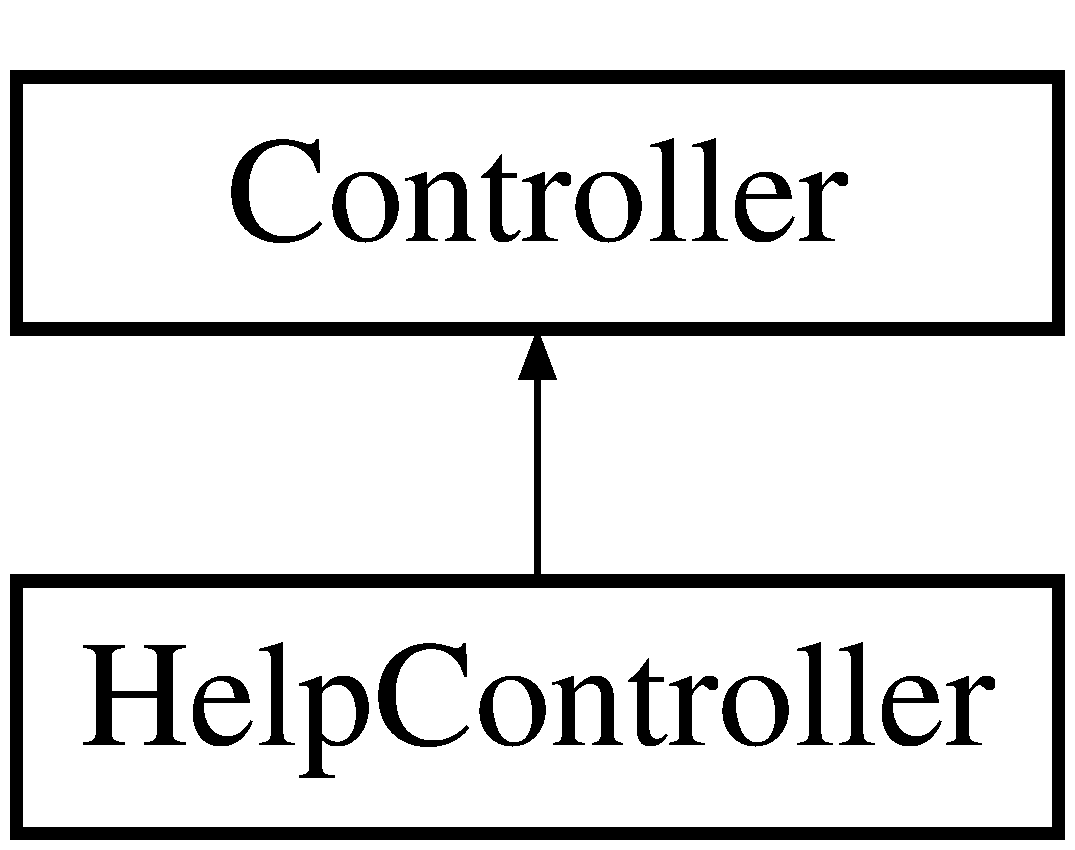
\includegraphics[height=2.000000cm]{classApi3Layers_1_1Areas_1_1HelpPage_1_1Controllers_1_1HelpController}
\end{center}
\end{figure}
\subsection*{Métodos Públicos}
\begin{DoxyCompactItemize}
\item 
\hyperlink{classApi3Layers_1_1Areas_1_1HelpPage_1_1Controllers_1_1HelpController_a83181268f5f82b22c63b3f978fa4c32c}{Help\+Controller} ()
\item 
\hyperlink{classApi3Layers_1_1Areas_1_1HelpPage_1_1Controllers_1_1HelpController_a7fb80807bac7887eefc2cf102ad34d7a}{Help\+Controller} (Http\+Configuration config)
\item 
Action\+Result \hyperlink{classApi3Layers_1_1Areas_1_1HelpPage_1_1Controllers_1_1HelpController_a7ab3cc2e28440430c53c8651bee60e72}{Api} (string api\+Id)
\item 
Action\+Result \hyperlink{classApi3Layers_1_1Areas_1_1HelpPage_1_1Controllers_1_1HelpController_a82bdd581a9c68d02c11ac8160aa5d60b}{Index} ()
\item 
Action\+Result \hyperlink{classApi3Layers_1_1Areas_1_1HelpPage_1_1Controllers_1_1HelpController_a6833392bcc6273de228714a6f512c2bc}{Resource\+Model} (string model\+Name)
\end{DoxyCompactItemize}
\subsection*{Propriedades}
\begin{DoxyCompactItemize}
\item 
Http\+Configuration \hyperlink{classApi3Layers_1_1Areas_1_1HelpPage_1_1Controllers_1_1HelpController_aa3cd9c8489aca78a2da59567fc5207ba}{Configuration}\hspace{0.3cm}{\ttfamily  \mbox{[}get, private set\mbox{]}}
\end{DoxyCompactItemize}
\subsection*{Atributos Privados}
\begin{DoxyCompactItemize}
\item 
const string \hyperlink{classApi3Layers_1_1Areas_1_1HelpPage_1_1Controllers_1_1HelpController_abb8799c1a3b97aa220ff62e1ab8a4175}{Error\+View\+Name} = \char`\"{}Error\char`\"{}
\end{DoxyCompactItemize}


\subsection{Descrição Detalhada}
The controller that will handle requests for the help page. 



\subsection{Construtores \& Destrutores}
\mbox{\Hypertarget{classApi3Layers_1_1Areas_1_1HelpPage_1_1Controllers_1_1HelpController_a83181268f5f82b22c63b3f978fa4c32c}\label{classApi3Layers_1_1Areas_1_1HelpPage_1_1Controllers_1_1HelpController_a83181268f5f82b22c63b3f978fa4c32c}} 
\index{Api3\+Layers\+::\+Areas\+::\+Help\+Page\+::\+Controllers\+::\+Help\+Controller@{Api3\+Layers\+::\+Areas\+::\+Help\+Page\+::\+Controllers\+::\+Help\+Controller}!Help\+Controller@{Help\+Controller}}
\index{Help\+Controller@{Help\+Controller}!Api3\+Layers\+::\+Areas\+::\+Help\+Page\+::\+Controllers\+::\+Help\+Controller@{Api3\+Layers\+::\+Areas\+::\+Help\+Page\+::\+Controllers\+::\+Help\+Controller}}
\subsubsection{\texorpdfstring{Help\+Controller()}{HelpController()}\hspace{0.1cm}{\footnotesize\ttfamily [1/2]}}
{\footnotesize\ttfamily \hyperlink{classApi3Layers_1_1Areas_1_1HelpPage_1_1Controllers_1_1HelpController}{Help\+Controller} (\begin{DoxyParamCaption}{ }\end{DoxyParamCaption})}

\mbox{\Hypertarget{classApi3Layers_1_1Areas_1_1HelpPage_1_1Controllers_1_1HelpController_a7fb80807bac7887eefc2cf102ad34d7a}\label{classApi3Layers_1_1Areas_1_1HelpPage_1_1Controllers_1_1HelpController_a7fb80807bac7887eefc2cf102ad34d7a}} 
\index{Api3\+Layers\+::\+Areas\+::\+Help\+Page\+::\+Controllers\+::\+Help\+Controller@{Api3\+Layers\+::\+Areas\+::\+Help\+Page\+::\+Controllers\+::\+Help\+Controller}!Help\+Controller@{Help\+Controller}}
\index{Help\+Controller@{Help\+Controller}!Api3\+Layers\+::\+Areas\+::\+Help\+Page\+::\+Controllers\+::\+Help\+Controller@{Api3\+Layers\+::\+Areas\+::\+Help\+Page\+::\+Controllers\+::\+Help\+Controller}}
\subsubsection{\texorpdfstring{Help\+Controller()}{HelpController()}\hspace{0.1cm}{\footnotesize\ttfamily [2/2]}}
{\footnotesize\ttfamily \hyperlink{classApi3Layers_1_1Areas_1_1HelpPage_1_1Controllers_1_1HelpController}{Help\+Controller} (\begin{DoxyParamCaption}\item[{Http\+Configuration}]{config }\end{DoxyParamCaption})}



\subsection{Métodos}
\mbox{\Hypertarget{classApi3Layers_1_1Areas_1_1HelpPage_1_1Controllers_1_1HelpController_a7ab3cc2e28440430c53c8651bee60e72}\label{classApi3Layers_1_1Areas_1_1HelpPage_1_1Controllers_1_1HelpController_a7ab3cc2e28440430c53c8651bee60e72}} 
\index{Api3\+Layers\+::\+Areas\+::\+Help\+Page\+::\+Controllers\+::\+Help\+Controller@{Api3\+Layers\+::\+Areas\+::\+Help\+Page\+::\+Controllers\+::\+Help\+Controller}!Api@{Api}}
\index{Api@{Api}!Api3\+Layers\+::\+Areas\+::\+Help\+Page\+::\+Controllers\+::\+Help\+Controller@{Api3\+Layers\+::\+Areas\+::\+Help\+Page\+::\+Controllers\+::\+Help\+Controller}}
\subsubsection{\texorpdfstring{Api()}{Api()}}
{\footnotesize\ttfamily Action\+Result Api (\begin{DoxyParamCaption}\item[{string}]{api\+Id }\end{DoxyParamCaption})}

\mbox{\Hypertarget{classApi3Layers_1_1Areas_1_1HelpPage_1_1Controllers_1_1HelpController_a82bdd581a9c68d02c11ac8160aa5d60b}\label{classApi3Layers_1_1Areas_1_1HelpPage_1_1Controllers_1_1HelpController_a82bdd581a9c68d02c11ac8160aa5d60b}} 
\index{Api3\+Layers\+::\+Areas\+::\+Help\+Page\+::\+Controllers\+::\+Help\+Controller@{Api3\+Layers\+::\+Areas\+::\+Help\+Page\+::\+Controllers\+::\+Help\+Controller}!Index@{Index}}
\index{Index@{Index}!Api3\+Layers\+::\+Areas\+::\+Help\+Page\+::\+Controllers\+::\+Help\+Controller@{Api3\+Layers\+::\+Areas\+::\+Help\+Page\+::\+Controllers\+::\+Help\+Controller}}
\subsubsection{\texorpdfstring{Index()}{Index()}}
{\footnotesize\ttfamily Action\+Result Index (\begin{DoxyParamCaption}{ }\end{DoxyParamCaption})}

\mbox{\Hypertarget{classApi3Layers_1_1Areas_1_1HelpPage_1_1Controllers_1_1HelpController_a6833392bcc6273de228714a6f512c2bc}\label{classApi3Layers_1_1Areas_1_1HelpPage_1_1Controllers_1_1HelpController_a6833392bcc6273de228714a6f512c2bc}} 
\index{Api3\+Layers\+::\+Areas\+::\+Help\+Page\+::\+Controllers\+::\+Help\+Controller@{Api3\+Layers\+::\+Areas\+::\+Help\+Page\+::\+Controllers\+::\+Help\+Controller}!Resource\+Model@{Resource\+Model}}
\index{Resource\+Model@{Resource\+Model}!Api3\+Layers\+::\+Areas\+::\+Help\+Page\+::\+Controllers\+::\+Help\+Controller@{Api3\+Layers\+::\+Areas\+::\+Help\+Page\+::\+Controllers\+::\+Help\+Controller}}
\subsubsection{\texorpdfstring{Resource\+Model()}{ResourceModel()}}
{\footnotesize\ttfamily Action\+Result Resource\+Model (\begin{DoxyParamCaption}\item[{string}]{model\+Name }\end{DoxyParamCaption})}



\subsection{Atributos}
\mbox{\Hypertarget{classApi3Layers_1_1Areas_1_1HelpPage_1_1Controllers_1_1HelpController_abb8799c1a3b97aa220ff62e1ab8a4175}\label{classApi3Layers_1_1Areas_1_1HelpPage_1_1Controllers_1_1HelpController_abb8799c1a3b97aa220ff62e1ab8a4175}} 
\index{Api3\+Layers\+::\+Areas\+::\+Help\+Page\+::\+Controllers\+::\+Help\+Controller@{Api3\+Layers\+::\+Areas\+::\+Help\+Page\+::\+Controllers\+::\+Help\+Controller}!Error\+View\+Name@{Error\+View\+Name}}
\index{Error\+View\+Name@{Error\+View\+Name}!Api3\+Layers\+::\+Areas\+::\+Help\+Page\+::\+Controllers\+::\+Help\+Controller@{Api3\+Layers\+::\+Areas\+::\+Help\+Page\+::\+Controllers\+::\+Help\+Controller}}
\subsubsection{\texorpdfstring{Error\+View\+Name}{ErrorViewName}}
{\footnotesize\ttfamily const string Error\+View\+Name = \char`\"{}Error\char`\"{}\hspace{0.3cm}{\ttfamily [private]}}



\subsection{Propriedades}
\mbox{\Hypertarget{classApi3Layers_1_1Areas_1_1HelpPage_1_1Controllers_1_1HelpController_aa3cd9c8489aca78a2da59567fc5207ba}\label{classApi3Layers_1_1Areas_1_1HelpPage_1_1Controllers_1_1HelpController_aa3cd9c8489aca78a2da59567fc5207ba}} 
\index{Api3\+Layers\+::\+Areas\+::\+Help\+Page\+::\+Controllers\+::\+Help\+Controller@{Api3\+Layers\+::\+Areas\+::\+Help\+Page\+::\+Controllers\+::\+Help\+Controller}!Configuration@{Configuration}}
\index{Configuration@{Configuration}!Api3\+Layers\+::\+Areas\+::\+Help\+Page\+::\+Controllers\+::\+Help\+Controller@{Api3\+Layers\+::\+Areas\+::\+Help\+Page\+::\+Controllers\+::\+Help\+Controller}}
\subsubsection{\texorpdfstring{Configuration}{Configuration}}
{\footnotesize\ttfamily Http\+Configuration Configuration\hspace{0.3cm}{\ttfamily [get]}, {\ttfamily [private set]}}



A documentação para esta classe foi gerada a partir do seguinte arquivo\+:\begin{DoxyCompactItemize}
\item 
Api3\+Layers/\+Areas/\+Help\+Page/\+Controllers/\hyperlink{HelpController_8cs}{Help\+Controller.\+cs}\end{DoxyCompactItemize}

\hypertarget{classApi3Layers_1_1Areas_1_1HelpPage_1_1HelpPageAreaRegistration}{}\section{Help\+Page\+Area\+Registration}
\label{classApi3Layers_1_1Areas_1_1HelpPage_1_1HelpPageAreaRegistration}\index{Help\+Page\+Area\+Registration@{Help\+Page\+Area\+Registration}}
Diagrama de Hierarquia para Help\+Page\+Area\+Registration\+:\begin{figure}[H]
\begin{center}
\leavevmode
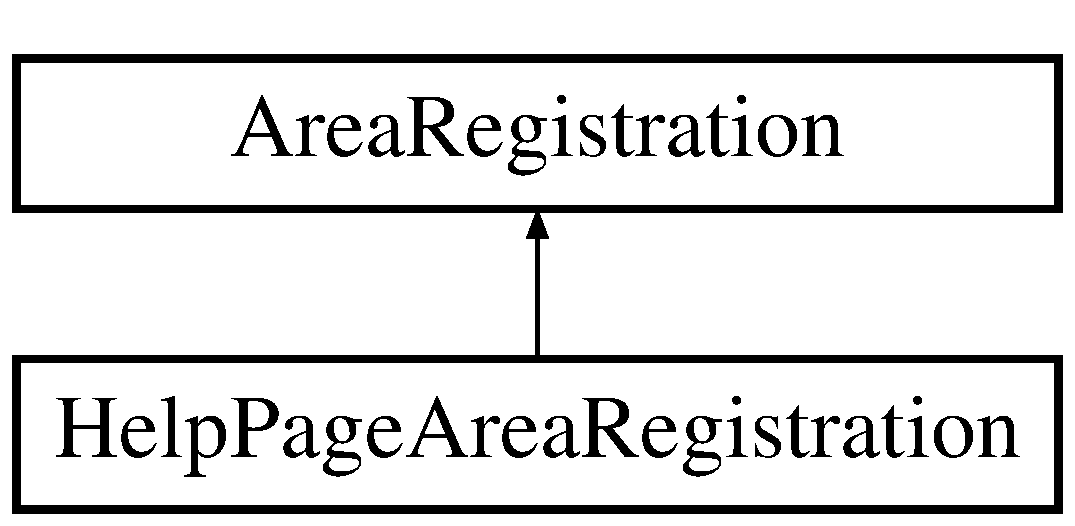
\includegraphics[height=2.000000cm]{dd/df1/classApi3Layers_1_1Areas_1_1HelpPage_1_1HelpPageAreaRegistration}
\end{center}
\end{figure}
\subsection*{Métodos Públicos}
\begin{DoxyCompactItemize}
\item 
override void \hyperlink{classApi3Layers_1_1Areas_1_1HelpPage_1_1HelpPageAreaRegistration_a7c67c594ee2be5522d6bb422ba337e94}{Register\+Area} (Area\+Registration\+Context context)
\end{DoxyCompactItemize}
\subsection*{Propriedades}
\begin{DoxyCompactItemize}
\item 
override string \hyperlink{classApi3Layers_1_1Areas_1_1HelpPage_1_1HelpPageAreaRegistration_acf6f429626f20687e61c64d5d5dd9f6d}{Area\+Name}\hspace{0.3cm}{\ttfamily  \mbox{[}get\mbox{]}}
\end{DoxyCompactItemize}


\subsection{Métodos}
\mbox{\Hypertarget{classApi3Layers_1_1Areas_1_1HelpPage_1_1HelpPageAreaRegistration_a7c67c594ee2be5522d6bb422ba337e94}\label{classApi3Layers_1_1Areas_1_1HelpPage_1_1HelpPageAreaRegistration_a7c67c594ee2be5522d6bb422ba337e94}} 
\index{Api3\+Layers\+::\+Areas\+::\+Help\+Page\+::\+Help\+Page\+Area\+Registration@{Api3\+Layers\+::\+Areas\+::\+Help\+Page\+::\+Help\+Page\+Area\+Registration}!Register\+Area@{Register\+Area}}
\index{Register\+Area@{Register\+Area}!Api3\+Layers\+::\+Areas\+::\+Help\+Page\+::\+Help\+Page\+Area\+Registration@{Api3\+Layers\+::\+Areas\+::\+Help\+Page\+::\+Help\+Page\+Area\+Registration}}
\subsubsection{\texorpdfstring{Register\+Area()}{RegisterArea()}}
{\footnotesize\ttfamily override void Register\+Area (\begin{DoxyParamCaption}\item[{Area\+Registration\+Context}]{context }\end{DoxyParamCaption})}



\subsection{Propriedades}
\mbox{\Hypertarget{classApi3Layers_1_1Areas_1_1HelpPage_1_1HelpPageAreaRegistration_acf6f429626f20687e61c64d5d5dd9f6d}\label{classApi3Layers_1_1Areas_1_1HelpPage_1_1HelpPageAreaRegistration_acf6f429626f20687e61c64d5d5dd9f6d}} 
\index{Api3\+Layers\+::\+Areas\+::\+Help\+Page\+::\+Help\+Page\+Area\+Registration@{Api3\+Layers\+::\+Areas\+::\+Help\+Page\+::\+Help\+Page\+Area\+Registration}!Area\+Name@{Area\+Name}}
\index{Area\+Name@{Area\+Name}!Api3\+Layers\+::\+Areas\+::\+Help\+Page\+::\+Help\+Page\+Area\+Registration@{Api3\+Layers\+::\+Areas\+::\+Help\+Page\+::\+Help\+Page\+Area\+Registration}}
\subsubsection{\texorpdfstring{Area\+Name}{AreaName}}
{\footnotesize\ttfamily override string Area\+Name\hspace{0.3cm}{\ttfamily [get]}}



A documentação para esta classe foi gerada a partir do seguinte arquivo\+:\begin{DoxyCompactItemize}
\item 
C\+:/\+Users/\+Bruno/\+Desktop/\+Api3\+Layers/\+Api3\+Layers/\+Areas/\+Help\+Page/\hyperlink{HelpPageAreaRegistration_8cs}{Help\+Page\+Area\+Registration.\+cs}\end{DoxyCompactItemize}

\hypertarget{classApi3Layers_1_1Areas_1_1HelpPage_1_1HelpPageConfig}{}\section{Help\+Page\+Config}
\label{classApi3Layers_1_1Areas_1_1HelpPage_1_1HelpPageConfig}\index{Help\+Page\+Config@{Help\+Page\+Config}}


Use this class to customize the Help Page. For example you can set a custom System.\+Web.\+Http.\+Description.\+I\+Documentation\+Provider to supply the documentation or you can provide the samples for the requests/responses.  


\subsection*{Métodos Públicos Estáticos}
\begin{DoxyCompactItemize}
\item 
static void \hyperlink{classApi3Layers_1_1Areas_1_1HelpPage_1_1HelpPageConfig_a8941f9a1c4d63842b463068258264cf4}{Register} (Http\+Configuration config)
\end{DoxyCompactItemize}


\subsection{Descrição Detalhada}
Use this class to customize the Help Page. For example you can set a custom System.\+Web.\+Http.\+Description.\+I\+Documentation\+Provider to supply the documentation or you can provide the samples for the requests/responses. 



\subsection{Métodos}
\mbox{\Hypertarget{classApi3Layers_1_1Areas_1_1HelpPage_1_1HelpPageConfig_a8941f9a1c4d63842b463068258264cf4}\label{classApi3Layers_1_1Areas_1_1HelpPage_1_1HelpPageConfig_a8941f9a1c4d63842b463068258264cf4}} 
\index{Api3\+Layers\+::\+Areas\+::\+Help\+Page\+::\+Help\+Page\+Config@{Api3\+Layers\+::\+Areas\+::\+Help\+Page\+::\+Help\+Page\+Config}!Register@{Register}}
\index{Register@{Register}!Api3\+Layers\+::\+Areas\+::\+Help\+Page\+::\+Help\+Page\+Config@{Api3\+Layers\+::\+Areas\+::\+Help\+Page\+::\+Help\+Page\+Config}}
\subsubsection{\texorpdfstring{Register()}{Register()}}
{\footnotesize\ttfamily static void Register (\begin{DoxyParamCaption}\item[{Http\+Configuration}]{config }\end{DoxyParamCaption})\hspace{0.3cm}{\ttfamily [static]}}



A documentação para esta classe foi gerada a partir do seguinte arquivo\+:\begin{DoxyCompactItemize}
\item 
C\+:/\+Users/\+Bruno/\+Desktop/\+Api3\+Layers/\+Api3\+Layers/\+Areas/\+Help\+Page/\+App\+\_\+\+Start/\hyperlink{HelpPageConfig_8cs}{Help\+Page\+Config.\+cs}\end{DoxyCompactItemize}

\hypertarget{classApi3Layers_1_1Areas_1_1HelpPage_1_1HelpPageConfigurationExtensions}{}\section{Help\+Page\+Configuration\+Extensions}
\label{classApi3Layers_1_1Areas_1_1HelpPage_1_1HelpPageConfigurationExtensions}\index{Help\+Page\+Configuration\+Extensions@{Help\+Page\+Configuration\+Extensions}}
\subsection*{Métodos Públicos Estáticos}
\begin{DoxyCompactItemize}
\item 
static \hyperlink{classApi3Layers_1_1Areas_1_1HelpPage_1_1Models_1_1HelpPageApiModel}{Help\+Page\+Api\+Model} \hyperlink{classApi3Layers_1_1Areas_1_1HelpPage_1_1HelpPageConfigurationExtensions_a8e1dd06343ebfd465042fb7fde291909}{Get\+Help\+Page\+Api\+Model} (this Http\+Configuration config, string api\+Description\+Id)
\begin{DoxyCompactList}\small\item\em Gets the model that represents an A\+PI displayed on the help page. The model is initialized on the first call and cached for subsequent calls. \end{DoxyCompactList}\item 
static \hyperlink{classApi3Layers_1_1Areas_1_1HelpPage_1_1HelpPageSampleGenerator}{Help\+Page\+Sample\+Generator} \hyperlink{classApi3Layers_1_1Areas_1_1HelpPage_1_1HelpPageConfigurationExtensions_a7f67d57eac84d585f41aabeb28ae7bd0}{Get\+Help\+Page\+Sample\+Generator} (this Http\+Configuration config)
\begin{DoxyCompactList}\small\item\em Gets the help page sample generator. \end{DoxyCompactList}\item 
static \hyperlink{classApi3Layers_1_1Areas_1_1HelpPage_1_1ModelDescriptions_1_1ModelDescriptionGenerator}{Model\+Description\+Generator} \hyperlink{classApi3Layers_1_1Areas_1_1HelpPage_1_1HelpPageConfigurationExtensions_aa3345ea75f3272cdc05598cceeddd7a9}{Get\+Model\+Description\+Generator} (this Http\+Configuration config)
\begin{DoxyCompactList}\small\item\em Gets the model description generator. \end{DoxyCompactList}\item 
static void \hyperlink{classApi3Layers_1_1Areas_1_1HelpPage_1_1HelpPageConfigurationExtensions_a977618c0c67efa9733ed109a3f730409}{Set\+Actual\+Request\+Type} (this Http\+Configuration config, Type type, string controller\+Name, string action\+Name)
\begin{DoxyCompactList}\small\item\em Specifies the actual type of System.\+Net.\+Http.\+Object\+Content$<$\+T$>$ passed to the System.\+Net.\+Http.\+Http\+Request\+Message in an action. The help page will use this information to produce more accurate request samples. \end{DoxyCompactList}\item 
static void \hyperlink{classApi3Layers_1_1Areas_1_1HelpPage_1_1HelpPageConfigurationExtensions_ab354c6439434e49c51e02a5a1d37f160}{Set\+Actual\+Request\+Type} (this Http\+Configuration config, Type type, string controller\+Name, string action\+Name, params string\mbox{[}$\,$\mbox{]} parameter\+Names)
\begin{DoxyCompactList}\small\item\em Specifies the actual type of System.\+Net.\+Http.\+Object\+Content$<$\+T$>$ passed to the System.\+Net.\+Http.\+Http\+Request\+Message in an action. The help page will use this information to produce more accurate request samples. \end{DoxyCompactList}\item 
static void \hyperlink{classApi3Layers_1_1Areas_1_1HelpPage_1_1HelpPageConfigurationExtensions_a7cb7f27af68b6ee4e745f021ec1b556a}{Set\+Actual\+Response\+Type} (this Http\+Configuration config, Type type, string controller\+Name, string action\+Name)
\begin{DoxyCompactList}\small\item\em Specifies the actual type of System.\+Net.\+Http.\+Object\+Content$<$\+T$>$ returned as part of the System.\+Net.\+Http.\+Http\+Request\+Message in an action. The help page will use this information to produce more accurate response samples. \end{DoxyCompactList}\item 
static void \hyperlink{classApi3Layers_1_1Areas_1_1HelpPage_1_1HelpPageConfigurationExtensions_adba814aa7b0c89363674b03b2f7e93ef}{Set\+Actual\+Response\+Type} (this Http\+Configuration config, Type type, string controller\+Name, string action\+Name, params string\mbox{[}$\,$\mbox{]} parameter\+Names)
\begin{DoxyCompactList}\small\item\em Specifies the actual type of System.\+Net.\+Http.\+Object\+Content$<$\+T$>$ returned as part of the System.\+Net.\+Http.\+Http\+Request\+Message in an action. The help page will use this information to produce more accurate response samples. \end{DoxyCompactList}\item 
static void \hyperlink{classApi3Layers_1_1Areas_1_1HelpPage_1_1HelpPageConfigurationExtensions_af10aae8f181e9989cbf3183a7dd297c7}{Set\+Documentation\+Provider} (this Http\+Configuration config, I\+Documentation\+Provider documentation\+Provider)
\begin{DoxyCompactList}\small\item\em Sets the documentation provider for help page. \end{DoxyCompactList}\item 
static void \hyperlink{classApi3Layers_1_1Areas_1_1HelpPage_1_1HelpPageConfigurationExtensions_a4788b1a5481baebf9302bad07fa4d784}{Set\+Help\+Page\+Sample\+Generator} (this Http\+Configuration config, \hyperlink{classApi3Layers_1_1Areas_1_1HelpPage_1_1HelpPageSampleGenerator}{Help\+Page\+Sample\+Generator} sample\+Generator)
\begin{DoxyCompactList}\small\item\em Sets the help page sample generator. \end{DoxyCompactList}\item 
static void \hyperlink{classApi3Layers_1_1Areas_1_1HelpPage_1_1HelpPageConfigurationExtensions_af6ec1b6adfbeb0c61221bb7eeed98c8e}{Set\+Sample\+For\+Media\+Type} (this Http\+Configuration config, object sample, Media\+Type\+Header\+Value media\+Type)
\begin{DoxyCompactList}\small\item\em Sets the sample directly for all actions with the specified media type. \end{DoxyCompactList}\item 
static void \hyperlink{classApi3Layers_1_1Areas_1_1HelpPage_1_1HelpPageConfigurationExtensions_ac4e9d3ce5bc78349ee756b5eae07718a}{Set\+Sample\+For\+Type} (this Http\+Configuration config, object sample, Media\+Type\+Header\+Value media\+Type, Type type)
\begin{DoxyCompactList}\small\item\em Sets the sample directly for all actions with the specified type and media type. \end{DoxyCompactList}\item 
static void \hyperlink{classApi3Layers_1_1Areas_1_1HelpPage_1_1HelpPageConfigurationExtensions_a0578ea8446c286c76da516e819fe253c}{Set\+Sample\+Objects} (this Http\+Configuration config, I\+Dictionary$<$ Type, object $>$ sample\+Objects)
\begin{DoxyCompactList}\small\item\em Sets the objects that will be used by the formatters to produce sample requests/responses. \end{DoxyCompactList}\item 
static void \hyperlink{classApi3Layers_1_1Areas_1_1HelpPage_1_1HelpPageConfigurationExtensions_a82bd1788448158adaca5a19be618f630}{Set\+Sample\+Request} (this Http\+Configuration config, object sample, Media\+Type\+Header\+Value media\+Type, string controller\+Name, string action\+Name)
\begin{DoxyCompactList}\small\item\em Sets the sample request directly for the specified media type and action. \end{DoxyCompactList}\item 
static void \hyperlink{classApi3Layers_1_1Areas_1_1HelpPage_1_1HelpPageConfigurationExtensions_a1974e4f7b6984e2dbd16badf7700a505}{Set\+Sample\+Request} (this Http\+Configuration config, object sample, Media\+Type\+Header\+Value media\+Type, string controller\+Name, string action\+Name, params string\mbox{[}$\,$\mbox{]} parameter\+Names)
\begin{DoxyCompactList}\small\item\em Sets the sample request directly for the specified media type and action with parameters. \end{DoxyCompactList}\item 
static void \hyperlink{classApi3Layers_1_1Areas_1_1HelpPage_1_1HelpPageConfigurationExtensions_a51e9644a90326e7a1927c78a8d1e346b}{Set\+Sample\+Response} (this Http\+Configuration config, object sample, Media\+Type\+Header\+Value media\+Type, string controller\+Name, string action\+Name)
\begin{DoxyCompactList}\small\item\em Sets the sample request directly for the specified media type of the action. \end{DoxyCompactList}\item 
static void \hyperlink{classApi3Layers_1_1Areas_1_1HelpPage_1_1HelpPageConfigurationExtensions_a5a807eb4c15e3e12fc45ccaca4c87603}{Set\+Sample\+Response} (this Http\+Configuration config, object sample, Media\+Type\+Header\+Value media\+Type, string controller\+Name, string action\+Name, params string\mbox{[}$\,$\mbox{]} parameter\+Names)
\begin{DoxyCompactList}\small\item\em Sets the sample response directly for the specified media type of the action with specific parameters. \end{DoxyCompactList}\end{DoxyCompactItemize}
\subsection*{Métodos Privados Estáticos}
\begin{DoxyCompactItemize}
\item 
static \hyperlink{classApi3Layers_1_1Areas_1_1HelpPage_1_1ModelDescriptions_1_1ParameterDescription}{Parameter\+Description} \hyperlink{classApi3Layers_1_1Areas_1_1HelpPage_1_1HelpPageConfigurationExtensions_ab6eed27114a1a255723fa4ab8a65586d}{Add\+Parameter\+Description} (\hyperlink{classApi3Layers_1_1Areas_1_1HelpPage_1_1Models_1_1HelpPageApiModel}{Help\+Page\+Api\+Model} api\+Model, Api\+Parameter\+Description api\+Parameter, \hyperlink{classApi3Layers_1_1Areas_1_1HelpPage_1_1ModelDescriptions_1_1ModelDescription}{Model\+Description} type\+Description)
\item 
static \hyperlink{classApi3Layers_1_1Areas_1_1HelpPage_1_1Models_1_1HelpPageApiModel}{Help\+Page\+Api\+Model} \hyperlink{classApi3Layers_1_1Areas_1_1HelpPage_1_1HelpPageConfigurationExtensions_a3008459bcff41d3002541c3ff407e712}{Generate\+Api\+Model} (Api\+Description api\+Description, Http\+Configuration config)
\item 
static void \hyperlink{classApi3Layers_1_1Areas_1_1HelpPage_1_1HelpPageConfigurationExtensions_af01d383426748f527ebe3c07e9f8a4bc}{Generate\+Request\+Model\+Description} (\hyperlink{classApi3Layers_1_1Areas_1_1HelpPage_1_1Models_1_1HelpPageApiModel}{Help\+Page\+Api\+Model} api\+Model, \hyperlink{classApi3Layers_1_1Areas_1_1HelpPage_1_1ModelDescriptions_1_1ModelDescriptionGenerator}{Model\+Description\+Generator} model\+Generator, \hyperlink{classApi3Layers_1_1Areas_1_1HelpPage_1_1HelpPageSampleGenerator}{Help\+Page\+Sample\+Generator} sample\+Generator)
\item 
static void \hyperlink{classApi3Layers_1_1Areas_1_1HelpPage_1_1HelpPageConfigurationExtensions_ad4296fc92e40d842eb654298d2ed3e7e}{Generate\+Resource\+Description} (\hyperlink{classApi3Layers_1_1Areas_1_1HelpPage_1_1Models_1_1HelpPageApiModel}{Help\+Page\+Api\+Model} api\+Model, \hyperlink{classApi3Layers_1_1Areas_1_1HelpPage_1_1ModelDescriptions_1_1ModelDescriptionGenerator}{Model\+Description\+Generator} model\+Generator)
\item 
static void \hyperlink{classApi3Layers_1_1Areas_1_1HelpPage_1_1HelpPageConfigurationExtensions_ad2943e71c3adf193fbfdc68e06d35898}{Generate\+Samples} (\hyperlink{classApi3Layers_1_1Areas_1_1HelpPage_1_1Models_1_1HelpPageApiModel}{Help\+Page\+Api\+Model} api\+Model, \hyperlink{classApi3Layers_1_1Areas_1_1HelpPage_1_1HelpPageSampleGenerator}{Help\+Page\+Sample\+Generator} sample\+Generator)
\item 
static void \hyperlink{classApi3Layers_1_1Areas_1_1HelpPage_1_1HelpPageConfigurationExtensions_af3b2401673b568e9a8db7b2627fc031d}{Generate\+Uri\+Parameters} (\hyperlink{classApi3Layers_1_1Areas_1_1HelpPage_1_1Models_1_1HelpPageApiModel}{Help\+Page\+Api\+Model} api\+Model, \hyperlink{classApi3Layers_1_1Areas_1_1HelpPage_1_1ModelDescriptions_1_1ModelDescriptionGenerator}{Model\+Description\+Generator} model\+Generator)
\item 
static \hyperlink{classApi3Layers_1_1Areas_1_1HelpPage_1_1ModelDescriptions_1_1ModelDescriptionGenerator}{Model\+Description\+Generator} \hyperlink{classApi3Layers_1_1Areas_1_1HelpPage_1_1HelpPageConfigurationExtensions_a16f47e8aa323c09cd0cf32e89db952bf}{Initialize\+Model\+Description\+Generator} (Http\+Configuration config)
\item 
static bool \hyperlink{classApi3Layers_1_1Areas_1_1HelpPage_1_1HelpPageConfigurationExtensions_a732c7e4cbb02fe025f256f3d4474b914}{Is\+Bindable\+With\+Type\+Converter} (Type parameter\+Type)
\item 
static void \hyperlink{classApi3Layers_1_1Areas_1_1HelpPage_1_1HelpPageConfigurationExtensions_ab46e5f234a0f063dfaf277f77ddee2f6}{Log\+Invalid\+Sample\+As\+Error} (\hyperlink{classApi3Layers_1_1Areas_1_1HelpPage_1_1Models_1_1HelpPageApiModel}{Help\+Page\+Api\+Model} api\+Model, object sample)
\item 
static bool \hyperlink{classApi3Layers_1_1Areas_1_1HelpPage_1_1HelpPageConfigurationExtensions_ad4d11c54254ca636a77a9cc8aef8c46e}{Try\+Get\+Resource\+Parameter} (Api\+Description api\+Description, Http\+Configuration config, out Api\+Parameter\+Description parameter\+Description, out Type resource\+Type)
\end{DoxyCompactItemize}
\subsection*{Atributos Privados}
\begin{DoxyCompactItemize}
\item 
const string \hyperlink{classApi3Layers_1_1Areas_1_1HelpPage_1_1HelpPageConfigurationExtensions_a04d4e06a2bc79e7cf9f3acb633928c3a}{Api\+Model\+Prefix} = \char`\"{}M\+S\+\_\+\+Help\+Page\+Api\+Model\+\_\+\char`\"{}
\end{DoxyCompactItemize}


\subsection{Métodos}
\mbox{\Hypertarget{classApi3Layers_1_1Areas_1_1HelpPage_1_1HelpPageConfigurationExtensions_ab6eed27114a1a255723fa4ab8a65586d}\label{classApi3Layers_1_1Areas_1_1HelpPage_1_1HelpPageConfigurationExtensions_ab6eed27114a1a255723fa4ab8a65586d}} 
\index{Api3\+Layers\+::\+Areas\+::\+Help\+Page\+::\+Help\+Page\+Configuration\+Extensions@{Api3\+Layers\+::\+Areas\+::\+Help\+Page\+::\+Help\+Page\+Configuration\+Extensions}!Add\+Parameter\+Description@{Add\+Parameter\+Description}}
\index{Add\+Parameter\+Description@{Add\+Parameter\+Description}!Api3\+Layers\+::\+Areas\+::\+Help\+Page\+::\+Help\+Page\+Configuration\+Extensions@{Api3\+Layers\+::\+Areas\+::\+Help\+Page\+::\+Help\+Page\+Configuration\+Extensions}}
\subsubsection{\texorpdfstring{Add\+Parameter\+Description()}{AddParameterDescription()}}
{\footnotesize\ttfamily static \hyperlink{classApi3Layers_1_1Areas_1_1HelpPage_1_1ModelDescriptions_1_1ParameterDescription}{Parameter\+Description} Add\+Parameter\+Description (\begin{DoxyParamCaption}\item[{\hyperlink{classApi3Layers_1_1Areas_1_1HelpPage_1_1Models_1_1HelpPageApiModel}{Help\+Page\+Api\+Model}}]{api\+Model,  }\item[{Api\+Parameter\+Description}]{api\+Parameter,  }\item[{\hyperlink{classApi3Layers_1_1Areas_1_1HelpPage_1_1ModelDescriptions_1_1ModelDescription}{Model\+Description}}]{type\+Description }\end{DoxyParamCaption})\hspace{0.3cm}{\ttfamily [static]}, {\ttfamily [private]}}

\mbox{\Hypertarget{classApi3Layers_1_1Areas_1_1HelpPage_1_1HelpPageConfigurationExtensions_a3008459bcff41d3002541c3ff407e712}\label{classApi3Layers_1_1Areas_1_1HelpPage_1_1HelpPageConfigurationExtensions_a3008459bcff41d3002541c3ff407e712}} 
\index{Api3\+Layers\+::\+Areas\+::\+Help\+Page\+::\+Help\+Page\+Configuration\+Extensions@{Api3\+Layers\+::\+Areas\+::\+Help\+Page\+::\+Help\+Page\+Configuration\+Extensions}!Generate\+Api\+Model@{Generate\+Api\+Model}}
\index{Generate\+Api\+Model@{Generate\+Api\+Model}!Api3\+Layers\+::\+Areas\+::\+Help\+Page\+::\+Help\+Page\+Configuration\+Extensions@{Api3\+Layers\+::\+Areas\+::\+Help\+Page\+::\+Help\+Page\+Configuration\+Extensions}}
\subsubsection{\texorpdfstring{Generate\+Api\+Model()}{GenerateApiModel()}}
{\footnotesize\ttfamily static \hyperlink{classApi3Layers_1_1Areas_1_1HelpPage_1_1Models_1_1HelpPageApiModel}{Help\+Page\+Api\+Model} Generate\+Api\+Model (\begin{DoxyParamCaption}\item[{Api\+Description}]{api\+Description,  }\item[{Http\+Configuration}]{config }\end{DoxyParamCaption})\hspace{0.3cm}{\ttfamily [static]}, {\ttfamily [private]}}

\mbox{\Hypertarget{classApi3Layers_1_1Areas_1_1HelpPage_1_1HelpPageConfigurationExtensions_af01d383426748f527ebe3c07e9f8a4bc}\label{classApi3Layers_1_1Areas_1_1HelpPage_1_1HelpPageConfigurationExtensions_af01d383426748f527ebe3c07e9f8a4bc}} 
\index{Api3\+Layers\+::\+Areas\+::\+Help\+Page\+::\+Help\+Page\+Configuration\+Extensions@{Api3\+Layers\+::\+Areas\+::\+Help\+Page\+::\+Help\+Page\+Configuration\+Extensions}!Generate\+Request\+Model\+Description@{Generate\+Request\+Model\+Description}}
\index{Generate\+Request\+Model\+Description@{Generate\+Request\+Model\+Description}!Api3\+Layers\+::\+Areas\+::\+Help\+Page\+::\+Help\+Page\+Configuration\+Extensions@{Api3\+Layers\+::\+Areas\+::\+Help\+Page\+::\+Help\+Page\+Configuration\+Extensions}}
\subsubsection{\texorpdfstring{Generate\+Request\+Model\+Description()}{GenerateRequestModelDescription()}}
{\footnotesize\ttfamily static void Generate\+Request\+Model\+Description (\begin{DoxyParamCaption}\item[{\hyperlink{classApi3Layers_1_1Areas_1_1HelpPage_1_1Models_1_1HelpPageApiModel}{Help\+Page\+Api\+Model}}]{api\+Model,  }\item[{\hyperlink{classApi3Layers_1_1Areas_1_1HelpPage_1_1ModelDescriptions_1_1ModelDescriptionGenerator}{Model\+Description\+Generator}}]{model\+Generator,  }\item[{\hyperlink{classApi3Layers_1_1Areas_1_1HelpPage_1_1HelpPageSampleGenerator}{Help\+Page\+Sample\+Generator}}]{sample\+Generator }\end{DoxyParamCaption})\hspace{0.3cm}{\ttfamily [static]}, {\ttfamily [private]}}

\mbox{\Hypertarget{classApi3Layers_1_1Areas_1_1HelpPage_1_1HelpPageConfigurationExtensions_ad4296fc92e40d842eb654298d2ed3e7e}\label{classApi3Layers_1_1Areas_1_1HelpPage_1_1HelpPageConfigurationExtensions_ad4296fc92e40d842eb654298d2ed3e7e}} 
\index{Api3\+Layers\+::\+Areas\+::\+Help\+Page\+::\+Help\+Page\+Configuration\+Extensions@{Api3\+Layers\+::\+Areas\+::\+Help\+Page\+::\+Help\+Page\+Configuration\+Extensions}!Generate\+Resource\+Description@{Generate\+Resource\+Description}}
\index{Generate\+Resource\+Description@{Generate\+Resource\+Description}!Api3\+Layers\+::\+Areas\+::\+Help\+Page\+::\+Help\+Page\+Configuration\+Extensions@{Api3\+Layers\+::\+Areas\+::\+Help\+Page\+::\+Help\+Page\+Configuration\+Extensions}}
\subsubsection{\texorpdfstring{Generate\+Resource\+Description()}{GenerateResourceDescription()}}
{\footnotesize\ttfamily static void Generate\+Resource\+Description (\begin{DoxyParamCaption}\item[{\hyperlink{classApi3Layers_1_1Areas_1_1HelpPage_1_1Models_1_1HelpPageApiModel}{Help\+Page\+Api\+Model}}]{api\+Model,  }\item[{\hyperlink{classApi3Layers_1_1Areas_1_1HelpPage_1_1ModelDescriptions_1_1ModelDescriptionGenerator}{Model\+Description\+Generator}}]{model\+Generator }\end{DoxyParamCaption})\hspace{0.3cm}{\ttfamily [static]}, {\ttfamily [private]}}

\mbox{\Hypertarget{classApi3Layers_1_1Areas_1_1HelpPage_1_1HelpPageConfigurationExtensions_ad2943e71c3adf193fbfdc68e06d35898}\label{classApi3Layers_1_1Areas_1_1HelpPage_1_1HelpPageConfigurationExtensions_ad2943e71c3adf193fbfdc68e06d35898}} 
\index{Api3\+Layers\+::\+Areas\+::\+Help\+Page\+::\+Help\+Page\+Configuration\+Extensions@{Api3\+Layers\+::\+Areas\+::\+Help\+Page\+::\+Help\+Page\+Configuration\+Extensions}!Generate\+Samples@{Generate\+Samples}}
\index{Generate\+Samples@{Generate\+Samples}!Api3\+Layers\+::\+Areas\+::\+Help\+Page\+::\+Help\+Page\+Configuration\+Extensions@{Api3\+Layers\+::\+Areas\+::\+Help\+Page\+::\+Help\+Page\+Configuration\+Extensions}}
\subsubsection{\texorpdfstring{Generate\+Samples()}{GenerateSamples()}}
{\footnotesize\ttfamily static void Generate\+Samples (\begin{DoxyParamCaption}\item[{\hyperlink{classApi3Layers_1_1Areas_1_1HelpPage_1_1Models_1_1HelpPageApiModel}{Help\+Page\+Api\+Model}}]{api\+Model,  }\item[{\hyperlink{classApi3Layers_1_1Areas_1_1HelpPage_1_1HelpPageSampleGenerator}{Help\+Page\+Sample\+Generator}}]{sample\+Generator }\end{DoxyParamCaption})\hspace{0.3cm}{\ttfamily [static]}, {\ttfamily [private]}}

\mbox{\Hypertarget{classApi3Layers_1_1Areas_1_1HelpPage_1_1HelpPageConfigurationExtensions_af3b2401673b568e9a8db7b2627fc031d}\label{classApi3Layers_1_1Areas_1_1HelpPage_1_1HelpPageConfigurationExtensions_af3b2401673b568e9a8db7b2627fc031d}} 
\index{Api3\+Layers\+::\+Areas\+::\+Help\+Page\+::\+Help\+Page\+Configuration\+Extensions@{Api3\+Layers\+::\+Areas\+::\+Help\+Page\+::\+Help\+Page\+Configuration\+Extensions}!Generate\+Uri\+Parameters@{Generate\+Uri\+Parameters}}
\index{Generate\+Uri\+Parameters@{Generate\+Uri\+Parameters}!Api3\+Layers\+::\+Areas\+::\+Help\+Page\+::\+Help\+Page\+Configuration\+Extensions@{Api3\+Layers\+::\+Areas\+::\+Help\+Page\+::\+Help\+Page\+Configuration\+Extensions}}
\subsubsection{\texorpdfstring{Generate\+Uri\+Parameters()}{GenerateUriParameters()}}
{\footnotesize\ttfamily static void Generate\+Uri\+Parameters (\begin{DoxyParamCaption}\item[{\hyperlink{classApi3Layers_1_1Areas_1_1HelpPage_1_1Models_1_1HelpPageApiModel}{Help\+Page\+Api\+Model}}]{api\+Model,  }\item[{\hyperlink{classApi3Layers_1_1Areas_1_1HelpPage_1_1ModelDescriptions_1_1ModelDescriptionGenerator}{Model\+Description\+Generator}}]{model\+Generator }\end{DoxyParamCaption})\hspace{0.3cm}{\ttfamily [static]}, {\ttfamily [private]}}

\mbox{\Hypertarget{classApi3Layers_1_1Areas_1_1HelpPage_1_1HelpPageConfigurationExtensions_a8e1dd06343ebfd465042fb7fde291909}\label{classApi3Layers_1_1Areas_1_1HelpPage_1_1HelpPageConfigurationExtensions_a8e1dd06343ebfd465042fb7fde291909}} 
\index{Api3\+Layers\+::\+Areas\+::\+Help\+Page\+::\+Help\+Page\+Configuration\+Extensions@{Api3\+Layers\+::\+Areas\+::\+Help\+Page\+::\+Help\+Page\+Configuration\+Extensions}!Get\+Help\+Page\+Api\+Model@{Get\+Help\+Page\+Api\+Model}}
\index{Get\+Help\+Page\+Api\+Model@{Get\+Help\+Page\+Api\+Model}!Api3\+Layers\+::\+Areas\+::\+Help\+Page\+::\+Help\+Page\+Configuration\+Extensions@{Api3\+Layers\+::\+Areas\+::\+Help\+Page\+::\+Help\+Page\+Configuration\+Extensions}}
\subsubsection{\texorpdfstring{Get\+Help\+Page\+Api\+Model()}{GetHelpPageApiModel()}}
{\footnotesize\ttfamily static \hyperlink{classApi3Layers_1_1Areas_1_1HelpPage_1_1Models_1_1HelpPageApiModel}{Help\+Page\+Api\+Model} Get\+Help\+Page\+Api\+Model (\begin{DoxyParamCaption}\item[{this Http\+Configuration}]{config,  }\item[{string}]{api\+Description\+Id }\end{DoxyParamCaption})\hspace{0.3cm}{\ttfamily [static]}}



Gets the model that represents an A\+PI displayed on the help page. The model is initialized on the first call and cached for subsequent calls. 


\begin{DoxyParams}{Parâmetros}
{\em config} & The Http\+Configuration.\\
\hline
{\em api\+Description\+Id} & The Api\+Description ID.\\
\hline
\end{DoxyParams}
\begin{DoxyReturn}{Retorna}
An Help\+Page\+Api\+Model 
\end{DoxyReturn}
\mbox{\Hypertarget{classApi3Layers_1_1Areas_1_1HelpPage_1_1HelpPageConfigurationExtensions_a7f67d57eac84d585f41aabeb28ae7bd0}\label{classApi3Layers_1_1Areas_1_1HelpPage_1_1HelpPageConfigurationExtensions_a7f67d57eac84d585f41aabeb28ae7bd0}} 
\index{Api3\+Layers\+::\+Areas\+::\+Help\+Page\+::\+Help\+Page\+Configuration\+Extensions@{Api3\+Layers\+::\+Areas\+::\+Help\+Page\+::\+Help\+Page\+Configuration\+Extensions}!Get\+Help\+Page\+Sample\+Generator@{Get\+Help\+Page\+Sample\+Generator}}
\index{Get\+Help\+Page\+Sample\+Generator@{Get\+Help\+Page\+Sample\+Generator}!Api3\+Layers\+::\+Areas\+::\+Help\+Page\+::\+Help\+Page\+Configuration\+Extensions@{Api3\+Layers\+::\+Areas\+::\+Help\+Page\+::\+Help\+Page\+Configuration\+Extensions}}
\subsubsection{\texorpdfstring{Get\+Help\+Page\+Sample\+Generator()}{GetHelpPageSampleGenerator()}}
{\footnotesize\ttfamily static \hyperlink{classApi3Layers_1_1Areas_1_1HelpPage_1_1HelpPageSampleGenerator}{Help\+Page\+Sample\+Generator} Get\+Help\+Page\+Sample\+Generator (\begin{DoxyParamCaption}\item[{this Http\+Configuration}]{config }\end{DoxyParamCaption})\hspace{0.3cm}{\ttfamily [static]}}



Gets the help page sample generator. 


\begin{DoxyParams}{Parâmetros}
{\em config} & The Http\+Configuration.\\
\hline
\end{DoxyParams}
\begin{DoxyReturn}{Retorna}
The help page sample generator.
\end{DoxyReturn}
\mbox{\Hypertarget{classApi3Layers_1_1Areas_1_1HelpPage_1_1HelpPageConfigurationExtensions_aa3345ea75f3272cdc05598cceeddd7a9}\label{classApi3Layers_1_1Areas_1_1HelpPage_1_1HelpPageConfigurationExtensions_aa3345ea75f3272cdc05598cceeddd7a9}} 
\index{Api3\+Layers\+::\+Areas\+::\+Help\+Page\+::\+Help\+Page\+Configuration\+Extensions@{Api3\+Layers\+::\+Areas\+::\+Help\+Page\+::\+Help\+Page\+Configuration\+Extensions}!Get\+Model\+Description\+Generator@{Get\+Model\+Description\+Generator}}
\index{Get\+Model\+Description\+Generator@{Get\+Model\+Description\+Generator}!Api3\+Layers\+::\+Areas\+::\+Help\+Page\+::\+Help\+Page\+Configuration\+Extensions@{Api3\+Layers\+::\+Areas\+::\+Help\+Page\+::\+Help\+Page\+Configuration\+Extensions}}
\subsubsection{\texorpdfstring{Get\+Model\+Description\+Generator()}{GetModelDescriptionGenerator()}}
{\footnotesize\ttfamily static \hyperlink{classApi3Layers_1_1Areas_1_1HelpPage_1_1ModelDescriptions_1_1ModelDescriptionGenerator}{Model\+Description\+Generator} Get\+Model\+Description\+Generator (\begin{DoxyParamCaption}\item[{this Http\+Configuration}]{config }\end{DoxyParamCaption})\hspace{0.3cm}{\ttfamily [static]}}



Gets the model description generator. 


\begin{DoxyParams}{Parâmetros}
{\em config} & The configuration.\\
\hline
\end{DoxyParams}
\begin{DoxyReturn}{Retorna}
The Model\+Description\+Generator
\end{DoxyReturn}
\mbox{\Hypertarget{classApi3Layers_1_1Areas_1_1HelpPage_1_1HelpPageConfigurationExtensions_a16f47e8aa323c09cd0cf32e89db952bf}\label{classApi3Layers_1_1Areas_1_1HelpPage_1_1HelpPageConfigurationExtensions_a16f47e8aa323c09cd0cf32e89db952bf}} 
\index{Api3\+Layers\+::\+Areas\+::\+Help\+Page\+::\+Help\+Page\+Configuration\+Extensions@{Api3\+Layers\+::\+Areas\+::\+Help\+Page\+::\+Help\+Page\+Configuration\+Extensions}!Initialize\+Model\+Description\+Generator@{Initialize\+Model\+Description\+Generator}}
\index{Initialize\+Model\+Description\+Generator@{Initialize\+Model\+Description\+Generator}!Api3\+Layers\+::\+Areas\+::\+Help\+Page\+::\+Help\+Page\+Configuration\+Extensions@{Api3\+Layers\+::\+Areas\+::\+Help\+Page\+::\+Help\+Page\+Configuration\+Extensions}}
\subsubsection{\texorpdfstring{Initialize\+Model\+Description\+Generator()}{InitializeModelDescriptionGenerator()}}
{\footnotesize\ttfamily static \hyperlink{classApi3Layers_1_1Areas_1_1HelpPage_1_1ModelDescriptions_1_1ModelDescriptionGenerator}{Model\+Description\+Generator} Initialize\+Model\+Description\+Generator (\begin{DoxyParamCaption}\item[{Http\+Configuration}]{config }\end{DoxyParamCaption})\hspace{0.3cm}{\ttfamily [static]}, {\ttfamily [private]}}

\mbox{\Hypertarget{classApi3Layers_1_1Areas_1_1HelpPage_1_1HelpPageConfigurationExtensions_a732c7e4cbb02fe025f256f3d4474b914}\label{classApi3Layers_1_1Areas_1_1HelpPage_1_1HelpPageConfigurationExtensions_a732c7e4cbb02fe025f256f3d4474b914}} 
\index{Api3\+Layers\+::\+Areas\+::\+Help\+Page\+::\+Help\+Page\+Configuration\+Extensions@{Api3\+Layers\+::\+Areas\+::\+Help\+Page\+::\+Help\+Page\+Configuration\+Extensions}!Is\+Bindable\+With\+Type\+Converter@{Is\+Bindable\+With\+Type\+Converter}}
\index{Is\+Bindable\+With\+Type\+Converter@{Is\+Bindable\+With\+Type\+Converter}!Api3\+Layers\+::\+Areas\+::\+Help\+Page\+::\+Help\+Page\+Configuration\+Extensions@{Api3\+Layers\+::\+Areas\+::\+Help\+Page\+::\+Help\+Page\+Configuration\+Extensions}}
\subsubsection{\texorpdfstring{Is\+Bindable\+With\+Type\+Converter()}{IsBindableWithTypeConverter()}}
{\footnotesize\ttfamily static bool Is\+Bindable\+With\+Type\+Converter (\begin{DoxyParamCaption}\item[{Type}]{parameter\+Type }\end{DoxyParamCaption})\hspace{0.3cm}{\ttfamily [static]}, {\ttfamily [private]}}

\mbox{\Hypertarget{classApi3Layers_1_1Areas_1_1HelpPage_1_1HelpPageConfigurationExtensions_ab46e5f234a0f063dfaf277f77ddee2f6}\label{classApi3Layers_1_1Areas_1_1HelpPage_1_1HelpPageConfigurationExtensions_ab46e5f234a0f063dfaf277f77ddee2f6}} 
\index{Api3\+Layers\+::\+Areas\+::\+Help\+Page\+::\+Help\+Page\+Configuration\+Extensions@{Api3\+Layers\+::\+Areas\+::\+Help\+Page\+::\+Help\+Page\+Configuration\+Extensions}!Log\+Invalid\+Sample\+As\+Error@{Log\+Invalid\+Sample\+As\+Error}}
\index{Log\+Invalid\+Sample\+As\+Error@{Log\+Invalid\+Sample\+As\+Error}!Api3\+Layers\+::\+Areas\+::\+Help\+Page\+::\+Help\+Page\+Configuration\+Extensions@{Api3\+Layers\+::\+Areas\+::\+Help\+Page\+::\+Help\+Page\+Configuration\+Extensions}}
\subsubsection{\texorpdfstring{Log\+Invalid\+Sample\+As\+Error()}{LogInvalidSampleAsError()}}
{\footnotesize\ttfamily static void Log\+Invalid\+Sample\+As\+Error (\begin{DoxyParamCaption}\item[{\hyperlink{classApi3Layers_1_1Areas_1_1HelpPage_1_1Models_1_1HelpPageApiModel}{Help\+Page\+Api\+Model}}]{api\+Model,  }\item[{object}]{sample }\end{DoxyParamCaption})\hspace{0.3cm}{\ttfamily [static]}, {\ttfamily [private]}}

\mbox{\Hypertarget{classApi3Layers_1_1Areas_1_1HelpPage_1_1HelpPageConfigurationExtensions_a977618c0c67efa9733ed109a3f730409}\label{classApi3Layers_1_1Areas_1_1HelpPage_1_1HelpPageConfigurationExtensions_a977618c0c67efa9733ed109a3f730409}} 
\index{Api3\+Layers\+::\+Areas\+::\+Help\+Page\+::\+Help\+Page\+Configuration\+Extensions@{Api3\+Layers\+::\+Areas\+::\+Help\+Page\+::\+Help\+Page\+Configuration\+Extensions}!Set\+Actual\+Request\+Type@{Set\+Actual\+Request\+Type}}
\index{Set\+Actual\+Request\+Type@{Set\+Actual\+Request\+Type}!Api3\+Layers\+::\+Areas\+::\+Help\+Page\+::\+Help\+Page\+Configuration\+Extensions@{Api3\+Layers\+::\+Areas\+::\+Help\+Page\+::\+Help\+Page\+Configuration\+Extensions}}
\subsubsection{\texorpdfstring{Set\+Actual\+Request\+Type()}{SetActualRequestType()}\hspace{0.1cm}{\footnotesize\ttfamily [1/2]}}
{\footnotesize\ttfamily static void Set\+Actual\+Request\+Type (\begin{DoxyParamCaption}\item[{this Http\+Configuration}]{config,  }\item[{Type}]{type,  }\item[{string}]{controller\+Name,  }\item[{string}]{action\+Name }\end{DoxyParamCaption})\hspace{0.3cm}{\ttfamily [static]}}



Specifies the actual type of System.\+Net.\+Http.\+Object\+Content$<$\+T$>$ passed to the System.\+Net.\+Http.\+Http\+Request\+Message in an action. The help page will use this information to produce more accurate request samples. 


\begin{DoxyParams}{Parâmetros}
{\em config} & The Http\+Configuration.\\
\hline
{\em type} & The type.\\
\hline
{\em controller\+Name} & Name of the controller.\\
\hline
{\em action\+Name} & Name of the action.\\
\hline
\end{DoxyParams}
\mbox{\Hypertarget{classApi3Layers_1_1Areas_1_1HelpPage_1_1HelpPageConfigurationExtensions_ab354c6439434e49c51e02a5a1d37f160}\label{classApi3Layers_1_1Areas_1_1HelpPage_1_1HelpPageConfigurationExtensions_ab354c6439434e49c51e02a5a1d37f160}} 
\index{Api3\+Layers\+::\+Areas\+::\+Help\+Page\+::\+Help\+Page\+Configuration\+Extensions@{Api3\+Layers\+::\+Areas\+::\+Help\+Page\+::\+Help\+Page\+Configuration\+Extensions}!Set\+Actual\+Request\+Type@{Set\+Actual\+Request\+Type}}
\index{Set\+Actual\+Request\+Type@{Set\+Actual\+Request\+Type}!Api3\+Layers\+::\+Areas\+::\+Help\+Page\+::\+Help\+Page\+Configuration\+Extensions@{Api3\+Layers\+::\+Areas\+::\+Help\+Page\+::\+Help\+Page\+Configuration\+Extensions}}
\subsubsection{\texorpdfstring{Set\+Actual\+Request\+Type()}{SetActualRequestType()}\hspace{0.1cm}{\footnotesize\ttfamily [2/2]}}
{\footnotesize\ttfamily static void Set\+Actual\+Request\+Type (\begin{DoxyParamCaption}\item[{this Http\+Configuration}]{config,  }\item[{Type}]{type,  }\item[{string}]{controller\+Name,  }\item[{string}]{action\+Name,  }\item[{params string \mbox{[}$\,$\mbox{]}}]{parameter\+Names }\end{DoxyParamCaption})\hspace{0.3cm}{\ttfamily [static]}}



Specifies the actual type of System.\+Net.\+Http.\+Object\+Content$<$\+T$>$ passed to the System.\+Net.\+Http.\+Http\+Request\+Message in an action. The help page will use this information to produce more accurate request samples. 


\begin{DoxyParams}{Parâmetros}
{\em config} & The Http\+Configuration.\\
\hline
{\em type} & The type.\\
\hline
{\em controller\+Name} & Name of the controller.\\
\hline
{\em action\+Name} & Name of the action.\\
\hline
{\em parameter\+Names} & The parameter names.\\
\hline
\end{DoxyParams}
\mbox{\Hypertarget{classApi3Layers_1_1Areas_1_1HelpPage_1_1HelpPageConfigurationExtensions_a7cb7f27af68b6ee4e745f021ec1b556a}\label{classApi3Layers_1_1Areas_1_1HelpPage_1_1HelpPageConfigurationExtensions_a7cb7f27af68b6ee4e745f021ec1b556a}} 
\index{Api3\+Layers\+::\+Areas\+::\+Help\+Page\+::\+Help\+Page\+Configuration\+Extensions@{Api3\+Layers\+::\+Areas\+::\+Help\+Page\+::\+Help\+Page\+Configuration\+Extensions}!Set\+Actual\+Response\+Type@{Set\+Actual\+Response\+Type}}
\index{Set\+Actual\+Response\+Type@{Set\+Actual\+Response\+Type}!Api3\+Layers\+::\+Areas\+::\+Help\+Page\+::\+Help\+Page\+Configuration\+Extensions@{Api3\+Layers\+::\+Areas\+::\+Help\+Page\+::\+Help\+Page\+Configuration\+Extensions}}
\subsubsection{\texorpdfstring{Set\+Actual\+Response\+Type()}{SetActualResponseType()}\hspace{0.1cm}{\footnotesize\ttfamily [1/2]}}
{\footnotesize\ttfamily static void Set\+Actual\+Response\+Type (\begin{DoxyParamCaption}\item[{this Http\+Configuration}]{config,  }\item[{Type}]{type,  }\item[{string}]{controller\+Name,  }\item[{string}]{action\+Name }\end{DoxyParamCaption})\hspace{0.3cm}{\ttfamily [static]}}



Specifies the actual type of System.\+Net.\+Http.\+Object\+Content$<$\+T$>$ returned as part of the System.\+Net.\+Http.\+Http\+Request\+Message in an action. The help page will use this information to produce more accurate response samples. 


\begin{DoxyParams}{Parâmetros}
{\em config} & The Http\+Configuration.\\
\hline
{\em type} & The type.\\
\hline
{\em controller\+Name} & Name of the controller.\\
\hline
{\em action\+Name} & Name of the action.\\
\hline
\end{DoxyParams}
\mbox{\Hypertarget{classApi3Layers_1_1Areas_1_1HelpPage_1_1HelpPageConfigurationExtensions_adba814aa7b0c89363674b03b2f7e93ef}\label{classApi3Layers_1_1Areas_1_1HelpPage_1_1HelpPageConfigurationExtensions_adba814aa7b0c89363674b03b2f7e93ef}} 
\index{Api3\+Layers\+::\+Areas\+::\+Help\+Page\+::\+Help\+Page\+Configuration\+Extensions@{Api3\+Layers\+::\+Areas\+::\+Help\+Page\+::\+Help\+Page\+Configuration\+Extensions}!Set\+Actual\+Response\+Type@{Set\+Actual\+Response\+Type}}
\index{Set\+Actual\+Response\+Type@{Set\+Actual\+Response\+Type}!Api3\+Layers\+::\+Areas\+::\+Help\+Page\+::\+Help\+Page\+Configuration\+Extensions@{Api3\+Layers\+::\+Areas\+::\+Help\+Page\+::\+Help\+Page\+Configuration\+Extensions}}
\subsubsection{\texorpdfstring{Set\+Actual\+Response\+Type()}{SetActualResponseType()}\hspace{0.1cm}{\footnotesize\ttfamily [2/2]}}
{\footnotesize\ttfamily static void Set\+Actual\+Response\+Type (\begin{DoxyParamCaption}\item[{this Http\+Configuration}]{config,  }\item[{Type}]{type,  }\item[{string}]{controller\+Name,  }\item[{string}]{action\+Name,  }\item[{params string \mbox{[}$\,$\mbox{]}}]{parameter\+Names }\end{DoxyParamCaption})\hspace{0.3cm}{\ttfamily [static]}}



Specifies the actual type of System.\+Net.\+Http.\+Object\+Content$<$\+T$>$ returned as part of the System.\+Net.\+Http.\+Http\+Request\+Message in an action. The help page will use this information to produce more accurate response samples. 


\begin{DoxyParams}{Parâmetros}
{\em config} & The Http\+Configuration.\\
\hline
{\em type} & The type.\\
\hline
{\em controller\+Name} & Name of the controller.\\
\hline
{\em action\+Name} & Name of the action.\\
\hline
{\em parameter\+Names} & The parameter names.\\
\hline
\end{DoxyParams}
\mbox{\Hypertarget{classApi3Layers_1_1Areas_1_1HelpPage_1_1HelpPageConfigurationExtensions_af10aae8f181e9989cbf3183a7dd297c7}\label{classApi3Layers_1_1Areas_1_1HelpPage_1_1HelpPageConfigurationExtensions_af10aae8f181e9989cbf3183a7dd297c7}} 
\index{Api3\+Layers\+::\+Areas\+::\+Help\+Page\+::\+Help\+Page\+Configuration\+Extensions@{Api3\+Layers\+::\+Areas\+::\+Help\+Page\+::\+Help\+Page\+Configuration\+Extensions}!Set\+Documentation\+Provider@{Set\+Documentation\+Provider}}
\index{Set\+Documentation\+Provider@{Set\+Documentation\+Provider}!Api3\+Layers\+::\+Areas\+::\+Help\+Page\+::\+Help\+Page\+Configuration\+Extensions@{Api3\+Layers\+::\+Areas\+::\+Help\+Page\+::\+Help\+Page\+Configuration\+Extensions}}
\subsubsection{\texorpdfstring{Set\+Documentation\+Provider()}{SetDocumentationProvider()}}
{\footnotesize\ttfamily static void Set\+Documentation\+Provider (\begin{DoxyParamCaption}\item[{this Http\+Configuration}]{config,  }\item[{I\+Documentation\+Provider}]{documentation\+Provider }\end{DoxyParamCaption})\hspace{0.3cm}{\ttfamily [static]}}



Sets the documentation provider for help page. 


\begin{DoxyParams}{Parâmetros}
{\em config} & The Http\+Configuration.\\
\hline
{\em documentation\+Provider} & The documentation provider.\\
\hline
\end{DoxyParams}
\mbox{\Hypertarget{classApi3Layers_1_1Areas_1_1HelpPage_1_1HelpPageConfigurationExtensions_a4788b1a5481baebf9302bad07fa4d784}\label{classApi3Layers_1_1Areas_1_1HelpPage_1_1HelpPageConfigurationExtensions_a4788b1a5481baebf9302bad07fa4d784}} 
\index{Api3\+Layers\+::\+Areas\+::\+Help\+Page\+::\+Help\+Page\+Configuration\+Extensions@{Api3\+Layers\+::\+Areas\+::\+Help\+Page\+::\+Help\+Page\+Configuration\+Extensions}!Set\+Help\+Page\+Sample\+Generator@{Set\+Help\+Page\+Sample\+Generator}}
\index{Set\+Help\+Page\+Sample\+Generator@{Set\+Help\+Page\+Sample\+Generator}!Api3\+Layers\+::\+Areas\+::\+Help\+Page\+::\+Help\+Page\+Configuration\+Extensions@{Api3\+Layers\+::\+Areas\+::\+Help\+Page\+::\+Help\+Page\+Configuration\+Extensions}}
\subsubsection{\texorpdfstring{Set\+Help\+Page\+Sample\+Generator()}{SetHelpPageSampleGenerator()}}
{\footnotesize\ttfamily static void Set\+Help\+Page\+Sample\+Generator (\begin{DoxyParamCaption}\item[{this Http\+Configuration}]{config,  }\item[{\hyperlink{classApi3Layers_1_1Areas_1_1HelpPage_1_1HelpPageSampleGenerator}{Help\+Page\+Sample\+Generator}}]{sample\+Generator }\end{DoxyParamCaption})\hspace{0.3cm}{\ttfamily [static]}}



Sets the help page sample generator. 


\begin{DoxyParams}{Parâmetros}
{\em config} & The Http\+Configuration.\\
\hline
{\em sample\+Generator} & The help page sample generator.\\
\hline
\end{DoxyParams}
\mbox{\Hypertarget{classApi3Layers_1_1Areas_1_1HelpPage_1_1HelpPageConfigurationExtensions_af6ec1b6adfbeb0c61221bb7eeed98c8e}\label{classApi3Layers_1_1Areas_1_1HelpPage_1_1HelpPageConfigurationExtensions_af6ec1b6adfbeb0c61221bb7eeed98c8e}} 
\index{Api3\+Layers\+::\+Areas\+::\+Help\+Page\+::\+Help\+Page\+Configuration\+Extensions@{Api3\+Layers\+::\+Areas\+::\+Help\+Page\+::\+Help\+Page\+Configuration\+Extensions}!Set\+Sample\+For\+Media\+Type@{Set\+Sample\+For\+Media\+Type}}
\index{Set\+Sample\+For\+Media\+Type@{Set\+Sample\+For\+Media\+Type}!Api3\+Layers\+::\+Areas\+::\+Help\+Page\+::\+Help\+Page\+Configuration\+Extensions@{Api3\+Layers\+::\+Areas\+::\+Help\+Page\+::\+Help\+Page\+Configuration\+Extensions}}
\subsubsection{\texorpdfstring{Set\+Sample\+For\+Media\+Type()}{SetSampleForMediaType()}}
{\footnotesize\ttfamily static void Set\+Sample\+For\+Media\+Type (\begin{DoxyParamCaption}\item[{this Http\+Configuration}]{config,  }\item[{object}]{sample,  }\item[{Media\+Type\+Header\+Value}]{media\+Type }\end{DoxyParamCaption})\hspace{0.3cm}{\ttfamily [static]}}



Sets the sample directly for all actions with the specified media type. 


\begin{DoxyParams}{Parâmetros}
{\em config} & The Http\+Configuration.\\
\hline
{\em sample} & The sample.\\
\hline
{\em media\+Type} & The media type.\\
\hline
\end{DoxyParams}
\mbox{\Hypertarget{classApi3Layers_1_1Areas_1_1HelpPage_1_1HelpPageConfigurationExtensions_ac4e9d3ce5bc78349ee756b5eae07718a}\label{classApi3Layers_1_1Areas_1_1HelpPage_1_1HelpPageConfigurationExtensions_ac4e9d3ce5bc78349ee756b5eae07718a}} 
\index{Api3\+Layers\+::\+Areas\+::\+Help\+Page\+::\+Help\+Page\+Configuration\+Extensions@{Api3\+Layers\+::\+Areas\+::\+Help\+Page\+::\+Help\+Page\+Configuration\+Extensions}!Set\+Sample\+For\+Type@{Set\+Sample\+For\+Type}}
\index{Set\+Sample\+For\+Type@{Set\+Sample\+For\+Type}!Api3\+Layers\+::\+Areas\+::\+Help\+Page\+::\+Help\+Page\+Configuration\+Extensions@{Api3\+Layers\+::\+Areas\+::\+Help\+Page\+::\+Help\+Page\+Configuration\+Extensions}}
\subsubsection{\texorpdfstring{Set\+Sample\+For\+Type()}{SetSampleForType()}}
{\footnotesize\ttfamily static void Set\+Sample\+For\+Type (\begin{DoxyParamCaption}\item[{this Http\+Configuration}]{config,  }\item[{object}]{sample,  }\item[{Media\+Type\+Header\+Value}]{media\+Type,  }\item[{Type}]{type }\end{DoxyParamCaption})\hspace{0.3cm}{\ttfamily [static]}}



Sets the sample directly for all actions with the specified type and media type. 


\begin{DoxyParams}{Parâmetros}
{\em config} & The Http\+Configuration.\\
\hline
{\em sample} & The sample.\\
\hline
{\em media\+Type} & The media type.\\
\hline
{\em type} & The parameter type or return type of an action.\\
\hline
\end{DoxyParams}
\mbox{\Hypertarget{classApi3Layers_1_1Areas_1_1HelpPage_1_1HelpPageConfigurationExtensions_a0578ea8446c286c76da516e819fe253c}\label{classApi3Layers_1_1Areas_1_1HelpPage_1_1HelpPageConfigurationExtensions_a0578ea8446c286c76da516e819fe253c}} 
\index{Api3\+Layers\+::\+Areas\+::\+Help\+Page\+::\+Help\+Page\+Configuration\+Extensions@{Api3\+Layers\+::\+Areas\+::\+Help\+Page\+::\+Help\+Page\+Configuration\+Extensions}!Set\+Sample\+Objects@{Set\+Sample\+Objects}}
\index{Set\+Sample\+Objects@{Set\+Sample\+Objects}!Api3\+Layers\+::\+Areas\+::\+Help\+Page\+::\+Help\+Page\+Configuration\+Extensions@{Api3\+Layers\+::\+Areas\+::\+Help\+Page\+::\+Help\+Page\+Configuration\+Extensions}}
\subsubsection{\texorpdfstring{Set\+Sample\+Objects()}{SetSampleObjects()}}
{\footnotesize\ttfamily static void Set\+Sample\+Objects (\begin{DoxyParamCaption}\item[{this Http\+Configuration}]{config,  }\item[{I\+Dictionary$<$ Type, object $>$}]{sample\+Objects }\end{DoxyParamCaption})\hspace{0.3cm}{\ttfamily [static]}}



Sets the objects that will be used by the formatters to produce sample requests/responses. 


\begin{DoxyParams}{Parâmetros}
{\em config} & The Http\+Configuration.\\
\hline
{\em sample\+Objects} & The sample objects.\\
\hline
\end{DoxyParams}
\mbox{\Hypertarget{classApi3Layers_1_1Areas_1_1HelpPage_1_1HelpPageConfigurationExtensions_a82bd1788448158adaca5a19be618f630}\label{classApi3Layers_1_1Areas_1_1HelpPage_1_1HelpPageConfigurationExtensions_a82bd1788448158adaca5a19be618f630}} 
\index{Api3\+Layers\+::\+Areas\+::\+Help\+Page\+::\+Help\+Page\+Configuration\+Extensions@{Api3\+Layers\+::\+Areas\+::\+Help\+Page\+::\+Help\+Page\+Configuration\+Extensions}!Set\+Sample\+Request@{Set\+Sample\+Request}}
\index{Set\+Sample\+Request@{Set\+Sample\+Request}!Api3\+Layers\+::\+Areas\+::\+Help\+Page\+::\+Help\+Page\+Configuration\+Extensions@{Api3\+Layers\+::\+Areas\+::\+Help\+Page\+::\+Help\+Page\+Configuration\+Extensions}}
\subsubsection{\texorpdfstring{Set\+Sample\+Request()}{SetSampleRequest()}\hspace{0.1cm}{\footnotesize\ttfamily [1/2]}}
{\footnotesize\ttfamily static void Set\+Sample\+Request (\begin{DoxyParamCaption}\item[{this Http\+Configuration}]{config,  }\item[{object}]{sample,  }\item[{Media\+Type\+Header\+Value}]{media\+Type,  }\item[{string}]{controller\+Name,  }\item[{string}]{action\+Name }\end{DoxyParamCaption})\hspace{0.3cm}{\ttfamily [static]}}



Sets the sample request directly for the specified media type and action. 


\begin{DoxyParams}{Parâmetros}
{\em config} & The Http\+Configuration.\\
\hline
{\em sample} & The sample request.\\
\hline
{\em media\+Type} & The media type.\\
\hline
{\em controller\+Name} & Name of the controller.\\
\hline
{\em action\+Name} & Name of the action.\\
\hline
\end{DoxyParams}
\mbox{\Hypertarget{classApi3Layers_1_1Areas_1_1HelpPage_1_1HelpPageConfigurationExtensions_a1974e4f7b6984e2dbd16badf7700a505}\label{classApi3Layers_1_1Areas_1_1HelpPage_1_1HelpPageConfigurationExtensions_a1974e4f7b6984e2dbd16badf7700a505}} 
\index{Api3\+Layers\+::\+Areas\+::\+Help\+Page\+::\+Help\+Page\+Configuration\+Extensions@{Api3\+Layers\+::\+Areas\+::\+Help\+Page\+::\+Help\+Page\+Configuration\+Extensions}!Set\+Sample\+Request@{Set\+Sample\+Request}}
\index{Set\+Sample\+Request@{Set\+Sample\+Request}!Api3\+Layers\+::\+Areas\+::\+Help\+Page\+::\+Help\+Page\+Configuration\+Extensions@{Api3\+Layers\+::\+Areas\+::\+Help\+Page\+::\+Help\+Page\+Configuration\+Extensions}}
\subsubsection{\texorpdfstring{Set\+Sample\+Request()}{SetSampleRequest()}\hspace{0.1cm}{\footnotesize\ttfamily [2/2]}}
{\footnotesize\ttfamily static void Set\+Sample\+Request (\begin{DoxyParamCaption}\item[{this Http\+Configuration}]{config,  }\item[{object}]{sample,  }\item[{Media\+Type\+Header\+Value}]{media\+Type,  }\item[{string}]{controller\+Name,  }\item[{string}]{action\+Name,  }\item[{params string \mbox{[}$\,$\mbox{]}}]{parameter\+Names }\end{DoxyParamCaption})\hspace{0.3cm}{\ttfamily [static]}}



Sets the sample request directly for the specified media type and action with parameters. 


\begin{DoxyParams}{Parâmetros}
{\em config} & The Http\+Configuration.\\
\hline
{\em sample} & The sample request.\\
\hline
{\em media\+Type} & The media type.\\
\hline
{\em controller\+Name} & Name of the controller.\\
\hline
{\em action\+Name} & Name of the action.\\
\hline
{\em parameter\+Names} & The parameter names.\\
\hline
\end{DoxyParams}
\mbox{\Hypertarget{classApi3Layers_1_1Areas_1_1HelpPage_1_1HelpPageConfigurationExtensions_a51e9644a90326e7a1927c78a8d1e346b}\label{classApi3Layers_1_1Areas_1_1HelpPage_1_1HelpPageConfigurationExtensions_a51e9644a90326e7a1927c78a8d1e346b}} 
\index{Api3\+Layers\+::\+Areas\+::\+Help\+Page\+::\+Help\+Page\+Configuration\+Extensions@{Api3\+Layers\+::\+Areas\+::\+Help\+Page\+::\+Help\+Page\+Configuration\+Extensions}!Set\+Sample\+Response@{Set\+Sample\+Response}}
\index{Set\+Sample\+Response@{Set\+Sample\+Response}!Api3\+Layers\+::\+Areas\+::\+Help\+Page\+::\+Help\+Page\+Configuration\+Extensions@{Api3\+Layers\+::\+Areas\+::\+Help\+Page\+::\+Help\+Page\+Configuration\+Extensions}}
\subsubsection{\texorpdfstring{Set\+Sample\+Response()}{SetSampleResponse()}\hspace{0.1cm}{\footnotesize\ttfamily [1/2]}}
{\footnotesize\ttfamily static void Set\+Sample\+Response (\begin{DoxyParamCaption}\item[{this Http\+Configuration}]{config,  }\item[{object}]{sample,  }\item[{Media\+Type\+Header\+Value}]{media\+Type,  }\item[{string}]{controller\+Name,  }\item[{string}]{action\+Name }\end{DoxyParamCaption})\hspace{0.3cm}{\ttfamily [static]}}



Sets the sample request directly for the specified media type of the action. 


\begin{DoxyParams}{Parâmetros}
{\em config} & The Http\+Configuration.\\
\hline
{\em sample} & The sample response.\\
\hline
{\em media\+Type} & The media type.\\
\hline
{\em controller\+Name} & Name of the controller.\\
\hline
{\em action\+Name} & Name of the action.\\
\hline
\end{DoxyParams}
\mbox{\Hypertarget{classApi3Layers_1_1Areas_1_1HelpPage_1_1HelpPageConfigurationExtensions_a5a807eb4c15e3e12fc45ccaca4c87603}\label{classApi3Layers_1_1Areas_1_1HelpPage_1_1HelpPageConfigurationExtensions_a5a807eb4c15e3e12fc45ccaca4c87603}} 
\index{Api3\+Layers\+::\+Areas\+::\+Help\+Page\+::\+Help\+Page\+Configuration\+Extensions@{Api3\+Layers\+::\+Areas\+::\+Help\+Page\+::\+Help\+Page\+Configuration\+Extensions}!Set\+Sample\+Response@{Set\+Sample\+Response}}
\index{Set\+Sample\+Response@{Set\+Sample\+Response}!Api3\+Layers\+::\+Areas\+::\+Help\+Page\+::\+Help\+Page\+Configuration\+Extensions@{Api3\+Layers\+::\+Areas\+::\+Help\+Page\+::\+Help\+Page\+Configuration\+Extensions}}
\subsubsection{\texorpdfstring{Set\+Sample\+Response()}{SetSampleResponse()}\hspace{0.1cm}{\footnotesize\ttfamily [2/2]}}
{\footnotesize\ttfamily static void Set\+Sample\+Response (\begin{DoxyParamCaption}\item[{this Http\+Configuration}]{config,  }\item[{object}]{sample,  }\item[{Media\+Type\+Header\+Value}]{media\+Type,  }\item[{string}]{controller\+Name,  }\item[{string}]{action\+Name,  }\item[{params string \mbox{[}$\,$\mbox{]}}]{parameter\+Names }\end{DoxyParamCaption})\hspace{0.3cm}{\ttfamily [static]}}



Sets the sample response directly for the specified media type of the action with specific parameters. 


\begin{DoxyParams}{Parâmetros}
{\em config} & The Http\+Configuration.\\
\hline
{\em sample} & The sample response.\\
\hline
{\em media\+Type} & The media type.\\
\hline
{\em controller\+Name} & Name of the controller.\\
\hline
{\em action\+Name} & Name of the action.\\
\hline
{\em parameter\+Names} & The parameter names.\\
\hline
\end{DoxyParams}
\mbox{\Hypertarget{classApi3Layers_1_1Areas_1_1HelpPage_1_1HelpPageConfigurationExtensions_ad4d11c54254ca636a77a9cc8aef8c46e}\label{classApi3Layers_1_1Areas_1_1HelpPage_1_1HelpPageConfigurationExtensions_ad4d11c54254ca636a77a9cc8aef8c46e}} 
\index{Api3\+Layers\+::\+Areas\+::\+Help\+Page\+::\+Help\+Page\+Configuration\+Extensions@{Api3\+Layers\+::\+Areas\+::\+Help\+Page\+::\+Help\+Page\+Configuration\+Extensions}!Try\+Get\+Resource\+Parameter@{Try\+Get\+Resource\+Parameter}}
\index{Try\+Get\+Resource\+Parameter@{Try\+Get\+Resource\+Parameter}!Api3\+Layers\+::\+Areas\+::\+Help\+Page\+::\+Help\+Page\+Configuration\+Extensions@{Api3\+Layers\+::\+Areas\+::\+Help\+Page\+::\+Help\+Page\+Configuration\+Extensions}}
\subsubsection{\texorpdfstring{Try\+Get\+Resource\+Parameter()}{TryGetResourceParameter()}}
{\footnotesize\ttfamily static bool Try\+Get\+Resource\+Parameter (\begin{DoxyParamCaption}\item[{Api\+Description}]{api\+Description,  }\item[{Http\+Configuration}]{config,  }\item[{out Api\+Parameter\+Description}]{parameter\+Description,  }\item[{out Type}]{resource\+Type }\end{DoxyParamCaption})\hspace{0.3cm}{\ttfamily [static]}, {\ttfamily [private]}}



\subsection{Atributos}
\mbox{\Hypertarget{classApi3Layers_1_1Areas_1_1HelpPage_1_1HelpPageConfigurationExtensions_a04d4e06a2bc79e7cf9f3acb633928c3a}\label{classApi3Layers_1_1Areas_1_1HelpPage_1_1HelpPageConfigurationExtensions_a04d4e06a2bc79e7cf9f3acb633928c3a}} 
\index{Api3\+Layers\+::\+Areas\+::\+Help\+Page\+::\+Help\+Page\+Configuration\+Extensions@{Api3\+Layers\+::\+Areas\+::\+Help\+Page\+::\+Help\+Page\+Configuration\+Extensions}!Api\+Model\+Prefix@{Api\+Model\+Prefix}}
\index{Api\+Model\+Prefix@{Api\+Model\+Prefix}!Api3\+Layers\+::\+Areas\+::\+Help\+Page\+::\+Help\+Page\+Configuration\+Extensions@{Api3\+Layers\+::\+Areas\+::\+Help\+Page\+::\+Help\+Page\+Configuration\+Extensions}}
\subsubsection{\texorpdfstring{Api\+Model\+Prefix}{ApiModelPrefix}}
{\footnotesize\ttfamily const string Api\+Model\+Prefix = \char`\"{}M\+S\+\_\+\+Help\+Page\+Api\+Model\+\_\+\char`\"{}\hspace{0.3cm}{\ttfamily [private]}}



A documentação para esta classe foi gerada a partir do seguinte arquivo\+:\begin{DoxyCompactItemize}
\item 
Api3\+Layers/\+Areas/\+Help\+Page/\hyperlink{HelpPageConfigurationExtensions_8cs}{Help\+Page\+Configuration\+Extensions.\+cs}\end{DoxyCompactItemize}

\hypertarget{classApi3Layers_1_1Areas_1_1HelpPage_1_1HelpPageSampleGenerator}{}\section{Help\+Page\+Sample\+Generator}
\label{classApi3Layers_1_1Areas_1_1HelpPage_1_1HelpPageSampleGenerator}\index{Help\+Page\+Sample\+Generator@{Help\+Page\+Sample\+Generator}}


This class will generate the samples for the help page.  


\subsection*{Métodos Públicos}
\begin{DoxyCompactItemize}
\item 
\hyperlink{classApi3Layers_1_1Areas_1_1HelpPage_1_1HelpPageSampleGenerator_a60aa185fb74418b1ef0ce323e8a97d19}{Help\+Page\+Sample\+Generator} ()
\begin{DoxyCompactList}\small\item\em Initializes a new instance of the \hyperlink{classApi3Layers_1_1Areas_1_1HelpPage_1_1HelpPageSampleGenerator}{Help\+Page\+Sample\+Generator} class. \end{DoxyCompactList}\item 
virtual object \hyperlink{classApi3Layers_1_1Areas_1_1HelpPage_1_1HelpPageSampleGenerator_afc3c226b317421515e9e9b457b42f0f5}{Get\+Action\+Sample} (string controller\+Name, string action\+Name, I\+Enumerable$<$ string $>$ parameter\+Names, Type type, Media\+Type\+Formatter formatter, Media\+Type\+Header\+Value media\+Type, \hyperlink{namespaceApi3Layers_1_1Areas_1_1HelpPage_abad9f6d2b059d72558bf70415efc32b5}{Sample\+Direction} sample\+Direction)
\begin{DoxyCompactList}\small\item\em Search for samples that are provided directly through \hyperlink{classApi3Layers_1_1Areas_1_1HelpPage_1_1HelpPageSampleGenerator_aa710c187ca87cf2194303931e56088f5}{Action\+Samples}. \end{DoxyCompactList}\item 
virtual I\+Dictionary$<$ Media\+Type\+Header\+Value, object $>$ \hyperlink{classApi3Layers_1_1Areas_1_1HelpPage_1_1HelpPageSampleGenerator_a0fe20b65da31afc9d8067976c6388b80}{Get\+Sample} (Api\+Description api, \hyperlink{namespaceApi3Layers_1_1Areas_1_1HelpPage_abad9f6d2b059d72558bf70415efc32b5}{Sample\+Direction} sample\+Direction)
\begin{DoxyCompactList}\small\item\em Gets the request or response body samples. \end{DoxyCompactList}\item 
virtual object \hyperlink{classApi3Layers_1_1Areas_1_1HelpPage_1_1HelpPageSampleGenerator_af4bca1316988d1e1f24b3eb08072b96a}{Get\+Sample\+Object} (Type type)
\begin{DoxyCompactList}\small\item\em Gets the sample object that will be serialized by the formatters. First, it will look at the \hyperlink{classApi3Layers_1_1Areas_1_1HelpPage_1_1HelpPageSampleGenerator_a74c69a35009188bdaff61af066b34aaa}{Sample\+Objects}. If no sample object is found, it will try to create one using \hyperlink{classApi3Layers_1_1Areas_1_1HelpPage_1_1HelpPageSampleGenerator_ad705006e59bbf735bcf96abbf25219f2}{Default\+Sample\+Object\+Factory} (which wraps an \hyperlink{classApi3Layers_1_1Areas_1_1HelpPage_1_1ObjectGenerator}{Object\+Generator}) and other factories in \hyperlink{classApi3Layers_1_1Areas_1_1HelpPage_1_1HelpPageSampleGenerator_afe79b8cfae9329d64220589984337741}{Sample\+Object\+Factories}. \end{DoxyCompactList}\item 
I\+Dictionary$<$ Media\+Type\+Header\+Value, object $>$ \hyperlink{classApi3Layers_1_1Areas_1_1HelpPage_1_1HelpPageSampleGenerator_a8390b1d96ceaaccb4ee4540b971f51d0}{Get\+Sample\+Requests} (Api\+Description api)
\begin{DoxyCompactList}\small\item\em Gets the request body samples for a given Api\+Description. \end{DoxyCompactList}\item 
I\+Dictionary$<$ Media\+Type\+Header\+Value, object $>$ \hyperlink{classApi3Layers_1_1Areas_1_1HelpPage_1_1HelpPageSampleGenerator_a7e3dba29a03587e41cf2dc04475f266a}{Get\+Sample\+Responses} (Api\+Description api)
\begin{DoxyCompactList}\small\item\em Gets the response body samples for a given Api\+Description. \end{DoxyCompactList}\item 
virtual Type \hyperlink{classApi3Layers_1_1Areas_1_1HelpPage_1_1HelpPageSampleGenerator_a74ffe7b081131a8417acace964c1ea1c}{Resolve\+Http\+Request\+Message\+Type} (Api\+Description api)
\begin{DoxyCompactList}\small\item\em Resolves the actual type of System.\+Net.\+Http.\+Object\+Content$<$\+T$>$ passed to the System.\+Net.\+Http.\+Http\+Request\+Message in an action. \end{DoxyCompactList}\item 
virtual Type \hyperlink{classApi3Layers_1_1Areas_1_1HelpPage_1_1HelpPageSampleGenerator_a71304267702433f40e3c258cf76ca002}{Resolve\+Type} (Api\+Description api, string controller\+Name, string action\+Name, I\+Enumerable$<$ string $>$ parameter\+Names, \hyperlink{namespaceApi3Layers_1_1Areas_1_1HelpPage_abad9f6d2b059d72558bf70415efc32b5}{Sample\+Direction} sample\+Direction, out Collection$<$ Media\+Type\+Formatter $>$ formatters)
\begin{DoxyCompactList}\small\item\em Resolves the type of the action parameter or return value when Http\+Request\+Message or Http\+Response\+Message is used. \end{DoxyCompactList}\item 
virtual object \hyperlink{classApi3Layers_1_1Areas_1_1HelpPage_1_1HelpPageSampleGenerator_a41bda7fb25234296d2c04e3370a50589}{Write\+Sample\+Object\+Using\+Formatter} (Media\+Type\+Formatter formatter, object value, Type type, Media\+Type\+Header\+Value media\+Type)
\begin{DoxyCompactList}\small\item\em Writes the sample object using formatter. \end{DoxyCompactList}\end{DoxyCompactItemize}
\subsection*{Funções Estáticas do Pacote}
\begin{DoxyCompactItemize}
\item 
static Exception \hyperlink{classApi3Layers_1_1Areas_1_1HelpPage_1_1HelpPageSampleGenerator_ad7db82db5d8ace309e1e3db10283942e}{Unwrap\+Exception} (Exception exception)
\end{DoxyCompactItemize}
\subsection*{Propriedades}
\begin{DoxyCompactItemize}
\item 
I\+Dictionary$<$ \hyperlink{classApi3Layers_1_1Areas_1_1HelpPage_1_1HelpPageSampleKey}{Help\+Page\+Sample\+Key}, object $>$ \hyperlink{classApi3Layers_1_1Areas_1_1HelpPage_1_1HelpPageSampleGenerator_aa710c187ca87cf2194303931e56088f5}{Action\+Samples}\hspace{0.3cm}{\ttfamily  \mbox{[}get, set\mbox{]}}
\begin{DoxyCompactList}\small\item\em Gets the objects that are used directly as samples for certain actions. \end{DoxyCompactList}\item 
I\+Dictionary$<$ \hyperlink{classApi3Layers_1_1Areas_1_1HelpPage_1_1HelpPageSampleKey}{Help\+Page\+Sample\+Key}, Type $>$ \hyperlink{classApi3Layers_1_1Areas_1_1HelpPage_1_1HelpPageSampleGenerator_a37650c6415faa82d6ee870bbdf94c32e}{Actual\+Http\+Message\+Types}\hspace{0.3cm}{\ttfamily  \mbox{[}get, set\mbox{]}}
\begin{DoxyCompactList}\small\item\em Gets C\+LR types that are used as the content of Http\+Request\+Message or Http\+Response\+Message. \end{DoxyCompactList}\item 
I\+List$<$ Func$<$ \hyperlink{classApi3Layers_1_1Areas_1_1HelpPage_1_1HelpPageSampleGenerator}{Help\+Page\+Sample\+Generator}, Type, object $>$ $>$ \hyperlink{classApi3Layers_1_1Areas_1_1HelpPage_1_1HelpPageSampleGenerator_afe79b8cfae9329d64220589984337741}{Sample\+Object\+Factories}\hspace{0.3cm}{\ttfamily  \mbox{[}get, private set\mbox{]}}
\begin{DoxyCompactList}\small\item\em Gets factories for the objects that the supported formatters will serialize as samples. Processed in order, stopping when the factory successfully returns a non-\/ object. \end{DoxyCompactList}\item 
I\+Dictionary$<$ Type, object $>$ \hyperlink{classApi3Layers_1_1Areas_1_1HelpPage_1_1HelpPageSampleGenerator_a74c69a35009188bdaff61af066b34aaa}{Sample\+Objects}\hspace{0.3cm}{\ttfamily  \mbox{[}get, set\mbox{]}}
\begin{DoxyCompactList}\small\item\em Gets the objects that are serialized as samples by the supported formatters. \end{DoxyCompactList}\end{DoxyCompactItemize}
\subsection*{Métodos Privados}
\begin{DoxyCompactItemize}
\item 
I\+Enumerable$<$ Key\+Value\+Pair$<$ \hyperlink{classApi3Layers_1_1Areas_1_1HelpPage_1_1HelpPageSampleKey}{Help\+Page\+Sample\+Key}, object $>$ $>$ \hyperlink{classApi3Layers_1_1Areas_1_1HelpPage_1_1HelpPageSampleGenerator_a5587173d00c977e59fdfa8c9ba660193}{Get\+All\+Action\+Samples} (string controller\+Name, string action\+Name, I\+Enumerable$<$ string $>$ parameter\+Names, \hyperlink{namespaceApi3Layers_1_1Areas_1_1HelpPage_abad9f6d2b059d72558bf70415efc32b5}{Sample\+Direction} sample\+Direction)
\end{DoxyCompactItemize}
\subsection*{Métodos Privados Estáticos}
\begin{DoxyCompactItemize}
\item 
static object \hyperlink{classApi3Layers_1_1Areas_1_1HelpPage_1_1HelpPageSampleGenerator_ad705006e59bbf735bcf96abbf25219f2}{Default\+Sample\+Object\+Factory} (\hyperlink{classApi3Layers_1_1Areas_1_1HelpPage_1_1HelpPageSampleGenerator}{Help\+Page\+Sample\+Generator} sample\+Generator, Type type)
\item 
static bool \hyperlink{classApi3Layers_1_1Areas_1_1HelpPage_1_1HelpPageSampleGenerator_a6c46eac56be8461a66b954a8c0e06dac}{Is\+Format\+Supported} (\hyperlink{namespaceApi3Layers_1_1Areas_1_1HelpPage_abad9f6d2b059d72558bf70415efc32b5}{Sample\+Direction} sample\+Direction, Media\+Type\+Formatter formatter, Type type)
\item 
static string \hyperlink{classApi3Layers_1_1Areas_1_1HelpPage_1_1HelpPageSampleGenerator_a390e739bcbc6d6241fc34bd8588ffd2d}{Try\+Format\+Json} (string str)
\item 
static string \hyperlink{classApi3Layers_1_1Areas_1_1HelpPage_1_1HelpPageSampleGenerator_a0c0c4adce63d443648d6e5618cba3f96}{Try\+Format\+Xml} (string str)
\item 
static object \hyperlink{classApi3Layers_1_1Areas_1_1HelpPage_1_1HelpPageSampleGenerator_a57e4b4a6a99a2c46bd50607776fb92c0}{Wrap\+Sample\+If\+String} (object sample)
\end{DoxyCompactItemize}


\subsection{Descrição Detalhada}
This class will generate the samples for the help page. 



\subsection{Construtores \& Destrutores}
\mbox{\Hypertarget{classApi3Layers_1_1Areas_1_1HelpPage_1_1HelpPageSampleGenerator_a60aa185fb74418b1ef0ce323e8a97d19}\label{classApi3Layers_1_1Areas_1_1HelpPage_1_1HelpPageSampleGenerator_a60aa185fb74418b1ef0ce323e8a97d19}} 
\index{Api3\+Layers\+::\+Areas\+::\+Help\+Page\+::\+Help\+Page\+Sample\+Generator@{Api3\+Layers\+::\+Areas\+::\+Help\+Page\+::\+Help\+Page\+Sample\+Generator}!Help\+Page\+Sample\+Generator@{Help\+Page\+Sample\+Generator}}
\index{Help\+Page\+Sample\+Generator@{Help\+Page\+Sample\+Generator}!Api3\+Layers\+::\+Areas\+::\+Help\+Page\+::\+Help\+Page\+Sample\+Generator@{Api3\+Layers\+::\+Areas\+::\+Help\+Page\+::\+Help\+Page\+Sample\+Generator}}
\subsubsection{\texorpdfstring{Help\+Page\+Sample\+Generator()}{HelpPageSampleGenerator()}}
{\footnotesize\ttfamily \hyperlink{classApi3Layers_1_1Areas_1_1HelpPage_1_1HelpPageSampleGenerator}{Help\+Page\+Sample\+Generator} (\begin{DoxyParamCaption}{ }\end{DoxyParamCaption})}



Initializes a new instance of the \hyperlink{classApi3Layers_1_1Areas_1_1HelpPage_1_1HelpPageSampleGenerator}{Help\+Page\+Sample\+Generator} class. 



\subsection{Métodos}
\mbox{\Hypertarget{classApi3Layers_1_1Areas_1_1HelpPage_1_1HelpPageSampleGenerator_ad705006e59bbf735bcf96abbf25219f2}\label{classApi3Layers_1_1Areas_1_1HelpPage_1_1HelpPageSampleGenerator_ad705006e59bbf735bcf96abbf25219f2}} 
\index{Api3\+Layers\+::\+Areas\+::\+Help\+Page\+::\+Help\+Page\+Sample\+Generator@{Api3\+Layers\+::\+Areas\+::\+Help\+Page\+::\+Help\+Page\+Sample\+Generator}!Default\+Sample\+Object\+Factory@{Default\+Sample\+Object\+Factory}}
\index{Default\+Sample\+Object\+Factory@{Default\+Sample\+Object\+Factory}!Api3\+Layers\+::\+Areas\+::\+Help\+Page\+::\+Help\+Page\+Sample\+Generator@{Api3\+Layers\+::\+Areas\+::\+Help\+Page\+::\+Help\+Page\+Sample\+Generator}}
\subsubsection{\texorpdfstring{Default\+Sample\+Object\+Factory()}{DefaultSampleObjectFactory()}}
{\footnotesize\ttfamily static object Default\+Sample\+Object\+Factory (\begin{DoxyParamCaption}\item[{\hyperlink{classApi3Layers_1_1Areas_1_1HelpPage_1_1HelpPageSampleGenerator}{Help\+Page\+Sample\+Generator}}]{sample\+Generator,  }\item[{Type}]{type }\end{DoxyParamCaption})\hspace{0.3cm}{\ttfamily [static]}, {\ttfamily [private]}}

\mbox{\Hypertarget{classApi3Layers_1_1Areas_1_1HelpPage_1_1HelpPageSampleGenerator_afc3c226b317421515e9e9b457b42f0f5}\label{classApi3Layers_1_1Areas_1_1HelpPage_1_1HelpPageSampleGenerator_afc3c226b317421515e9e9b457b42f0f5}} 
\index{Api3\+Layers\+::\+Areas\+::\+Help\+Page\+::\+Help\+Page\+Sample\+Generator@{Api3\+Layers\+::\+Areas\+::\+Help\+Page\+::\+Help\+Page\+Sample\+Generator}!Get\+Action\+Sample@{Get\+Action\+Sample}}
\index{Get\+Action\+Sample@{Get\+Action\+Sample}!Api3\+Layers\+::\+Areas\+::\+Help\+Page\+::\+Help\+Page\+Sample\+Generator@{Api3\+Layers\+::\+Areas\+::\+Help\+Page\+::\+Help\+Page\+Sample\+Generator}}
\subsubsection{\texorpdfstring{Get\+Action\+Sample()}{GetActionSample()}}
{\footnotesize\ttfamily virtual object Get\+Action\+Sample (\begin{DoxyParamCaption}\item[{string}]{controller\+Name,  }\item[{string}]{action\+Name,  }\item[{I\+Enumerable$<$ string $>$}]{parameter\+Names,  }\item[{Type}]{type,  }\item[{Media\+Type\+Formatter}]{formatter,  }\item[{Media\+Type\+Header\+Value}]{media\+Type,  }\item[{\hyperlink{namespaceApi3Layers_1_1Areas_1_1HelpPage_abad9f6d2b059d72558bf70415efc32b5}{Sample\+Direction}}]{sample\+Direction }\end{DoxyParamCaption})\hspace{0.3cm}{\ttfamily [virtual]}}



Search for samples that are provided directly through \hyperlink{classApi3Layers_1_1Areas_1_1HelpPage_1_1HelpPageSampleGenerator_aa710c187ca87cf2194303931e56088f5}{Action\+Samples}. 


\begin{DoxyParams}{Parâmetros}
{\em controller\+Name} & Name of the controller.\\
\hline
{\em action\+Name} & Name of the action.\\
\hline
{\em parameter\+Names} & The parameter names.\\
\hline
{\em type} & The C\+LR type.\\
\hline
{\em formatter} & The formatter.\\
\hline
{\em media\+Type} & The media type.\\
\hline
{\em sample\+Direction} & The value indicating whether the sample is for a request or for a response.\\
\hline
\end{DoxyParams}
\begin{DoxyReturn}{Retorna}
The sample that matches the parameters.
\end{DoxyReturn}
\mbox{\Hypertarget{classApi3Layers_1_1Areas_1_1HelpPage_1_1HelpPageSampleGenerator_a5587173d00c977e59fdfa8c9ba660193}\label{classApi3Layers_1_1Areas_1_1HelpPage_1_1HelpPageSampleGenerator_a5587173d00c977e59fdfa8c9ba660193}} 
\index{Api3\+Layers\+::\+Areas\+::\+Help\+Page\+::\+Help\+Page\+Sample\+Generator@{Api3\+Layers\+::\+Areas\+::\+Help\+Page\+::\+Help\+Page\+Sample\+Generator}!Get\+All\+Action\+Samples@{Get\+All\+Action\+Samples}}
\index{Get\+All\+Action\+Samples@{Get\+All\+Action\+Samples}!Api3\+Layers\+::\+Areas\+::\+Help\+Page\+::\+Help\+Page\+Sample\+Generator@{Api3\+Layers\+::\+Areas\+::\+Help\+Page\+::\+Help\+Page\+Sample\+Generator}}
\subsubsection{\texorpdfstring{Get\+All\+Action\+Samples()}{GetAllActionSamples()}}
{\footnotesize\ttfamily I\+Enumerable$<$Key\+Value\+Pair$<$\hyperlink{classApi3Layers_1_1Areas_1_1HelpPage_1_1HelpPageSampleKey}{Help\+Page\+Sample\+Key}, object$>$ $>$ Get\+All\+Action\+Samples (\begin{DoxyParamCaption}\item[{string}]{controller\+Name,  }\item[{string}]{action\+Name,  }\item[{I\+Enumerable$<$ string $>$}]{parameter\+Names,  }\item[{\hyperlink{namespaceApi3Layers_1_1Areas_1_1HelpPage_abad9f6d2b059d72558bf70415efc32b5}{Sample\+Direction}}]{sample\+Direction }\end{DoxyParamCaption})\hspace{0.3cm}{\ttfamily [private]}}

\mbox{\Hypertarget{classApi3Layers_1_1Areas_1_1HelpPage_1_1HelpPageSampleGenerator_a0fe20b65da31afc9d8067976c6388b80}\label{classApi3Layers_1_1Areas_1_1HelpPage_1_1HelpPageSampleGenerator_a0fe20b65da31afc9d8067976c6388b80}} 
\index{Api3\+Layers\+::\+Areas\+::\+Help\+Page\+::\+Help\+Page\+Sample\+Generator@{Api3\+Layers\+::\+Areas\+::\+Help\+Page\+::\+Help\+Page\+Sample\+Generator}!Get\+Sample@{Get\+Sample}}
\index{Get\+Sample@{Get\+Sample}!Api3\+Layers\+::\+Areas\+::\+Help\+Page\+::\+Help\+Page\+Sample\+Generator@{Api3\+Layers\+::\+Areas\+::\+Help\+Page\+::\+Help\+Page\+Sample\+Generator}}
\subsubsection{\texorpdfstring{Get\+Sample()}{GetSample()}}
{\footnotesize\ttfamily virtual I\+Dictionary$<$Media\+Type\+Header\+Value, object$>$ Get\+Sample (\begin{DoxyParamCaption}\item[{Api\+Description}]{api,  }\item[{\hyperlink{namespaceApi3Layers_1_1Areas_1_1HelpPage_abad9f6d2b059d72558bf70415efc32b5}{Sample\+Direction}}]{sample\+Direction }\end{DoxyParamCaption})\hspace{0.3cm}{\ttfamily [virtual]}}



Gets the request or response body samples. 


\begin{DoxyParams}{Parâmetros}
{\em api} & The Api\+Description.\\
\hline
{\em sample\+Direction} & The value indicating whether the sample is for a request or for a response.\\
\hline
\end{DoxyParams}
\begin{DoxyReturn}{Retorna}
The samples keyed by media type.
\end{DoxyReturn}
\mbox{\Hypertarget{classApi3Layers_1_1Areas_1_1HelpPage_1_1HelpPageSampleGenerator_af4bca1316988d1e1f24b3eb08072b96a}\label{classApi3Layers_1_1Areas_1_1HelpPage_1_1HelpPageSampleGenerator_af4bca1316988d1e1f24b3eb08072b96a}} 
\index{Api3\+Layers\+::\+Areas\+::\+Help\+Page\+::\+Help\+Page\+Sample\+Generator@{Api3\+Layers\+::\+Areas\+::\+Help\+Page\+::\+Help\+Page\+Sample\+Generator}!Get\+Sample\+Object@{Get\+Sample\+Object}}
\index{Get\+Sample\+Object@{Get\+Sample\+Object}!Api3\+Layers\+::\+Areas\+::\+Help\+Page\+::\+Help\+Page\+Sample\+Generator@{Api3\+Layers\+::\+Areas\+::\+Help\+Page\+::\+Help\+Page\+Sample\+Generator}}
\subsubsection{\texorpdfstring{Get\+Sample\+Object()}{GetSampleObject()}}
{\footnotesize\ttfamily virtual object Get\+Sample\+Object (\begin{DoxyParamCaption}\item[{Type}]{type }\end{DoxyParamCaption})\hspace{0.3cm}{\ttfamily [virtual]}}



Gets the sample object that will be serialized by the formatters. First, it will look at the \hyperlink{classApi3Layers_1_1Areas_1_1HelpPage_1_1HelpPageSampleGenerator_a74c69a35009188bdaff61af066b34aaa}{Sample\+Objects}. If no sample object is found, it will try to create one using \hyperlink{classApi3Layers_1_1Areas_1_1HelpPage_1_1HelpPageSampleGenerator_ad705006e59bbf735bcf96abbf25219f2}{Default\+Sample\+Object\+Factory} (which wraps an \hyperlink{classApi3Layers_1_1Areas_1_1HelpPage_1_1ObjectGenerator}{Object\+Generator}) and other factories in \hyperlink{classApi3Layers_1_1Areas_1_1HelpPage_1_1HelpPageSampleGenerator_afe79b8cfae9329d64220589984337741}{Sample\+Object\+Factories}. 


\begin{DoxyParams}{Parâmetros}
{\em type} & The type.\\
\hline
\end{DoxyParams}
\begin{DoxyReturn}{Retorna}
The sample object.
\end{DoxyReturn}
\mbox{\Hypertarget{classApi3Layers_1_1Areas_1_1HelpPage_1_1HelpPageSampleGenerator_a8390b1d96ceaaccb4ee4540b971f51d0}\label{classApi3Layers_1_1Areas_1_1HelpPage_1_1HelpPageSampleGenerator_a8390b1d96ceaaccb4ee4540b971f51d0}} 
\index{Api3\+Layers\+::\+Areas\+::\+Help\+Page\+::\+Help\+Page\+Sample\+Generator@{Api3\+Layers\+::\+Areas\+::\+Help\+Page\+::\+Help\+Page\+Sample\+Generator}!Get\+Sample\+Requests@{Get\+Sample\+Requests}}
\index{Get\+Sample\+Requests@{Get\+Sample\+Requests}!Api3\+Layers\+::\+Areas\+::\+Help\+Page\+::\+Help\+Page\+Sample\+Generator@{Api3\+Layers\+::\+Areas\+::\+Help\+Page\+::\+Help\+Page\+Sample\+Generator}}
\subsubsection{\texorpdfstring{Get\+Sample\+Requests()}{GetSampleRequests()}}
{\footnotesize\ttfamily I\+Dictionary$<$Media\+Type\+Header\+Value, object$>$ Get\+Sample\+Requests (\begin{DoxyParamCaption}\item[{Api\+Description}]{api }\end{DoxyParamCaption})}



Gets the request body samples for a given Api\+Description. 


\begin{DoxyParams}{Parâmetros}
{\em api} & The Api\+Description.\\
\hline
\end{DoxyParams}
\begin{DoxyReturn}{Retorna}
The samples keyed by media type.
\end{DoxyReturn}
\mbox{\Hypertarget{classApi3Layers_1_1Areas_1_1HelpPage_1_1HelpPageSampleGenerator_a7e3dba29a03587e41cf2dc04475f266a}\label{classApi3Layers_1_1Areas_1_1HelpPage_1_1HelpPageSampleGenerator_a7e3dba29a03587e41cf2dc04475f266a}} 
\index{Api3\+Layers\+::\+Areas\+::\+Help\+Page\+::\+Help\+Page\+Sample\+Generator@{Api3\+Layers\+::\+Areas\+::\+Help\+Page\+::\+Help\+Page\+Sample\+Generator}!Get\+Sample\+Responses@{Get\+Sample\+Responses}}
\index{Get\+Sample\+Responses@{Get\+Sample\+Responses}!Api3\+Layers\+::\+Areas\+::\+Help\+Page\+::\+Help\+Page\+Sample\+Generator@{Api3\+Layers\+::\+Areas\+::\+Help\+Page\+::\+Help\+Page\+Sample\+Generator}}
\subsubsection{\texorpdfstring{Get\+Sample\+Responses()}{GetSampleResponses()}}
{\footnotesize\ttfamily I\+Dictionary$<$Media\+Type\+Header\+Value, object$>$ Get\+Sample\+Responses (\begin{DoxyParamCaption}\item[{Api\+Description}]{api }\end{DoxyParamCaption})}



Gets the response body samples for a given Api\+Description. 


\begin{DoxyParams}{Parâmetros}
{\em api} & The Api\+Description.\\
\hline
\end{DoxyParams}
\begin{DoxyReturn}{Retorna}
The samples keyed by media type.
\end{DoxyReturn}
\mbox{\Hypertarget{classApi3Layers_1_1Areas_1_1HelpPage_1_1HelpPageSampleGenerator_a6c46eac56be8461a66b954a8c0e06dac}\label{classApi3Layers_1_1Areas_1_1HelpPage_1_1HelpPageSampleGenerator_a6c46eac56be8461a66b954a8c0e06dac}} 
\index{Api3\+Layers\+::\+Areas\+::\+Help\+Page\+::\+Help\+Page\+Sample\+Generator@{Api3\+Layers\+::\+Areas\+::\+Help\+Page\+::\+Help\+Page\+Sample\+Generator}!Is\+Format\+Supported@{Is\+Format\+Supported}}
\index{Is\+Format\+Supported@{Is\+Format\+Supported}!Api3\+Layers\+::\+Areas\+::\+Help\+Page\+::\+Help\+Page\+Sample\+Generator@{Api3\+Layers\+::\+Areas\+::\+Help\+Page\+::\+Help\+Page\+Sample\+Generator}}
\subsubsection{\texorpdfstring{Is\+Format\+Supported()}{IsFormatSupported()}}
{\footnotesize\ttfamily static bool Is\+Format\+Supported (\begin{DoxyParamCaption}\item[{\hyperlink{namespaceApi3Layers_1_1Areas_1_1HelpPage_abad9f6d2b059d72558bf70415efc32b5}{Sample\+Direction}}]{sample\+Direction,  }\item[{Media\+Type\+Formatter}]{formatter,  }\item[{Type}]{type }\end{DoxyParamCaption})\hspace{0.3cm}{\ttfamily [static]}, {\ttfamily [private]}}

\mbox{\Hypertarget{classApi3Layers_1_1Areas_1_1HelpPage_1_1HelpPageSampleGenerator_a74ffe7b081131a8417acace964c1ea1c}\label{classApi3Layers_1_1Areas_1_1HelpPage_1_1HelpPageSampleGenerator_a74ffe7b081131a8417acace964c1ea1c}} 
\index{Api3\+Layers\+::\+Areas\+::\+Help\+Page\+::\+Help\+Page\+Sample\+Generator@{Api3\+Layers\+::\+Areas\+::\+Help\+Page\+::\+Help\+Page\+Sample\+Generator}!Resolve\+Http\+Request\+Message\+Type@{Resolve\+Http\+Request\+Message\+Type}}
\index{Resolve\+Http\+Request\+Message\+Type@{Resolve\+Http\+Request\+Message\+Type}!Api3\+Layers\+::\+Areas\+::\+Help\+Page\+::\+Help\+Page\+Sample\+Generator@{Api3\+Layers\+::\+Areas\+::\+Help\+Page\+::\+Help\+Page\+Sample\+Generator}}
\subsubsection{\texorpdfstring{Resolve\+Http\+Request\+Message\+Type()}{ResolveHttpRequestMessageType()}}
{\footnotesize\ttfamily virtual Type Resolve\+Http\+Request\+Message\+Type (\begin{DoxyParamCaption}\item[{Api\+Description}]{api }\end{DoxyParamCaption})\hspace{0.3cm}{\ttfamily [virtual]}}



Resolves the actual type of System.\+Net.\+Http.\+Object\+Content$<$\+T$>$ passed to the System.\+Net.\+Http.\+Http\+Request\+Message in an action. 


\begin{DoxyParams}{Parâmetros}
{\em api} & The Api\+Description.\\
\hline
\end{DoxyParams}
\begin{DoxyReturn}{Retorna}
The type.
\end{DoxyReturn}
\mbox{\Hypertarget{classApi3Layers_1_1Areas_1_1HelpPage_1_1HelpPageSampleGenerator_a71304267702433f40e3c258cf76ca002}\label{classApi3Layers_1_1Areas_1_1HelpPage_1_1HelpPageSampleGenerator_a71304267702433f40e3c258cf76ca002}} 
\index{Api3\+Layers\+::\+Areas\+::\+Help\+Page\+::\+Help\+Page\+Sample\+Generator@{Api3\+Layers\+::\+Areas\+::\+Help\+Page\+::\+Help\+Page\+Sample\+Generator}!Resolve\+Type@{Resolve\+Type}}
\index{Resolve\+Type@{Resolve\+Type}!Api3\+Layers\+::\+Areas\+::\+Help\+Page\+::\+Help\+Page\+Sample\+Generator@{Api3\+Layers\+::\+Areas\+::\+Help\+Page\+::\+Help\+Page\+Sample\+Generator}}
\subsubsection{\texorpdfstring{Resolve\+Type()}{ResolveType()}}
{\footnotesize\ttfamily virtual Type Resolve\+Type (\begin{DoxyParamCaption}\item[{Api\+Description}]{api,  }\item[{string}]{controller\+Name,  }\item[{string}]{action\+Name,  }\item[{I\+Enumerable$<$ string $>$}]{parameter\+Names,  }\item[{\hyperlink{namespaceApi3Layers_1_1Areas_1_1HelpPage_abad9f6d2b059d72558bf70415efc32b5}{Sample\+Direction}}]{sample\+Direction,  }\item[{out Collection$<$ Media\+Type\+Formatter $>$}]{formatters }\end{DoxyParamCaption})\hspace{0.3cm}{\ttfamily [virtual]}}



Resolves the type of the action parameter or return value when Http\+Request\+Message or Http\+Response\+Message is used. 


\begin{DoxyParams}{Parâmetros}
{\em api} & The Api\+Description.\\
\hline
{\em controller\+Name} & Name of the controller.\\
\hline
{\em action\+Name} & Name of the action.\\
\hline
{\em parameter\+Names} & The parameter names.\\
\hline
{\em sample\+Direction} & The value indicating whether the sample is for a request or a response.\\
\hline
{\em formatters} & The formatters.\\
\hline
\end{DoxyParams}
\mbox{\Hypertarget{classApi3Layers_1_1Areas_1_1HelpPage_1_1HelpPageSampleGenerator_a390e739bcbc6d6241fc34bd8588ffd2d}\label{classApi3Layers_1_1Areas_1_1HelpPage_1_1HelpPageSampleGenerator_a390e739bcbc6d6241fc34bd8588ffd2d}} 
\index{Api3\+Layers\+::\+Areas\+::\+Help\+Page\+::\+Help\+Page\+Sample\+Generator@{Api3\+Layers\+::\+Areas\+::\+Help\+Page\+::\+Help\+Page\+Sample\+Generator}!Try\+Format\+Json@{Try\+Format\+Json}}
\index{Try\+Format\+Json@{Try\+Format\+Json}!Api3\+Layers\+::\+Areas\+::\+Help\+Page\+::\+Help\+Page\+Sample\+Generator@{Api3\+Layers\+::\+Areas\+::\+Help\+Page\+::\+Help\+Page\+Sample\+Generator}}
\subsubsection{\texorpdfstring{Try\+Format\+Json()}{TryFormatJson()}}
{\footnotesize\ttfamily static string Try\+Format\+Json (\begin{DoxyParamCaption}\item[{string}]{str }\end{DoxyParamCaption})\hspace{0.3cm}{\ttfamily [static]}, {\ttfamily [private]}}

\mbox{\Hypertarget{classApi3Layers_1_1Areas_1_1HelpPage_1_1HelpPageSampleGenerator_a0c0c4adce63d443648d6e5618cba3f96}\label{classApi3Layers_1_1Areas_1_1HelpPage_1_1HelpPageSampleGenerator_a0c0c4adce63d443648d6e5618cba3f96}} 
\index{Api3\+Layers\+::\+Areas\+::\+Help\+Page\+::\+Help\+Page\+Sample\+Generator@{Api3\+Layers\+::\+Areas\+::\+Help\+Page\+::\+Help\+Page\+Sample\+Generator}!Try\+Format\+Xml@{Try\+Format\+Xml}}
\index{Try\+Format\+Xml@{Try\+Format\+Xml}!Api3\+Layers\+::\+Areas\+::\+Help\+Page\+::\+Help\+Page\+Sample\+Generator@{Api3\+Layers\+::\+Areas\+::\+Help\+Page\+::\+Help\+Page\+Sample\+Generator}}
\subsubsection{\texorpdfstring{Try\+Format\+Xml()}{TryFormatXml()}}
{\footnotesize\ttfamily static string Try\+Format\+Xml (\begin{DoxyParamCaption}\item[{string}]{str }\end{DoxyParamCaption})\hspace{0.3cm}{\ttfamily [static]}, {\ttfamily [private]}}

\mbox{\Hypertarget{classApi3Layers_1_1Areas_1_1HelpPage_1_1HelpPageSampleGenerator_ad7db82db5d8ace309e1e3db10283942e}\label{classApi3Layers_1_1Areas_1_1HelpPage_1_1HelpPageSampleGenerator_ad7db82db5d8ace309e1e3db10283942e}} 
\index{Api3\+Layers\+::\+Areas\+::\+Help\+Page\+::\+Help\+Page\+Sample\+Generator@{Api3\+Layers\+::\+Areas\+::\+Help\+Page\+::\+Help\+Page\+Sample\+Generator}!Unwrap\+Exception@{Unwrap\+Exception}}
\index{Unwrap\+Exception@{Unwrap\+Exception}!Api3\+Layers\+::\+Areas\+::\+Help\+Page\+::\+Help\+Page\+Sample\+Generator@{Api3\+Layers\+::\+Areas\+::\+Help\+Page\+::\+Help\+Page\+Sample\+Generator}}
\subsubsection{\texorpdfstring{Unwrap\+Exception()}{UnwrapException()}}
{\footnotesize\ttfamily static Exception Unwrap\+Exception (\begin{DoxyParamCaption}\item[{Exception}]{exception }\end{DoxyParamCaption})\hspace{0.3cm}{\ttfamily [static]}, {\ttfamily [package]}}

\mbox{\Hypertarget{classApi3Layers_1_1Areas_1_1HelpPage_1_1HelpPageSampleGenerator_a57e4b4a6a99a2c46bd50607776fb92c0}\label{classApi3Layers_1_1Areas_1_1HelpPage_1_1HelpPageSampleGenerator_a57e4b4a6a99a2c46bd50607776fb92c0}} 
\index{Api3\+Layers\+::\+Areas\+::\+Help\+Page\+::\+Help\+Page\+Sample\+Generator@{Api3\+Layers\+::\+Areas\+::\+Help\+Page\+::\+Help\+Page\+Sample\+Generator}!Wrap\+Sample\+If\+String@{Wrap\+Sample\+If\+String}}
\index{Wrap\+Sample\+If\+String@{Wrap\+Sample\+If\+String}!Api3\+Layers\+::\+Areas\+::\+Help\+Page\+::\+Help\+Page\+Sample\+Generator@{Api3\+Layers\+::\+Areas\+::\+Help\+Page\+::\+Help\+Page\+Sample\+Generator}}
\subsubsection{\texorpdfstring{Wrap\+Sample\+If\+String()}{WrapSampleIfString()}}
{\footnotesize\ttfamily static object Wrap\+Sample\+If\+String (\begin{DoxyParamCaption}\item[{object}]{sample }\end{DoxyParamCaption})\hspace{0.3cm}{\ttfamily [static]}, {\ttfamily [private]}}

\mbox{\Hypertarget{classApi3Layers_1_1Areas_1_1HelpPage_1_1HelpPageSampleGenerator_a41bda7fb25234296d2c04e3370a50589}\label{classApi3Layers_1_1Areas_1_1HelpPage_1_1HelpPageSampleGenerator_a41bda7fb25234296d2c04e3370a50589}} 
\index{Api3\+Layers\+::\+Areas\+::\+Help\+Page\+::\+Help\+Page\+Sample\+Generator@{Api3\+Layers\+::\+Areas\+::\+Help\+Page\+::\+Help\+Page\+Sample\+Generator}!Write\+Sample\+Object\+Using\+Formatter@{Write\+Sample\+Object\+Using\+Formatter}}
\index{Write\+Sample\+Object\+Using\+Formatter@{Write\+Sample\+Object\+Using\+Formatter}!Api3\+Layers\+::\+Areas\+::\+Help\+Page\+::\+Help\+Page\+Sample\+Generator@{Api3\+Layers\+::\+Areas\+::\+Help\+Page\+::\+Help\+Page\+Sample\+Generator}}
\subsubsection{\texorpdfstring{Write\+Sample\+Object\+Using\+Formatter()}{WriteSampleObjectUsingFormatter()}}
{\footnotesize\ttfamily virtual object Write\+Sample\+Object\+Using\+Formatter (\begin{DoxyParamCaption}\item[{Media\+Type\+Formatter}]{formatter,  }\item[{object}]{value,  }\item[{Type}]{type,  }\item[{Media\+Type\+Header\+Value}]{media\+Type }\end{DoxyParamCaption})\hspace{0.3cm}{\ttfamily [virtual]}}



Writes the sample object using formatter. 


\begin{DoxyParams}{Parâmetros}
{\em formatter} & The formatter.\\
\hline
{\em value} & The value.\\
\hline
{\em type} & The type.\\
\hline
{\em media\+Type} & Type of the media.\\
\hline
\end{DoxyParams}
\begin{DoxyReturn}{Retorna}

\end{DoxyReturn}


\subsection{Propriedades}
\mbox{\Hypertarget{classApi3Layers_1_1Areas_1_1HelpPage_1_1HelpPageSampleGenerator_aa710c187ca87cf2194303931e56088f5}\label{classApi3Layers_1_1Areas_1_1HelpPage_1_1HelpPageSampleGenerator_aa710c187ca87cf2194303931e56088f5}} 
\index{Api3\+Layers\+::\+Areas\+::\+Help\+Page\+::\+Help\+Page\+Sample\+Generator@{Api3\+Layers\+::\+Areas\+::\+Help\+Page\+::\+Help\+Page\+Sample\+Generator}!Action\+Samples@{Action\+Samples}}
\index{Action\+Samples@{Action\+Samples}!Api3\+Layers\+::\+Areas\+::\+Help\+Page\+::\+Help\+Page\+Sample\+Generator@{Api3\+Layers\+::\+Areas\+::\+Help\+Page\+::\+Help\+Page\+Sample\+Generator}}
\subsubsection{\texorpdfstring{Action\+Samples}{ActionSamples}}
{\footnotesize\ttfamily I\+Dictionary$<$\hyperlink{classApi3Layers_1_1Areas_1_1HelpPage_1_1HelpPageSampleKey}{Help\+Page\+Sample\+Key}, object$>$ Action\+Samples\hspace{0.3cm}{\ttfamily [get]}, {\ttfamily [set]}}



Gets the objects that are used directly as samples for certain actions. 

\mbox{\Hypertarget{classApi3Layers_1_1Areas_1_1HelpPage_1_1HelpPageSampleGenerator_a37650c6415faa82d6ee870bbdf94c32e}\label{classApi3Layers_1_1Areas_1_1HelpPage_1_1HelpPageSampleGenerator_a37650c6415faa82d6ee870bbdf94c32e}} 
\index{Api3\+Layers\+::\+Areas\+::\+Help\+Page\+::\+Help\+Page\+Sample\+Generator@{Api3\+Layers\+::\+Areas\+::\+Help\+Page\+::\+Help\+Page\+Sample\+Generator}!Actual\+Http\+Message\+Types@{Actual\+Http\+Message\+Types}}
\index{Actual\+Http\+Message\+Types@{Actual\+Http\+Message\+Types}!Api3\+Layers\+::\+Areas\+::\+Help\+Page\+::\+Help\+Page\+Sample\+Generator@{Api3\+Layers\+::\+Areas\+::\+Help\+Page\+::\+Help\+Page\+Sample\+Generator}}
\subsubsection{\texorpdfstring{Actual\+Http\+Message\+Types}{ActualHttpMessageTypes}}
{\footnotesize\ttfamily I\+Dictionary$<$\hyperlink{classApi3Layers_1_1Areas_1_1HelpPage_1_1HelpPageSampleKey}{Help\+Page\+Sample\+Key}, Type$>$ Actual\+Http\+Message\+Types\hspace{0.3cm}{\ttfamily [get]}, {\ttfamily [set]}}



Gets C\+LR types that are used as the content of Http\+Request\+Message or Http\+Response\+Message. 

\mbox{\Hypertarget{classApi3Layers_1_1Areas_1_1HelpPage_1_1HelpPageSampleGenerator_afe79b8cfae9329d64220589984337741}\label{classApi3Layers_1_1Areas_1_1HelpPage_1_1HelpPageSampleGenerator_afe79b8cfae9329d64220589984337741}} 
\index{Api3\+Layers\+::\+Areas\+::\+Help\+Page\+::\+Help\+Page\+Sample\+Generator@{Api3\+Layers\+::\+Areas\+::\+Help\+Page\+::\+Help\+Page\+Sample\+Generator}!Sample\+Object\+Factories@{Sample\+Object\+Factories}}
\index{Sample\+Object\+Factories@{Sample\+Object\+Factories}!Api3\+Layers\+::\+Areas\+::\+Help\+Page\+::\+Help\+Page\+Sample\+Generator@{Api3\+Layers\+::\+Areas\+::\+Help\+Page\+::\+Help\+Page\+Sample\+Generator}}
\subsubsection{\texorpdfstring{Sample\+Object\+Factories}{SampleObjectFactories}}
{\footnotesize\ttfamily I\+List$<$Func$<$\hyperlink{classApi3Layers_1_1Areas_1_1HelpPage_1_1HelpPageSampleGenerator}{Help\+Page\+Sample\+Generator}, Type, object$>$ $>$ Sample\+Object\+Factories\hspace{0.3cm}{\ttfamily [get]}, {\ttfamily [private set]}}



Gets factories for the objects that the supported formatters will serialize as samples. Processed in order, stopping when the factory successfully returns a non-\/ object. 

Collection includes just \hyperlink{classApi3Layers_1_1Areas_1_1HelpPage_1_1ObjectGenerator_a5a661e03cac6c900f73a7e9e6e2d205d}{Object\+Generator.\+Generate\+Object(\+Type)} initially. Use 
\begin{DoxyCode}
\hyperlink{classApi3Layers_1_1Areas_1_1HelpPage_1_1HelpPageSampleGenerator_afe79b8cfae9329d64220589984337741}{SampleObjectFactories}.Insert(0, func)
\end{DoxyCode}
 to provide an override and 
\begin{DoxyCode}
\hyperlink{classApi3Layers_1_1Areas_1_1HelpPage_1_1HelpPageSampleGenerator_afe79b8cfae9329d64220589984337741}{SampleObjectFactories}.Add(func)
\end{DoxyCode}
 to provide a fallback.\mbox{\Hypertarget{classApi3Layers_1_1Areas_1_1HelpPage_1_1HelpPageSampleGenerator_a74c69a35009188bdaff61af066b34aaa}\label{classApi3Layers_1_1Areas_1_1HelpPage_1_1HelpPageSampleGenerator_a74c69a35009188bdaff61af066b34aaa}} 
\index{Api3\+Layers\+::\+Areas\+::\+Help\+Page\+::\+Help\+Page\+Sample\+Generator@{Api3\+Layers\+::\+Areas\+::\+Help\+Page\+::\+Help\+Page\+Sample\+Generator}!Sample\+Objects@{Sample\+Objects}}
\index{Sample\+Objects@{Sample\+Objects}!Api3\+Layers\+::\+Areas\+::\+Help\+Page\+::\+Help\+Page\+Sample\+Generator@{Api3\+Layers\+::\+Areas\+::\+Help\+Page\+::\+Help\+Page\+Sample\+Generator}}
\subsubsection{\texorpdfstring{Sample\+Objects}{SampleObjects}}
{\footnotesize\ttfamily I\+Dictionary$<$Type, object$>$ Sample\+Objects\hspace{0.3cm}{\ttfamily [get]}, {\ttfamily [set]}}



Gets the objects that are serialized as samples by the supported formatters. 



A documentação para esta classe foi gerada a partir do seguinte arquivo\+:\begin{DoxyCompactItemize}
\item 
C\+:/\+Users/\+Bruno/\+Desktop/\+Api3\+Layers/\+Api3\+Layers/\+Areas/\+Help\+Page/\+Sample\+Generation/\hyperlink{HelpPageSampleGenerator_8cs}{Help\+Page\+Sample\+Generator.\+cs}\end{DoxyCompactItemize}

\hypertarget{classApi3Layers_1_1Areas_1_1HelpPage_1_1HelpPageSampleKey}{}\section{Help\+Page\+Sample\+Key}
\label{classApi3Layers_1_1Areas_1_1HelpPage_1_1HelpPageSampleKey}\index{Help\+Page\+Sample\+Key@{Help\+Page\+Sample\+Key}}


This is used to identify the place where the sample should be applied.  


\subsection*{Métodos Públicos}
\begin{DoxyCompactItemize}
\item 
\hyperlink{classApi3Layers_1_1Areas_1_1HelpPage_1_1HelpPageSampleKey_a0d8ff7260ad2ace3e71ca65e99c6ac9c}{Help\+Page\+Sample\+Key} (Media\+Type\+Header\+Value media\+Type)
\begin{DoxyCompactList}\small\item\em Creates a new \hyperlink{classApi3Layers_1_1Areas_1_1HelpPage_1_1HelpPageSampleKey}{Help\+Page\+Sample\+Key} based on media type. \end{DoxyCompactList}\item 
\hyperlink{classApi3Layers_1_1Areas_1_1HelpPage_1_1HelpPageSampleKey_a2f8337defe10f1d20851ef5a9cfb943b}{Help\+Page\+Sample\+Key} (Media\+Type\+Header\+Value media\+Type, Type type)
\begin{DoxyCompactList}\small\item\em Creates a new \hyperlink{classApi3Layers_1_1Areas_1_1HelpPage_1_1HelpPageSampleKey}{Help\+Page\+Sample\+Key} based on media type and C\+LR type. \end{DoxyCompactList}\item 
\hyperlink{classApi3Layers_1_1Areas_1_1HelpPage_1_1HelpPageSampleKey_a9d13ae49a586ec810778b5a497bfbf53}{Help\+Page\+Sample\+Key} (\hyperlink{namespaceApi3Layers_1_1Areas_1_1HelpPage_abad9f6d2b059d72558bf70415efc32b5}{Sample\+Direction} sample\+Direction, string controller\+Name, string action\+Name, I\+Enumerable$<$ string $>$ parameter\+Names)
\begin{DoxyCompactList}\small\item\em Creates a new \hyperlink{classApi3Layers_1_1Areas_1_1HelpPage_1_1HelpPageSampleKey}{Help\+Page\+Sample\+Key} based on \hyperlink{classApi3Layers_1_1Areas_1_1HelpPage_1_1HelpPageSampleKey_a7f001c7cd8d8d35bc4613b02ca9d639c}{Sample\+Direction}, controller name, action name and parameter names. \end{DoxyCompactList}\item 
\hyperlink{classApi3Layers_1_1Areas_1_1HelpPage_1_1HelpPageSampleKey_a1916dc45ba1af0722c792b7371a1c1ce}{Help\+Page\+Sample\+Key} (Media\+Type\+Header\+Value media\+Type, \hyperlink{namespaceApi3Layers_1_1Areas_1_1HelpPage_abad9f6d2b059d72558bf70415efc32b5}{Sample\+Direction} sample\+Direction, string controller\+Name, string action\+Name, I\+Enumerable$<$ string $>$ parameter\+Names)
\begin{DoxyCompactList}\small\item\em Creates a new \hyperlink{classApi3Layers_1_1Areas_1_1HelpPage_1_1HelpPageSampleKey}{Help\+Page\+Sample\+Key} based on media type, \hyperlink{classApi3Layers_1_1Areas_1_1HelpPage_1_1HelpPageSampleKey_a7f001c7cd8d8d35bc4613b02ca9d639c}{Sample\+Direction}, controller name, action name and parameter names. \end{DoxyCompactList}\item 
override bool \hyperlink{classApi3Layers_1_1Areas_1_1HelpPage_1_1HelpPageSampleKey_aadf763f0213fc2f3875230b06bb0b6cf}{Equals} (object obj)
\item 
override int \hyperlink{classApi3Layers_1_1Areas_1_1HelpPage_1_1HelpPageSampleKey_a77e1afa2b6dee1ed3640da81d7407b42}{Get\+Hash\+Code} ()
\end{DoxyCompactItemize}
\subsection*{Propriedades}
\begin{DoxyCompactItemize}
\item 
string \hyperlink{classApi3Layers_1_1Areas_1_1HelpPage_1_1HelpPageSampleKey_a8135668998be5ae89a1e1593179fcf25}{Action\+Name}\hspace{0.3cm}{\ttfamily  \mbox{[}get, private set\mbox{]}}
\begin{DoxyCompactList}\small\item\em Gets the name of the action. \end{DoxyCompactList}\item 
string \hyperlink{classApi3Layers_1_1Areas_1_1HelpPage_1_1HelpPageSampleKey_a20b7ad78149d99ebcad84e3e16b7b129}{Controller\+Name}\hspace{0.3cm}{\ttfamily  \mbox{[}get, private set\mbox{]}}
\begin{DoxyCompactList}\small\item\em Gets the name of the controller. \end{DoxyCompactList}\item 
Media\+Type\+Header\+Value \hyperlink{classApi3Layers_1_1Areas_1_1HelpPage_1_1HelpPageSampleKey_a9d8b52d08dc5154558fe38130fbfc2d8}{Media\+Type}\hspace{0.3cm}{\ttfamily  \mbox{[}get, private set\mbox{]}}
\begin{DoxyCompactList}\small\item\em Gets the media type. \end{DoxyCompactList}\item 
Hash\+Set$<$ string $>$ \hyperlink{classApi3Layers_1_1Areas_1_1HelpPage_1_1HelpPageSampleKey_a9efdb1d49c07c641e7732e96010efacc}{Parameter\+Names}\hspace{0.3cm}{\ttfamily  \mbox{[}get, private set\mbox{]}}
\begin{DoxyCompactList}\small\item\em Gets the parameter names. \end{DoxyCompactList}\item 
Type \hyperlink{classApi3Layers_1_1Areas_1_1HelpPage_1_1HelpPageSampleKey_a2ae793825ea8a822e7d0177bf7a29a28}{Parameter\+Type}\hspace{0.3cm}{\ttfamily  \mbox{[}get, private set\mbox{]}}
\item 
\hyperlink{namespaceApi3Layers_1_1Areas_1_1HelpPage_abad9f6d2b059d72558bf70415efc32b5}{Sample\+Direction} \hyperlink{classApi3Layers_1_1Areas_1_1HelpPage_1_1HelpPageSampleKey_a7f001c7cd8d8d35bc4613b02ca9d639c}{Sample\+Direction}\hspace{0.3cm}{\ttfamily  \mbox{[}get, private set\mbox{]}}
\begin{DoxyCompactList}\small\item\em Gets the \hyperlink{classApi3Layers_1_1Areas_1_1HelpPage_1_1HelpPageSampleKey_a7f001c7cd8d8d35bc4613b02ca9d639c}{Sample\+Direction}. \end{DoxyCompactList}\end{DoxyCompactItemize}


\subsection{Descrição Detalhada}
This is used to identify the place where the sample should be applied. 



\subsection{Construtores \& Destrutores}
\mbox{\Hypertarget{classApi3Layers_1_1Areas_1_1HelpPage_1_1HelpPageSampleKey_a0d8ff7260ad2ace3e71ca65e99c6ac9c}\label{classApi3Layers_1_1Areas_1_1HelpPage_1_1HelpPageSampleKey_a0d8ff7260ad2ace3e71ca65e99c6ac9c}} 
\index{Api3\+Layers\+::\+Areas\+::\+Help\+Page\+::\+Help\+Page\+Sample\+Key@{Api3\+Layers\+::\+Areas\+::\+Help\+Page\+::\+Help\+Page\+Sample\+Key}!Help\+Page\+Sample\+Key@{Help\+Page\+Sample\+Key}}
\index{Help\+Page\+Sample\+Key@{Help\+Page\+Sample\+Key}!Api3\+Layers\+::\+Areas\+::\+Help\+Page\+::\+Help\+Page\+Sample\+Key@{Api3\+Layers\+::\+Areas\+::\+Help\+Page\+::\+Help\+Page\+Sample\+Key}}
\subsubsection{\texorpdfstring{Help\+Page\+Sample\+Key()}{HelpPageSampleKey()}\hspace{0.1cm}{\footnotesize\ttfamily [1/4]}}
{\footnotesize\ttfamily \hyperlink{classApi3Layers_1_1Areas_1_1HelpPage_1_1HelpPageSampleKey}{Help\+Page\+Sample\+Key} (\begin{DoxyParamCaption}\item[{Media\+Type\+Header\+Value}]{media\+Type }\end{DoxyParamCaption})}



Creates a new \hyperlink{classApi3Layers_1_1Areas_1_1HelpPage_1_1HelpPageSampleKey}{Help\+Page\+Sample\+Key} based on media type. 


\begin{DoxyParams}{Parâmetros}
{\em media\+Type} & The media type.\\
\hline
\end{DoxyParams}
\mbox{\Hypertarget{classApi3Layers_1_1Areas_1_1HelpPage_1_1HelpPageSampleKey_a2f8337defe10f1d20851ef5a9cfb943b}\label{classApi3Layers_1_1Areas_1_1HelpPage_1_1HelpPageSampleKey_a2f8337defe10f1d20851ef5a9cfb943b}} 
\index{Api3\+Layers\+::\+Areas\+::\+Help\+Page\+::\+Help\+Page\+Sample\+Key@{Api3\+Layers\+::\+Areas\+::\+Help\+Page\+::\+Help\+Page\+Sample\+Key}!Help\+Page\+Sample\+Key@{Help\+Page\+Sample\+Key}}
\index{Help\+Page\+Sample\+Key@{Help\+Page\+Sample\+Key}!Api3\+Layers\+::\+Areas\+::\+Help\+Page\+::\+Help\+Page\+Sample\+Key@{Api3\+Layers\+::\+Areas\+::\+Help\+Page\+::\+Help\+Page\+Sample\+Key}}
\subsubsection{\texorpdfstring{Help\+Page\+Sample\+Key()}{HelpPageSampleKey()}\hspace{0.1cm}{\footnotesize\ttfamily [2/4]}}
{\footnotesize\ttfamily \hyperlink{classApi3Layers_1_1Areas_1_1HelpPage_1_1HelpPageSampleKey}{Help\+Page\+Sample\+Key} (\begin{DoxyParamCaption}\item[{Media\+Type\+Header\+Value}]{media\+Type,  }\item[{Type}]{type }\end{DoxyParamCaption})}



Creates a new \hyperlink{classApi3Layers_1_1Areas_1_1HelpPage_1_1HelpPageSampleKey}{Help\+Page\+Sample\+Key} based on media type and C\+LR type. 


\begin{DoxyParams}{Parâmetros}
{\em media\+Type} & The media type.\\
\hline
{\em type} & The C\+LR type.\\
\hline
\end{DoxyParams}
\mbox{\Hypertarget{classApi3Layers_1_1Areas_1_1HelpPage_1_1HelpPageSampleKey_a9d13ae49a586ec810778b5a497bfbf53}\label{classApi3Layers_1_1Areas_1_1HelpPage_1_1HelpPageSampleKey_a9d13ae49a586ec810778b5a497bfbf53}} 
\index{Api3\+Layers\+::\+Areas\+::\+Help\+Page\+::\+Help\+Page\+Sample\+Key@{Api3\+Layers\+::\+Areas\+::\+Help\+Page\+::\+Help\+Page\+Sample\+Key}!Help\+Page\+Sample\+Key@{Help\+Page\+Sample\+Key}}
\index{Help\+Page\+Sample\+Key@{Help\+Page\+Sample\+Key}!Api3\+Layers\+::\+Areas\+::\+Help\+Page\+::\+Help\+Page\+Sample\+Key@{Api3\+Layers\+::\+Areas\+::\+Help\+Page\+::\+Help\+Page\+Sample\+Key}}
\subsubsection{\texorpdfstring{Help\+Page\+Sample\+Key()}{HelpPageSampleKey()}\hspace{0.1cm}{\footnotesize\ttfamily [3/4]}}
{\footnotesize\ttfamily \hyperlink{classApi3Layers_1_1Areas_1_1HelpPage_1_1HelpPageSampleKey}{Help\+Page\+Sample\+Key} (\begin{DoxyParamCaption}\item[{\hyperlink{namespaceApi3Layers_1_1Areas_1_1HelpPage_abad9f6d2b059d72558bf70415efc32b5}{Sample\+Direction}}]{sample\+Direction,  }\item[{string}]{controller\+Name,  }\item[{string}]{action\+Name,  }\item[{I\+Enumerable$<$ string $>$}]{parameter\+Names }\end{DoxyParamCaption})}



Creates a new \hyperlink{classApi3Layers_1_1Areas_1_1HelpPage_1_1HelpPageSampleKey}{Help\+Page\+Sample\+Key} based on \hyperlink{classApi3Layers_1_1Areas_1_1HelpPage_1_1HelpPageSampleKey_a7f001c7cd8d8d35bc4613b02ca9d639c}{Sample\+Direction}, controller name, action name and parameter names. 


\begin{DoxyParams}{Parâmetros}
{\em sample\+Direction} & The \hyperlink{classApi3Layers_1_1Areas_1_1HelpPage_1_1HelpPageSampleKey_a7f001c7cd8d8d35bc4613b02ca9d639c}{Sample\+Direction}.\\
\hline
{\em controller\+Name} & Name of the controller.\\
\hline
{\em action\+Name} & Name of the action.\\
\hline
{\em parameter\+Names} & The parameter names.\\
\hline
\end{DoxyParams}
\mbox{\Hypertarget{classApi3Layers_1_1Areas_1_1HelpPage_1_1HelpPageSampleKey_a1916dc45ba1af0722c792b7371a1c1ce}\label{classApi3Layers_1_1Areas_1_1HelpPage_1_1HelpPageSampleKey_a1916dc45ba1af0722c792b7371a1c1ce}} 
\index{Api3\+Layers\+::\+Areas\+::\+Help\+Page\+::\+Help\+Page\+Sample\+Key@{Api3\+Layers\+::\+Areas\+::\+Help\+Page\+::\+Help\+Page\+Sample\+Key}!Help\+Page\+Sample\+Key@{Help\+Page\+Sample\+Key}}
\index{Help\+Page\+Sample\+Key@{Help\+Page\+Sample\+Key}!Api3\+Layers\+::\+Areas\+::\+Help\+Page\+::\+Help\+Page\+Sample\+Key@{Api3\+Layers\+::\+Areas\+::\+Help\+Page\+::\+Help\+Page\+Sample\+Key}}
\subsubsection{\texorpdfstring{Help\+Page\+Sample\+Key()}{HelpPageSampleKey()}\hspace{0.1cm}{\footnotesize\ttfamily [4/4]}}
{\footnotesize\ttfamily \hyperlink{classApi3Layers_1_1Areas_1_1HelpPage_1_1HelpPageSampleKey}{Help\+Page\+Sample\+Key} (\begin{DoxyParamCaption}\item[{Media\+Type\+Header\+Value}]{media\+Type,  }\item[{\hyperlink{namespaceApi3Layers_1_1Areas_1_1HelpPage_abad9f6d2b059d72558bf70415efc32b5}{Sample\+Direction}}]{sample\+Direction,  }\item[{string}]{controller\+Name,  }\item[{string}]{action\+Name,  }\item[{I\+Enumerable$<$ string $>$}]{parameter\+Names }\end{DoxyParamCaption})}



Creates a new \hyperlink{classApi3Layers_1_1Areas_1_1HelpPage_1_1HelpPageSampleKey}{Help\+Page\+Sample\+Key} based on media type, \hyperlink{classApi3Layers_1_1Areas_1_1HelpPage_1_1HelpPageSampleKey_a7f001c7cd8d8d35bc4613b02ca9d639c}{Sample\+Direction}, controller name, action name and parameter names. 


\begin{DoxyParams}{Parâmetros}
{\em media\+Type} & The media type.\\
\hline
{\em sample\+Direction} & The \hyperlink{classApi3Layers_1_1Areas_1_1HelpPage_1_1HelpPageSampleKey_a7f001c7cd8d8d35bc4613b02ca9d639c}{Sample\+Direction}.\\
\hline
{\em controller\+Name} & Name of the controller.\\
\hline
{\em action\+Name} & Name of the action.\\
\hline
{\em parameter\+Names} & The parameter names.\\
\hline
\end{DoxyParams}


\subsection{Métodos}
\mbox{\Hypertarget{classApi3Layers_1_1Areas_1_1HelpPage_1_1HelpPageSampleKey_aadf763f0213fc2f3875230b06bb0b6cf}\label{classApi3Layers_1_1Areas_1_1HelpPage_1_1HelpPageSampleKey_aadf763f0213fc2f3875230b06bb0b6cf}} 
\index{Api3\+Layers\+::\+Areas\+::\+Help\+Page\+::\+Help\+Page\+Sample\+Key@{Api3\+Layers\+::\+Areas\+::\+Help\+Page\+::\+Help\+Page\+Sample\+Key}!Equals@{Equals}}
\index{Equals@{Equals}!Api3\+Layers\+::\+Areas\+::\+Help\+Page\+::\+Help\+Page\+Sample\+Key@{Api3\+Layers\+::\+Areas\+::\+Help\+Page\+::\+Help\+Page\+Sample\+Key}}
\subsubsection{\texorpdfstring{Equals()}{Equals()}}
{\footnotesize\ttfamily override bool Equals (\begin{DoxyParamCaption}\item[{object}]{obj }\end{DoxyParamCaption})}

\mbox{\Hypertarget{classApi3Layers_1_1Areas_1_1HelpPage_1_1HelpPageSampleKey_a77e1afa2b6dee1ed3640da81d7407b42}\label{classApi3Layers_1_1Areas_1_1HelpPage_1_1HelpPageSampleKey_a77e1afa2b6dee1ed3640da81d7407b42}} 
\index{Api3\+Layers\+::\+Areas\+::\+Help\+Page\+::\+Help\+Page\+Sample\+Key@{Api3\+Layers\+::\+Areas\+::\+Help\+Page\+::\+Help\+Page\+Sample\+Key}!Get\+Hash\+Code@{Get\+Hash\+Code}}
\index{Get\+Hash\+Code@{Get\+Hash\+Code}!Api3\+Layers\+::\+Areas\+::\+Help\+Page\+::\+Help\+Page\+Sample\+Key@{Api3\+Layers\+::\+Areas\+::\+Help\+Page\+::\+Help\+Page\+Sample\+Key}}
\subsubsection{\texorpdfstring{Get\+Hash\+Code()}{GetHashCode()}}
{\footnotesize\ttfamily override int Get\+Hash\+Code (\begin{DoxyParamCaption}{ }\end{DoxyParamCaption})}



\subsection{Propriedades}
\mbox{\Hypertarget{classApi3Layers_1_1Areas_1_1HelpPage_1_1HelpPageSampleKey_a8135668998be5ae89a1e1593179fcf25}\label{classApi3Layers_1_1Areas_1_1HelpPage_1_1HelpPageSampleKey_a8135668998be5ae89a1e1593179fcf25}} 
\index{Api3\+Layers\+::\+Areas\+::\+Help\+Page\+::\+Help\+Page\+Sample\+Key@{Api3\+Layers\+::\+Areas\+::\+Help\+Page\+::\+Help\+Page\+Sample\+Key}!Action\+Name@{Action\+Name}}
\index{Action\+Name@{Action\+Name}!Api3\+Layers\+::\+Areas\+::\+Help\+Page\+::\+Help\+Page\+Sample\+Key@{Api3\+Layers\+::\+Areas\+::\+Help\+Page\+::\+Help\+Page\+Sample\+Key}}
\subsubsection{\texorpdfstring{Action\+Name}{ActionName}}
{\footnotesize\ttfamily string Action\+Name\hspace{0.3cm}{\ttfamily [get]}, {\ttfamily [private set]}}



Gets the name of the action. 

The name of the action. \mbox{\Hypertarget{classApi3Layers_1_1Areas_1_1HelpPage_1_1HelpPageSampleKey_a20b7ad78149d99ebcad84e3e16b7b129}\label{classApi3Layers_1_1Areas_1_1HelpPage_1_1HelpPageSampleKey_a20b7ad78149d99ebcad84e3e16b7b129}} 
\index{Api3\+Layers\+::\+Areas\+::\+Help\+Page\+::\+Help\+Page\+Sample\+Key@{Api3\+Layers\+::\+Areas\+::\+Help\+Page\+::\+Help\+Page\+Sample\+Key}!Controller\+Name@{Controller\+Name}}
\index{Controller\+Name@{Controller\+Name}!Api3\+Layers\+::\+Areas\+::\+Help\+Page\+::\+Help\+Page\+Sample\+Key@{Api3\+Layers\+::\+Areas\+::\+Help\+Page\+::\+Help\+Page\+Sample\+Key}}
\subsubsection{\texorpdfstring{Controller\+Name}{ControllerName}}
{\footnotesize\ttfamily string Controller\+Name\hspace{0.3cm}{\ttfamily [get]}, {\ttfamily [private set]}}



Gets the name of the controller. 

The name of the controller. \mbox{\Hypertarget{classApi3Layers_1_1Areas_1_1HelpPage_1_1HelpPageSampleKey_a9d8b52d08dc5154558fe38130fbfc2d8}\label{classApi3Layers_1_1Areas_1_1HelpPage_1_1HelpPageSampleKey_a9d8b52d08dc5154558fe38130fbfc2d8}} 
\index{Api3\+Layers\+::\+Areas\+::\+Help\+Page\+::\+Help\+Page\+Sample\+Key@{Api3\+Layers\+::\+Areas\+::\+Help\+Page\+::\+Help\+Page\+Sample\+Key}!Media\+Type@{Media\+Type}}
\index{Media\+Type@{Media\+Type}!Api3\+Layers\+::\+Areas\+::\+Help\+Page\+::\+Help\+Page\+Sample\+Key@{Api3\+Layers\+::\+Areas\+::\+Help\+Page\+::\+Help\+Page\+Sample\+Key}}
\subsubsection{\texorpdfstring{Media\+Type}{MediaType}}
{\footnotesize\ttfamily Media\+Type\+Header\+Value Media\+Type\hspace{0.3cm}{\ttfamily [get]}, {\ttfamily [private set]}}



Gets the media type. 

The media type. \mbox{\Hypertarget{classApi3Layers_1_1Areas_1_1HelpPage_1_1HelpPageSampleKey_a9efdb1d49c07c641e7732e96010efacc}\label{classApi3Layers_1_1Areas_1_1HelpPage_1_1HelpPageSampleKey_a9efdb1d49c07c641e7732e96010efacc}} 
\index{Api3\+Layers\+::\+Areas\+::\+Help\+Page\+::\+Help\+Page\+Sample\+Key@{Api3\+Layers\+::\+Areas\+::\+Help\+Page\+::\+Help\+Page\+Sample\+Key}!Parameter\+Names@{Parameter\+Names}}
\index{Parameter\+Names@{Parameter\+Names}!Api3\+Layers\+::\+Areas\+::\+Help\+Page\+::\+Help\+Page\+Sample\+Key@{Api3\+Layers\+::\+Areas\+::\+Help\+Page\+::\+Help\+Page\+Sample\+Key}}
\subsubsection{\texorpdfstring{Parameter\+Names}{ParameterNames}}
{\footnotesize\ttfamily Hash\+Set$<$string$>$ Parameter\+Names\hspace{0.3cm}{\ttfamily [get]}, {\ttfamily [private set]}}



Gets the parameter names. 

\mbox{\Hypertarget{classApi3Layers_1_1Areas_1_1HelpPage_1_1HelpPageSampleKey_a2ae793825ea8a822e7d0177bf7a29a28}\label{classApi3Layers_1_1Areas_1_1HelpPage_1_1HelpPageSampleKey_a2ae793825ea8a822e7d0177bf7a29a28}} 
\index{Api3\+Layers\+::\+Areas\+::\+Help\+Page\+::\+Help\+Page\+Sample\+Key@{Api3\+Layers\+::\+Areas\+::\+Help\+Page\+::\+Help\+Page\+Sample\+Key}!Parameter\+Type@{Parameter\+Type}}
\index{Parameter\+Type@{Parameter\+Type}!Api3\+Layers\+::\+Areas\+::\+Help\+Page\+::\+Help\+Page\+Sample\+Key@{Api3\+Layers\+::\+Areas\+::\+Help\+Page\+::\+Help\+Page\+Sample\+Key}}
\subsubsection{\texorpdfstring{Parameter\+Type}{ParameterType}}
{\footnotesize\ttfamily Type Parameter\+Type\hspace{0.3cm}{\ttfamily [get]}, {\ttfamily [private set]}}

\mbox{\Hypertarget{classApi3Layers_1_1Areas_1_1HelpPage_1_1HelpPageSampleKey_a7f001c7cd8d8d35bc4613b02ca9d639c}\label{classApi3Layers_1_1Areas_1_1HelpPage_1_1HelpPageSampleKey_a7f001c7cd8d8d35bc4613b02ca9d639c}} 
\index{Api3\+Layers\+::\+Areas\+::\+Help\+Page\+::\+Help\+Page\+Sample\+Key@{Api3\+Layers\+::\+Areas\+::\+Help\+Page\+::\+Help\+Page\+Sample\+Key}!Sample\+Direction@{Sample\+Direction}}
\index{Sample\+Direction@{Sample\+Direction}!Api3\+Layers\+::\+Areas\+::\+Help\+Page\+::\+Help\+Page\+Sample\+Key@{Api3\+Layers\+::\+Areas\+::\+Help\+Page\+::\+Help\+Page\+Sample\+Key}}
\subsubsection{\texorpdfstring{Sample\+Direction}{SampleDirection}}
{\footnotesize\ttfamily \hyperlink{namespaceApi3Layers_1_1Areas_1_1HelpPage_abad9f6d2b059d72558bf70415efc32b5}{Sample\+Direction} \hyperlink{namespaceApi3Layers_1_1Areas_1_1HelpPage_abad9f6d2b059d72558bf70415efc32b5}{Sample\+Direction}\hspace{0.3cm}{\ttfamily [get]}, {\ttfamily [private set]}}



Gets the \hyperlink{classApi3Layers_1_1Areas_1_1HelpPage_1_1HelpPageSampleKey_a7f001c7cd8d8d35bc4613b02ca9d639c}{Sample\+Direction}. 



A documentação para esta classe foi gerada a partir do seguinte arquivo\+:\begin{DoxyCompactItemize}
\item 
Api3\+Layers/\+Areas/\+Help\+Page/\+Sample\+Generation/\hyperlink{HelpPageSampleKey_8cs}{Help\+Page\+Sample\+Key.\+cs}\end{DoxyCompactItemize}

\hypertarget{classApi3Layers_1_1Areas_1_1HelpPage_1_1ImageSample}{}\section{Image\+Sample}
\label{classApi3Layers_1_1Areas_1_1HelpPage_1_1ImageSample}\index{Image\+Sample@{Image\+Sample}}


This represents an image sample on the help page. There\textquotesingle{}s a display template named \hyperlink{classApi3Layers_1_1Areas_1_1HelpPage_1_1ImageSample}{Image\+Sample} associated with this class.  


\subsection*{Métodos Públicos}
\begin{DoxyCompactItemize}
\item 
\hyperlink{classApi3Layers_1_1Areas_1_1HelpPage_1_1ImageSample_a6de2049a24dc276ace8856fa9a99289f}{Image\+Sample} (string src)
\begin{DoxyCompactList}\small\item\em Initializes a new instance of the \hyperlink{classApi3Layers_1_1Areas_1_1HelpPage_1_1ImageSample}{Image\+Sample} class. \end{DoxyCompactList}\item 
override bool \hyperlink{classApi3Layers_1_1Areas_1_1HelpPage_1_1ImageSample_aadf763f0213fc2f3875230b06bb0b6cf}{Equals} (object obj)
\item 
override int \hyperlink{classApi3Layers_1_1Areas_1_1HelpPage_1_1ImageSample_a77e1afa2b6dee1ed3640da81d7407b42}{Get\+Hash\+Code} ()
\item 
override string \hyperlink{classApi3Layers_1_1Areas_1_1HelpPage_1_1ImageSample_aa73e7c4dd1df5fd5fbf81c7764ee1533}{To\+String} ()
\end{DoxyCompactItemize}
\subsection*{Propriedades}
\begin{DoxyCompactItemize}
\item 
string \hyperlink{classApi3Layers_1_1Areas_1_1HelpPage_1_1ImageSample_a254a653c5ba3d8f839788a10397b7492}{Src}\hspace{0.3cm}{\ttfamily  \mbox{[}get, private set\mbox{]}}
\end{DoxyCompactItemize}


\subsection{Descrição Detalhada}
This represents an image sample on the help page. There\textquotesingle{}s a display template named \hyperlink{classApi3Layers_1_1Areas_1_1HelpPage_1_1ImageSample}{Image\+Sample} associated with this class. 



\subsection{Construtores \& Destrutores}
\mbox{\Hypertarget{classApi3Layers_1_1Areas_1_1HelpPage_1_1ImageSample_a6de2049a24dc276ace8856fa9a99289f}\label{classApi3Layers_1_1Areas_1_1HelpPage_1_1ImageSample_a6de2049a24dc276ace8856fa9a99289f}} 
\index{Api3\+Layers\+::\+Areas\+::\+Help\+Page\+::\+Image\+Sample@{Api3\+Layers\+::\+Areas\+::\+Help\+Page\+::\+Image\+Sample}!Image\+Sample@{Image\+Sample}}
\index{Image\+Sample@{Image\+Sample}!Api3\+Layers\+::\+Areas\+::\+Help\+Page\+::\+Image\+Sample@{Api3\+Layers\+::\+Areas\+::\+Help\+Page\+::\+Image\+Sample}}
\subsubsection{\texorpdfstring{Image\+Sample()}{ImageSample()}}
{\footnotesize\ttfamily \hyperlink{classApi3Layers_1_1Areas_1_1HelpPage_1_1ImageSample}{Image\+Sample} (\begin{DoxyParamCaption}\item[{string}]{src }\end{DoxyParamCaption})}



Initializes a new instance of the \hyperlink{classApi3Layers_1_1Areas_1_1HelpPage_1_1ImageSample}{Image\+Sample} class. 


\begin{DoxyParams}{Parâmetros}
{\em src} & The U\+RL of an image.\\
\hline
\end{DoxyParams}


\subsection{Métodos}
\mbox{\Hypertarget{classApi3Layers_1_1Areas_1_1HelpPage_1_1ImageSample_aadf763f0213fc2f3875230b06bb0b6cf}\label{classApi3Layers_1_1Areas_1_1HelpPage_1_1ImageSample_aadf763f0213fc2f3875230b06bb0b6cf}} 
\index{Api3\+Layers\+::\+Areas\+::\+Help\+Page\+::\+Image\+Sample@{Api3\+Layers\+::\+Areas\+::\+Help\+Page\+::\+Image\+Sample}!Equals@{Equals}}
\index{Equals@{Equals}!Api3\+Layers\+::\+Areas\+::\+Help\+Page\+::\+Image\+Sample@{Api3\+Layers\+::\+Areas\+::\+Help\+Page\+::\+Image\+Sample}}
\subsubsection{\texorpdfstring{Equals()}{Equals()}}
{\footnotesize\ttfamily override bool Equals (\begin{DoxyParamCaption}\item[{object}]{obj }\end{DoxyParamCaption})}

\mbox{\Hypertarget{classApi3Layers_1_1Areas_1_1HelpPage_1_1ImageSample_a77e1afa2b6dee1ed3640da81d7407b42}\label{classApi3Layers_1_1Areas_1_1HelpPage_1_1ImageSample_a77e1afa2b6dee1ed3640da81d7407b42}} 
\index{Api3\+Layers\+::\+Areas\+::\+Help\+Page\+::\+Image\+Sample@{Api3\+Layers\+::\+Areas\+::\+Help\+Page\+::\+Image\+Sample}!Get\+Hash\+Code@{Get\+Hash\+Code}}
\index{Get\+Hash\+Code@{Get\+Hash\+Code}!Api3\+Layers\+::\+Areas\+::\+Help\+Page\+::\+Image\+Sample@{Api3\+Layers\+::\+Areas\+::\+Help\+Page\+::\+Image\+Sample}}
\subsubsection{\texorpdfstring{Get\+Hash\+Code()}{GetHashCode()}}
{\footnotesize\ttfamily override int Get\+Hash\+Code (\begin{DoxyParamCaption}{ }\end{DoxyParamCaption})}

\mbox{\Hypertarget{classApi3Layers_1_1Areas_1_1HelpPage_1_1ImageSample_aa73e7c4dd1df5fd5fbf81c7764ee1533}\label{classApi3Layers_1_1Areas_1_1HelpPage_1_1ImageSample_aa73e7c4dd1df5fd5fbf81c7764ee1533}} 
\index{Api3\+Layers\+::\+Areas\+::\+Help\+Page\+::\+Image\+Sample@{Api3\+Layers\+::\+Areas\+::\+Help\+Page\+::\+Image\+Sample}!To\+String@{To\+String}}
\index{To\+String@{To\+String}!Api3\+Layers\+::\+Areas\+::\+Help\+Page\+::\+Image\+Sample@{Api3\+Layers\+::\+Areas\+::\+Help\+Page\+::\+Image\+Sample}}
\subsubsection{\texorpdfstring{To\+String()}{ToString()}}
{\footnotesize\ttfamily override string To\+String (\begin{DoxyParamCaption}{ }\end{DoxyParamCaption})}



\subsection{Propriedades}
\mbox{\Hypertarget{classApi3Layers_1_1Areas_1_1HelpPage_1_1ImageSample_a254a653c5ba3d8f839788a10397b7492}\label{classApi3Layers_1_1Areas_1_1HelpPage_1_1ImageSample_a254a653c5ba3d8f839788a10397b7492}} 
\index{Api3\+Layers\+::\+Areas\+::\+Help\+Page\+::\+Image\+Sample@{Api3\+Layers\+::\+Areas\+::\+Help\+Page\+::\+Image\+Sample}!Src@{Src}}
\index{Src@{Src}!Api3\+Layers\+::\+Areas\+::\+Help\+Page\+::\+Image\+Sample@{Api3\+Layers\+::\+Areas\+::\+Help\+Page\+::\+Image\+Sample}}
\subsubsection{\texorpdfstring{Src}{Src}}
{\footnotesize\ttfamily string Src\hspace{0.3cm}{\ttfamily [get]}, {\ttfamily [private set]}}



A documentação para esta classe foi gerada a partir do seguinte arquivo\+:\begin{DoxyCompactItemize}
\item 
Api3\+Layers/\+Areas/\+Help\+Page/\+Sample\+Generation/\hyperlink{ImageSample_8cs}{Image\+Sample.\+cs}\end{DoxyCompactItemize}

\hypertarget{classApi3Layers_1_1Areas_1_1HelpPage_1_1InvalidSample}{}\section{Invalid\+Sample}
\label{classApi3Layers_1_1Areas_1_1HelpPage_1_1InvalidSample}\index{Invalid\+Sample@{Invalid\+Sample}}


This represents an invalid sample on the help page. There\textquotesingle{}s a display template named \hyperlink{classApi3Layers_1_1Areas_1_1HelpPage_1_1InvalidSample}{Invalid\+Sample} associated with this class.  


\subsection*{Métodos Públicos}
\begin{DoxyCompactItemize}
\item 
\hyperlink{classApi3Layers_1_1Areas_1_1HelpPage_1_1InvalidSample_a272c2cb3c8fcf18555113e8a8c3e6789}{Invalid\+Sample} (string error\+Message)
\item 
override bool \hyperlink{classApi3Layers_1_1Areas_1_1HelpPage_1_1InvalidSample_aadf763f0213fc2f3875230b06bb0b6cf}{Equals} (object obj)
\item 
override int \hyperlink{classApi3Layers_1_1Areas_1_1HelpPage_1_1InvalidSample_a77e1afa2b6dee1ed3640da81d7407b42}{Get\+Hash\+Code} ()
\item 
override string \hyperlink{classApi3Layers_1_1Areas_1_1HelpPage_1_1InvalidSample_aa73e7c4dd1df5fd5fbf81c7764ee1533}{To\+String} ()
\end{DoxyCompactItemize}
\subsection*{Propriedades}
\begin{DoxyCompactItemize}
\item 
string \hyperlink{classApi3Layers_1_1Areas_1_1HelpPage_1_1InvalidSample_a4a0b9b632a14e17b26850b7c5ddb6096}{Error\+Message}\hspace{0.3cm}{\ttfamily  \mbox{[}get, private set\mbox{]}}
\end{DoxyCompactItemize}


\subsection{Descrição Detalhada}
This represents an invalid sample on the help page. There\textquotesingle{}s a display template named \hyperlink{classApi3Layers_1_1Areas_1_1HelpPage_1_1InvalidSample}{Invalid\+Sample} associated with this class. 



\subsection{Construtores \& Destrutores}
\mbox{\Hypertarget{classApi3Layers_1_1Areas_1_1HelpPage_1_1InvalidSample_a272c2cb3c8fcf18555113e8a8c3e6789}\label{classApi3Layers_1_1Areas_1_1HelpPage_1_1InvalidSample_a272c2cb3c8fcf18555113e8a8c3e6789}} 
\index{Api3\+Layers\+::\+Areas\+::\+Help\+Page\+::\+Invalid\+Sample@{Api3\+Layers\+::\+Areas\+::\+Help\+Page\+::\+Invalid\+Sample}!Invalid\+Sample@{Invalid\+Sample}}
\index{Invalid\+Sample@{Invalid\+Sample}!Api3\+Layers\+::\+Areas\+::\+Help\+Page\+::\+Invalid\+Sample@{Api3\+Layers\+::\+Areas\+::\+Help\+Page\+::\+Invalid\+Sample}}
\subsubsection{\texorpdfstring{Invalid\+Sample()}{InvalidSample()}}
{\footnotesize\ttfamily \hyperlink{classApi3Layers_1_1Areas_1_1HelpPage_1_1InvalidSample}{Invalid\+Sample} (\begin{DoxyParamCaption}\item[{string}]{error\+Message }\end{DoxyParamCaption})}



\subsection{Métodos}
\mbox{\Hypertarget{classApi3Layers_1_1Areas_1_1HelpPage_1_1InvalidSample_aadf763f0213fc2f3875230b06bb0b6cf}\label{classApi3Layers_1_1Areas_1_1HelpPage_1_1InvalidSample_aadf763f0213fc2f3875230b06bb0b6cf}} 
\index{Api3\+Layers\+::\+Areas\+::\+Help\+Page\+::\+Invalid\+Sample@{Api3\+Layers\+::\+Areas\+::\+Help\+Page\+::\+Invalid\+Sample}!Equals@{Equals}}
\index{Equals@{Equals}!Api3\+Layers\+::\+Areas\+::\+Help\+Page\+::\+Invalid\+Sample@{Api3\+Layers\+::\+Areas\+::\+Help\+Page\+::\+Invalid\+Sample}}
\subsubsection{\texorpdfstring{Equals()}{Equals()}}
{\footnotesize\ttfamily override bool Equals (\begin{DoxyParamCaption}\item[{object}]{obj }\end{DoxyParamCaption})}

\mbox{\Hypertarget{classApi3Layers_1_1Areas_1_1HelpPage_1_1InvalidSample_a77e1afa2b6dee1ed3640da81d7407b42}\label{classApi3Layers_1_1Areas_1_1HelpPage_1_1InvalidSample_a77e1afa2b6dee1ed3640da81d7407b42}} 
\index{Api3\+Layers\+::\+Areas\+::\+Help\+Page\+::\+Invalid\+Sample@{Api3\+Layers\+::\+Areas\+::\+Help\+Page\+::\+Invalid\+Sample}!Get\+Hash\+Code@{Get\+Hash\+Code}}
\index{Get\+Hash\+Code@{Get\+Hash\+Code}!Api3\+Layers\+::\+Areas\+::\+Help\+Page\+::\+Invalid\+Sample@{Api3\+Layers\+::\+Areas\+::\+Help\+Page\+::\+Invalid\+Sample}}
\subsubsection{\texorpdfstring{Get\+Hash\+Code()}{GetHashCode()}}
{\footnotesize\ttfamily override int Get\+Hash\+Code (\begin{DoxyParamCaption}{ }\end{DoxyParamCaption})}

\mbox{\Hypertarget{classApi3Layers_1_1Areas_1_1HelpPage_1_1InvalidSample_aa73e7c4dd1df5fd5fbf81c7764ee1533}\label{classApi3Layers_1_1Areas_1_1HelpPage_1_1InvalidSample_aa73e7c4dd1df5fd5fbf81c7764ee1533}} 
\index{Api3\+Layers\+::\+Areas\+::\+Help\+Page\+::\+Invalid\+Sample@{Api3\+Layers\+::\+Areas\+::\+Help\+Page\+::\+Invalid\+Sample}!To\+String@{To\+String}}
\index{To\+String@{To\+String}!Api3\+Layers\+::\+Areas\+::\+Help\+Page\+::\+Invalid\+Sample@{Api3\+Layers\+::\+Areas\+::\+Help\+Page\+::\+Invalid\+Sample}}
\subsubsection{\texorpdfstring{To\+String()}{ToString()}}
{\footnotesize\ttfamily override string To\+String (\begin{DoxyParamCaption}{ }\end{DoxyParamCaption})}



\subsection{Propriedades}
\mbox{\Hypertarget{classApi3Layers_1_1Areas_1_1HelpPage_1_1InvalidSample_a4a0b9b632a14e17b26850b7c5ddb6096}\label{classApi3Layers_1_1Areas_1_1HelpPage_1_1InvalidSample_a4a0b9b632a14e17b26850b7c5ddb6096}} 
\index{Api3\+Layers\+::\+Areas\+::\+Help\+Page\+::\+Invalid\+Sample@{Api3\+Layers\+::\+Areas\+::\+Help\+Page\+::\+Invalid\+Sample}!Error\+Message@{Error\+Message}}
\index{Error\+Message@{Error\+Message}!Api3\+Layers\+::\+Areas\+::\+Help\+Page\+::\+Invalid\+Sample@{Api3\+Layers\+::\+Areas\+::\+Help\+Page\+::\+Invalid\+Sample}}
\subsubsection{\texorpdfstring{Error\+Message}{ErrorMessage}}
{\footnotesize\ttfamily string Error\+Message\hspace{0.3cm}{\ttfamily [get]}, {\ttfamily [private set]}}



A documentação para esta classe foi gerada a partir do seguinte arquivo\+:\begin{DoxyCompactItemize}
\item 
Api3\+Layers/\+Areas/\+Help\+Page/\+Sample\+Generation/\hyperlink{InvalidSample_8cs}{Invalid\+Sample.\+cs}\end{DoxyCompactItemize}

\hypertarget{classApi3Layers_1_1Areas_1_1HelpPage_1_1ModelDescriptions_1_1CollectionModelDescription}{}\section{Collection\+Model\+Description}
\label{classApi3Layers_1_1Areas_1_1HelpPage_1_1ModelDescriptions_1_1CollectionModelDescription}\index{Collection\+Model\+Description@{Collection\+Model\+Description}}
Diagrama de Hierarquia para Collection\+Model\+Description\+:\begin{figure}[H]
\begin{center}
\leavevmode
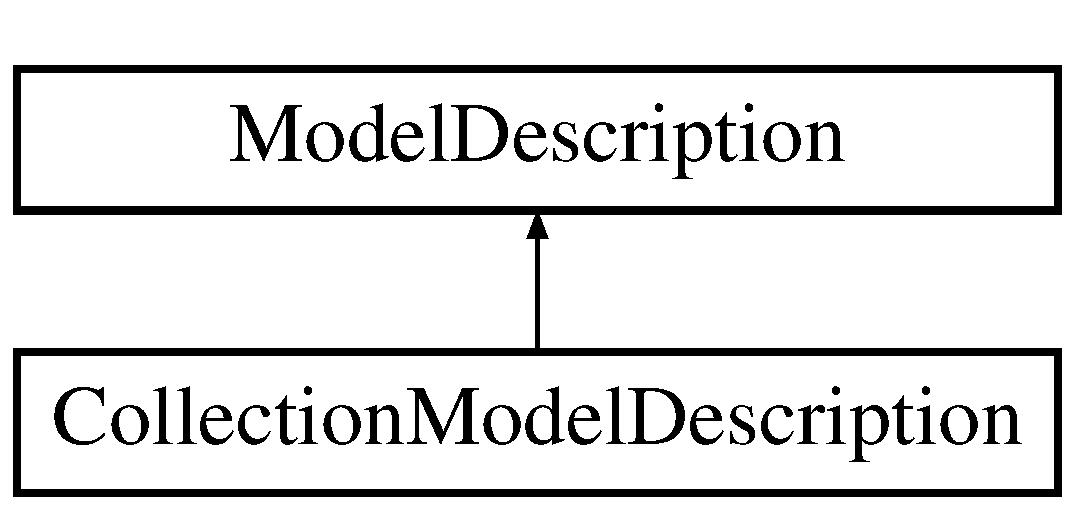
\includegraphics[height=2.000000cm]{d5/dbc/classApi3Layers_1_1Areas_1_1HelpPage_1_1ModelDescriptions_1_1CollectionModelDescription}
\end{center}
\end{figure}
\subsection*{Propriedades}
\begin{DoxyCompactItemize}
\item 
\hyperlink{classApi3Layers_1_1Areas_1_1HelpPage_1_1ModelDescriptions_1_1ModelDescription}{Model\+Description} \hyperlink{classApi3Layers_1_1Areas_1_1HelpPage_1_1ModelDescriptions_1_1CollectionModelDescription_a631f3e871530b1038022867696e8c7a9}{Element\+Description}\hspace{0.3cm}{\ttfamily  \mbox{[}get, set\mbox{]}}
\end{DoxyCompactItemize}


\subsection{Propriedades}
\mbox{\Hypertarget{classApi3Layers_1_1Areas_1_1HelpPage_1_1ModelDescriptions_1_1CollectionModelDescription_a631f3e871530b1038022867696e8c7a9}\label{classApi3Layers_1_1Areas_1_1HelpPage_1_1ModelDescriptions_1_1CollectionModelDescription_a631f3e871530b1038022867696e8c7a9}} 
\index{Api3\+Layers\+::\+Areas\+::\+Help\+Page\+::\+Model\+Descriptions\+::\+Collection\+Model\+Description@{Api3\+Layers\+::\+Areas\+::\+Help\+Page\+::\+Model\+Descriptions\+::\+Collection\+Model\+Description}!Element\+Description@{Element\+Description}}
\index{Element\+Description@{Element\+Description}!Api3\+Layers\+::\+Areas\+::\+Help\+Page\+::\+Model\+Descriptions\+::\+Collection\+Model\+Description@{Api3\+Layers\+::\+Areas\+::\+Help\+Page\+::\+Model\+Descriptions\+::\+Collection\+Model\+Description}}
\subsubsection{\texorpdfstring{Element\+Description}{ElementDescription}}
{\footnotesize\ttfamily \hyperlink{classApi3Layers_1_1Areas_1_1HelpPage_1_1ModelDescriptions_1_1ModelDescription}{Model\+Description} Element\+Description\hspace{0.3cm}{\ttfamily [get]}, {\ttfamily [set]}}



A documentação para esta classe foi gerada a partir do seguinte arquivo\+:\begin{DoxyCompactItemize}
\item 
C\+:/\+Users/\+Bruno/\+Desktop/\+Api3\+Layers/\+Api3\+Layers/\+Areas/\+Help\+Page/\+Model\+Descriptions/\hyperlink{CollectionModelDescription_8cs}{Collection\+Model\+Description.\+cs}\end{DoxyCompactItemize}

\hypertarget{classApi3Layers_1_1Areas_1_1HelpPage_1_1ModelDescriptions_1_1ComplexTypeModelDescription}{}\section{Complex\+Type\+Model\+Description}
\label{classApi3Layers_1_1Areas_1_1HelpPage_1_1ModelDescriptions_1_1ComplexTypeModelDescription}\index{Complex\+Type\+Model\+Description@{Complex\+Type\+Model\+Description}}
Diagrama de Hierarquia para Complex\+Type\+Model\+Description\+:\begin{figure}[H]
\begin{center}
\leavevmode
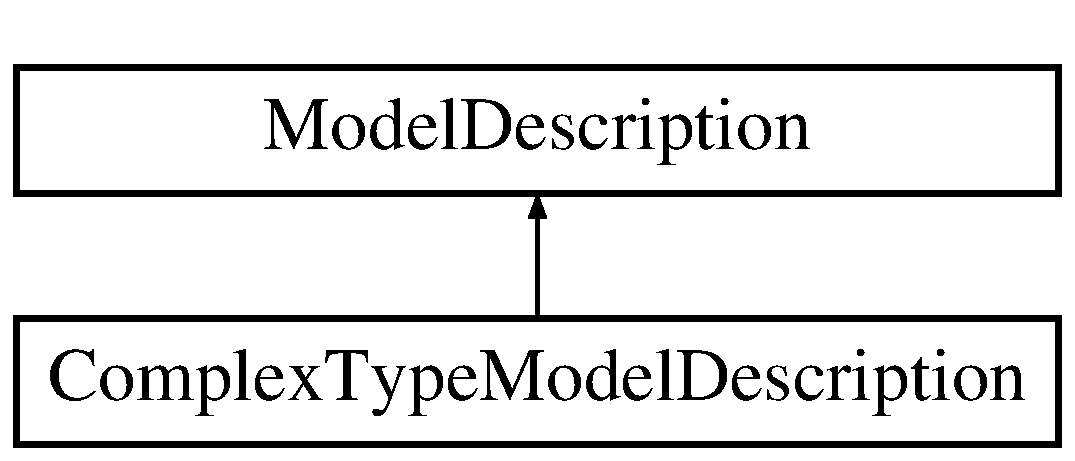
\includegraphics[height=2.000000cm]{classApi3Layers_1_1Areas_1_1HelpPage_1_1ModelDescriptions_1_1ComplexTypeModelDescription}
\end{center}
\end{figure}
\subsection*{Métodos Públicos}
\begin{DoxyCompactItemize}
\item 
\hyperlink{classApi3Layers_1_1Areas_1_1HelpPage_1_1ModelDescriptions_1_1ComplexTypeModelDescription_a81a0cc465616fd3a2f00f1295fafcb78}{Complex\+Type\+Model\+Description} ()
\end{DoxyCompactItemize}
\subsection*{Propriedades}
\begin{DoxyCompactItemize}
\item 
Collection$<$ \hyperlink{classApi3Layers_1_1Areas_1_1HelpPage_1_1ModelDescriptions_1_1ParameterDescription}{Parameter\+Description} $>$ \hyperlink{classApi3Layers_1_1Areas_1_1HelpPage_1_1ModelDescriptions_1_1ComplexTypeModelDescription_adc2966acc96bfe491b21fec063855b8c}{Properties}\hspace{0.3cm}{\ttfamily  \mbox{[}get, private set\mbox{]}}
\end{DoxyCompactItemize}


\subsection{Construtores \& Destrutores}
\mbox{\Hypertarget{classApi3Layers_1_1Areas_1_1HelpPage_1_1ModelDescriptions_1_1ComplexTypeModelDescription_a81a0cc465616fd3a2f00f1295fafcb78}\label{classApi3Layers_1_1Areas_1_1HelpPage_1_1ModelDescriptions_1_1ComplexTypeModelDescription_a81a0cc465616fd3a2f00f1295fafcb78}} 
\index{Api3\+Layers\+::\+Areas\+::\+Help\+Page\+::\+Model\+Descriptions\+::\+Complex\+Type\+Model\+Description@{Api3\+Layers\+::\+Areas\+::\+Help\+Page\+::\+Model\+Descriptions\+::\+Complex\+Type\+Model\+Description}!Complex\+Type\+Model\+Description@{Complex\+Type\+Model\+Description}}
\index{Complex\+Type\+Model\+Description@{Complex\+Type\+Model\+Description}!Api3\+Layers\+::\+Areas\+::\+Help\+Page\+::\+Model\+Descriptions\+::\+Complex\+Type\+Model\+Description@{Api3\+Layers\+::\+Areas\+::\+Help\+Page\+::\+Model\+Descriptions\+::\+Complex\+Type\+Model\+Description}}
\subsubsection{\texorpdfstring{Complex\+Type\+Model\+Description()}{ComplexTypeModelDescription()}}
{\footnotesize\ttfamily \hyperlink{classApi3Layers_1_1Areas_1_1HelpPage_1_1ModelDescriptions_1_1ComplexTypeModelDescription}{Complex\+Type\+Model\+Description} (\begin{DoxyParamCaption}{ }\end{DoxyParamCaption})}



\subsection{Propriedades}
\mbox{\Hypertarget{classApi3Layers_1_1Areas_1_1HelpPage_1_1ModelDescriptions_1_1ComplexTypeModelDescription_adc2966acc96bfe491b21fec063855b8c}\label{classApi3Layers_1_1Areas_1_1HelpPage_1_1ModelDescriptions_1_1ComplexTypeModelDescription_adc2966acc96bfe491b21fec063855b8c}} 
\index{Api3\+Layers\+::\+Areas\+::\+Help\+Page\+::\+Model\+Descriptions\+::\+Complex\+Type\+Model\+Description@{Api3\+Layers\+::\+Areas\+::\+Help\+Page\+::\+Model\+Descriptions\+::\+Complex\+Type\+Model\+Description}!Properties@{Properties}}
\index{Properties@{Properties}!Api3\+Layers\+::\+Areas\+::\+Help\+Page\+::\+Model\+Descriptions\+::\+Complex\+Type\+Model\+Description@{Api3\+Layers\+::\+Areas\+::\+Help\+Page\+::\+Model\+Descriptions\+::\+Complex\+Type\+Model\+Description}}
\subsubsection{\texorpdfstring{Properties}{Properties}}
{\footnotesize\ttfamily Collection$<$\hyperlink{classApi3Layers_1_1Areas_1_1HelpPage_1_1ModelDescriptions_1_1ParameterDescription}{Parameter\+Description}$>$ Properties\hspace{0.3cm}{\ttfamily [get]}, {\ttfamily [private set]}}



A documentação para esta classe foi gerada a partir do seguinte arquivo\+:\begin{DoxyCompactItemize}
\item 
Api3\+Layers/\+Areas/\+Help\+Page/\+Model\+Descriptions/\hyperlink{ComplexTypeModelDescription_8cs}{Complex\+Type\+Model\+Description.\+cs}\end{DoxyCompactItemize}

\hypertarget{classApi3Layers_1_1Areas_1_1HelpPage_1_1ModelDescriptions_1_1DictionaryModelDescription}{}\section{Dictionary\+Model\+Description}
\label{classApi3Layers_1_1Areas_1_1HelpPage_1_1ModelDescriptions_1_1DictionaryModelDescription}\index{Dictionary\+Model\+Description@{Dictionary\+Model\+Description}}
Diagrama de Hierarquia para Dictionary\+Model\+Description\+:\begin{figure}[H]
\begin{center}
\leavevmode
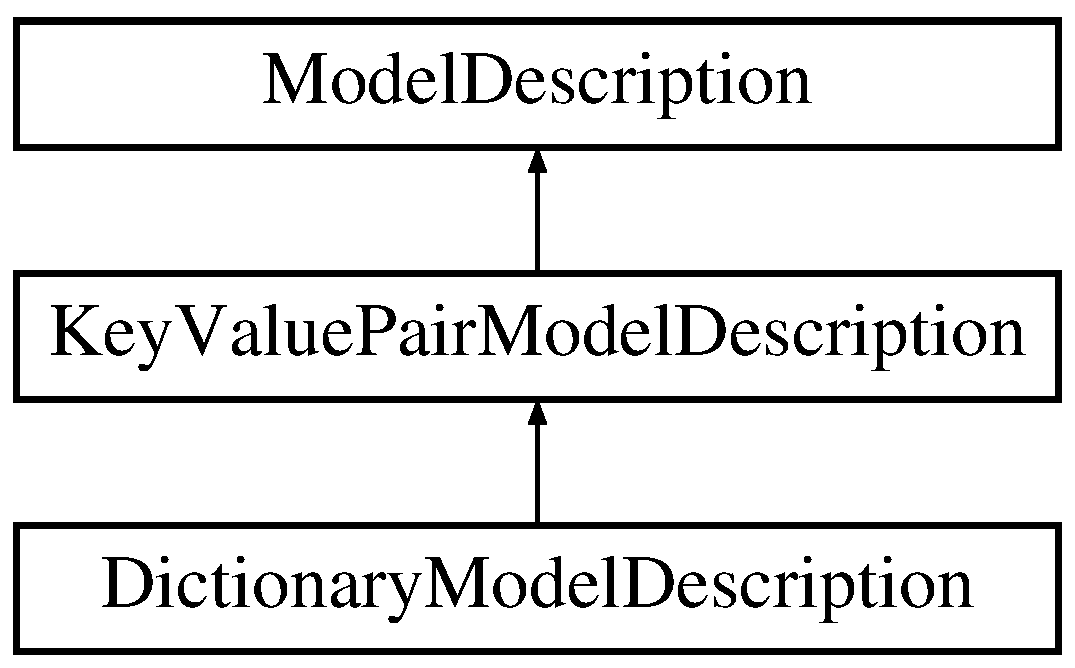
\includegraphics[height=3.000000cm]{classApi3Layers_1_1Areas_1_1HelpPage_1_1ModelDescriptions_1_1DictionaryModelDescription}
\end{center}
\end{figure}
\subsection*{Outros membros herdados}


A documentação para esta classe foi gerada a partir do seguinte arquivo\+:\begin{DoxyCompactItemize}
\item 
Api3\+Layers/\+Areas/\+Help\+Page/\+Model\+Descriptions/\hyperlink{DictionaryModelDescription_8cs}{Dictionary\+Model\+Description.\+cs}\end{DoxyCompactItemize}

\hypertarget{classApi3Layers_1_1Areas_1_1HelpPage_1_1ModelDescriptions_1_1EnumTypeModelDescription}{}\section{Enum\+Type\+Model\+Description}
\label{classApi3Layers_1_1Areas_1_1HelpPage_1_1ModelDescriptions_1_1EnumTypeModelDescription}\index{Enum\+Type\+Model\+Description@{Enum\+Type\+Model\+Description}}
Diagrama de Hierarquia para Enum\+Type\+Model\+Description\+:\begin{figure}[H]
\begin{center}
\leavevmode
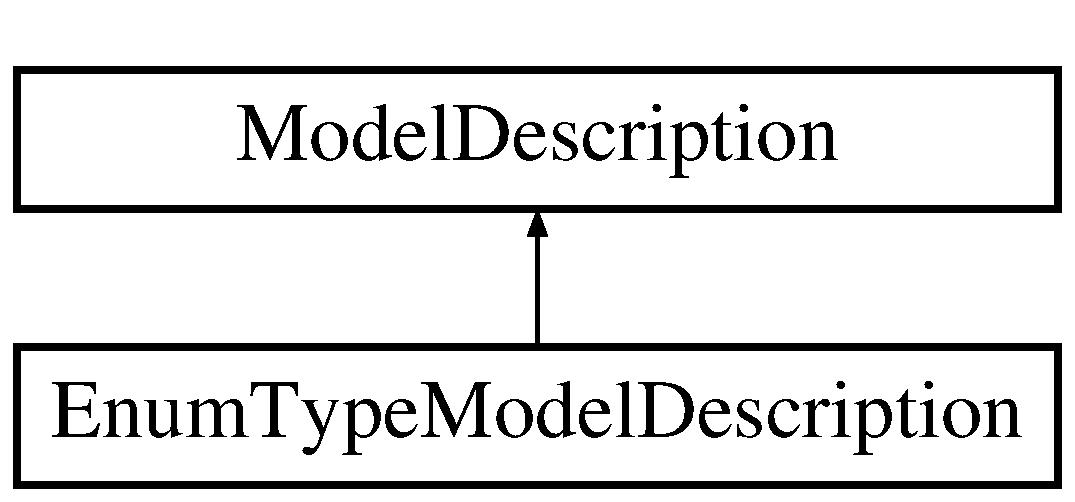
\includegraphics[height=2.000000cm]{d3/d68/classApi3Layers_1_1Areas_1_1HelpPage_1_1ModelDescriptions_1_1EnumTypeModelDescription}
\end{center}
\end{figure}
\subsection*{Métodos Públicos}
\begin{DoxyCompactItemize}
\item 
\hyperlink{classApi3Layers_1_1Areas_1_1HelpPage_1_1ModelDescriptions_1_1EnumTypeModelDescription_aab56d4e1f9f95ea7cc99ae3b97f3d4ba}{Enum\+Type\+Model\+Description} ()
\end{DoxyCompactItemize}
\subsection*{Propriedades}
\begin{DoxyCompactItemize}
\item 
Collection$<$ \hyperlink{classApi3Layers_1_1Areas_1_1HelpPage_1_1ModelDescriptions_1_1EnumValueDescription}{Enum\+Value\+Description} $>$ \hyperlink{classApi3Layers_1_1Areas_1_1HelpPage_1_1ModelDescriptions_1_1EnumTypeModelDescription_a4ca976ae041bc461662fd30b56fee02e}{Values}\hspace{0.3cm}{\ttfamily  \mbox{[}get, private set\mbox{]}}
\end{DoxyCompactItemize}


\subsection{Construtores \& Destrutores}
\mbox{\Hypertarget{classApi3Layers_1_1Areas_1_1HelpPage_1_1ModelDescriptions_1_1EnumTypeModelDescription_aab56d4e1f9f95ea7cc99ae3b97f3d4ba}\label{classApi3Layers_1_1Areas_1_1HelpPage_1_1ModelDescriptions_1_1EnumTypeModelDescription_aab56d4e1f9f95ea7cc99ae3b97f3d4ba}} 
\index{Api3\+Layers\+::\+Areas\+::\+Help\+Page\+::\+Model\+Descriptions\+::\+Enum\+Type\+Model\+Description@{Api3\+Layers\+::\+Areas\+::\+Help\+Page\+::\+Model\+Descriptions\+::\+Enum\+Type\+Model\+Description}!Enum\+Type\+Model\+Description@{Enum\+Type\+Model\+Description}}
\index{Enum\+Type\+Model\+Description@{Enum\+Type\+Model\+Description}!Api3\+Layers\+::\+Areas\+::\+Help\+Page\+::\+Model\+Descriptions\+::\+Enum\+Type\+Model\+Description@{Api3\+Layers\+::\+Areas\+::\+Help\+Page\+::\+Model\+Descriptions\+::\+Enum\+Type\+Model\+Description}}
\subsubsection{\texorpdfstring{Enum\+Type\+Model\+Description()}{EnumTypeModelDescription()}}
{\footnotesize\ttfamily \hyperlink{classApi3Layers_1_1Areas_1_1HelpPage_1_1ModelDescriptions_1_1EnumTypeModelDescription}{Enum\+Type\+Model\+Description} (\begin{DoxyParamCaption}{ }\end{DoxyParamCaption})}



\subsection{Propriedades}
\mbox{\Hypertarget{classApi3Layers_1_1Areas_1_1HelpPage_1_1ModelDescriptions_1_1EnumTypeModelDescription_a4ca976ae041bc461662fd30b56fee02e}\label{classApi3Layers_1_1Areas_1_1HelpPage_1_1ModelDescriptions_1_1EnumTypeModelDescription_a4ca976ae041bc461662fd30b56fee02e}} 
\index{Api3\+Layers\+::\+Areas\+::\+Help\+Page\+::\+Model\+Descriptions\+::\+Enum\+Type\+Model\+Description@{Api3\+Layers\+::\+Areas\+::\+Help\+Page\+::\+Model\+Descriptions\+::\+Enum\+Type\+Model\+Description}!Values@{Values}}
\index{Values@{Values}!Api3\+Layers\+::\+Areas\+::\+Help\+Page\+::\+Model\+Descriptions\+::\+Enum\+Type\+Model\+Description@{Api3\+Layers\+::\+Areas\+::\+Help\+Page\+::\+Model\+Descriptions\+::\+Enum\+Type\+Model\+Description}}
\subsubsection{\texorpdfstring{Values}{Values}}
{\footnotesize\ttfamily Collection$<$\hyperlink{classApi3Layers_1_1Areas_1_1HelpPage_1_1ModelDescriptions_1_1EnumValueDescription}{Enum\+Value\+Description}$>$ Values\hspace{0.3cm}{\ttfamily [get]}, {\ttfamily [private set]}}



A documentação para esta classe foi gerada a partir do seguinte arquivo\+:\begin{DoxyCompactItemize}
\item 
C\+:/\+Users/\+Bruno/\+Desktop/\+Api3\+Layers/\+Api3\+Layers/\+Areas/\+Help\+Page/\+Model\+Descriptions/\hyperlink{EnumTypeModelDescription_8cs}{Enum\+Type\+Model\+Description.\+cs}\end{DoxyCompactItemize}

\hypertarget{classApi3Layers_1_1Areas_1_1HelpPage_1_1ModelDescriptions_1_1EnumValueDescription}{}\section{Enum\+Value\+Description}
\label{classApi3Layers_1_1Areas_1_1HelpPage_1_1ModelDescriptions_1_1EnumValueDescription}\index{Enum\+Value\+Description@{Enum\+Value\+Description}}
\subsection*{Propriedades}
\begin{DoxyCompactItemize}
\item 
string \hyperlink{classApi3Layers_1_1Areas_1_1HelpPage_1_1ModelDescriptions_1_1EnumValueDescription_a239e2715951fcab2d9b263ef6acfa899}{Documentation}\hspace{0.3cm}{\ttfamily  \mbox{[}get, set\mbox{]}}
\item 
string \hyperlink{classApi3Layers_1_1Areas_1_1HelpPage_1_1ModelDescriptions_1_1EnumValueDescription_a7ee9065718e6628dc7791b756fa6c0f9}{Name}\hspace{0.3cm}{\ttfamily  \mbox{[}get, set\mbox{]}}
\item 
string \hyperlink{classApi3Layers_1_1Areas_1_1HelpPage_1_1ModelDescriptions_1_1EnumValueDescription_af7b88db799d8f791f785e437bc6099d2}{Value}\hspace{0.3cm}{\ttfamily  \mbox{[}get, set\mbox{]}}
\end{DoxyCompactItemize}


\subsection{Propriedades}
\mbox{\Hypertarget{classApi3Layers_1_1Areas_1_1HelpPage_1_1ModelDescriptions_1_1EnumValueDescription_a239e2715951fcab2d9b263ef6acfa899}\label{classApi3Layers_1_1Areas_1_1HelpPage_1_1ModelDescriptions_1_1EnumValueDescription_a239e2715951fcab2d9b263ef6acfa899}} 
\index{Api3\+Layers\+::\+Areas\+::\+Help\+Page\+::\+Model\+Descriptions\+::\+Enum\+Value\+Description@{Api3\+Layers\+::\+Areas\+::\+Help\+Page\+::\+Model\+Descriptions\+::\+Enum\+Value\+Description}!Documentation@{Documentation}}
\index{Documentation@{Documentation}!Api3\+Layers\+::\+Areas\+::\+Help\+Page\+::\+Model\+Descriptions\+::\+Enum\+Value\+Description@{Api3\+Layers\+::\+Areas\+::\+Help\+Page\+::\+Model\+Descriptions\+::\+Enum\+Value\+Description}}
\subsubsection{\texorpdfstring{Documentation}{Documentation}}
{\footnotesize\ttfamily string Documentation\hspace{0.3cm}{\ttfamily [get]}, {\ttfamily [set]}}

\mbox{\Hypertarget{classApi3Layers_1_1Areas_1_1HelpPage_1_1ModelDescriptions_1_1EnumValueDescription_a7ee9065718e6628dc7791b756fa6c0f9}\label{classApi3Layers_1_1Areas_1_1HelpPage_1_1ModelDescriptions_1_1EnumValueDescription_a7ee9065718e6628dc7791b756fa6c0f9}} 
\index{Api3\+Layers\+::\+Areas\+::\+Help\+Page\+::\+Model\+Descriptions\+::\+Enum\+Value\+Description@{Api3\+Layers\+::\+Areas\+::\+Help\+Page\+::\+Model\+Descriptions\+::\+Enum\+Value\+Description}!Name@{Name}}
\index{Name@{Name}!Api3\+Layers\+::\+Areas\+::\+Help\+Page\+::\+Model\+Descriptions\+::\+Enum\+Value\+Description@{Api3\+Layers\+::\+Areas\+::\+Help\+Page\+::\+Model\+Descriptions\+::\+Enum\+Value\+Description}}
\subsubsection{\texorpdfstring{Name}{Name}}
{\footnotesize\ttfamily string Name\hspace{0.3cm}{\ttfamily [get]}, {\ttfamily [set]}}

\mbox{\Hypertarget{classApi3Layers_1_1Areas_1_1HelpPage_1_1ModelDescriptions_1_1EnumValueDescription_af7b88db799d8f791f785e437bc6099d2}\label{classApi3Layers_1_1Areas_1_1HelpPage_1_1ModelDescriptions_1_1EnumValueDescription_af7b88db799d8f791f785e437bc6099d2}} 
\index{Api3\+Layers\+::\+Areas\+::\+Help\+Page\+::\+Model\+Descriptions\+::\+Enum\+Value\+Description@{Api3\+Layers\+::\+Areas\+::\+Help\+Page\+::\+Model\+Descriptions\+::\+Enum\+Value\+Description}!Value@{Value}}
\index{Value@{Value}!Api3\+Layers\+::\+Areas\+::\+Help\+Page\+::\+Model\+Descriptions\+::\+Enum\+Value\+Description@{Api3\+Layers\+::\+Areas\+::\+Help\+Page\+::\+Model\+Descriptions\+::\+Enum\+Value\+Description}}
\subsubsection{\texorpdfstring{Value}{Value}}
{\footnotesize\ttfamily string Value\hspace{0.3cm}{\ttfamily [get]}, {\ttfamily [set]}}



A documentação para esta classe foi gerada a partir do seguinte arquivo\+:\begin{DoxyCompactItemize}
\item 
C\+:/\+Users/\+Bruno/\+Desktop/\+Api3\+Layers/\+Api3\+Layers/\+Areas/\+Help\+Page/\+Model\+Descriptions/\hyperlink{EnumValueDescription_8cs}{Enum\+Value\+Description.\+cs}\end{DoxyCompactItemize}

\hypertarget{interfaceApi3Layers_1_1Areas_1_1HelpPage_1_1ModelDescriptions_1_1IModelDocumentationProvider}{}\section{I\+Model\+Documentation\+Provider}
\label{interfaceApi3Layers_1_1Areas_1_1HelpPage_1_1ModelDescriptions_1_1IModelDocumentationProvider}\index{I\+Model\+Documentation\+Provider@{I\+Model\+Documentation\+Provider}}
Diagrama de Hierarquia para I\+Model\+Documentation\+Provider\+:\begin{figure}[H]
\begin{center}
\leavevmode
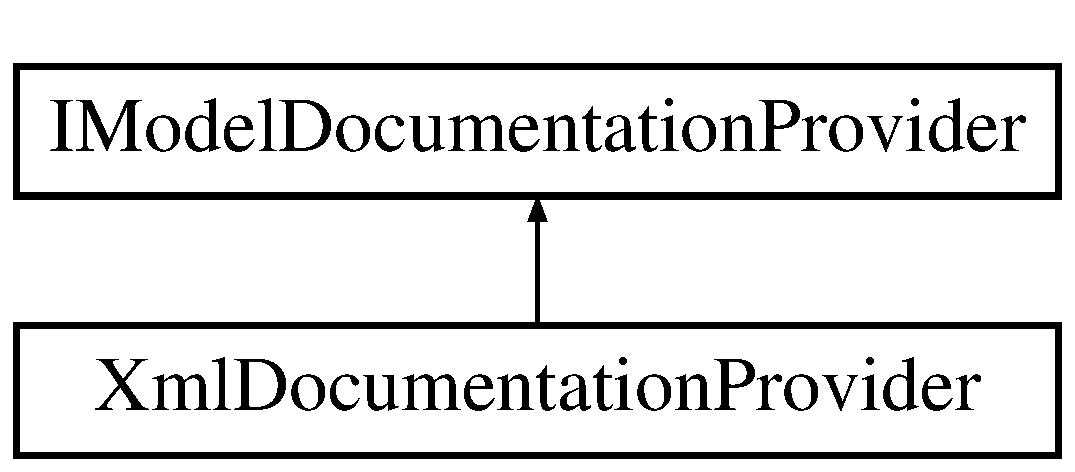
\includegraphics[height=2.000000cm]{interfaceApi3Layers_1_1Areas_1_1HelpPage_1_1ModelDescriptions_1_1IModelDocumentationProvider}
\end{center}
\end{figure}
\subsection*{Métodos Públicos}
\begin{DoxyCompactItemize}
\item 
string \hyperlink{interfaceApi3Layers_1_1Areas_1_1HelpPage_1_1ModelDescriptions_1_1IModelDocumentationProvider_aa774bb352a769421583abb335a1cec8a}{Get\+Documentation} (Member\+Info member)
\item 
string \hyperlink{interfaceApi3Layers_1_1Areas_1_1HelpPage_1_1ModelDescriptions_1_1IModelDocumentationProvider_af771cd863288942e506d28447daf4f82}{Get\+Documentation} (Type type)
\end{DoxyCompactItemize}


\subsection{Métodos}
\mbox{\Hypertarget{interfaceApi3Layers_1_1Areas_1_1HelpPage_1_1ModelDescriptions_1_1IModelDocumentationProvider_aa774bb352a769421583abb335a1cec8a}\label{interfaceApi3Layers_1_1Areas_1_1HelpPage_1_1ModelDescriptions_1_1IModelDocumentationProvider_aa774bb352a769421583abb335a1cec8a}} 
\index{Api3\+Layers\+::\+Areas\+::\+Help\+Page\+::\+Model\+Descriptions\+::\+I\+Model\+Documentation\+Provider@{Api3\+Layers\+::\+Areas\+::\+Help\+Page\+::\+Model\+Descriptions\+::\+I\+Model\+Documentation\+Provider}!Get\+Documentation@{Get\+Documentation}}
\index{Get\+Documentation@{Get\+Documentation}!Api3\+Layers\+::\+Areas\+::\+Help\+Page\+::\+Model\+Descriptions\+::\+I\+Model\+Documentation\+Provider@{Api3\+Layers\+::\+Areas\+::\+Help\+Page\+::\+Model\+Descriptions\+::\+I\+Model\+Documentation\+Provider}}
\subsubsection{\texorpdfstring{Get\+Documentation()}{GetDocumentation()}\hspace{0.1cm}{\footnotesize\ttfamily [1/2]}}
{\footnotesize\ttfamily string Get\+Documentation (\begin{DoxyParamCaption}\item[{Member\+Info}]{member }\end{DoxyParamCaption})}



Implementado por \hyperlink{classApi3Layers_1_1Areas_1_1HelpPage_1_1XmlDocumentationProvider_aa774bb352a769421583abb335a1cec8a}{Xml\+Documentation\+Provider}.

\mbox{\Hypertarget{interfaceApi3Layers_1_1Areas_1_1HelpPage_1_1ModelDescriptions_1_1IModelDocumentationProvider_af771cd863288942e506d28447daf4f82}\label{interfaceApi3Layers_1_1Areas_1_1HelpPage_1_1ModelDescriptions_1_1IModelDocumentationProvider_af771cd863288942e506d28447daf4f82}} 
\index{Api3\+Layers\+::\+Areas\+::\+Help\+Page\+::\+Model\+Descriptions\+::\+I\+Model\+Documentation\+Provider@{Api3\+Layers\+::\+Areas\+::\+Help\+Page\+::\+Model\+Descriptions\+::\+I\+Model\+Documentation\+Provider}!Get\+Documentation@{Get\+Documentation}}
\index{Get\+Documentation@{Get\+Documentation}!Api3\+Layers\+::\+Areas\+::\+Help\+Page\+::\+Model\+Descriptions\+::\+I\+Model\+Documentation\+Provider@{Api3\+Layers\+::\+Areas\+::\+Help\+Page\+::\+Model\+Descriptions\+::\+I\+Model\+Documentation\+Provider}}
\subsubsection{\texorpdfstring{Get\+Documentation()}{GetDocumentation()}\hspace{0.1cm}{\footnotesize\ttfamily [2/2]}}
{\footnotesize\ttfamily string Get\+Documentation (\begin{DoxyParamCaption}\item[{Type}]{type }\end{DoxyParamCaption})}



Implementado por \hyperlink{classApi3Layers_1_1Areas_1_1HelpPage_1_1XmlDocumentationProvider_af771cd863288942e506d28447daf4f82}{Xml\+Documentation\+Provider}.



A documentação para esta interface foi gerada a partir do seguinte arquivo\+:\begin{DoxyCompactItemize}
\item 
Api3\+Layers/\+Areas/\+Help\+Page/\+Model\+Descriptions/\hyperlink{IModelDocumentationProvider_8cs}{I\+Model\+Documentation\+Provider.\+cs}\end{DoxyCompactItemize}

\hypertarget{classApi3Layers_1_1Areas_1_1HelpPage_1_1ModelDescriptions_1_1KeyValuePairModelDescription}{}\section{Key\+Value\+Pair\+Model\+Description}
\label{classApi3Layers_1_1Areas_1_1HelpPage_1_1ModelDescriptions_1_1KeyValuePairModelDescription}\index{Key\+Value\+Pair\+Model\+Description@{Key\+Value\+Pair\+Model\+Description}}
Diagrama de Hierarquia para Key\+Value\+Pair\+Model\+Description\+:\begin{figure}[H]
\begin{center}
\leavevmode
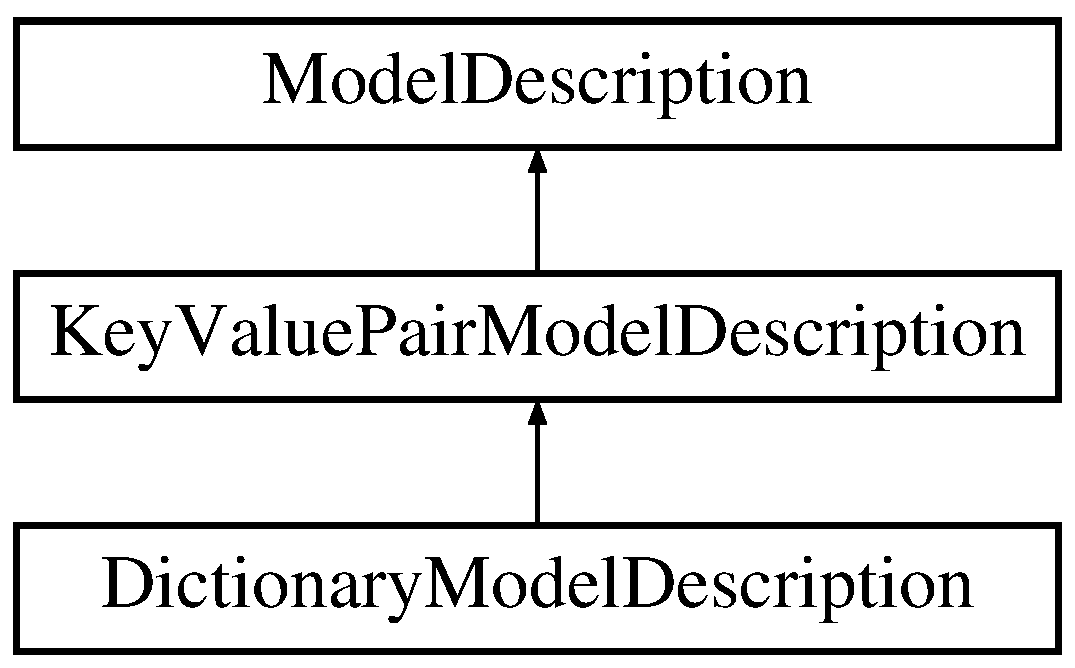
\includegraphics[height=3.000000cm]{dd/d36/classApi3Layers_1_1Areas_1_1HelpPage_1_1ModelDescriptions_1_1KeyValuePairModelDescription}
\end{center}
\end{figure}
\subsection*{Propriedades}
\begin{DoxyCompactItemize}
\item 
\hyperlink{classApi3Layers_1_1Areas_1_1HelpPage_1_1ModelDescriptions_1_1ModelDescription}{Model\+Description} \hyperlink{classApi3Layers_1_1Areas_1_1HelpPage_1_1ModelDescriptions_1_1KeyValuePairModelDescription_a007c899d0967cadd0ba3dd3401b835ea}{Key\+Model\+Description}\hspace{0.3cm}{\ttfamily  \mbox{[}get, set\mbox{]}}
\item 
\hyperlink{classApi3Layers_1_1Areas_1_1HelpPage_1_1ModelDescriptions_1_1ModelDescription}{Model\+Description} \hyperlink{classApi3Layers_1_1Areas_1_1HelpPage_1_1ModelDescriptions_1_1KeyValuePairModelDescription_aa80f5630d332a9c35eea5c0f793574e5}{Value\+Model\+Description}\hspace{0.3cm}{\ttfamily  \mbox{[}get, set\mbox{]}}
\end{DoxyCompactItemize}


\subsection{Propriedades}
\mbox{\Hypertarget{classApi3Layers_1_1Areas_1_1HelpPage_1_1ModelDescriptions_1_1KeyValuePairModelDescription_a007c899d0967cadd0ba3dd3401b835ea}\label{classApi3Layers_1_1Areas_1_1HelpPage_1_1ModelDescriptions_1_1KeyValuePairModelDescription_a007c899d0967cadd0ba3dd3401b835ea}} 
\index{Api3\+Layers\+::\+Areas\+::\+Help\+Page\+::\+Model\+Descriptions\+::\+Key\+Value\+Pair\+Model\+Description@{Api3\+Layers\+::\+Areas\+::\+Help\+Page\+::\+Model\+Descriptions\+::\+Key\+Value\+Pair\+Model\+Description}!Key\+Model\+Description@{Key\+Model\+Description}}
\index{Key\+Model\+Description@{Key\+Model\+Description}!Api3\+Layers\+::\+Areas\+::\+Help\+Page\+::\+Model\+Descriptions\+::\+Key\+Value\+Pair\+Model\+Description@{Api3\+Layers\+::\+Areas\+::\+Help\+Page\+::\+Model\+Descriptions\+::\+Key\+Value\+Pair\+Model\+Description}}
\subsubsection{\texorpdfstring{Key\+Model\+Description}{KeyModelDescription}}
{\footnotesize\ttfamily \hyperlink{classApi3Layers_1_1Areas_1_1HelpPage_1_1ModelDescriptions_1_1ModelDescription}{Model\+Description} Key\+Model\+Description\hspace{0.3cm}{\ttfamily [get]}, {\ttfamily [set]}}

\mbox{\Hypertarget{classApi3Layers_1_1Areas_1_1HelpPage_1_1ModelDescriptions_1_1KeyValuePairModelDescription_aa80f5630d332a9c35eea5c0f793574e5}\label{classApi3Layers_1_1Areas_1_1HelpPage_1_1ModelDescriptions_1_1KeyValuePairModelDescription_aa80f5630d332a9c35eea5c0f793574e5}} 
\index{Api3\+Layers\+::\+Areas\+::\+Help\+Page\+::\+Model\+Descriptions\+::\+Key\+Value\+Pair\+Model\+Description@{Api3\+Layers\+::\+Areas\+::\+Help\+Page\+::\+Model\+Descriptions\+::\+Key\+Value\+Pair\+Model\+Description}!Value\+Model\+Description@{Value\+Model\+Description}}
\index{Value\+Model\+Description@{Value\+Model\+Description}!Api3\+Layers\+::\+Areas\+::\+Help\+Page\+::\+Model\+Descriptions\+::\+Key\+Value\+Pair\+Model\+Description@{Api3\+Layers\+::\+Areas\+::\+Help\+Page\+::\+Model\+Descriptions\+::\+Key\+Value\+Pair\+Model\+Description}}
\subsubsection{\texorpdfstring{Value\+Model\+Description}{ValueModelDescription}}
{\footnotesize\ttfamily \hyperlink{classApi3Layers_1_1Areas_1_1HelpPage_1_1ModelDescriptions_1_1ModelDescription}{Model\+Description} Value\+Model\+Description\hspace{0.3cm}{\ttfamily [get]}, {\ttfamily [set]}}



A documentação para esta classe foi gerada a partir do seguinte arquivo\+:\begin{DoxyCompactItemize}
\item 
C\+:/\+Users/\+Bruno/\+Desktop/\+Api3\+Layers/\+Api3\+Layers/\+Areas/\+Help\+Page/\+Model\+Descriptions/\hyperlink{KeyValuePairModelDescription_8cs}{Key\+Value\+Pair\+Model\+Description.\+cs}\end{DoxyCompactItemize}

\hypertarget{classApi3Layers_1_1Areas_1_1HelpPage_1_1ModelDescriptions_1_1ModelDescription}{}\section{Model\+Description}
\label{classApi3Layers_1_1Areas_1_1HelpPage_1_1ModelDescriptions_1_1ModelDescription}\index{Model\+Description@{Model\+Description}}


Describes a type model.  


Diagrama de Hierarquia para Model\+Description\+:\begin{figure}[H]
\begin{center}
\leavevmode
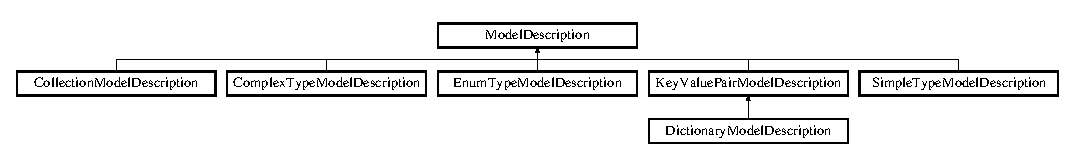
\includegraphics[height=1.705584cm]{classApi3Layers_1_1Areas_1_1HelpPage_1_1ModelDescriptions_1_1ModelDescription}
\end{center}
\end{figure}
\subsection*{Propriedades}
\begin{DoxyCompactItemize}
\item 
string \hyperlink{classApi3Layers_1_1Areas_1_1HelpPage_1_1ModelDescriptions_1_1ModelDescription_a239e2715951fcab2d9b263ef6acfa899}{Documentation}\hspace{0.3cm}{\ttfamily  \mbox{[}get, set\mbox{]}}
\item 
Type \hyperlink{classApi3Layers_1_1Areas_1_1HelpPage_1_1ModelDescriptions_1_1ModelDescription_ab4e6bdc2197fcee901bb151c8d9fa3c2}{Model\+Type}\hspace{0.3cm}{\ttfamily  \mbox{[}get, set\mbox{]}}
\item 
string \hyperlink{classApi3Layers_1_1Areas_1_1HelpPage_1_1ModelDescriptions_1_1ModelDescription_a7ee9065718e6628dc7791b756fa6c0f9}{Name}\hspace{0.3cm}{\ttfamily  \mbox{[}get, set\mbox{]}}
\end{DoxyCompactItemize}


\subsection{Descrição Detalhada}
Describes a type model. 



\subsection{Propriedades}
\mbox{\Hypertarget{classApi3Layers_1_1Areas_1_1HelpPage_1_1ModelDescriptions_1_1ModelDescription_a239e2715951fcab2d9b263ef6acfa899}\label{classApi3Layers_1_1Areas_1_1HelpPage_1_1ModelDescriptions_1_1ModelDescription_a239e2715951fcab2d9b263ef6acfa899}} 
\index{Api3\+Layers\+::\+Areas\+::\+Help\+Page\+::\+Model\+Descriptions\+::\+Model\+Description@{Api3\+Layers\+::\+Areas\+::\+Help\+Page\+::\+Model\+Descriptions\+::\+Model\+Description}!Documentation@{Documentation}}
\index{Documentation@{Documentation}!Api3\+Layers\+::\+Areas\+::\+Help\+Page\+::\+Model\+Descriptions\+::\+Model\+Description@{Api3\+Layers\+::\+Areas\+::\+Help\+Page\+::\+Model\+Descriptions\+::\+Model\+Description}}
\subsubsection{\texorpdfstring{Documentation}{Documentation}}
{\footnotesize\ttfamily string Documentation\hspace{0.3cm}{\ttfamily [get]}, {\ttfamily [set]}}

\mbox{\Hypertarget{classApi3Layers_1_1Areas_1_1HelpPage_1_1ModelDescriptions_1_1ModelDescription_ab4e6bdc2197fcee901bb151c8d9fa3c2}\label{classApi3Layers_1_1Areas_1_1HelpPage_1_1ModelDescriptions_1_1ModelDescription_ab4e6bdc2197fcee901bb151c8d9fa3c2}} 
\index{Api3\+Layers\+::\+Areas\+::\+Help\+Page\+::\+Model\+Descriptions\+::\+Model\+Description@{Api3\+Layers\+::\+Areas\+::\+Help\+Page\+::\+Model\+Descriptions\+::\+Model\+Description}!Model\+Type@{Model\+Type}}
\index{Model\+Type@{Model\+Type}!Api3\+Layers\+::\+Areas\+::\+Help\+Page\+::\+Model\+Descriptions\+::\+Model\+Description@{Api3\+Layers\+::\+Areas\+::\+Help\+Page\+::\+Model\+Descriptions\+::\+Model\+Description}}
\subsubsection{\texorpdfstring{Model\+Type}{ModelType}}
{\footnotesize\ttfamily Type Model\+Type\hspace{0.3cm}{\ttfamily [get]}, {\ttfamily [set]}}

\mbox{\Hypertarget{classApi3Layers_1_1Areas_1_1HelpPage_1_1ModelDescriptions_1_1ModelDescription_a7ee9065718e6628dc7791b756fa6c0f9}\label{classApi3Layers_1_1Areas_1_1HelpPage_1_1ModelDescriptions_1_1ModelDescription_a7ee9065718e6628dc7791b756fa6c0f9}} 
\index{Api3\+Layers\+::\+Areas\+::\+Help\+Page\+::\+Model\+Descriptions\+::\+Model\+Description@{Api3\+Layers\+::\+Areas\+::\+Help\+Page\+::\+Model\+Descriptions\+::\+Model\+Description}!Name@{Name}}
\index{Name@{Name}!Api3\+Layers\+::\+Areas\+::\+Help\+Page\+::\+Model\+Descriptions\+::\+Model\+Description@{Api3\+Layers\+::\+Areas\+::\+Help\+Page\+::\+Model\+Descriptions\+::\+Model\+Description}}
\subsubsection{\texorpdfstring{Name}{Name}}
{\footnotesize\ttfamily string Name\hspace{0.3cm}{\ttfamily [get]}, {\ttfamily [set]}}



A documentação para esta classe foi gerada a partir do seguinte arquivo\+:\begin{DoxyCompactItemize}
\item 
Api3\+Layers/\+Areas/\+Help\+Page/\+Model\+Descriptions/\hyperlink{ModelDescription_8cs}{Model\+Description.\+cs}\end{DoxyCompactItemize}

\hypertarget{classApi3Layers_1_1Areas_1_1HelpPage_1_1ModelDescriptions_1_1ModelDescriptionGenerator}{}\section{Model\+Description\+Generator}
\label{classApi3Layers_1_1Areas_1_1HelpPage_1_1ModelDescriptions_1_1ModelDescriptionGenerator}\index{Model\+Description\+Generator@{Model\+Description\+Generator}}


Generates model descriptions for given types.  


\subsection*{Métodos Públicos}
\begin{DoxyCompactItemize}
\item 
\hyperlink{classApi3Layers_1_1Areas_1_1HelpPage_1_1ModelDescriptions_1_1ModelDescriptionGenerator_a8bb9d53927e07e7e5a9e24cb692e52db}{Model\+Description\+Generator} (Http\+Configuration config)
\item 
\hyperlink{classApi3Layers_1_1Areas_1_1HelpPage_1_1ModelDescriptions_1_1ModelDescription}{Model\+Description} \hyperlink{classApi3Layers_1_1Areas_1_1HelpPage_1_1ModelDescriptions_1_1ModelDescriptionGenerator_ac19c99af386f86f13717a447e965f9d7}{Get\+Or\+Create\+Model\+Description} (Type model\+Type)
\end{DoxyCompactItemize}
\subsection*{Propriedades}
\begin{DoxyCompactItemize}
\item 
\hyperlink{interfaceApi3Layers_1_1Areas_1_1HelpPage_1_1ModelDescriptions_1_1IModelDocumentationProvider}{I\+Model\+Documentation\+Provider} \hyperlink{classApi3Layers_1_1Areas_1_1HelpPage_1_1ModelDescriptions_1_1ModelDescriptionGenerator_a4652be127f17b1d03648642fa509968c}{Documentation\+Provider}\hspace{0.3cm}{\ttfamily  \mbox{[}get\mbox{]}}
\item 
Dictionary$<$ string, \hyperlink{classApi3Layers_1_1Areas_1_1HelpPage_1_1ModelDescriptions_1_1ModelDescription}{Model\+Description} $>$ \hyperlink{classApi3Layers_1_1Areas_1_1HelpPage_1_1ModelDescriptions_1_1ModelDescriptionGenerator_a3132a32205bd0f5029c2a01ab8c29e64}{Generated\+Models}\hspace{0.3cm}{\ttfamily  \mbox{[}get, private set\mbox{]}}
\end{DoxyCompactItemize}
\subsection*{Métodos Privados}
\begin{DoxyCompactItemize}
\item 
string \hyperlink{classApi3Layers_1_1Areas_1_1HelpPage_1_1ModelDescriptions_1_1ModelDescriptionGenerator_a64f78a7390688c87d31a887a9836beb4}{Create\+Default\+Documentation} (Type type)
\item 
void \hyperlink{classApi3Layers_1_1Areas_1_1HelpPage_1_1ModelDescriptions_1_1ModelDescriptionGenerator_ac38e76f941bb03e6602ec01872eaaa47}{Generate\+Annotations} (Member\+Info property, \hyperlink{classApi3Layers_1_1Areas_1_1HelpPage_1_1ModelDescriptions_1_1ParameterDescription}{Parameter\+Description} property\+Model)
\item 
\hyperlink{classApi3Layers_1_1Areas_1_1HelpPage_1_1ModelDescriptions_1_1CollectionModelDescription}{Collection\+Model\+Description} \hyperlink{classApi3Layers_1_1Areas_1_1HelpPage_1_1ModelDescriptions_1_1ModelDescriptionGenerator_aa65206c5e43db1c9d4c375539496f72d}{Generate\+Collection\+Model\+Description} (Type model\+Type, Type element\+Type)
\item 
\hyperlink{classApi3Layers_1_1Areas_1_1HelpPage_1_1ModelDescriptions_1_1ModelDescription}{Model\+Description} \hyperlink{classApi3Layers_1_1Areas_1_1HelpPage_1_1ModelDescriptions_1_1ModelDescriptionGenerator_a3d6912f5ad147d7d6683fba5d473a0ef}{Generate\+Complex\+Type\+Model\+Description} (Type model\+Type)
\item 
\hyperlink{classApi3Layers_1_1Areas_1_1HelpPage_1_1ModelDescriptions_1_1DictionaryModelDescription}{Dictionary\+Model\+Description} \hyperlink{classApi3Layers_1_1Areas_1_1HelpPage_1_1ModelDescriptions_1_1ModelDescriptionGenerator_ad8bba1e2e53b9d38faea81ca34b9ce92}{Generate\+Dictionary\+Model\+Description} (Type model\+Type, Type key\+Type, Type value\+Type)
\item 
\hyperlink{classApi3Layers_1_1Areas_1_1HelpPage_1_1ModelDescriptions_1_1EnumTypeModelDescription}{Enum\+Type\+Model\+Description} \hyperlink{classApi3Layers_1_1Areas_1_1HelpPage_1_1ModelDescriptions_1_1ModelDescriptionGenerator_a109bbcef4577be599414712bd9c04418}{Generate\+Enum\+Type\+Model\+Description} (Type model\+Type)
\item 
\hyperlink{classApi3Layers_1_1Areas_1_1HelpPage_1_1ModelDescriptions_1_1KeyValuePairModelDescription}{Key\+Value\+Pair\+Model\+Description} \hyperlink{classApi3Layers_1_1Areas_1_1HelpPage_1_1ModelDescriptions_1_1ModelDescriptionGenerator_a529f7a95c1863412ca1613c3cece0dc8}{Generate\+Key\+Value\+Pair\+Model\+Description} (Type model\+Type, Type key\+Type, Type value\+Type)
\item 
\hyperlink{classApi3Layers_1_1Areas_1_1HelpPage_1_1ModelDescriptions_1_1ModelDescription}{Model\+Description} \hyperlink{classApi3Layers_1_1Areas_1_1HelpPage_1_1ModelDescriptions_1_1ModelDescriptionGenerator_aa450e2d5fb6e71f7e40805ce495b18ab}{Generate\+Simple\+Type\+Model\+Description} (Type model\+Type)
\end{DoxyCompactItemize}
\subsection*{Métodos Privados Estáticos}
\begin{DoxyCompactItemize}
\item 
static string \hyperlink{classApi3Layers_1_1Areas_1_1HelpPage_1_1ModelDescriptions_1_1ModelDescriptionGenerator_a268cc276ed084ff82617982818a8fc11}{Get\+Member\+Name} (Member\+Info member, bool has\+Data\+Contract\+Attribute)
\item 
static bool \hyperlink{classApi3Layers_1_1Areas_1_1HelpPage_1_1ModelDescriptions_1_1ModelDescriptionGenerator_a4002b466b6f40e9127162ccf3a2bd49d}{Should\+Display\+Member} (Member\+Info member, bool has\+Data\+Contract\+Attribute)
\end{DoxyCompactItemize}
\subsection*{Atributos Privados}
\begin{DoxyCompactItemize}
\item 
Lazy$<$ \hyperlink{interfaceApi3Layers_1_1Areas_1_1HelpPage_1_1ModelDescriptions_1_1IModelDocumentationProvider}{I\+Model\+Documentation\+Provider} $>$ \hyperlink{classApi3Layers_1_1Areas_1_1HelpPage_1_1ModelDescriptions_1_1ModelDescriptionGenerator_ac6c66f56f0e7953a9ca3d1b25394a922}{\+\_\+documentation\+Provider}
\item 
readonly I\+Dictionary$<$ Type, Func$<$ object, string $>$ $>$ \hyperlink{classApi3Layers_1_1Areas_1_1HelpPage_1_1ModelDescriptions_1_1ModelDescriptionGenerator_a8ff972f20473e943bcc5a435cd8921dc}{Annotation\+Text\+Generator}
\item 
readonly I\+Dictionary$<$ Type, string $>$ \hyperlink{classApi3Layers_1_1Areas_1_1HelpPage_1_1ModelDescriptions_1_1ModelDescriptionGenerator_a439e9d56d8dd09e116c825d3f0f6afe7}{Default\+Type\+Documentation}
\end{DoxyCompactItemize}


\subsection{Descrição Detalhada}
Generates model descriptions for given types. 



\subsection{Construtores \& Destrutores}
\mbox{\Hypertarget{classApi3Layers_1_1Areas_1_1HelpPage_1_1ModelDescriptions_1_1ModelDescriptionGenerator_a8bb9d53927e07e7e5a9e24cb692e52db}\label{classApi3Layers_1_1Areas_1_1HelpPage_1_1ModelDescriptions_1_1ModelDescriptionGenerator_a8bb9d53927e07e7e5a9e24cb692e52db}} 
\index{Api3\+Layers\+::\+Areas\+::\+Help\+Page\+::\+Model\+Descriptions\+::\+Model\+Description\+Generator@{Api3\+Layers\+::\+Areas\+::\+Help\+Page\+::\+Model\+Descriptions\+::\+Model\+Description\+Generator}!Model\+Description\+Generator@{Model\+Description\+Generator}}
\index{Model\+Description\+Generator@{Model\+Description\+Generator}!Api3\+Layers\+::\+Areas\+::\+Help\+Page\+::\+Model\+Descriptions\+::\+Model\+Description\+Generator@{Api3\+Layers\+::\+Areas\+::\+Help\+Page\+::\+Model\+Descriptions\+::\+Model\+Description\+Generator}}
\subsubsection{\texorpdfstring{Model\+Description\+Generator()}{ModelDescriptionGenerator()}}
{\footnotesize\ttfamily \hyperlink{classApi3Layers_1_1Areas_1_1HelpPage_1_1ModelDescriptions_1_1ModelDescriptionGenerator}{Model\+Description\+Generator} (\begin{DoxyParamCaption}\item[{Http\+Configuration}]{config }\end{DoxyParamCaption})}



\subsection{Métodos}
\mbox{\Hypertarget{classApi3Layers_1_1Areas_1_1HelpPage_1_1ModelDescriptions_1_1ModelDescriptionGenerator_a64f78a7390688c87d31a887a9836beb4}\label{classApi3Layers_1_1Areas_1_1HelpPage_1_1ModelDescriptions_1_1ModelDescriptionGenerator_a64f78a7390688c87d31a887a9836beb4}} 
\index{Api3\+Layers\+::\+Areas\+::\+Help\+Page\+::\+Model\+Descriptions\+::\+Model\+Description\+Generator@{Api3\+Layers\+::\+Areas\+::\+Help\+Page\+::\+Model\+Descriptions\+::\+Model\+Description\+Generator}!Create\+Default\+Documentation@{Create\+Default\+Documentation}}
\index{Create\+Default\+Documentation@{Create\+Default\+Documentation}!Api3\+Layers\+::\+Areas\+::\+Help\+Page\+::\+Model\+Descriptions\+::\+Model\+Description\+Generator@{Api3\+Layers\+::\+Areas\+::\+Help\+Page\+::\+Model\+Descriptions\+::\+Model\+Description\+Generator}}
\subsubsection{\texorpdfstring{Create\+Default\+Documentation()}{CreateDefaultDocumentation()}}
{\footnotesize\ttfamily string Create\+Default\+Documentation (\begin{DoxyParamCaption}\item[{Type}]{type }\end{DoxyParamCaption})\hspace{0.3cm}{\ttfamily [private]}}

\mbox{\Hypertarget{classApi3Layers_1_1Areas_1_1HelpPage_1_1ModelDescriptions_1_1ModelDescriptionGenerator_ac38e76f941bb03e6602ec01872eaaa47}\label{classApi3Layers_1_1Areas_1_1HelpPage_1_1ModelDescriptions_1_1ModelDescriptionGenerator_ac38e76f941bb03e6602ec01872eaaa47}} 
\index{Api3\+Layers\+::\+Areas\+::\+Help\+Page\+::\+Model\+Descriptions\+::\+Model\+Description\+Generator@{Api3\+Layers\+::\+Areas\+::\+Help\+Page\+::\+Model\+Descriptions\+::\+Model\+Description\+Generator}!Generate\+Annotations@{Generate\+Annotations}}
\index{Generate\+Annotations@{Generate\+Annotations}!Api3\+Layers\+::\+Areas\+::\+Help\+Page\+::\+Model\+Descriptions\+::\+Model\+Description\+Generator@{Api3\+Layers\+::\+Areas\+::\+Help\+Page\+::\+Model\+Descriptions\+::\+Model\+Description\+Generator}}
\subsubsection{\texorpdfstring{Generate\+Annotations()}{GenerateAnnotations()}}
{\footnotesize\ttfamily void Generate\+Annotations (\begin{DoxyParamCaption}\item[{Member\+Info}]{property,  }\item[{\hyperlink{classApi3Layers_1_1Areas_1_1HelpPage_1_1ModelDescriptions_1_1ParameterDescription}{Parameter\+Description}}]{property\+Model }\end{DoxyParamCaption})\hspace{0.3cm}{\ttfamily [private]}}

\mbox{\Hypertarget{classApi3Layers_1_1Areas_1_1HelpPage_1_1ModelDescriptions_1_1ModelDescriptionGenerator_aa65206c5e43db1c9d4c375539496f72d}\label{classApi3Layers_1_1Areas_1_1HelpPage_1_1ModelDescriptions_1_1ModelDescriptionGenerator_aa65206c5e43db1c9d4c375539496f72d}} 
\index{Api3\+Layers\+::\+Areas\+::\+Help\+Page\+::\+Model\+Descriptions\+::\+Model\+Description\+Generator@{Api3\+Layers\+::\+Areas\+::\+Help\+Page\+::\+Model\+Descriptions\+::\+Model\+Description\+Generator}!Generate\+Collection\+Model\+Description@{Generate\+Collection\+Model\+Description}}
\index{Generate\+Collection\+Model\+Description@{Generate\+Collection\+Model\+Description}!Api3\+Layers\+::\+Areas\+::\+Help\+Page\+::\+Model\+Descriptions\+::\+Model\+Description\+Generator@{Api3\+Layers\+::\+Areas\+::\+Help\+Page\+::\+Model\+Descriptions\+::\+Model\+Description\+Generator}}
\subsubsection{\texorpdfstring{Generate\+Collection\+Model\+Description()}{GenerateCollectionModelDescription()}}
{\footnotesize\ttfamily \hyperlink{classApi3Layers_1_1Areas_1_1HelpPage_1_1ModelDescriptions_1_1CollectionModelDescription}{Collection\+Model\+Description} Generate\+Collection\+Model\+Description (\begin{DoxyParamCaption}\item[{Type}]{model\+Type,  }\item[{Type}]{element\+Type }\end{DoxyParamCaption})\hspace{0.3cm}{\ttfamily [private]}}

\mbox{\Hypertarget{classApi3Layers_1_1Areas_1_1HelpPage_1_1ModelDescriptions_1_1ModelDescriptionGenerator_a3d6912f5ad147d7d6683fba5d473a0ef}\label{classApi3Layers_1_1Areas_1_1HelpPage_1_1ModelDescriptions_1_1ModelDescriptionGenerator_a3d6912f5ad147d7d6683fba5d473a0ef}} 
\index{Api3\+Layers\+::\+Areas\+::\+Help\+Page\+::\+Model\+Descriptions\+::\+Model\+Description\+Generator@{Api3\+Layers\+::\+Areas\+::\+Help\+Page\+::\+Model\+Descriptions\+::\+Model\+Description\+Generator}!Generate\+Complex\+Type\+Model\+Description@{Generate\+Complex\+Type\+Model\+Description}}
\index{Generate\+Complex\+Type\+Model\+Description@{Generate\+Complex\+Type\+Model\+Description}!Api3\+Layers\+::\+Areas\+::\+Help\+Page\+::\+Model\+Descriptions\+::\+Model\+Description\+Generator@{Api3\+Layers\+::\+Areas\+::\+Help\+Page\+::\+Model\+Descriptions\+::\+Model\+Description\+Generator}}
\subsubsection{\texorpdfstring{Generate\+Complex\+Type\+Model\+Description()}{GenerateComplexTypeModelDescription()}}
{\footnotesize\ttfamily \hyperlink{classApi3Layers_1_1Areas_1_1HelpPage_1_1ModelDescriptions_1_1ModelDescription}{Model\+Description} Generate\+Complex\+Type\+Model\+Description (\begin{DoxyParamCaption}\item[{Type}]{model\+Type }\end{DoxyParamCaption})\hspace{0.3cm}{\ttfamily [private]}}

\mbox{\Hypertarget{classApi3Layers_1_1Areas_1_1HelpPage_1_1ModelDescriptions_1_1ModelDescriptionGenerator_ad8bba1e2e53b9d38faea81ca34b9ce92}\label{classApi3Layers_1_1Areas_1_1HelpPage_1_1ModelDescriptions_1_1ModelDescriptionGenerator_ad8bba1e2e53b9d38faea81ca34b9ce92}} 
\index{Api3\+Layers\+::\+Areas\+::\+Help\+Page\+::\+Model\+Descriptions\+::\+Model\+Description\+Generator@{Api3\+Layers\+::\+Areas\+::\+Help\+Page\+::\+Model\+Descriptions\+::\+Model\+Description\+Generator}!Generate\+Dictionary\+Model\+Description@{Generate\+Dictionary\+Model\+Description}}
\index{Generate\+Dictionary\+Model\+Description@{Generate\+Dictionary\+Model\+Description}!Api3\+Layers\+::\+Areas\+::\+Help\+Page\+::\+Model\+Descriptions\+::\+Model\+Description\+Generator@{Api3\+Layers\+::\+Areas\+::\+Help\+Page\+::\+Model\+Descriptions\+::\+Model\+Description\+Generator}}
\subsubsection{\texorpdfstring{Generate\+Dictionary\+Model\+Description()}{GenerateDictionaryModelDescription()}}
{\footnotesize\ttfamily \hyperlink{classApi3Layers_1_1Areas_1_1HelpPage_1_1ModelDescriptions_1_1DictionaryModelDescription}{Dictionary\+Model\+Description} Generate\+Dictionary\+Model\+Description (\begin{DoxyParamCaption}\item[{Type}]{model\+Type,  }\item[{Type}]{key\+Type,  }\item[{Type}]{value\+Type }\end{DoxyParamCaption})\hspace{0.3cm}{\ttfamily [private]}}

\mbox{\Hypertarget{classApi3Layers_1_1Areas_1_1HelpPage_1_1ModelDescriptions_1_1ModelDescriptionGenerator_a109bbcef4577be599414712bd9c04418}\label{classApi3Layers_1_1Areas_1_1HelpPage_1_1ModelDescriptions_1_1ModelDescriptionGenerator_a109bbcef4577be599414712bd9c04418}} 
\index{Api3\+Layers\+::\+Areas\+::\+Help\+Page\+::\+Model\+Descriptions\+::\+Model\+Description\+Generator@{Api3\+Layers\+::\+Areas\+::\+Help\+Page\+::\+Model\+Descriptions\+::\+Model\+Description\+Generator}!Generate\+Enum\+Type\+Model\+Description@{Generate\+Enum\+Type\+Model\+Description}}
\index{Generate\+Enum\+Type\+Model\+Description@{Generate\+Enum\+Type\+Model\+Description}!Api3\+Layers\+::\+Areas\+::\+Help\+Page\+::\+Model\+Descriptions\+::\+Model\+Description\+Generator@{Api3\+Layers\+::\+Areas\+::\+Help\+Page\+::\+Model\+Descriptions\+::\+Model\+Description\+Generator}}
\subsubsection{\texorpdfstring{Generate\+Enum\+Type\+Model\+Description()}{GenerateEnumTypeModelDescription()}}
{\footnotesize\ttfamily \hyperlink{classApi3Layers_1_1Areas_1_1HelpPage_1_1ModelDescriptions_1_1EnumTypeModelDescription}{Enum\+Type\+Model\+Description} Generate\+Enum\+Type\+Model\+Description (\begin{DoxyParamCaption}\item[{Type}]{model\+Type }\end{DoxyParamCaption})\hspace{0.3cm}{\ttfamily [private]}}

\mbox{\Hypertarget{classApi3Layers_1_1Areas_1_1HelpPage_1_1ModelDescriptions_1_1ModelDescriptionGenerator_a529f7a95c1863412ca1613c3cece0dc8}\label{classApi3Layers_1_1Areas_1_1HelpPage_1_1ModelDescriptions_1_1ModelDescriptionGenerator_a529f7a95c1863412ca1613c3cece0dc8}} 
\index{Api3\+Layers\+::\+Areas\+::\+Help\+Page\+::\+Model\+Descriptions\+::\+Model\+Description\+Generator@{Api3\+Layers\+::\+Areas\+::\+Help\+Page\+::\+Model\+Descriptions\+::\+Model\+Description\+Generator}!Generate\+Key\+Value\+Pair\+Model\+Description@{Generate\+Key\+Value\+Pair\+Model\+Description}}
\index{Generate\+Key\+Value\+Pair\+Model\+Description@{Generate\+Key\+Value\+Pair\+Model\+Description}!Api3\+Layers\+::\+Areas\+::\+Help\+Page\+::\+Model\+Descriptions\+::\+Model\+Description\+Generator@{Api3\+Layers\+::\+Areas\+::\+Help\+Page\+::\+Model\+Descriptions\+::\+Model\+Description\+Generator}}
\subsubsection{\texorpdfstring{Generate\+Key\+Value\+Pair\+Model\+Description()}{GenerateKeyValuePairModelDescription()}}
{\footnotesize\ttfamily \hyperlink{classApi3Layers_1_1Areas_1_1HelpPage_1_1ModelDescriptions_1_1KeyValuePairModelDescription}{Key\+Value\+Pair\+Model\+Description} Generate\+Key\+Value\+Pair\+Model\+Description (\begin{DoxyParamCaption}\item[{Type}]{model\+Type,  }\item[{Type}]{key\+Type,  }\item[{Type}]{value\+Type }\end{DoxyParamCaption})\hspace{0.3cm}{\ttfamily [private]}}

\mbox{\Hypertarget{classApi3Layers_1_1Areas_1_1HelpPage_1_1ModelDescriptions_1_1ModelDescriptionGenerator_aa450e2d5fb6e71f7e40805ce495b18ab}\label{classApi3Layers_1_1Areas_1_1HelpPage_1_1ModelDescriptions_1_1ModelDescriptionGenerator_aa450e2d5fb6e71f7e40805ce495b18ab}} 
\index{Api3\+Layers\+::\+Areas\+::\+Help\+Page\+::\+Model\+Descriptions\+::\+Model\+Description\+Generator@{Api3\+Layers\+::\+Areas\+::\+Help\+Page\+::\+Model\+Descriptions\+::\+Model\+Description\+Generator}!Generate\+Simple\+Type\+Model\+Description@{Generate\+Simple\+Type\+Model\+Description}}
\index{Generate\+Simple\+Type\+Model\+Description@{Generate\+Simple\+Type\+Model\+Description}!Api3\+Layers\+::\+Areas\+::\+Help\+Page\+::\+Model\+Descriptions\+::\+Model\+Description\+Generator@{Api3\+Layers\+::\+Areas\+::\+Help\+Page\+::\+Model\+Descriptions\+::\+Model\+Description\+Generator}}
\subsubsection{\texorpdfstring{Generate\+Simple\+Type\+Model\+Description()}{GenerateSimpleTypeModelDescription()}}
{\footnotesize\ttfamily \hyperlink{classApi3Layers_1_1Areas_1_1HelpPage_1_1ModelDescriptions_1_1ModelDescription}{Model\+Description} Generate\+Simple\+Type\+Model\+Description (\begin{DoxyParamCaption}\item[{Type}]{model\+Type }\end{DoxyParamCaption})\hspace{0.3cm}{\ttfamily [private]}}

\mbox{\Hypertarget{classApi3Layers_1_1Areas_1_1HelpPage_1_1ModelDescriptions_1_1ModelDescriptionGenerator_a268cc276ed084ff82617982818a8fc11}\label{classApi3Layers_1_1Areas_1_1HelpPage_1_1ModelDescriptions_1_1ModelDescriptionGenerator_a268cc276ed084ff82617982818a8fc11}} 
\index{Api3\+Layers\+::\+Areas\+::\+Help\+Page\+::\+Model\+Descriptions\+::\+Model\+Description\+Generator@{Api3\+Layers\+::\+Areas\+::\+Help\+Page\+::\+Model\+Descriptions\+::\+Model\+Description\+Generator}!Get\+Member\+Name@{Get\+Member\+Name}}
\index{Get\+Member\+Name@{Get\+Member\+Name}!Api3\+Layers\+::\+Areas\+::\+Help\+Page\+::\+Model\+Descriptions\+::\+Model\+Description\+Generator@{Api3\+Layers\+::\+Areas\+::\+Help\+Page\+::\+Model\+Descriptions\+::\+Model\+Description\+Generator}}
\subsubsection{\texorpdfstring{Get\+Member\+Name()}{GetMemberName()}}
{\footnotesize\ttfamily static string Get\+Member\+Name (\begin{DoxyParamCaption}\item[{Member\+Info}]{member,  }\item[{bool}]{has\+Data\+Contract\+Attribute }\end{DoxyParamCaption})\hspace{0.3cm}{\ttfamily [static]}, {\ttfamily [private]}}

\mbox{\Hypertarget{classApi3Layers_1_1Areas_1_1HelpPage_1_1ModelDescriptions_1_1ModelDescriptionGenerator_ac19c99af386f86f13717a447e965f9d7}\label{classApi3Layers_1_1Areas_1_1HelpPage_1_1ModelDescriptions_1_1ModelDescriptionGenerator_ac19c99af386f86f13717a447e965f9d7}} 
\index{Api3\+Layers\+::\+Areas\+::\+Help\+Page\+::\+Model\+Descriptions\+::\+Model\+Description\+Generator@{Api3\+Layers\+::\+Areas\+::\+Help\+Page\+::\+Model\+Descriptions\+::\+Model\+Description\+Generator}!Get\+Or\+Create\+Model\+Description@{Get\+Or\+Create\+Model\+Description}}
\index{Get\+Or\+Create\+Model\+Description@{Get\+Or\+Create\+Model\+Description}!Api3\+Layers\+::\+Areas\+::\+Help\+Page\+::\+Model\+Descriptions\+::\+Model\+Description\+Generator@{Api3\+Layers\+::\+Areas\+::\+Help\+Page\+::\+Model\+Descriptions\+::\+Model\+Description\+Generator}}
\subsubsection{\texorpdfstring{Get\+Or\+Create\+Model\+Description()}{GetOrCreateModelDescription()}}
{\footnotesize\ttfamily \hyperlink{classApi3Layers_1_1Areas_1_1HelpPage_1_1ModelDescriptions_1_1ModelDescription}{Model\+Description} Get\+Or\+Create\+Model\+Description (\begin{DoxyParamCaption}\item[{Type}]{model\+Type }\end{DoxyParamCaption})}

\mbox{\Hypertarget{classApi3Layers_1_1Areas_1_1HelpPage_1_1ModelDescriptions_1_1ModelDescriptionGenerator_a4002b466b6f40e9127162ccf3a2bd49d}\label{classApi3Layers_1_1Areas_1_1HelpPage_1_1ModelDescriptions_1_1ModelDescriptionGenerator_a4002b466b6f40e9127162ccf3a2bd49d}} 
\index{Api3\+Layers\+::\+Areas\+::\+Help\+Page\+::\+Model\+Descriptions\+::\+Model\+Description\+Generator@{Api3\+Layers\+::\+Areas\+::\+Help\+Page\+::\+Model\+Descriptions\+::\+Model\+Description\+Generator}!Should\+Display\+Member@{Should\+Display\+Member}}
\index{Should\+Display\+Member@{Should\+Display\+Member}!Api3\+Layers\+::\+Areas\+::\+Help\+Page\+::\+Model\+Descriptions\+::\+Model\+Description\+Generator@{Api3\+Layers\+::\+Areas\+::\+Help\+Page\+::\+Model\+Descriptions\+::\+Model\+Description\+Generator}}
\subsubsection{\texorpdfstring{Should\+Display\+Member()}{ShouldDisplayMember()}}
{\footnotesize\ttfamily static bool Should\+Display\+Member (\begin{DoxyParamCaption}\item[{Member\+Info}]{member,  }\item[{bool}]{has\+Data\+Contract\+Attribute }\end{DoxyParamCaption})\hspace{0.3cm}{\ttfamily [static]}, {\ttfamily [private]}}



\subsection{Atributos}
\mbox{\Hypertarget{classApi3Layers_1_1Areas_1_1HelpPage_1_1ModelDescriptions_1_1ModelDescriptionGenerator_ac6c66f56f0e7953a9ca3d1b25394a922}\label{classApi3Layers_1_1Areas_1_1HelpPage_1_1ModelDescriptions_1_1ModelDescriptionGenerator_ac6c66f56f0e7953a9ca3d1b25394a922}} 
\index{Api3\+Layers\+::\+Areas\+::\+Help\+Page\+::\+Model\+Descriptions\+::\+Model\+Description\+Generator@{Api3\+Layers\+::\+Areas\+::\+Help\+Page\+::\+Model\+Descriptions\+::\+Model\+Description\+Generator}!\+\_\+documentation\+Provider@{\+\_\+documentation\+Provider}}
\index{\+\_\+documentation\+Provider@{\+\_\+documentation\+Provider}!Api3\+Layers\+::\+Areas\+::\+Help\+Page\+::\+Model\+Descriptions\+::\+Model\+Description\+Generator@{Api3\+Layers\+::\+Areas\+::\+Help\+Page\+::\+Model\+Descriptions\+::\+Model\+Description\+Generator}}
\subsubsection{\texorpdfstring{\+\_\+documentation\+Provider}{\_documentationProvider}}
{\footnotesize\ttfamily Lazy$<$\hyperlink{interfaceApi3Layers_1_1Areas_1_1HelpPage_1_1ModelDescriptions_1_1IModelDocumentationProvider}{I\+Model\+Documentation\+Provider}$>$ \+\_\+documentation\+Provider\hspace{0.3cm}{\ttfamily [private]}}

\mbox{\Hypertarget{classApi3Layers_1_1Areas_1_1HelpPage_1_1ModelDescriptions_1_1ModelDescriptionGenerator_a8ff972f20473e943bcc5a435cd8921dc}\label{classApi3Layers_1_1Areas_1_1HelpPage_1_1ModelDescriptions_1_1ModelDescriptionGenerator_a8ff972f20473e943bcc5a435cd8921dc}} 
\index{Api3\+Layers\+::\+Areas\+::\+Help\+Page\+::\+Model\+Descriptions\+::\+Model\+Description\+Generator@{Api3\+Layers\+::\+Areas\+::\+Help\+Page\+::\+Model\+Descriptions\+::\+Model\+Description\+Generator}!Annotation\+Text\+Generator@{Annotation\+Text\+Generator}}
\index{Annotation\+Text\+Generator@{Annotation\+Text\+Generator}!Api3\+Layers\+::\+Areas\+::\+Help\+Page\+::\+Model\+Descriptions\+::\+Model\+Description\+Generator@{Api3\+Layers\+::\+Areas\+::\+Help\+Page\+::\+Model\+Descriptions\+::\+Model\+Description\+Generator}}
\subsubsection{\texorpdfstring{Annotation\+Text\+Generator}{AnnotationTextGenerator}}
{\footnotesize\ttfamily readonly I\+Dictionary$<$Type, Func$<$object, string$>$ $>$ Annotation\+Text\+Generator\hspace{0.3cm}{\ttfamily [private]}}

\mbox{\Hypertarget{classApi3Layers_1_1Areas_1_1HelpPage_1_1ModelDescriptions_1_1ModelDescriptionGenerator_a439e9d56d8dd09e116c825d3f0f6afe7}\label{classApi3Layers_1_1Areas_1_1HelpPage_1_1ModelDescriptions_1_1ModelDescriptionGenerator_a439e9d56d8dd09e116c825d3f0f6afe7}} 
\index{Api3\+Layers\+::\+Areas\+::\+Help\+Page\+::\+Model\+Descriptions\+::\+Model\+Description\+Generator@{Api3\+Layers\+::\+Areas\+::\+Help\+Page\+::\+Model\+Descriptions\+::\+Model\+Description\+Generator}!Default\+Type\+Documentation@{Default\+Type\+Documentation}}
\index{Default\+Type\+Documentation@{Default\+Type\+Documentation}!Api3\+Layers\+::\+Areas\+::\+Help\+Page\+::\+Model\+Descriptions\+::\+Model\+Description\+Generator@{Api3\+Layers\+::\+Areas\+::\+Help\+Page\+::\+Model\+Descriptions\+::\+Model\+Description\+Generator}}
\subsubsection{\texorpdfstring{Default\+Type\+Documentation}{DefaultTypeDocumentation}}
{\footnotesize\ttfamily readonly I\+Dictionary$<$Type, string$>$ Default\+Type\+Documentation\hspace{0.3cm}{\ttfamily [private]}}

{\bfseries Valor Inicial\+:}
\begin{DoxyCode}
= \textcolor{keyword}{new} Dictionary<Type, string>
        \{
            \{ typeof(Int16), \textcolor{stringliteral}{"integer"} \},
            \{ typeof(Int32), \textcolor{stringliteral}{"integer"} \},
            \{ typeof(Int64), \textcolor{stringliteral}{"integer"} \},
            \{ typeof(UInt16), \textcolor{stringliteral}{"unsigned integer"} \},
            \{ typeof(UInt32), \textcolor{stringliteral}{"unsigned integer"} \},
            \{ typeof(UInt64), \textcolor{stringliteral}{"unsigned integer"} \},
            \{ typeof(Byte), \textcolor{stringliteral}{"byte"} \},
            \{ typeof(Char), \textcolor{stringliteral}{"character"} \},
            \{ typeof(SByte), \textcolor{stringliteral}{"signed byte"} \},
            \{ typeof(Uri), \textcolor{stringliteral}{"URI"} \},
            \{ typeof(Single), \textcolor{stringliteral}{"decimal number"} \},
            \{ typeof(Double), \textcolor{stringliteral}{"decimal number"} \},
            \{ typeof(Decimal), \textcolor{stringliteral}{"decimal number"} \},
            \{ typeof(String), \textcolor{stringliteral}{"string"} \},
            \{ typeof(Guid), \textcolor{stringliteral}{"globally unique identifier"} \},
            \{ typeof(TimeSpan), \textcolor{stringliteral}{"time interval"} \},
            \{ typeof(DateTime), \textcolor{stringliteral}{"date"} \},
            \{ typeof(DateTimeOffset), \textcolor{stringliteral}{"date"} \},
            \{ typeof(Boolean), \textcolor{stringliteral}{"boolean"} \},
        \}
\end{DoxyCode}


\subsection{Propriedades}
\mbox{\Hypertarget{classApi3Layers_1_1Areas_1_1HelpPage_1_1ModelDescriptions_1_1ModelDescriptionGenerator_a4652be127f17b1d03648642fa509968c}\label{classApi3Layers_1_1Areas_1_1HelpPage_1_1ModelDescriptions_1_1ModelDescriptionGenerator_a4652be127f17b1d03648642fa509968c}} 
\index{Api3\+Layers\+::\+Areas\+::\+Help\+Page\+::\+Model\+Descriptions\+::\+Model\+Description\+Generator@{Api3\+Layers\+::\+Areas\+::\+Help\+Page\+::\+Model\+Descriptions\+::\+Model\+Description\+Generator}!Documentation\+Provider@{Documentation\+Provider}}
\index{Documentation\+Provider@{Documentation\+Provider}!Api3\+Layers\+::\+Areas\+::\+Help\+Page\+::\+Model\+Descriptions\+::\+Model\+Description\+Generator@{Api3\+Layers\+::\+Areas\+::\+Help\+Page\+::\+Model\+Descriptions\+::\+Model\+Description\+Generator}}
\subsubsection{\texorpdfstring{Documentation\+Provider}{DocumentationProvider}}
{\footnotesize\ttfamily \hyperlink{interfaceApi3Layers_1_1Areas_1_1HelpPage_1_1ModelDescriptions_1_1IModelDocumentationProvider}{I\+Model\+Documentation\+Provider} Documentation\+Provider\hspace{0.3cm}{\ttfamily [get]}, {\ttfamily [private]}}

\mbox{\Hypertarget{classApi3Layers_1_1Areas_1_1HelpPage_1_1ModelDescriptions_1_1ModelDescriptionGenerator_a3132a32205bd0f5029c2a01ab8c29e64}\label{classApi3Layers_1_1Areas_1_1HelpPage_1_1ModelDescriptions_1_1ModelDescriptionGenerator_a3132a32205bd0f5029c2a01ab8c29e64}} 
\index{Api3\+Layers\+::\+Areas\+::\+Help\+Page\+::\+Model\+Descriptions\+::\+Model\+Description\+Generator@{Api3\+Layers\+::\+Areas\+::\+Help\+Page\+::\+Model\+Descriptions\+::\+Model\+Description\+Generator}!Generated\+Models@{Generated\+Models}}
\index{Generated\+Models@{Generated\+Models}!Api3\+Layers\+::\+Areas\+::\+Help\+Page\+::\+Model\+Descriptions\+::\+Model\+Description\+Generator@{Api3\+Layers\+::\+Areas\+::\+Help\+Page\+::\+Model\+Descriptions\+::\+Model\+Description\+Generator}}
\subsubsection{\texorpdfstring{Generated\+Models}{GeneratedModels}}
{\footnotesize\ttfamily Dictionary$<$string, \hyperlink{classApi3Layers_1_1Areas_1_1HelpPage_1_1ModelDescriptions_1_1ModelDescription}{Model\+Description}$>$ Generated\+Models\hspace{0.3cm}{\ttfamily [get]}, {\ttfamily [private set]}}



A documentação para esta classe foi gerada a partir do seguinte arquivo\+:\begin{DoxyCompactItemize}
\item 
Api3\+Layers/\+Areas/\+Help\+Page/\+Model\+Descriptions/\hyperlink{ModelDescriptionGenerator_8cs}{Model\+Description\+Generator.\+cs}\end{DoxyCompactItemize}

\hypertarget{classApi3Layers_1_1Areas_1_1HelpPage_1_1ModelDescriptions_1_1ModelNameAttribute}{}\section{Model\+Name\+Attribute}
\label{classApi3Layers_1_1Areas_1_1HelpPage_1_1ModelDescriptions_1_1ModelNameAttribute}\index{Model\+Name\+Attribute@{Model\+Name\+Attribute}}


Use this attribute to change the name of the \hyperlink{classApi3Layers_1_1Areas_1_1HelpPage_1_1ModelDescriptions_1_1ModelDescription}{Model\+Description} generated for a type.  


Diagrama de Hierarquia para Model\+Name\+Attribute\+:\begin{figure}[H]
\begin{center}
\leavevmode
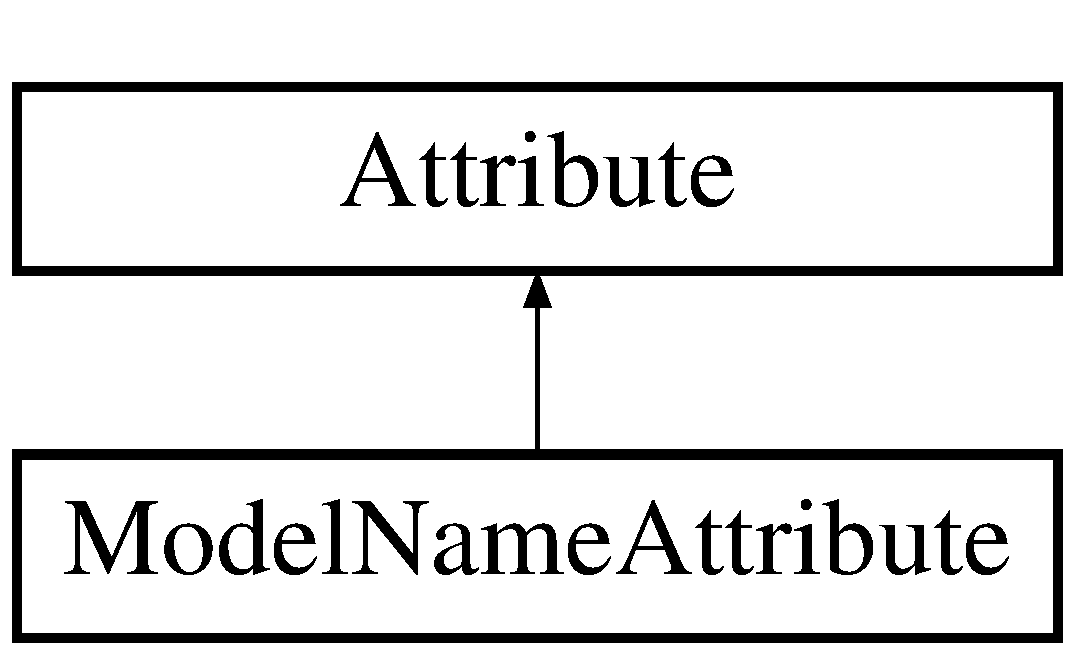
\includegraphics[height=2.000000cm]{classApi3Layers_1_1Areas_1_1HelpPage_1_1ModelDescriptions_1_1ModelNameAttribute}
\end{center}
\end{figure}
\subsection*{Métodos Públicos}
\begin{DoxyCompactItemize}
\item 
\hyperlink{classApi3Layers_1_1Areas_1_1HelpPage_1_1ModelDescriptions_1_1ModelNameAttribute_a0e5f4a1f1b6fb75cb7804f6905744f39}{Model\+Name\+Attribute} (string name)
\end{DoxyCompactItemize}
\subsection*{Propriedades}
\begin{DoxyCompactItemize}
\item 
string \hyperlink{classApi3Layers_1_1Areas_1_1HelpPage_1_1ModelDescriptions_1_1ModelNameAttribute_a7ee9065718e6628dc7791b756fa6c0f9}{Name}\hspace{0.3cm}{\ttfamily  \mbox{[}get, private set\mbox{]}}
\end{DoxyCompactItemize}


\subsection{Descrição Detalhada}
Use this attribute to change the name of the \hyperlink{classApi3Layers_1_1Areas_1_1HelpPage_1_1ModelDescriptions_1_1ModelDescription}{Model\+Description} generated for a type. 



\subsection{Construtores \& Destrutores}
\mbox{\Hypertarget{classApi3Layers_1_1Areas_1_1HelpPage_1_1ModelDescriptions_1_1ModelNameAttribute_a0e5f4a1f1b6fb75cb7804f6905744f39}\label{classApi3Layers_1_1Areas_1_1HelpPage_1_1ModelDescriptions_1_1ModelNameAttribute_a0e5f4a1f1b6fb75cb7804f6905744f39}} 
\index{Api3\+Layers\+::\+Areas\+::\+Help\+Page\+::\+Model\+Descriptions\+::\+Model\+Name\+Attribute@{Api3\+Layers\+::\+Areas\+::\+Help\+Page\+::\+Model\+Descriptions\+::\+Model\+Name\+Attribute}!Model\+Name\+Attribute@{Model\+Name\+Attribute}}
\index{Model\+Name\+Attribute@{Model\+Name\+Attribute}!Api3\+Layers\+::\+Areas\+::\+Help\+Page\+::\+Model\+Descriptions\+::\+Model\+Name\+Attribute@{Api3\+Layers\+::\+Areas\+::\+Help\+Page\+::\+Model\+Descriptions\+::\+Model\+Name\+Attribute}}
\subsubsection{\texorpdfstring{Model\+Name\+Attribute()}{ModelNameAttribute()}}
{\footnotesize\ttfamily \hyperlink{classApi3Layers_1_1Areas_1_1HelpPage_1_1ModelDescriptions_1_1ModelNameAttribute}{Model\+Name\+Attribute} (\begin{DoxyParamCaption}\item[{string}]{name }\end{DoxyParamCaption})}



\subsection{Propriedades}
\mbox{\Hypertarget{classApi3Layers_1_1Areas_1_1HelpPage_1_1ModelDescriptions_1_1ModelNameAttribute_a7ee9065718e6628dc7791b756fa6c0f9}\label{classApi3Layers_1_1Areas_1_1HelpPage_1_1ModelDescriptions_1_1ModelNameAttribute_a7ee9065718e6628dc7791b756fa6c0f9}} 
\index{Api3\+Layers\+::\+Areas\+::\+Help\+Page\+::\+Model\+Descriptions\+::\+Model\+Name\+Attribute@{Api3\+Layers\+::\+Areas\+::\+Help\+Page\+::\+Model\+Descriptions\+::\+Model\+Name\+Attribute}!Name@{Name}}
\index{Name@{Name}!Api3\+Layers\+::\+Areas\+::\+Help\+Page\+::\+Model\+Descriptions\+::\+Model\+Name\+Attribute@{Api3\+Layers\+::\+Areas\+::\+Help\+Page\+::\+Model\+Descriptions\+::\+Model\+Name\+Attribute}}
\subsubsection{\texorpdfstring{Name}{Name}}
{\footnotesize\ttfamily string Name\hspace{0.3cm}{\ttfamily [get]}, {\ttfamily [private set]}}



A documentação para esta classe foi gerada a partir do seguinte arquivo\+:\begin{DoxyCompactItemize}
\item 
Api3\+Layers/\+Areas/\+Help\+Page/\+Model\+Descriptions/\hyperlink{ModelNameAttribute_8cs}{Model\+Name\+Attribute.\+cs}\end{DoxyCompactItemize}

\hypertarget{classApi3Layers_1_1Areas_1_1HelpPage_1_1ModelDescriptions_1_1ModelNameHelper}{}\section{Model\+Name\+Helper}
\label{classApi3Layers_1_1Areas_1_1HelpPage_1_1ModelDescriptions_1_1ModelNameHelper}\index{Model\+Name\+Helper@{Model\+Name\+Helper}}
\subsection*{Métodos Públicos Estáticos}
\begin{DoxyCompactItemize}
\item 
static string \hyperlink{classApi3Layers_1_1Areas_1_1HelpPage_1_1ModelDescriptions_1_1ModelNameHelper_a94996770939db3fd96b3421ea1907cdb}{Get\+Model\+Name} (Type type)
\end{DoxyCompactItemize}


\subsection{Métodos}
\mbox{\Hypertarget{classApi3Layers_1_1Areas_1_1HelpPage_1_1ModelDescriptions_1_1ModelNameHelper_a94996770939db3fd96b3421ea1907cdb}\label{classApi3Layers_1_1Areas_1_1HelpPage_1_1ModelDescriptions_1_1ModelNameHelper_a94996770939db3fd96b3421ea1907cdb}} 
\index{Api3\+Layers\+::\+Areas\+::\+Help\+Page\+::\+Model\+Descriptions\+::\+Model\+Name\+Helper@{Api3\+Layers\+::\+Areas\+::\+Help\+Page\+::\+Model\+Descriptions\+::\+Model\+Name\+Helper}!Get\+Model\+Name@{Get\+Model\+Name}}
\index{Get\+Model\+Name@{Get\+Model\+Name}!Api3\+Layers\+::\+Areas\+::\+Help\+Page\+::\+Model\+Descriptions\+::\+Model\+Name\+Helper@{Api3\+Layers\+::\+Areas\+::\+Help\+Page\+::\+Model\+Descriptions\+::\+Model\+Name\+Helper}}
\subsubsection{\texorpdfstring{Get\+Model\+Name()}{GetModelName()}}
{\footnotesize\ttfamily static string Get\+Model\+Name (\begin{DoxyParamCaption}\item[{Type}]{type }\end{DoxyParamCaption})\hspace{0.3cm}{\ttfamily [static]}}



A documentação para esta classe foi gerada a partir do seguinte arquivo\+:\begin{DoxyCompactItemize}
\item 
C\+:/\+Users/\+Bruno/\+Desktop/\+Api3\+Layers/\+Api3\+Layers/\+Areas/\+Help\+Page/\+Model\+Descriptions/\hyperlink{ModelNameHelper_8cs}{Model\+Name\+Helper.\+cs}\end{DoxyCompactItemize}

\hypertarget{classApi3Layers_1_1Areas_1_1HelpPage_1_1ModelDescriptions_1_1ParameterAnnotation}{}\section{Parameter\+Annotation}
\label{classApi3Layers_1_1Areas_1_1HelpPage_1_1ModelDescriptions_1_1ParameterAnnotation}\index{Parameter\+Annotation@{Parameter\+Annotation}}
\subsection*{Propriedades}
\begin{DoxyCompactItemize}
\item 
Attribute \hyperlink{classApi3Layers_1_1Areas_1_1HelpPage_1_1ModelDescriptions_1_1ParameterAnnotation_a392dedd976c4dc366de9e5b213c4e716}{Annotation\+Attribute}\hspace{0.3cm}{\ttfamily  \mbox{[}get, set\mbox{]}}
\item 
string \hyperlink{classApi3Layers_1_1Areas_1_1HelpPage_1_1ModelDescriptions_1_1ParameterAnnotation_a239e2715951fcab2d9b263ef6acfa899}{Documentation}\hspace{0.3cm}{\ttfamily  \mbox{[}get, set\mbox{]}}
\end{DoxyCompactItemize}


\subsection{Propriedades}
\mbox{\Hypertarget{classApi3Layers_1_1Areas_1_1HelpPage_1_1ModelDescriptions_1_1ParameterAnnotation_a392dedd976c4dc366de9e5b213c4e716}\label{classApi3Layers_1_1Areas_1_1HelpPage_1_1ModelDescriptions_1_1ParameterAnnotation_a392dedd976c4dc366de9e5b213c4e716}} 
\index{Api3\+Layers\+::\+Areas\+::\+Help\+Page\+::\+Model\+Descriptions\+::\+Parameter\+Annotation@{Api3\+Layers\+::\+Areas\+::\+Help\+Page\+::\+Model\+Descriptions\+::\+Parameter\+Annotation}!Annotation\+Attribute@{Annotation\+Attribute}}
\index{Annotation\+Attribute@{Annotation\+Attribute}!Api3\+Layers\+::\+Areas\+::\+Help\+Page\+::\+Model\+Descriptions\+::\+Parameter\+Annotation@{Api3\+Layers\+::\+Areas\+::\+Help\+Page\+::\+Model\+Descriptions\+::\+Parameter\+Annotation}}
\subsubsection{\texorpdfstring{Annotation\+Attribute}{AnnotationAttribute}}
{\footnotesize\ttfamily Attribute Annotation\+Attribute\hspace{0.3cm}{\ttfamily [get]}, {\ttfamily [set]}}

\mbox{\Hypertarget{classApi3Layers_1_1Areas_1_1HelpPage_1_1ModelDescriptions_1_1ParameterAnnotation_a239e2715951fcab2d9b263ef6acfa899}\label{classApi3Layers_1_1Areas_1_1HelpPage_1_1ModelDescriptions_1_1ParameterAnnotation_a239e2715951fcab2d9b263ef6acfa899}} 
\index{Api3\+Layers\+::\+Areas\+::\+Help\+Page\+::\+Model\+Descriptions\+::\+Parameter\+Annotation@{Api3\+Layers\+::\+Areas\+::\+Help\+Page\+::\+Model\+Descriptions\+::\+Parameter\+Annotation}!Documentation@{Documentation}}
\index{Documentation@{Documentation}!Api3\+Layers\+::\+Areas\+::\+Help\+Page\+::\+Model\+Descriptions\+::\+Parameter\+Annotation@{Api3\+Layers\+::\+Areas\+::\+Help\+Page\+::\+Model\+Descriptions\+::\+Parameter\+Annotation}}
\subsubsection{\texorpdfstring{Documentation}{Documentation}}
{\footnotesize\ttfamily string Documentation\hspace{0.3cm}{\ttfamily [get]}, {\ttfamily [set]}}



A documentação para esta classe foi gerada a partir do seguinte arquivo\+:\begin{DoxyCompactItemize}
\item 
C\+:/\+Users/\+Bruno/\+Desktop/\+Api3\+Layers/\+Api3\+Layers/\+Areas/\+Help\+Page/\+Model\+Descriptions/\hyperlink{ParameterAnnotation_8cs}{Parameter\+Annotation.\+cs}\end{DoxyCompactItemize}

\hypertarget{classApi3Layers_1_1Areas_1_1HelpPage_1_1ModelDescriptions_1_1ParameterDescription}{}\section{Parameter\+Description}
\label{classApi3Layers_1_1Areas_1_1HelpPage_1_1ModelDescriptions_1_1ParameterDescription}\index{Parameter\+Description@{Parameter\+Description}}
\subsection*{Métodos Públicos}
\begin{DoxyCompactItemize}
\item 
\hyperlink{classApi3Layers_1_1Areas_1_1HelpPage_1_1ModelDescriptions_1_1ParameterDescription_aefb4a1da3e61b3368645c8f2fd71a50f}{Parameter\+Description} ()
\end{DoxyCompactItemize}
\subsection*{Propriedades}
\begin{DoxyCompactItemize}
\item 
Collection$<$ \hyperlink{classApi3Layers_1_1Areas_1_1HelpPage_1_1ModelDescriptions_1_1ParameterAnnotation}{Parameter\+Annotation} $>$ \hyperlink{classApi3Layers_1_1Areas_1_1HelpPage_1_1ModelDescriptions_1_1ParameterDescription_ae2e50db897fe523b76e76972dfdce1ce}{Annotations}\hspace{0.3cm}{\ttfamily  \mbox{[}get, private set\mbox{]}}
\item 
string \hyperlink{classApi3Layers_1_1Areas_1_1HelpPage_1_1ModelDescriptions_1_1ParameterDescription_a239e2715951fcab2d9b263ef6acfa899}{Documentation}\hspace{0.3cm}{\ttfamily  \mbox{[}get, set\mbox{]}}
\item 
string \hyperlink{classApi3Layers_1_1Areas_1_1HelpPage_1_1ModelDescriptions_1_1ParameterDescription_a7ee9065718e6628dc7791b756fa6c0f9}{Name}\hspace{0.3cm}{\ttfamily  \mbox{[}get, set\mbox{]}}
\item 
\hyperlink{classApi3Layers_1_1Areas_1_1HelpPage_1_1ModelDescriptions_1_1ModelDescription}{Model\+Description} \hyperlink{classApi3Layers_1_1Areas_1_1HelpPage_1_1ModelDescriptions_1_1ParameterDescription_a53f61645aec0f2428fcac91ce7db2995}{Type\+Description}\hspace{0.3cm}{\ttfamily  \mbox{[}get, set\mbox{]}}
\end{DoxyCompactItemize}


\subsection{Construtores \& Destrutores}
\mbox{\Hypertarget{classApi3Layers_1_1Areas_1_1HelpPage_1_1ModelDescriptions_1_1ParameterDescription_aefb4a1da3e61b3368645c8f2fd71a50f}\label{classApi3Layers_1_1Areas_1_1HelpPage_1_1ModelDescriptions_1_1ParameterDescription_aefb4a1da3e61b3368645c8f2fd71a50f}} 
\index{Api3\+Layers\+::\+Areas\+::\+Help\+Page\+::\+Model\+Descriptions\+::\+Parameter\+Description@{Api3\+Layers\+::\+Areas\+::\+Help\+Page\+::\+Model\+Descriptions\+::\+Parameter\+Description}!Parameter\+Description@{Parameter\+Description}}
\index{Parameter\+Description@{Parameter\+Description}!Api3\+Layers\+::\+Areas\+::\+Help\+Page\+::\+Model\+Descriptions\+::\+Parameter\+Description@{Api3\+Layers\+::\+Areas\+::\+Help\+Page\+::\+Model\+Descriptions\+::\+Parameter\+Description}}
\subsubsection{\texorpdfstring{Parameter\+Description()}{ParameterDescription()}}
{\footnotesize\ttfamily \hyperlink{classApi3Layers_1_1Areas_1_1HelpPage_1_1ModelDescriptions_1_1ParameterDescription}{Parameter\+Description} (\begin{DoxyParamCaption}{ }\end{DoxyParamCaption})}



\subsection{Propriedades}
\mbox{\Hypertarget{classApi3Layers_1_1Areas_1_1HelpPage_1_1ModelDescriptions_1_1ParameterDescription_ae2e50db897fe523b76e76972dfdce1ce}\label{classApi3Layers_1_1Areas_1_1HelpPage_1_1ModelDescriptions_1_1ParameterDescription_ae2e50db897fe523b76e76972dfdce1ce}} 
\index{Api3\+Layers\+::\+Areas\+::\+Help\+Page\+::\+Model\+Descriptions\+::\+Parameter\+Description@{Api3\+Layers\+::\+Areas\+::\+Help\+Page\+::\+Model\+Descriptions\+::\+Parameter\+Description}!Annotations@{Annotations}}
\index{Annotations@{Annotations}!Api3\+Layers\+::\+Areas\+::\+Help\+Page\+::\+Model\+Descriptions\+::\+Parameter\+Description@{Api3\+Layers\+::\+Areas\+::\+Help\+Page\+::\+Model\+Descriptions\+::\+Parameter\+Description}}
\subsubsection{\texorpdfstring{Annotations}{Annotations}}
{\footnotesize\ttfamily Collection$<$\hyperlink{classApi3Layers_1_1Areas_1_1HelpPage_1_1ModelDescriptions_1_1ParameterAnnotation}{Parameter\+Annotation}$>$ Annotations\hspace{0.3cm}{\ttfamily [get]}, {\ttfamily [private set]}}

\mbox{\Hypertarget{classApi3Layers_1_1Areas_1_1HelpPage_1_1ModelDescriptions_1_1ParameterDescription_a239e2715951fcab2d9b263ef6acfa899}\label{classApi3Layers_1_1Areas_1_1HelpPage_1_1ModelDescriptions_1_1ParameterDescription_a239e2715951fcab2d9b263ef6acfa899}} 
\index{Api3\+Layers\+::\+Areas\+::\+Help\+Page\+::\+Model\+Descriptions\+::\+Parameter\+Description@{Api3\+Layers\+::\+Areas\+::\+Help\+Page\+::\+Model\+Descriptions\+::\+Parameter\+Description}!Documentation@{Documentation}}
\index{Documentation@{Documentation}!Api3\+Layers\+::\+Areas\+::\+Help\+Page\+::\+Model\+Descriptions\+::\+Parameter\+Description@{Api3\+Layers\+::\+Areas\+::\+Help\+Page\+::\+Model\+Descriptions\+::\+Parameter\+Description}}
\subsubsection{\texorpdfstring{Documentation}{Documentation}}
{\footnotesize\ttfamily string Documentation\hspace{0.3cm}{\ttfamily [get]}, {\ttfamily [set]}}

\mbox{\Hypertarget{classApi3Layers_1_1Areas_1_1HelpPage_1_1ModelDescriptions_1_1ParameterDescription_a7ee9065718e6628dc7791b756fa6c0f9}\label{classApi3Layers_1_1Areas_1_1HelpPage_1_1ModelDescriptions_1_1ParameterDescription_a7ee9065718e6628dc7791b756fa6c0f9}} 
\index{Api3\+Layers\+::\+Areas\+::\+Help\+Page\+::\+Model\+Descriptions\+::\+Parameter\+Description@{Api3\+Layers\+::\+Areas\+::\+Help\+Page\+::\+Model\+Descriptions\+::\+Parameter\+Description}!Name@{Name}}
\index{Name@{Name}!Api3\+Layers\+::\+Areas\+::\+Help\+Page\+::\+Model\+Descriptions\+::\+Parameter\+Description@{Api3\+Layers\+::\+Areas\+::\+Help\+Page\+::\+Model\+Descriptions\+::\+Parameter\+Description}}
\subsubsection{\texorpdfstring{Name}{Name}}
{\footnotesize\ttfamily string Name\hspace{0.3cm}{\ttfamily [get]}, {\ttfamily [set]}}

\mbox{\Hypertarget{classApi3Layers_1_1Areas_1_1HelpPage_1_1ModelDescriptions_1_1ParameterDescription_a53f61645aec0f2428fcac91ce7db2995}\label{classApi3Layers_1_1Areas_1_1HelpPage_1_1ModelDescriptions_1_1ParameterDescription_a53f61645aec0f2428fcac91ce7db2995}} 
\index{Api3\+Layers\+::\+Areas\+::\+Help\+Page\+::\+Model\+Descriptions\+::\+Parameter\+Description@{Api3\+Layers\+::\+Areas\+::\+Help\+Page\+::\+Model\+Descriptions\+::\+Parameter\+Description}!Type\+Description@{Type\+Description}}
\index{Type\+Description@{Type\+Description}!Api3\+Layers\+::\+Areas\+::\+Help\+Page\+::\+Model\+Descriptions\+::\+Parameter\+Description@{Api3\+Layers\+::\+Areas\+::\+Help\+Page\+::\+Model\+Descriptions\+::\+Parameter\+Description}}
\subsubsection{\texorpdfstring{Type\+Description}{TypeDescription}}
{\footnotesize\ttfamily \hyperlink{classApi3Layers_1_1Areas_1_1HelpPage_1_1ModelDescriptions_1_1ModelDescription}{Model\+Description} Type\+Description\hspace{0.3cm}{\ttfamily [get]}, {\ttfamily [set]}}



A documentação para esta classe foi gerada a partir do seguinte arquivo\+:\begin{DoxyCompactItemize}
\item 
Api3\+Layers/\+Areas/\+Help\+Page/\+Model\+Descriptions/\hyperlink{ParameterDescription_8cs}{Parameter\+Description.\+cs}\end{DoxyCompactItemize}

\hypertarget{classApi3Layers_1_1Areas_1_1HelpPage_1_1ModelDescriptions_1_1SimpleTypeModelDescription}{}\section{Simple\+Type\+Model\+Description}
\label{classApi3Layers_1_1Areas_1_1HelpPage_1_1ModelDescriptions_1_1SimpleTypeModelDescription}\index{Simple\+Type\+Model\+Description@{Simple\+Type\+Model\+Description}}
Diagrama de Hierarquia para Simple\+Type\+Model\+Description\+:\begin{figure}[H]
\begin{center}
\leavevmode
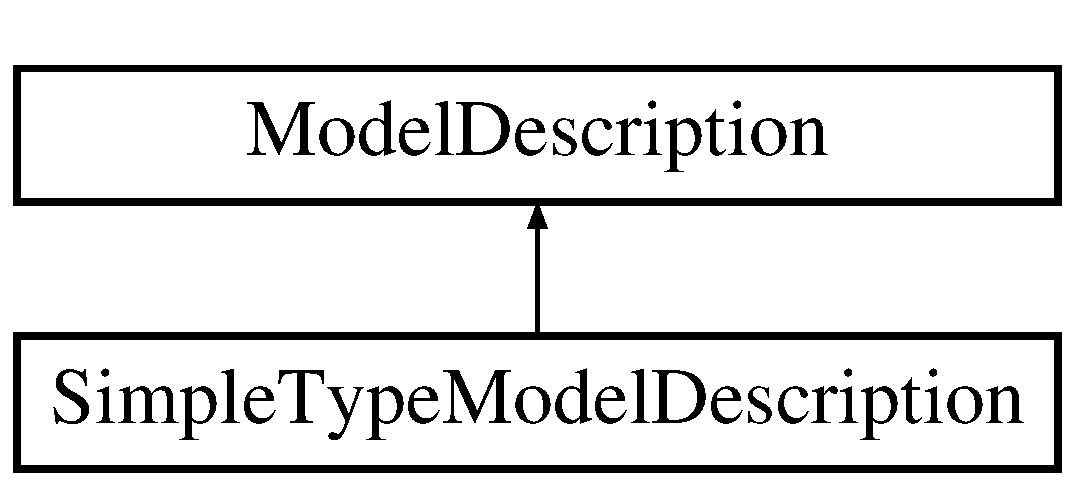
\includegraphics[height=2.000000cm]{classApi3Layers_1_1Areas_1_1HelpPage_1_1ModelDescriptions_1_1SimpleTypeModelDescription}
\end{center}
\end{figure}
\subsection*{Outros membros herdados}


A documentação para esta classe foi gerada a partir do seguinte arquivo\+:\begin{DoxyCompactItemize}
\item 
Api3\+Layers/\+Areas/\+Help\+Page/\+Model\+Descriptions/\hyperlink{SimpleTypeModelDescription_8cs}{Simple\+Type\+Model\+Description.\+cs}\end{DoxyCompactItemize}

\hypertarget{classApi3Layers_1_1Areas_1_1HelpPage_1_1Models_1_1HelpPageApiModel}{}\section{Help\+Page\+Api\+Model}
\label{classApi3Layers_1_1Areas_1_1HelpPage_1_1Models_1_1HelpPageApiModel}\index{Help\+Page\+Api\+Model@{Help\+Page\+Api\+Model}}


The model that represents an A\+PI displayed on the help page.  


\subsection*{Métodos Públicos}
\begin{DoxyCompactItemize}
\item 
\hyperlink{classApi3Layers_1_1Areas_1_1HelpPage_1_1Models_1_1HelpPageApiModel_a0743b6d8422d1b857b2bfccee21d846c}{Help\+Page\+Api\+Model} ()
\begin{DoxyCompactList}\small\item\em Initializes a new instance of the \hyperlink{classApi3Layers_1_1Areas_1_1HelpPage_1_1Models_1_1HelpPageApiModel}{Help\+Page\+Api\+Model} class. \end{DoxyCompactList}\end{DoxyCompactItemize}
\subsection*{Propriedades}
\begin{DoxyCompactItemize}
\item 
Api\+Description \hyperlink{classApi3Layers_1_1Areas_1_1HelpPage_1_1Models_1_1HelpPageApiModel_ad1a6fd4ef907b1fdba9bba7d46fe5992}{Api\+Description}\hspace{0.3cm}{\ttfamily  \mbox{[}get, set\mbox{]}}
\begin{DoxyCompactList}\small\item\em Gets or sets the \hyperlink{classApi3Layers_1_1Areas_1_1HelpPage_1_1Models_1_1HelpPageApiModel_ad1a6fd4ef907b1fdba9bba7d46fe5992}{Api\+Description} that describes the A\+PI. \end{DoxyCompactList}\item 
Collection$<$ string $>$ \hyperlink{classApi3Layers_1_1Areas_1_1HelpPage_1_1Models_1_1HelpPageApiModel_ad066016c7ca05c83bd336000adaa9a34}{Error\+Messages}\hspace{0.3cm}{\ttfamily  \mbox{[}get, private set\mbox{]}}
\begin{DoxyCompactList}\small\item\em Gets the error messages associated with this model. \end{DoxyCompactList}\item 
I\+List$<$ \hyperlink{classApi3Layers_1_1Areas_1_1HelpPage_1_1ModelDescriptions_1_1ParameterDescription}{Parameter\+Description} $>$ \hyperlink{classApi3Layers_1_1Areas_1_1HelpPage_1_1Models_1_1HelpPageApiModel_afa8a93fe41667b75d8e8bb82464b0ce9}{Request\+Body\+Parameters}\hspace{0.3cm}{\ttfamily  \mbox{[}get\mbox{]}}
\begin{DoxyCompactList}\small\item\em Gets the request body parameter descriptions. \end{DoxyCompactList}\item 
string \hyperlink{classApi3Layers_1_1Areas_1_1HelpPage_1_1Models_1_1HelpPageApiModel_a444fbff8827e51d426af83b50f6f09db}{Request\+Documentation}\hspace{0.3cm}{\ttfamily  \mbox{[}get, set\mbox{]}}
\begin{DoxyCompactList}\small\item\em Gets or sets the documentation for the request. \end{DoxyCompactList}\item 
\hyperlink{classApi3Layers_1_1Areas_1_1HelpPage_1_1ModelDescriptions_1_1ModelDescription}{Model\+Description} \hyperlink{classApi3Layers_1_1Areas_1_1HelpPage_1_1Models_1_1HelpPageApiModel_a014cdaab9901575d2ad288db94d49d49}{Request\+Model\+Description}\hspace{0.3cm}{\ttfamily  \mbox{[}get, set\mbox{]}}
\begin{DoxyCompactList}\small\item\em Gets or sets the Model\+Description that describes the request body. \end{DoxyCompactList}\item 
\hyperlink{classApi3Layers_1_1Areas_1_1HelpPage_1_1ModelDescriptions_1_1ModelDescription}{Model\+Description} \hyperlink{classApi3Layers_1_1Areas_1_1HelpPage_1_1Models_1_1HelpPageApiModel_aac9145223442cf500f314efff3ba18a6}{Resource\+Description}\hspace{0.3cm}{\ttfamily  \mbox{[}get, set\mbox{]}}
\begin{DoxyCompactList}\small\item\em Gets or sets the Model\+Description that describes the resource. \end{DoxyCompactList}\item 
I\+List$<$ \hyperlink{classApi3Layers_1_1Areas_1_1HelpPage_1_1ModelDescriptions_1_1ParameterDescription}{Parameter\+Description} $>$ \hyperlink{classApi3Layers_1_1Areas_1_1HelpPage_1_1Models_1_1HelpPageApiModel_aa66bf0e93d9891ddd4d05c986f886475}{Resource\+Properties}\hspace{0.3cm}{\ttfamily  \mbox{[}get\mbox{]}}
\begin{DoxyCompactList}\small\item\em Gets the resource property descriptions. \end{DoxyCompactList}\item 
I\+Dictionary$<$ Media\+Type\+Header\+Value, object $>$ \hyperlink{classApi3Layers_1_1Areas_1_1HelpPage_1_1Models_1_1HelpPageApiModel_af027805b3af135bd56af841959479958}{Sample\+Requests}\hspace{0.3cm}{\ttfamily  \mbox{[}get, private set\mbox{]}}
\begin{DoxyCompactList}\small\item\em Gets the sample requests associated with the A\+PI. \end{DoxyCompactList}\item 
I\+Dictionary$<$ Media\+Type\+Header\+Value, object $>$ \hyperlink{classApi3Layers_1_1Areas_1_1HelpPage_1_1Models_1_1HelpPageApiModel_a4d0e8d9e76b2cc139ae6c1c0ba205f92}{Sample\+Responses}\hspace{0.3cm}{\ttfamily  \mbox{[}get, private set\mbox{]}}
\begin{DoxyCompactList}\small\item\em Gets the sample responses associated with the A\+PI. \end{DoxyCompactList}\item 
Collection$<$ \hyperlink{classApi3Layers_1_1Areas_1_1HelpPage_1_1ModelDescriptions_1_1ParameterDescription}{Parameter\+Description} $>$ \hyperlink{classApi3Layers_1_1Areas_1_1HelpPage_1_1Models_1_1HelpPageApiModel_a2f4ee03fa855608076ab48dc71fb61f5}{Uri\+Parameters}\hspace{0.3cm}{\ttfamily  \mbox{[}get, private set\mbox{]}}
\begin{DoxyCompactList}\small\item\em Gets or sets the Parameter\+Description collection that describes the U\+RI parameters for the A\+PI. \end{DoxyCompactList}\end{DoxyCompactItemize}
\subsection*{Métodos Privados Estáticos}
\begin{DoxyCompactItemize}
\item 
static I\+List$<$ \hyperlink{classApi3Layers_1_1Areas_1_1HelpPage_1_1ModelDescriptions_1_1ParameterDescription}{Parameter\+Description} $>$ \hyperlink{classApi3Layers_1_1Areas_1_1HelpPage_1_1Models_1_1HelpPageApiModel_a46f28b264ed67e8b868762020f049126}{Get\+Parameter\+Descriptions} (\hyperlink{classApi3Layers_1_1Areas_1_1HelpPage_1_1ModelDescriptions_1_1ModelDescription}{Model\+Description} model\+Description)
\end{DoxyCompactItemize}


\subsection{Descrição Detalhada}
The model that represents an A\+PI displayed on the help page. 



\subsection{Construtores \& Destrutores}
\mbox{\Hypertarget{classApi3Layers_1_1Areas_1_1HelpPage_1_1Models_1_1HelpPageApiModel_a0743b6d8422d1b857b2bfccee21d846c}\label{classApi3Layers_1_1Areas_1_1HelpPage_1_1Models_1_1HelpPageApiModel_a0743b6d8422d1b857b2bfccee21d846c}} 
\index{Api3\+Layers\+::\+Areas\+::\+Help\+Page\+::\+Models\+::\+Help\+Page\+Api\+Model@{Api3\+Layers\+::\+Areas\+::\+Help\+Page\+::\+Models\+::\+Help\+Page\+Api\+Model}!Help\+Page\+Api\+Model@{Help\+Page\+Api\+Model}}
\index{Help\+Page\+Api\+Model@{Help\+Page\+Api\+Model}!Api3\+Layers\+::\+Areas\+::\+Help\+Page\+::\+Models\+::\+Help\+Page\+Api\+Model@{Api3\+Layers\+::\+Areas\+::\+Help\+Page\+::\+Models\+::\+Help\+Page\+Api\+Model}}
\subsubsection{\texorpdfstring{Help\+Page\+Api\+Model()}{HelpPageApiModel()}}
{\footnotesize\ttfamily \hyperlink{classApi3Layers_1_1Areas_1_1HelpPage_1_1Models_1_1HelpPageApiModel}{Help\+Page\+Api\+Model} (\begin{DoxyParamCaption}{ }\end{DoxyParamCaption})}



Initializes a new instance of the \hyperlink{classApi3Layers_1_1Areas_1_1HelpPage_1_1Models_1_1HelpPageApiModel}{Help\+Page\+Api\+Model} class. 



\subsection{Métodos}
\mbox{\Hypertarget{classApi3Layers_1_1Areas_1_1HelpPage_1_1Models_1_1HelpPageApiModel_a46f28b264ed67e8b868762020f049126}\label{classApi3Layers_1_1Areas_1_1HelpPage_1_1Models_1_1HelpPageApiModel_a46f28b264ed67e8b868762020f049126}} 
\index{Api3\+Layers\+::\+Areas\+::\+Help\+Page\+::\+Models\+::\+Help\+Page\+Api\+Model@{Api3\+Layers\+::\+Areas\+::\+Help\+Page\+::\+Models\+::\+Help\+Page\+Api\+Model}!Get\+Parameter\+Descriptions@{Get\+Parameter\+Descriptions}}
\index{Get\+Parameter\+Descriptions@{Get\+Parameter\+Descriptions}!Api3\+Layers\+::\+Areas\+::\+Help\+Page\+::\+Models\+::\+Help\+Page\+Api\+Model@{Api3\+Layers\+::\+Areas\+::\+Help\+Page\+::\+Models\+::\+Help\+Page\+Api\+Model}}
\subsubsection{\texorpdfstring{Get\+Parameter\+Descriptions()}{GetParameterDescriptions()}}
{\footnotesize\ttfamily static I\+List$<$\hyperlink{classApi3Layers_1_1Areas_1_1HelpPage_1_1ModelDescriptions_1_1ParameterDescription}{Parameter\+Description}$>$ Get\+Parameter\+Descriptions (\begin{DoxyParamCaption}\item[{\hyperlink{classApi3Layers_1_1Areas_1_1HelpPage_1_1ModelDescriptions_1_1ModelDescription}{Model\+Description}}]{model\+Description }\end{DoxyParamCaption})\hspace{0.3cm}{\ttfamily [static]}, {\ttfamily [private]}}



\subsection{Propriedades}
\mbox{\Hypertarget{classApi3Layers_1_1Areas_1_1HelpPage_1_1Models_1_1HelpPageApiModel_ad1a6fd4ef907b1fdba9bba7d46fe5992}\label{classApi3Layers_1_1Areas_1_1HelpPage_1_1Models_1_1HelpPageApiModel_ad1a6fd4ef907b1fdba9bba7d46fe5992}} 
\index{Api3\+Layers\+::\+Areas\+::\+Help\+Page\+::\+Models\+::\+Help\+Page\+Api\+Model@{Api3\+Layers\+::\+Areas\+::\+Help\+Page\+::\+Models\+::\+Help\+Page\+Api\+Model}!Api\+Description@{Api\+Description}}
\index{Api\+Description@{Api\+Description}!Api3\+Layers\+::\+Areas\+::\+Help\+Page\+::\+Models\+::\+Help\+Page\+Api\+Model@{Api3\+Layers\+::\+Areas\+::\+Help\+Page\+::\+Models\+::\+Help\+Page\+Api\+Model}}
\subsubsection{\texorpdfstring{Api\+Description}{ApiDescription}}
{\footnotesize\ttfamily Api\+Description Api\+Description\hspace{0.3cm}{\ttfamily [get]}, {\ttfamily [set]}}



Gets or sets the \hyperlink{classApi3Layers_1_1Areas_1_1HelpPage_1_1Models_1_1HelpPageApiModel_ad1a6fd4ef907b1fdba9bba7d46fe5992}{Api\+Description} that describes the A\+PI. 

\mbox{\Hypertarget{classApi3Layers_1_1Areas_1_1HelpPage_1_1Models_1_1HelpPageApiModel_ad066016c7ca05c83bd336000adaa9a34}\label{classApi3Layers_1_1Areas_1_1HelpPage_1_1Models_1_1HelpPageApiModel_ad066016c7ca05c83bd336000adaa9a34}} 
\index{Api3\+Layers\+::\+Areas\+::\+Help\+Page\+::\+Models\+::\+Help\+Page\+Api\+Model@{Api3\+Layers\+::\+Areas\+::\+Help\+Page\+::\+Models\+::\+Help\+Page\+Api\+Model}!Error\+Messages@{Error\+Messages}}
\index{Error\+Messages@{Error\+Messages}!Api3\+Layers\+::\+Areas\+::\+Help\+Page\+::\+Models\+::\+Help\+Page\+Api\+Model@{Api3\+Layers\+::\+Areas\+::\+Help\+Page\+::\+Models\+::\+Help\+Page\+Api\+Model}}
\subsubsection{\texorpdfstring{Error\+Messages}{ErrorMessages}}
{\footnotesize\ttfamily Collection$<$string$>$ Error\+Messages\hspace{0.3cm}{\ttfamily [get]}, {\ttfamily [private set]}}



Gets the error messages associated with this model. 

\mbox{\Hypertarget{classApi3Layers_1_1Areas_1_1HelpPage_1_1Models_1_1HelpPageApiModel_afa8a93fe41667b75d8e8bb82464b0ce9}\label{classApi3Layers_1_1Areas_1_1HelpPage_1_1Models_1_1HelpPageApiModel_afa8a93fe41667b75d8e8bb82464b0ce9}} 
\index{Api3\+Layers\+::\+Areas\+::\+Help\+Page\+::\+Models\+::\+Help\+Page\+Api\+Model@{Api3\+Layers\+::\+Areas\+::\+Help\+Page\+::\+Models\+::\+Help\+Page\+Api\+Model}!Request\+Body\+Parameters@{Request\+Body\+Parameters}}
\index{Request\+Body\+Parameters@{Request\+Body\+Parameters}!Api3\+Layers\+::\+Areas\+::\+Help\+Page\+::\+Models\+::\+Help\+Page\+Api\+Model@{Api3\+Layers\+::\+Areas\+::\+Help\+Page\+::\+Models\+::\+Help\+Page\+Api\+Model}}
\subsubsection{\texorpdfstring{Request\+Body\+Parameters}{RequestBodyParameters}}
{\footnotesize\ttfamily I\+List$<$\hyperlink{classApi3Layers_1_1Areas_1_1HelpPage_1_1ModelDescriptions_1_1ParameterDescription}{Parameter\+Description}$>$ Request\+Body\+Parameters\hspace{0.3cm}{\ttfamily [get]}}



Gets the request body parameter descriptions. 

\mbox{\Hypertarget{classApi3Layers_1_1Areas_1_1HelpPage_1_1Models_1_1HelpPageApiModel_a444fbff8827e51d426af83b50f6f09db}\label{classApi3Layers_1_1Areas_1_1HelpPage_1_1Models_1_1HelpPageApiModel_a444fbff8827e51d426af83b50f6f09db}} 
\index{Api3\+Layers\+::\+Areas\+::\+Help\+Page\+::\+Models\+::\+Help\+Page\+Api\+Model@{Api3\+Layers\+::\+Areas\+::\+Help\+Page\+::\+Models\+::\+Help\+Page\+Api\+Model}!Request\+Documentation@{Request\+Documentation}}
\index{Request\+Documentation@{Request\+Documentation}!Api3\+Layers\+::\+Areas\+::\+Help\+Page\+::\+Models\+::\+Help\+Page\+Api\+Model@{Api3\+Layers\+::\+Areas\+::\+Help\+Page\+::\+Models\+::\+Help\+Page\+Api\+Model}}
\subsubsection{\texorpdfstring{Request\+Documentation}{RequestDocumentation}}
{\footnotesize\ttfamily string Request\+Documentation\hspace{0.3cm}{\ttfamily [get]}, {\ttfamily [set]}}



Gets or sets the documentation for the request. 

\mbox{\Hypertarget{classApi3Layers_1_1Areas_1_1HelpPage_1_1Models_1_1HelpPageApiModel_a014cdaab9901575d2ad288db94d49d49}\label{classApi3Layers_1_1Areas_1_1HelpPage_1_1Models_1_1HelpPageApiModel_a014cdaab9901575d2ad288db94d49d49}} 
\index{Api3\+Layers\+::\+Areas\+::\+Help\+Page\+::\+Models\+::\+Help\+Page\+Api\+Model@{Api3\+Layers\+::\+Areas\+::\+Help\+Page\+::\+Models\+::\+Help\+Page\+Api\+Model}!Request\+Model\+Description@{Request\+Model\+Description}}
\index{Request\+Model\+Description@{Request\+Model\+Description}!Api3\+Layers\+::\+Areas\+::\+Help\+Page\+::\+Models\+::\+Help\+Page\+Api\+Model@{Api3\+Layers\+::\+Areas\+::\+Help\+Page\+::\+Models\+::\+Help\+Page\+Api\+Model}}
\subsubsection{\texorpdfstring{Request\+Model\+Description}{RequestModelDescription}}
{\footnotesize\ttfamily \hyperlink{classApi3Layers_1_1Areas_1_1HelpPage_1_1ModelDescriptions_1_1ModelDescription}{Model\+Description} Request\+Model\+Description\hspace{0.3cm}{\ttfamily [get]}, {\ttfamily [set]}}



Gets or sets the Model\+Description that describes the request body. 

\mbox{\Hypertarget{classApi3Layers_1_1Areas_1_1HelpPage_1_1Models_1_1HelpPageApiModel_aac9145223442cf500f314efff3ba18a6}\label{classApi3Layers_1_1Areas_1_1HelpPage_1_1Models_1_1HelpPageApiModel_aac9145223442cf500f314efff3ba18a6}} 
\index{Api3\+Layers\+::\+Areas\+::\+Help\+Page\+::\+Models\+::\+Help\+Page\+Api\+Model@{Api3\+Layers\+::\+Areas\+::\+Help\+Page\+::\+Models\+::\+Help\+Page\+Api\+Model}!Resource\+Description@{Resource\+Description}}
\index{Resource\+Description@{Resource\+Description}!Api3\+Layers\+::\+Areas\+::\+Help\+Page\+::\+Models\+::\+Help\+Page\+Api\+Model@{Api3\+Layers\+::\+Areas\+::\+Help\+Page\+::\+Models\+::\+Help\+Page\+Api\+Model}}
\subsubsection{\texorpdfstring{Resource\+Description}{ResourceDescription}}
{\footnotesize\ttfamily \hyperlink{classApi3Layers_1_1Areas_1_1HelpPage_1_1ModelDescriptions_1_1ModelDescription}{Model\+Description} Resource\+Description\hspace{0.3cm}{\ttfamily [get]}, {\ttfamily [set]}}



Gets or sets the Model\+Description that describes the resource. 

\mbox{\Hypertarget{classApi3Layers_1_1Areas_1_1HelpPage_1_1Models_1_1HelpPageApiModel_aa66bf0e93d9891ddd4d05c986f886475}\label{classApi3Layers_1_1Areas_1_1HelpPage_1_1Models_1_1HelpPageApiModel_aa66bf0e93d9891ddd4d05c986f886475}} 
\index{Api3\+Layers\+::\+Areas\+::\+Help\+Page\+::\+Models\+::\+Help\+Page\+Api\+Model@{Api3\+Layers\+::\+Areas\+::\+Help\+Page\+::\+Models\+::\+Help\+Page\+Api\+Model}!Resource\+Properties@{Resource\+Properties}}
\index{Resource\+Properties@{Resource\+Properties}!Api3\+Layers\+::\+Areas\+::\+Help\+Page\+::\+Models\+::\+Help\+Page\+Api\+Model@{Api3\+Layers\+::\+Areas\+::\+Help\+Page\+::\+Models\+::\+Help\+Page\+Api\+Model}}
\subsubsection{\texorpdfstring{Resource\+Properties}{ResourceProperties}}
{\footnotesize\ttfamily I\+List$<$\hyperlink{classApi3Layers_1_1Areas_1_1HelpPage_1_1ModelDescriptions_1_1ParameterDescription}{Parameter\+Description}$>$ Resource\+Properties\hspace{0.3cm}{\ttfamily [get]}}



Gets the resource property descriptions. 

\mbox{\Hypertarget{classApi3Layers_1_1Areas_1_1HelpPage_1_1Models_1_1HelpPageApiModel_af027805b3af135bd56af841959479958}\label{classApi3Layers_1_1Areas_1_1HelpPage_1_1Models_1_1HelpPageApiModel_af027805b3af135bd56af841959479958}} 
\index{Api3\+Layers\+::\+Areas\+::\+Help\+Page\+::\+Models\+::\+Help\+Page\+Api\+Model@{Api3\+Layers\+::\+Areas\+::\+Help\+Page\+::\+Models\+::\+Help\+Page\+Api\+Model}!Sample\+Requests@{Sample\+Requests}}
\index{Sample\+Requests@{Sample\+Requests}!Api3\+Layers\+::\+Areas\+::\+Help\+Page\+::\+Models\+::\+Help\+Page\+Api\+Model@{Api3\+Layers\+::\+Areas\+::\+Help\+Page\+::\+Models\+::\+Help\+Page\+Api\+Model}}
\subsubsection{\texorpdfstring{Sample\+Requests}{SampleRequests}}
{\footnotesize\ttfamily I\+Dictionary$<$Media\+Type\+Header\+Value, object$>$ Sample\+Requests\hspace{0.3cm}{\ttfamily [get]}, {\ttfamily [private set]}}



Gets the sample requests associated with the A\+PI. 

\mbox{\Hypertarget{classApi3Layers_1_1Areas_1_1HelpPage_1_1Models_1_1HelpPageApiModel_a4d0e8d9e76b2cc139ae6c1c0ba205f92}\label{classApi3Layers_1_1Areas_1_1HelpPage_1_1Models_1_1HelpPageApiModel_a4d0e8d9e76b2cc139ae6c1c0ba205f92}} 
\index{Api3\+Layers\+::\+Areas\+::\+Help\+Page\+::\+Models\+::\+Help\+Page\+Api\+Model@{Api3\+Layers\+::\+Areas\+::\+Help\+Page\+::\+Models\+::\+Help\+Page\+Api\+Model}!Sample\+Responses@{Sample\+Responses}}
\index{Sample\+Responses@{Sample\+Responses}!Api3\+Layers\+::\+Areas\+::\+Help\+Page\+::\+Models\+::\+Help\+Page\+Api\+Model@{Api3\+Layers\+::\+Areas\+::\+Help\+Page\+::\+Models\+::\+Help\+Page\+Api\+Model}}
\subsubsection{\texorpdfstring{Sample\+Responses}{SampleResponses}}
{\footnotesize\ttfamily I\+Dictionary$<$Media\+Type\+Header\+Value, object$>$ Sample\+Responses\hspace{0.3cm}{\ttfamily [get]}, {\ttfamily [private set]}}



Gets the sample responses associated with the A\+PI. 

\mbox{\Hypertarget{classApi3Layers_1_1Areas_1_1HelpPage_1_1Models_1_1HelpPageApiModel_a2f4ee03fa855608076ab48dc71fb61f5}\label{classApi3Layers_1_1Areas_1_1HelpPage_1_1Models_1_1HelpPageApiModel_a2f4ee03fa855608076ab48dc71fb61f5}} 
\index{Api3\+Layers\+::\+Areas\+::\+Help\+Page\+::\+Models\+::\+Help\+Page\+Api\+Model@{Api3\+Layers\+::\+Areas\+::\+Help\+Page\+::\+Models\+::\+Help\+Page\+Api\+Model}!Uri\+Parameters@{Uri\+Parameters}}
\index{Uri\+Parameters@{Uri\+Parameters}!Api3\+Layers\+::\+Areas\+::\+Help\+Page\+::\+Models\+::\+Help\+Page\+Api\+Model@{Api3\+Layers\+::\+Areas\+::\+Help\+Page\+::\+Models\+::\+Help\+Page\+Api\+Model}}
\subsubsection{\texorpdfstring{Uri\+Parameters}{UriParameters}}
{\footnotesize\ttfamily Collection$<$\hyperlink{classApi3Layers_1_1Areas_1_1HelpPage_1_1ModelDescriptions_1_1ParameterDescription}{Parameter\+Description}$>$ Uri\+Parameters\hspace{0.3cm}{\ttfamily [get]}, {\ttfamily [private set]}}



Gets or sets the Parameter\+Description collection that describes the U\+RI parameters for the A\+PI. 



A documentação para esta classe foi gerada a partir do seguinte arquivo\+:\begin{DoxyCompactItemize}
\item 
Api3\+Layers/\+Areas/\+Help\+Page/\+Models/\hyperlink{HelpPageApiModel_8cs}{Help\+Page\+Api\+Model.\+cs}\end{DoxyCompactItemize}

\hypertarget{classApi3Layers_1_1Areas_1_1HelpPage_1_1ObjectGenerator}{}\section{Object\+Generator}
\label{classApi3Layers_1_1Areas_1_1HelpPage_1_1ObjectGenerator}\index{Object\+Generator@{Object\+Generator}}


This class will create an object of a given type and populate it with sample data.  


\subsection*{Componentes}
\begin{DoxyCompactItemize}
\item 
class \hyperlink{classApi3Layers_1_1Areas_1_1HelpPage_1_1ObjectGenerator_1_1SimpleTypeObjectGenerator}{Simple\+Type\+Object\+Generator}
\end{DoxyCompactItemize}
\subsection*{Métodos Públicos}
\begin{DoxyCompactItemize}
\item 
object \hyperlink{classApi3Layers_1_1Areas_1_1HelpPage_1_1ObjectGenerator_a5a661e03cac6c900f73a7e9e6e2d205d}{Generate\+Object} (Type type)
\begin{DoxyCompactList}\small\item\em Generates an object for a given type. The type needs to be public, have a public default constructor and settable public properties/fields. Currently it supports the following types\+: Simple types\+: int, string, Enum, Date\+Time, Uri, etc. Complex types\+: P\+O\+CO types. Nullables\+: Nullable$<$\+T$>$. Arrays\+: arrays of simple types or complex types. Key value pairs\+: Key\+Value\+Pair$<$\+T\+Key,\+T\+Value$>$ Tuples\+: Tuple$<$\+T1$>$, Tuple$<$\+T1,\+T2$>$, etc Dictionaries\+: I\+Dictionary$<$\+T\+Key,\+T\+Value$>$ or anything deriving from I\+Dictionary$<$\+T\+Key,\+T\+Value$>$. Collections\+: I\+List$<$\+T$>$, I\+Enumerable$<$\+T$>$, I\+Collection$<$\+T$>$, I\+List, I\+Enumerable, I\+Collection or anything deriving from I\+Collection$<$\+T$>$ or I\+List. Queryables\+: I\+Queryable, I\+Queryable$<$\+T$>$. \end{DoxyCompactList}\end{DoxyCompactItemize}
\subsection*{Atributos do Pacote}
\begin{DoxyCompactItemize}
\item 
const int \hyperlink{classApi3Layers_1_1Areas_1_1HelpPage_1_1ObjectGenerator_a3a0bf0ea42e20330508a59994b0d081c}{Default\+Collection\+Size} = 2
\end{DoxyCompactItemize}
\subsection*{Métodos Privados}
\begin{DoxyCompactItemize}
\item 
object \hyperlink{classApi3Layers_1_1Areas_1_1HelpPage_1_1ObjectGenerator_a8eeb38d007adae0b9b5a217de0da094d}{Generate\+Object} (Type type, Dictionary$<$ Type, object $>$ created\+Object\+References)
\end{DoxyCompactItemize}
\subsection*{Métodos Privados Estáticos}
\begin{DoxyCompactItemize}
\item 
static object \hyperlink{classApi3Layers_1_1Areas_1_1HelpPage_1_1ObjectGenerator_ae308e6232f8912fc509c4e12501bdf87}{Generate\+Array} (Type array\+Type, int size, Dictionary$<$ Type, object $>$ created\+Object\+References)
\item 
static object \hyperlink{classApi3Layers_1_1Areas_1_1HelpPage_1_1ObjectGenerator_adc56bccebb641bb203bf37cc2ea7bcc1}{Generate\+Collection} (Type collection\+Type, int size, Dictionary$<$ Type, object $>$ created\+Object\+References)
\item 
static object \hyperlink{classApi3Layers_1_1Areas_1_1HelpPage_1_1ObjectGenerator_a8fc9bddba4980a0e5042c92ac6013334}{Generate\+Complex\+Object} (Type type, Dictionary$<$ Type, object $>$ created\+Object\+References)
\item 
static object \hyperlink{classApi3Layers_1_1Areas_1_1HelpPage_1_1ObjectGenerator_a7d56ab32a5d1fe08154e1800fee66b22}{Generate\+Dictionary} (Type dictionary\+Type, int size, Dictionary$<$ Type, object $>$ created\+Object\+References)
\item 
static object \hyperlink{classApi3Layers_1_1Areas_1_1HelpPage_1_1ObjectGenerator_a1d8ea92abcba85302bc5575e056f3133}{Generate\+Enum} (Type enum\+Type)
\item 
static object \hyperlink{classApi3Layers_1_1Areas_1_1HelpPage_1_1ObjectGenerator_a52bbcd61c7e14a2b935bea92cd8c3dea}{Generate\+Generic\+Type} (Type type, int collection\+Size, Dictionary$<$ Type, object $>$ created\+Object\+References)
\item 
static object \hyperlink{classApi3Layers_1_1Areas_1_1HelpPage_1_1ObjectGenerator_a8f3d117002fab2265c2c6ec6262d5107}{Generate\+Key\+Value\+Pair} (Type key\+Value\+Pair\+Type, Dictionary$<$ Type, object $>$ created\+Object\+References)
\item 
static object \hyperlink{classApi3Layers_1_1Areas_1_1HelpPage_1_1ObjectGenerator_a3becc3691d8e4b6ba3511d1e90dd9a2f}{Generate\+Nullable} (Type nullable\+Type, Dictionary$<$ Type, object $>$ created\+Object\+References)
\item 
static object \hyperlink{classApi3Layers_1_1Areas_1_1HelpPage_1_1ObjectGenerator_ae28b224868a4a0d541b607b41d6c7847}{Generate\+Queryable} (Type queryable\+Type, int size, Dictionary$<$ Type, object $>$ created\+Object\+References)
\item 
static object \hyperlink{classApi3Layers_1_1Areas_1_1HelpPage_1_1ObjectGenerator_a13950cc161b6ba34b1fc38a05fe5ebfe}{Generate\+Tuple} (Type type, Dictionary$<$ Type, object $>$ created\+Object\+References)
\item 
static bool \hyperlink{classApi3Layers_1_1Areas_1_1HelpPage_1_1ObjectGenerator_aa0a1cd58178eb65521e3cc733dbd61b5}{Is\+Tuple} (Type generic\+Type\+Definition)
\item 
static void \hyperlink{classApi3Layers_1_1Areas_1_1HelpPage_1_1ObjectGenerator_a0ae16743b5945dd748ee0cda2ff7938e}{Set\+Public\+Fields} (Type type, object obj, Dictionary$<$ Type, object $>$ created\+Object\+References)
\item 
static void \hyperlink{classApi3Layers_1_1Areas_1_1HelpPage_1_1ObjectGenerator_af71c066c5d2e37f52d0fe9cae1fb8d58}{Set\+Public\+Properties} (Type type, object obj, Dictionary$<$ Type, object $>$ created\+Object\+References)
\end{DoxyCompactItemize}
\subsection*{Atributos Privados}
\begin{DoxyCompactItemize}
\item 
readonly \hyperlink{classApi3Layers_1_1Areas_1_1HelpPage_1_1ObjectGenerator_1_1SimpleTypeObjectGenerator}{Simple\+Type\+Object\+Generator} \hyperlink{classApi3Layers_1_1Areas_1_1HelpPage_1_1ObjectGenerator_adf5706e3413d61502948d1da23f51f44}{Simple\+Object\+Generator} = new \hyperlink{classApi3Layers_1_1Areas_1_1HelpPage_1_1ObjectGenerator_1_1SimpleTypeObjectGenerator}{Simple\+Type\+Object\+Generator}()
\end{DoxyCompactItemize}


\subsection{Descrição Detalhada}
This class will create an object of a given type and populate it with sample data. 



\subsection{Métodos}
\mbox{\Hypertarget{classApi3Layers_1_1Areas_1_1HelpPage_1_1ObjectGenerator_ae308e6232f8912fc509c4e12501bdf87}\label{classApi3Layers_1_1Areas_1_1HelpPage_1_1ObjectGenerator_ae308e6232f8912fc509c4e12501bdf87}} 
\index{Api3\+Layers\+::\+Areas\+::\+Help\+Page\+::\+Object\+Generator@{Api3\+Layers\+::\+Areas\+::\+Help\+Page\+::\+Object\+Generator}!Generate\+Array@{Generate\+Array}}
\index{Generate\+Array@{Generate\+Array}!Api3\+Layers\+::\+Areas\+::\+Help\+Page\+::\+Object\+Generator@{Api3\+Layers\+::\+Areas\+::\+Help\+Page\+::\+Object\+Generator}}
\subsubsection{\texorpdfstring{Generate\+Array()}{GenerateArray()}}
{\footnotesize\ttfamily static object Generate\+Array (\begin{DoxyParamCaption}\item[{Type}]{array\+Type,  }\item[{int}]{size,  }\item[{Dictionary$<$ Type, object $>$}]{created\+Object\+References }\end{DoxyParamCaption})\hspace{0.3cm}{\ttfamily [static]}, {\ttfamily [private]}}

\mbox{\Hypertarget{classApi3Layers_1_1Areas_1_1HelpPage_1_1ObjectGenerator_adc56bccebb641bb203bf37cc2ea7bcc1}\label{classApi3Layers_1_1Areas_1_1HelpPage_1_1ObjectGenerator_adc56bccebb641bb203bf37cc2ea7bcc1}} 
\index{Api3\+Layers\+::\+Areas\+::\+Help\+Page\+::\+Object\+Generator@{Api3\+Layers\+::\+Areas\+::\+Help\+Page\+::\+Object\+Generator}!Generate\+Collection@{Generate\+Collection}}
\index{Generate\+Collection@{Generate\+Collection}!Api3\+Layers\+::\+Areas\+::\+Help\+Page\+::\+Object\+Generator@{Api3\+Layers\+::\+Areas\+::\+Help\+Page\+::\+Object\+Generator}}
\subsubsection{\texorpdfstring{Generate\+Collection()}{GenerateCollection()}}
{\footnotesize\ttfamily static object Generate\+Collection (\begin{DoxyParamCaption}\item[{Type}]{collection\+Type,  }\item[{int}]{size,  }\item[{Dictionary$<$ Type, object $>$}]{created\+Object\+References }\end{DoxyParamCaption})\hspace{0.3cm}{\ttfamily [static]}, {\ttfamily [private]}}

\mbox{\Hypertarget{classApi3Layers_1_1Areas_1_1HelpPage_1_1ObjectGenerator_a8fc9bddba4980a0e5042c92ac6013334}\label{classApi3Layers_1_1Areas_1_1HelpPage_1_1ObjectGenerator_a8fc9bddba4980a0e5042c92ac6013334}} 
\index{Api3\+Layers\+::\+Areas\+::\+Help\+Page\+::\+Object\+Generator@{Api3\+Layers\+::\+Areas\+::\+Help\+Page\+::\+Object\+Generator}!Generate\+Complex\+Object@{Generate\+Complex\+Object}}
\index{Generate\+Complex\+Object@{Generate\+Complex\+Object}!Api3\+Layers\+::\+Areas\+::\+Help\+Page\+::\+Object\+Generator@{Api3\+Layers\+::\+Areas\+::\+Help\+Page\+::\+Object\+Generator}}
\subsubsection{\texorpdfstring{Generate\+Complex\+Object()}{GenerateComplexObject()}}
{\footnotesize\ttfamily static object Generate\+Complex\+Object (\begin{DoxyParamCaption}\item[{Type}]{type,  }\item[{Dictionary$<$ Type, object $>$}]{created\+Object\+References }\end{DoxyParamCaption})\hspace{0.3cm}{\ttfamily [static]}, {\ttfamily [private]}}

\mbox{\Hypertarget{classApi3Layers_1_1Areas_1_1HelpPage_1_1ObjectGenerator_a7d56ab32a5d1fe08154e1800fee66b22}\label{classApi3Layers_1_1Areas_1_1HelpPage_1_1ObjectGenerator_a7d56ab32a5d1fe08154e1800fee66b22}} 
\index{Api3\+Layers\+::\+Areas\+::\+Help\+Page\+::\+Object\+Generator@{Api3\+Layers\+::\+Areas\+::\+Help\+Page\+::\+Object\+Generator}!Generate\+Dictionary@{Generate\+Dictionary}}
\index{Generate\+Dictionary@{Generate\+Dictionary}!Api3\+Layers\+::\+Areas\+::\+Help\+Page\+::\+Object\+Generator@{Api3\+Layers\+::\+Areas\+::\+Help\+Page\+::\+Object\+Generator}}
\subsubsection{\texorpdfstring{Generate\+Dictionary()}{GenerateDictionary()}}
{\footnotesize\ttfamily static object Generate\+Dictionary (\begin{DoxyParamCaption}\item[{Type}]{dictionary\+Type,  }\item[{int}]{size,  }\item[{Dictionary$<$ Type, object $>$}]{created\+Object\+References }\end{DoxyParamCaption})\hspace{0.3cm}{\ttfamily [static]}, {\ttfamily [private]}}

\mbox{\Hypertarget{classApi3Layers_1_1Areas_1_1HelpPage_1_1ObjectGenerator_a1d8ea92abcba85302bc5575e056f3133}\label{classApi3Layers_1_1Areas_1_1HelpPage_1_1ObjectGenerator_a1d8ea92abcba85302bc5575e056f3133}} 
\index{Api3\+Layers\+::\+Areas\+::\+Help\+Page\+::\+Object\+Generator@{Api3\+Layers\+::\+Areas\+::\+Help\+Page\+::\+Object\+Generator}!Generate\+Enum@{Generate\+Enum}}
\index{Generate\+Enum@{Generate\+Enum}!Api3\+Layers\+::\+Areas\+::\+Help\+Page\+::\+Object\+Generator@{Api3\+Layers\+::\+Areas\+::\+Help\+Page\+::\+Object\+Generator}}
\subsubsection{\texorpdfstring{Generate\+Enum()}{GenerateEnum()}}
{\footnotesize\ttfamily static object Generate\+Enum (\begin{DoxyParamCaption}\item[{Type}]{enum\+Type }\end{DoxyParamCaption})\hspace{0.3cm}{\ttfamily [static]}, {\ttfamily [private]}}

\mbox{\Hypertarget{classApi3Layers_1_1Areas_1_1HelpPage_1_1ObjectGenerator_a52bbcd61c7e14a2b935bea92cd8c3dea}\label{classApi3Layers_1_1Areas_1_1HelpPage_1_1ObjectGenerator_a52bbcd61c7e14a2b935bea92cd8c3dea}} 
\index{Api3\+Layers\+::\+Areas\+::\+Help\+Page\+::\+Object\+Generator@{Api3\+Layers\+::\+Areas\+::\+Help\+Page\+::\+Object\+Generator}!Generate\+Generic\+Type@{Generate\+Generic\+Type}}
\index{Generate\+Generic\+Type@{Generate\+Generic\+Type}!Api3\+Layers\+::\+Areas\+::\+Help\+Page\+::\+Object\+Generator@{Api3\+Layers\+::\+Areas\+::\+Help\+Page\+::\+Object\+Generator}}
\subsubsection{\texorpdfstring{Generate\+Generic\+Type()}{GenerateGenericType()}}
{\footnotesize\ttfamily static object Generate\+Generic\+Type (\begin{DoxyParamCaption}\item[{Type}]{type,  }\item[{int}]{collection\+Size,  }\item[{Dictionary$<$ Type, object $>$}]{created\+Object\+References }\end{DoxyParamCaption})\hspace{0.3cm}{\ttfamily [static]}, {\ttfamily [private]}}

\mbox{\Hypertarget{classApi3Layers_1_1Areas_1_1HelpPage_1_1ObjectGenerator_a8f3d117002fab2265c2c6ec6262d5107}\label{classApi3Layers_1_1Areas_1_1HelpPage_1_1ObjectGenerator_a8f3d117002fab2265c2c6ec6262d5107}} 
\index{Api3\+Layers\+::\+Areas\+::\+Help\+Page\+::\+Object\+Generator@{Api3\+Layers\+::\+Areas\+::\+Help\+Page\+::\+Object\+Generator}!Generate\+Key\+Value\+Pair@{Generate\+Key\+Value\+Pair}}
\index{Generate\+Key\+Value\+Pair@{Generate\+Key\+Value\+Pair}!Api3\+Layers\+::\+Areas\+::\+Help\+Page\+::\+Object\+Generator@{Api3\+Layers\+::\+Areas\+::\+Help\+Page\+::\+Object\+Generator}}
\subsubsection{\texorpdfstring{Generate\+Key\+Value\+Pair()}{GenerateKeyValuePair()}}
{\footnotesize\ttfamily static object Generate\+Key\+Value\+Pair (\begin{DoxyParamCaption}\item[{Type}]{key\+Value\+Pair\+Type,  }\item[{Dictionary$<$ Type, object $>$}]{created\+Object\+References }\end{DoxyParamCaption})\hspace{0.3cm}{\ttfamily [static]}, {\ttfamily [private]}}

\mbox{\Hypertarget{classApi3Layers_1_1Areas_1_1HelpPage_1_1ObjectGenerator_a3becc3691d8e4b6ba3511d1e90dd9a2f}\label{classApi3Layers_1_1Areas_1_1HelpPage_1_1ObjectGenerator_a3becc3691d8e4b6ba3511d1e90dd9a2f}} 
\index{Api3\+Layers\+::\+Areas\+::\+Help\+Page\+::\+Object\+Generator@{Api3\+Layers\+::\+Areas\+::\+Help\+Page\+::\+Object\+Generator}!Generate\+Nullable@{Generate\+Nullable}}
\index{Generate\+Nullable@{Generate\+Nullable}!Api3\+Layers\+::\+Areas\+::\+Help\+Page\+::\+Object\+Generator@{Api3\+Layers\+::\+Areas\+::\+Help\+Page\+::\+Object\+Generator}}
\subsubsection{\texorpdfstring{Generate\+Nullable()}{GenerateNullable()}}
{\footnotesize\ttfamily static object Generate\+Nullable (\begin{DoxyParamCaption}\item[{Type}]{nullable\+Type,  }\item[{Dictionary$<$ Type, object $>$}]{created\+Object\+References }\end{DoxyParamCaption})\hspace{0.3cm}{\ttfamily [static]}, {\ttfamily [private]}}

\mbox{\Hypertarget{classApi3Layers_1_1Areas_1_1HelpPage_1_1ObjectGenerator_a5a661e03cac6c900f73a7e9e6e2d205d}\label{classApi3Layers_1_1Areas_1_1HelpPage_1_1ObjectGenerator_a5a661e03cac6c900f73a7e9e6e2d205d}} 
\index{Api3\+Layers\+::\+Areas\+::\+Help\+Page\+::\+Object\+Generator@{Api3\+Layers\+::\+Areas\+::\+Help\+Page\+::\+Object\+Generator}!Generate\+Object@{Generate\+Object}}
\index{Generate\+Object@{Generate\+Object}!Api3\+Layers\+::\+Areas\+::\+Help\+Page\+::\+Object\+Generator@{Api3\+Layers\+::\+Areas\+::\+Help\+Page\+::\+Object\+Generator}}
\subsubsection{\texorpdfstring{Generate\+Object()}{GenerateObject()}\hspace{0.1cm}{\footnotesize\ttfamily [1/2]}}
{\footnotesize\ttfamily object Generate\+Object (\begin{DoxyParamCaption}\item[{Type}]{type }\end{DoxyParamCaption})}



Generates an object for a given type. The type needs to be public, have a public default constructor and settable public properties/fields. Currently it supports the following types\+: Simple types\+: int, string, Enum, Date\+Time, Uri, etc. Complex types\+: P\+O\+CO types. Nullables\+: Nullable$<$\+T$>$. Arrays\+: arrays of simple types or complex types. Key value pairs\+: Key\+Value\+Pair$<$\+T\+Key,\+T\+Value$>$ Tuples\+: Tuple$<$\+T1$>$, Tuple$<$\+T1,\+T2$>$, etc Dictionaries\+: I\+Dictionary$<$\+T\+Key,\+T\+Value$>$ or anything deriving from I\+Dictionary$<$\+T\+Key,\+T\+Value$>$. Collections\+: I\+List$<$\+T$>$, I\+Enumerable$<$\+T$>$, I\+Collection$<$\+T$>$, I\+List, I\+Enumerable, I\+Collection or anything deriving from I\+Collection$<$\+T$>$ or I\+List. Queryables\+: I\+Queryable, I\+Queryable$<$\+T$>$. 


\begin{DoxyParams}{Parâmetros}
{\em type} & The type.\\
\hline
\end{DoxyParams}
\begin{DoxyReturn}{Retorna}
An object of the given type.
\end{DoxyReturn}
\mbox{\Hypertarget{classApi3Layers_1_1Areas_1_1HelpPage_1_1ObjectGenerator_a8eeb38d007adae0b9b5a217de0da094d}\label{classApi3Layers_1_1Areas_1_1HelpPage_1_1ObjectGenerator_a8eeb38d007adae0b9b5a217de0da094d}} 
\index{Api3\+Layers\+::\+Areas\+::\+Help\+Page\+::\+Object\+Generator@{Api3\+Layers\+::\+Areas\+::\+Help\+Page\+::\+Object\+Generator}!Generate\+Object@{Generate\+Object}}
\index{Generate\+Object@{Generate\+Object}!Api3\+Layers\+::\+Areas\+::\+Help\+Page\+::\+Object\+Generator@{Api3\+Layers\+::\+Areas\+::\+Help\+Page\+::\+Object\+Generator}}
\subsubsection{\texorpdfstring{Generate\+Object()}{GenerateObject()}\hspace{0.1cm}{\footnotesize\ttfamily [2/2]}}
{\footnotesize\ttfamily object Generate\+Object (\begin{DoxyParamCaption}\item[{Type}]{type,  }\item[{Dictionary$<$ Type, object $>$}]{created\+Object\+References }\end{DoxyParamCaption})\hspace{0.3cm}{\ttfamily [private]}}

\mbox{\Hypertarget{classApi3Layers_1_1Areas_1_1HelpPage_1_1ObjectGenerator_ae28b224868a4a0d541b607b41d6c7847}\label{classApi3Layers_1_1Areas_1_1HelpPage_1_1ObjectGenerator_ae28b224868a4a0d541b607b41d6c7847}} 
\index{Api3\+Layers\+::\+Areas\+::\+Help\+Page\+::\+Object\+Generator@{Api3\+Layers\+::\+Areas\+::\+Help\+Page\+::\+Object\+Generator}!Generate\+Queryable@{Generate\+Queryable}}
\index{Generate\+Queryable@{Generate\+Queryable}!Api3\+Layers\+::\+Areas\+::\+Help\+Page\+::\+Object\+Generator@{Api3\+Layers\+::\+Areas\+::\+Help\+Page\+::\+Object\+Generator}}
\subsubsection{\texorpdfstring{Generate\+Queryable()}{GenerateQueryable()}}
{\footnotesize\ttfamily static object Generate\+Queryable (\begin{DoxyParamCaption}\item[{Type}]{queryable\+Type,  }\item[{int}]{size,  }\item[{Dictionary$<$ Type, object $>$}]{created\+Object\+References }\end{DoxyParamCaption})\hspace{0.3cm}{\ttfamily [static]}, {\ttfamily [private]}}

\mbox{\Hypertarget{classApi3Layers_1_1Areas_1_1HelpPage_1_1ObjectGenerator_a13950cc161b6ba34b1fc38a05fe5ebfe}\label{classApi3Layers_1_1Areas_1_1HelpPage_1_1ObjectGenerator_a13950cc161b6ba34b1fc38a05fe5ebfe}} 
\index{Api3\+Layers\+::\+Areas\+::\+Help\+Page\+::\+Object\+Generator@{Api3\+Layers\+::\+Areas\+::\+Help\+Page\+::\+Object\+Generator}!Generate\+Tuple@{Generate\+Tuple}}
\index{Generate\+Tuple@{Generate\+Tuple}!Api3\+Layers\+::\+Areas\+::\+Help\+Page\+::\+Object\+Generator@{Api3\+Layers\+::\+Areas\+::\+Help\+Page\+::\+Object\+Generator}}
\subsubsection{\texorpdfstring{Generate\+Tuple()}{GenerateTuple()}}
{\footnotesize\ttfamily static object Generate\+Tuple (\begin{DoxyParamCaption}\item[{Type}]{type,  }\item[{Dictionary$<$ Type, object $>$}]{created\+Object\+References }\end{DoxyParamCaption})\hspace{0.3cm}{\ttfamily [static]}, {\ttfamily [private]}}

\mbox{\Hypertarget{classApi3Layers_1_1Areas_1_1HelpPage_1_1ObjectGenerator_aa0a1cd58178eb65521e3cc733dbd61b5}\label{classApi3Layers_1_1Areas_1_1HelpPage_1_1ObjectGenerator_aa0a1cd58178eb65521e3cc733dbd61b5}} 
\index{Api3\+Layers\+::\+Areas\+::\+Help\+Page\+::\+Object\+Generator@{Api3\+Layers\+::\+Areas\+::\+Help\+Page\+::\+Object\+Generator}!Is\+Tuple@{Is\+Tuple}}
\index{Is\+Tuple@{Is\+Tuple}!Api3\+Layers\+::\+Areas\+::\+Help\+Page\+::\+Object\+Generator@{Api3\+Layers\+::\+Areas\+::\+Help\+Page\+::\+Object\+Generator}}
\subsubsection{\texorpdfstring{Is\+Tuple()}{IsTuple()}}
{\footnotesize\ttfamily static bool Is\+Tuple (\begin{DoxyParamCaption}\item[{Type}]{generic\+Type\+Definition }\end{DoxyParamCaption})\hspace{0.3cm}{\ttfamily [static]}, {\ttfamily [private]}}

\mbox{\Hypertarget{classApi3Layers_1_1Areas_1_1HelpPage_1_1ObjectGenerator_a0ae16743b5945dd748ee0cda2ff7938e}\label{classApi3Layers_1_1Areas_1_1HelpPage_1_1ObjectGenerator_a0ae16743b5945dd748ee0cda2ff7938e}} 
\index{Api3\+Layers\+::\+Areas\+::\+Help\+Page\+::\+Object\+Generator@{Api3\+Layers\+::\+Areas\+::\+Help\+Page\+::\+Object\+Generator}!Set\+Public\+Fields@{Set\+Public\+Fields}}
\index{Set\+Public\+Fields@{Set\+Public\+Fields}!Api3\+Layers\+::\+Areas\+::\+Help\+Page\+::\+Object\+Generator@{Api3\+Layers\+::\+Areas\+::\+Help\+Page\+::\+Object\+Generator}}
\subsubsection{\texorpdfstring{Set\+Public\+Fields()}{SetPublicFields()}}
{\footnotesize\ttfamily static void Set\+Public\+Fields (\begin{DoxyParamCaption}\item[{Type}]{type,  }\item[{object}]{obj,  }\item[{Dictionary$<$ Type, object $>$}]{created\+Object\+References }\end{DoxyParamCaption})\hspace{0.3cm}{\ttfamily [static]}, {\ttfamily [private]}}

\mbox{\Hypertarget{classApi3Layers_1_1Areas_1_1HelpPage_1_1ObjectGenerator_af71c066c5d2e37f52d0fe9cae1fb8d58}\label{classApi3Layers_1_1Areas_1_1HelpPage_1_1ObjectGenerator_af71c066c5d2e37f52d0fe9cae1fb8d58}} 
\index{Api3\+Layers\+::\+Areas\+::\+Help\+Page\+::\+Object\+Generator@{Api3\+Layers\+::\+Areas\+::\+Help\+Page\+::\+Object\+Generator}!Set\+Public\+Properties@{Set\+Public\+Properties}}
\index{Set\+Public\+Properties@{Set\+Public\+Properties}!Api3\+Layers\+::\+Areas\+::\+Help\+Page\+::\+Object\+Generator@{Api3\+Layers\+::\+Areas\+::\+Help\+Page\+::\+Object\+Generator}}
\subsubsection{\texorpdfstring{Set\+Public\+Properties()}{SetPublicProperties()}}
{\footnotesize\ttfamily static void Set\+Public\+Properties (\begin{DoxyParamCaption}\item[{Type}]{type,  }\item[{object}]{obj,  }\item[{Dictionary$<$ Type, object $>$}]{created\+Object\+References }\end{DoxyParamCaption})\hspace{0.3cm}{\ttfamily [static]}, {\ttfamily [private]}}



\subsection{Atributos}
\mbox{\Hypertarget{classApi3Layers_1_1Areas_1_1HelpPage_1_1ObjectGenerator_a3a0bf0ea42e20330508a59994b0d081c}\label{classApi3Layers_1_1Areas_1_1HelpPage_1_1ObjectGenerator_a3a0bf0ea42e20330508a59994b0d081c}} 
\index{Api3\+Layers\+::\+Areas\+::\+Help\+Page\+::\+Object\+Generator@{Api3\+Layers\+::\+Areas\+::\+Help\+Page\+::\+Object\+Generator}!Default\+Collection\+Size@{Default\+Collection\+Size}}
\index{Default\+Collection\+Size@{Default\+Collection\+Size}!Api3\+Layers\+::\+Areas\+::\+Help\+Page\+::\+Object\+Generator@{Api3\+Layers\+::\+Areas\+::\+Help\+Page\+::\+Object\+Generator}}
\subsubsection{\texorpdfstring{Default\+Collection\+Size}{DefaultCollectionSize}}
{\footnotesize\ttfamily const int Default\+Collection\+Size = 2\hspace{0.3cm}{\ttfamily [package]}}

\mbox{\Hypertarget{classApi3Layers_1_1Areas_1_1HelpPage_1_1ObjectGenerator_adf5706e3413d61502948d1da23f51f44}\label{classApi3Layers_1_1Areas_1_1HelpPage_1_1ObjectGenerator_adf5706e3413d61502948d1da23f51f44}} 
\index{Api3\+Layers\+::\+Areas\+::\+Help\+Page\+::\+Object\+Generator@{Api3\+Layers\+::\+Areas\+::\+Help\+Page\+::\+Object\+Generator}!Simple\+Object\+Generator@{Simple\+Object\+Generator}}
\index{Simple\+Object\+Generator@{Simple\+Object\+Generator}!Api3\+Layers\+::\+Areas\+::\+Help\+Page\+::\+Object\+Generator@{Api3\+Layers\+::\+Areas\+::\+Help\+Page\+::\+Object\+Generator}}
\subsubsection{\texorpdfstring{Simple\+Object\+Generator}{SimpleObjectGenerator}}
{\footnotesize\ttfamily readonly \hyperlink{classApi3Layers_1_1Areas_1_1HelpPage_1_1ObjectGenerator_1_1SimpleTypeObjectGenerator}{Simple\+Type\+Object\+Generator} Simple\+Object\+Generator = new \hyperlink{classApi3Layers_1_1Areas_1_1HelpPage_1_1ObjectGenerator_1_1SimpleTypeObjectGenerator}{Simple\+Type\+Object\+Generator}()\hspace{0.3cm}{\ttfamily [private]}}



A documentação para esta classe foi gerada a partir do seguinte arquivo\+:\begin{DoxyCompactItemize}
\item 
C\+:/\+Users/\+Bruno/\+Desktop/\+Api3\+Layers/\+Api3\+Layers/\+Areas/\+Help\+Page/\+Sample\+Generation/\hyperlink{ObjectGenerator_8cs}{Object\+Generator.\+cs}\end{DoxyCompactItemize}

\hypertarget{classApi3Layers_1_1Areas_1_1HelpPage_1_1ObjectGenerator_1_1SimpleTypeObjectGenerator}{}\section{Object\+Generator.\+Simple\+Type\+Object\+Generator}
\label{classApi3Layers_1_1Areas_1_1HelpPage_1_1ObjectGenerator_1_1SimpleTypeObjectGenerator}\index{Object\+Generator.\+Simple\+Type\+Object\+Generator@{Object\+Generator.\+Simple\+Type\+Object\+Generator}}
\subsection*{Métodos Públicos}
\begin{DoxyCompactItemize}
\item 
object \hyperlink{classApi3Layers_1_1Areas_1_1HelpPage_1_1ObjectGenerator_1_1SimpleTypeObjectGenerator_a5a661e03cac6c900f73a7e9e6e2d205d}{Generate\+Object} (Type type)
\end{DoxyCompactItemize}
\subsection*{Métodos Públicos Estáticos}
\begin{DoxyCompactItemize}
\item 
static bool \hyperlink{classApi3Layers_1_1Areas_1_1HelpPage_1_1ObjectGenerator_1_1SimpleTypeObjectGenerator_acf923a694d83b6552c7bf4a624f29008}{Can\+Generate\+Object} (Type type)
\end{DoxyCompactItemize}
\subsection*{Métodos Privados Estáticos}
\begin{DoxyCompactItemize}
\item 
static Dictionary$<$ Type, Func$<$ long, object $>$ $>$ \hyperlink{classApi3Layers_1_1Areas_1_1HelpPage_1_1ObjectGenerator_1_1SimpleTypeObjectGenerator_a9d977fe87700eb793b2c9d3833882e88}{Initialize\+Generators} ()
\end{DoxyCompactItemize}
\subsection*{Atributos Privados}
\begin{DoxyCompactItemize}
\item 
long \hyperlink{classApi3Layers_1_1Areas_1_1HelpPage_1_1ObjectGenerator_1_1SimpleTypeObjectGenerator_aada5438fdd43999b6ab741789d0fbf63}{\+\_\+index} = 0
\end{DoxyCompactItemize}
\subsection*{Atributos Privados Estáticos}
\begin{DoxyCompactItemize}
\item 
static readonly Dictionary$<$ Type, Func$<$ long, object $>$ $>$ \hyperlink{classApi3Layers_1_1Areas_1_1HelpPage_1_1ObjectGenerator_1_1SimpleTypeObjectGenerator_aa9ba1f31025dfd0ce77d398a8816481b}{Default\+Generators} = \hyperlink{classApi3Layers_1_1Areas_1_1HelpPage_1_1ObjectGenerator_1_1SimpleTypeObjectGenerator_a9d977fe87700eb793b2c9d3833882e88}{Initialize\+Generators}()
\end{DoxyCompactItemize}


\subsection{Métodos}
\mbox{\Hypertarget{classApi3Layers_1_1Areas_1_1HelpPage_1_1ObjectGenerator_1_1SimpleTypeObjectGenerator_acf923a694d83b6552c7bf4a624f29008}\label{classApi3Layers_1_1Areas_1_1HelpPage_1_1ObjectGenerator_1_1SimpleTypeObjectGenerator_acf923a694d83b6552c7bf4a624f29008}} 
\index{Api3\+Layers\+::\+Areas\+::\+Help\+Page\+::\+Object\+Generator\+::\+Simple\+Type\+Object\+Generator@{Api3\+Layers\+::\+Areas\+::\+Help\+Page\+::\+Object\+Generator\+::\+Simple\+Type\+Object\+Generator}!Can\+Generate\+Object@{Can\+Generate\+Object}}
\index{Can\+Generate\+Object@{Can\+Generate\+Object}!Api3\+Layers\+::\+Areas\+::\+Help\+Page\+::\+Object\+Generator\+::\+Simple\+Type\+Object\+Generator@{Api3\+Layers\+::\+Areas\+::\+Help\+Page\+::\+Object\+Generator\+::\+Simple\+Type\+Object\+Generator}}
\subsubsection{\texorpdfstring{Can\+Generate\+Object()}{CanGenerateObject()}}
{\footnotesize\ttfamily static bool Can\+Generate\+Object (\begin{DoxyParamCaption}\item[{Type}]{type }\end{DoxyParamCaption})\hspace{0.3cm}{\ttfamily [static]}}

\mbox{\Hypertarget{classApi3Layers_1_1Areas_1_1HelpPage_1_1ObjectGenerator_1_1SimpleTypeObjectGenerator_a5a661e03cac6c900f73a7e9e6e2d205d}\label{classApi3Layers_1_1Areas_1_1HelpPage_1_1ObjectGenerator_1_1SimpleTypeObjectGenerator_a5a661e03cac6c900f73a7e9e6e2d205d}} 
\index{Api3\+Layers\+::\+Areas\+::\+Help\+Page\+::\+Object\+Generator\+::\+Simple\+Type\+Object\+Generator@{Api3\+Layers\+::\+Areas\+::\+Help\+Page\+::\+Object\+Generator\+::\+Simple\+Type\+Object\+Generator}!Generate\+Object@{Generate\+Object}}
\index{Generate\+Object@{Generate\+Object}!Api3\+Layers\+::\+Areas\+::\+Help\+Page\+::\+Object\+Generator\+::\+Simple\+Type\+Object\+Generator@{Api3\+Layers\+::\+Areas\+::\+Help\+Page\+::\+Object\+Generator\+::\+Simple\+Type\+Object\+Generator}}
\subsubsection{\texorpdfstring{Generate\+Object()}{GenerateObject()}}
{\footnotesize\ttfamily object Generate\+Object (\begin{DoxyParamCaption}\item[{Type}]{type }\end{DoxyParamCaption})}

\mbox{\Hypertarget{classApi3Layers_1_1Areas_1_1HelpPage_1_1ObjectGenerator_1_1SimpleTypeObjectGenerator_a9d977fe87700eb793b2c9d3833882e88}\label{classApi3Layers_1_1Areas_1_1HelpPage_1_1ObjectGenerator_1_1SimpleTypeObjectGenerator_a9d977fe87700eb793b2c9d3833882e88}} 
\index{Api3\+Layers\+::\+Areas\+::\+Help\+Page\+::\+Object\+Generator\+::\+Simple\+Type\+Object\+Generator@{Api3\+Layers\+::\+Areas\+::\+Help\+Page\+::\+Object\+Generator\+::\+Simple\+Type\+Object\+Generator}!Initialize\+Generators@{Initialize\+Generators}}
\index{Initialize\+Generators@{Initialize\+Generators}!Api3\+Layers\+::\+Areas\+::\+Help\+Page\+::\+Object\+Generator\+::\+Simple\+Type\+Object\+Generator@{Api3\+Layers\+::\+Areas\+::\+Help\+Page\+::\+Object\+Generator\+::\+Simple\+Type\+Object\+Generator}}
\subsubsection{\texorpdfstring{Initialize\+Generators()}{InitializeGenerators()}}
{\footnotesize\ttfamily static Dictionary$<$Type, Func$<$long, object$>$ $>$ Initialize\+Generators (\begin{DoxyParamCaption}{ }\end{DoxyParamCaption})\hspace{0.3cm}{\ttfamily [static]}, {\ttfamily [private]}}



\subsection{Atributos}
\mbox{\Hypertarget{classApi3Layers_1_1Areas_1_1HelpPage_1_1ObjectGenerator_1_1SimpleTypeObjectGenerator_aada5438fdd43999b6ab741789d0fbf63}\label{classApi3Layers_1_1Areas_1_1HelpPage_1_1ObjectGenerator_1_1SimpleTypeObjectGenerator_aada5438fdd43999b6ab741789d0fbf63}} 
\index{Api3\+Layers\+::\+Areas\+::\+Help\+Page\+::\+Object\+Generator\+::\+Simple\+Type\+Object\+Generator@{Api3\+Layers\+::\+Areas\+::\+Help\+Page\+::\+Object\+Generator\+::\+Simple\+Type\+Object\+Generator}!\+\_\+index@{\+\_\+index}}
\index{\+\_\+index@{\+\_\+index}!Api3\+Layers\+::\+Areas\+::\+Help\+Page\+::\+Object\+Generator\+::\+Simple\+Type\+Object\+Generator@{Api3\+Layers\+::\+Areas\+::\+Help\+Page\+::\+Object\+Generator\+::\+Simple\+Type\+Object\+Generator}}
\subsubsection{\texorpdfstring{\+\_\+index}{\_index}}
{\footnotesize\ttfamily long \+\_\+index = 0\hspace{0.3cm}{\ttfamily [private]}}

\mbox{\Hypertarget{classApi3Layers_1_1Areas_1_1HelpPage_1_1ObjectGenerator_1_1SimpleTypeObjectGenerator_aa9ba1f31025dfd0ce77d398a8816481b}\label{classApi3Layers_1_1Areas_1_1HelpPage_1_1ObjectGenerator_1_1SimpleTypeObjectGenerator_aa9ba1f31025dfd0ce77d398a8816481b}} 
\index{Api3\+Layers\+::\+Areas\+::\+Help\+Page\+::\+Object\+Generator\+::\+Simple\+Type\+Object\+Generator@{Api3\+Layers\+::\+Areas\+::\+Help\+Page\+::\+Object\+Generator\+::\+Simple\+Type\+Object\+Generator}!Default\+Generators@{Default\+Generators}}
\index{Default\+Generators@{Default\+Generators}!Api3\+Layers\+::\+Areas\+::\+Help\+Page\+::\+Object\+Generator\+::\+Simple\+Type\+Object\+Generator@{Api3\+Layers\+::\+Areas\+::\+Help\+Page\+::\+Object\+Generator\+::\+Simple\+Type\+Object\+Generator}}
\subsubsection{\texorpdfstring{Default\+Generators}{DefaultGenerators}}
{\footnotesize\ttfamily readonly Dictionary$<$Type, Func$<$long, object$>$ $>$ Default\+Generators = \hyperlink{classApi3Layers_1_1Areas_1_1HelpPage_1_1ObjectGenerator_1_1SimpleTypeObjectGenerator_a9d977fe87700eb793b2c9d3833882e88}{Initialize\+Generators}()\hspace{0.3cm}{\ttfamily [static]}, {\ttfamily [private]}}



A documentação para esta classe foi gerada a partir do seguinte arquivo\+:\begin{DoxyCompactItemize}
\item 
Api3\+Layers/\+Areas/\+Help\+Page/\+Sample\+Generation/\hyperlink{ObjectGenerator_8cs}{Object\+Generator.\+cs}\end{DoxyCompactItemize}

\hypertarget{classApi3Layers_1_1Areas_1_1HelpPage_1_1TextSample}{}\section{Text\+Sample}
\label{classApi3Layers_1_1Areas_1_1HelpPage_1_1TextSample}\index{Text\+Sample@{Text\+Sample}}


This represents a preformatted text sample on the help page. There\textquotesingle{}s a display template named \hyperlink{classApi3Layers_1_1Areas_1_1HelpPage_1_1TextSample}{Text\+Sample} associated with this class.  


\subsection*{Métodos Públicos}
\begin{DoxyCompactItemize}
\item 
\hyperlink{classApi3Layers_1_1Areas_1_1HelpPage_1_1TextSample_a0e2073a697196a2cf0fe4b5c7ea26434}{Text\+Sample} (string text)
\item 
override bool \hyperlink{classApi3Layers_1_1Areas_1_1HelpPage_1_1TextSample_aadf763f0213fc2f3875230b06bb0b6cf}{Equals} (object obj)
\item 
override int \hyperlink{classApi3Layers_1_1Areas_1_1HelpPage_1_1TextSample_a77e1afa2b6dee1ed3640da81d7407b42}{Get\+Hash\+Code} ()
\item 
override string \hyperlink{classApi3Layers_1_1Areas_1_1HelpPage_1_1TextSample_aa73e7c4dd1df5fd5fbf81c7764ee1533}{To\+String} ()
\end{DoxyCompactItemize}
\subsection*{Propriedades}
\begin{DoxyCompactItemize}
\item 
string \hyperlink{classApi3Layers_1_1Areas_1_1HelpPage_1_1TextSample_ab4726c7c06ae41233e679361293b4173}{Text}\hspace{0.3cm}{\ttfamily  \mbox{[}get, private set\mbox{]}}
\end{DoxyCompactItemize}


\subsection{Descrição Detalhada}
This represents a preformatted text sample on the help page. There\textquotesingle{}s a display template named \hyperlink{classApi3Layers_1_1Areas_1_1HelpPage_1_1TextSample}{Text\+Sample} associated with this class. 



\subsection{Construtores \& Destrutores}
\mbox{\Hypertarget{classApi3Layers_1_1Areas_1_1HelpPage_1_1TextSample_a0e2073a697196a2cf0fe4b5c7ea26434}\label{classApi3Layers_1_1Areas_1_1HelpPage_1_1TextSample_a0e2073a697196a2cf0fe4b5c7ea26434}} 
\index{Api3\+Layers\+::\+Areas\+::\+Help\+Page\+::\+Text\+Sample@{Api3\+Layers\+::\+Areas\+::\+Help\+Page\+::\+Text\+Sample}!Text\+Sample@{Text\+Sample}}
\index{Text\+Sample@{Text\+Sample}!Api3\+Layers\+::\+Areas\+::\+Help\+Page\+::\+Text\+Sample@{Api3\+Layers\+::\+Areas\+::\+Help\+Page\+::\+Text\+Sample}}
\subsubsection{\texorpdfstring{Text\+Sample()}{TextSample()}}
{\footnotesize\ttfamily \hyperlink{classApi3Layers_1_1Areas_1_1HelpPage_1_1TextSample}{Text\+Sample} (\begin{DoxyParamCaption}\item[{string}]{text }\end{DoxyParamCaption})}



\subsection{Métodos}
\mbox{\Hypertarget{classApi3Layers_1_1Areas_1_1HelpPage_1_1TextSample_aadf763f0213fc2f3875230b06bb0b6cf}\label{classApi3Layers_1_1Areas_1_1HelpPage_1_1TextSample_aadf763f0213fc2f3875230b06bb0b6cf}} 
\index{Api3\+Layers\+::\+Areas\+::\+Help\+Page\+::\+Text\+Sample@{Api3\+Layers\+::\+Areas\+::\+Help\+Page\+::\+Text\+Sample}!Equals@{Equals}}
\index{Equals@{Equals}!Api3\+Layers\+::\+Areas\+::\+Help\+Page\+::\+Text\+Sample@{Api3\+Layers\+::\+Areas\+::\+Help\+Page\+::\+Text\+Sample}}
\subsubsection{\texorpdfstring{Equals()}{Equals()}}
{\footnotesize\ttfamily override bool Equals (\begin{DoxyParamCaption}\item[{object}]{obj }\end{DoxyParamCaption})}

\mbox{\Hypertarget{classApi3Layers_1_1Areas_1_1HelpPage_1_1TextSample_a77e1afa2b6dee1ed3640da81d7407b42}\label{classApi3Layers_1_1Areas_1_1HelpPage_1_1TextSample_a77e1afa2b6dee1ed3640da81d7407b42}} 
\index{Api3\+Layers\+::\+Areas\+::\+Help\+Page\+::\+Text\+Sample@{Api3\+Layers\+::\+Areas\+::\+Help\+Page\+::\+Text\+Sample}!Get\+Hash\+Code@{Get\+Hash\+Code}}
\index{Get\+Hash\+Code@{Get\+Hash\+Code}!Api3\+Layers\+::\+Areas\+::\+Help\+Page\+::\+Text\+Sample@{Api3\+Layers\+::\+Areas\+::\+Help\+Page\+::\+Text\+Sample}}
\subsubsection{\texorpdfstring{Get\+Hash\+Code()}{GetHashCode()}}
{\footnotesize\ttfamily override int Get\+Hash\+Code (\begin{DoxyParamCaption}{ }\end{DoxyParamCaption})}

\mbox{\Hypertarget{classApi3Layers_1_1Areas_1_1HelpPage_1_1TextSample_aa73e7c4dd1df5fd5fbf81c7764ee1533}\label{classApi3Layers_1_1Areas_1_1HelpPage_1_1TextSample_aa73e7c4dd1df5fd5fbf81c7764ee1533}} 
\index{Api3\+Layers\+::\+Areas\+::\+Help\+Page\+::\+Text\+Sample@{Api3\+Layers\+::\+Areas\+::\+Help\+Page\+::\+Text\+Sample}!To\+String@{To\+String}}
\index{To\+String@{To\+String}!Api3\+Layers\+::\+Areas\+::\+Help\+Page\+::\+Text\+Sample@{Api3\+Layers\+::\+Areas\+::\+Help\+Page\+::\+Text\+Sample}}
\subsubsection{\texorpdfstring{To\+String()}{ToString()}}
{\footnotesize\ttfamily override string To\+String (\begin{DoxyParamCaption}{ }\end{DoxyParamCaption})}



\subsection{Propriedades}
\mbox{\Hypertarget{classApi3Layers_1_1Areas_1_1HelpPage_1_1TextSample_ab4726c7c06ae41233e679361293b4173}\label{classApi3Layers_1_1Areas_1_1HelpPage_1_1TextSample_ab4726c7c06ae41233e679361293b4173}} 
\index{Api3\+Layers\+::\+Areas\+::\+Help\+Page\+::\+Text\+Sample@{Api3\+Layers\+::\+Areas\+::\+Help\+Page\+::\+Text\+Sample}!Text@{Text}}
\index{Text@{Text}!Api3\+Layers\+::\+Areas\+::\+Help\+Page\+::\+Text\+Sample@{Api3\+Layers\+::\+Areas\+::\+Help\+Page\+::\+Text\+Sample}}
\subsubsection{\texorpdfstring{Text}{Text}}
{\footnotesize\ttfamily string Text\hspace{0.3cm}{\ttfamily [get]}, {\ttfamily [private set]}}



A documentação para esta classe foi gerada a partir do seguinte arquivo\+:\begin{DoxyCompactItemize}
\item 
C\+:/\+Users/\+Bruno/\+Desktop/\+Api3\+Layers/\+Api3\+Layers/\+Areas/\+Help\+Page/\+Sample\+Generation/\hyperlink{TextSample_8cs}{Text\+Sample.\+cs}\end{DoxyCompactItemize}

\hypertarget{classApi3Layers_1_1Areas_1_1HelpPage_1_1XmlDocumentationProvider}{}\section{Xml\+Documentation\+Provider}
\label{classApi3Layers_1_1Areas_1_1HelpPage_1_1XmlDocumentationProvider}\index{Xml\+Documentation\+Provider@{Xml\+Documentation\+Provider}}


A custom I\+Documentation\+Provider that reads the A\+PI documentation from an X\+ML documentation file.  


Diagrama de Hierarquia para Xml\+Documentation\+Provider\+:\begin{figure}[H]
\begin{center}
\leavevmode
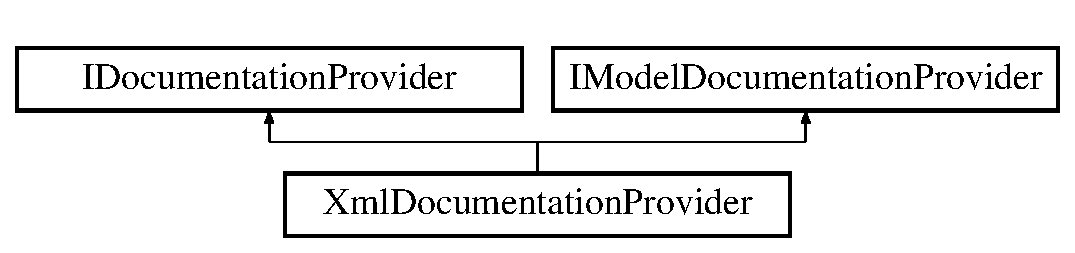
\includegraphics[height=2.000000cm]{df/d7d/classApi3Layers_1_1Areas_1_1HelpPage_1_1XmlDocumentationProvider}
\end{center}
\end{figure}
\subsection*{Métodos Públicos}
\begin{DoxyCompactItemize}
\item 
\hyperlink{classApi3Layers_1_1Areas_1_1HelpPage_1_1XmlDocumentationProvider_ad2a409539874ae63a8cebe23599fc468}{Xml\+Documentation\+Provider} (string document\+Path)
\begin{DoxyCompactList}\small\item\em Initializes a new instance of the \hyperlink{classApi3Layers_1_1Areas_1_1HelpPage_1_1XmlDocumentationProvider}{Xml\+Documentation\+Provider} class. \end{DoxyCompactList}\item 
string \hyperlink{classApi3Layers_1_1Areas_1_1HelpPage_1_1XmlDocumentationProvider_a6bf162425448d82a33aa596c66c807e0}{Get\+Documentation} (Http\+Controller\+Descriptor controller\+Descriptor)
\item 
virtual string \hyperlink{classApi3Layers_1_1Areas_1_1HelpPage_1_1XmlDocumentationProvider_aaa833c04f0d8aecd147d9755e20106e2}{Get\+Documentation} (Http\+Action\+Descriptor action\+Descriptor)
\item 
virtual string \hyperlink{classApi3Layers_1_1Areas_1_1HelpPage_1_1XmlDocumentationProvider_a7222394a33fd0f7cf2117e37d7e43dc3}{Get\+Documentation} (Http\+Parameter\+Descriptor parameter\+Descriptor)
\item 
string \hyperlink{classApi3Layers_1_1Areas_1_1HelpPage_1_1XmlDocumentationProvider_aa774bb352a769421583abb335a1cec8a}{Get\+Documentation} (Member\+Info member)
\item 
string \hyperlink{classApi3Layers_1_1Areas_1_1HelpPage_1_1XmlDocumentationProvider_af771cd863288942e506d28447daf4f82}{Get\+Documentation} (Type type)
\item 
string \hyperlink{classApi3Layers_1_1Areas_1_1HelpPage_1_1XmlDocumentationProvider_a418513d2d192474340e81271a0b4ca5f}{Get\+Response\+Documentation} (Http\+Action\+Descriptor action\+Descriptor)
\end{DoxyCompactItemize}
\subsection*{Métodos Privados}
\begin{DoxyCompactItemize}
\item 
X\+Path\+Navigator \hyperlink{classApi3Layers_1_1Areas_1_1HelpPage_1_1XmlDocumentationProvider_ada0fcccbdb5b3153540e07182fe9179a}{Get\+Method\+Node} (Http\+Action\+Descriptor action\+Descriptor)
\item 
X\+Path\+Navigator \hyperlink{classApi3Layers_1_1Areas_1_1HelpPage_1_1XmlDocumentationProvider_a8db80d23eb6731ae9ed3e9f1bde27440}{Get\+Type\+Node} (Type type)
\end{DoxyCompactItemize}
\subsection*{Métodos Privados Estáticos}
\begin{DoxyCompactItemize}
\item 
static string \hyperlink{classApi3Layers_1_1Areas_1_1HelpPage_1_1XmlDocumentationProvider_aa747494e379de7a28d7e26920b30488c}{Get\+Member\+Name} (Method\+Info method)
\item 
static string \hyperlink{classApi3Layers_1_1Areas_1_1HelpPage_1_1XmlDocumentationProvider_a0e1628e2c68deb872bb816907d1ceab1}{Get\+Tag\+Value} (X\+Path\+Navigator parent\+Node, string tag\+Name)
\item 
static string \hyperlink{classApi3Layers_1_1Areas_1_1HelpPage_1_1XmlDocumentationProvider_ab7c2e772873d333e72ee649dddacc8e9}{Get\+Type\+Name} (Type type)
\end{DoxyCompactItemize}
\subsection*{Atributos Privados}
\begin{DoxyCompactItemize}
\item 
X\+Path\+Navigator \hyperlink{classApi3Layers_1_1Areas_1_1HelpPage_1_1XmlDocumentationProvider_a27bb462cb0252e12db3c94eb7cde784a}{\+\_\+document\+Navigator}
\item 
const string \hyperlink{classApi3Layers_1_1Areas_1_1HelpPage_1_1XmlDocumentationProvider_a495fb5f073620815f4bd9be5ac5a1c31}{Field\+Expression} = \char`\"{}/doc/members/member\mbox{[}@name=\textquotesingle{}F\+:\{0\}\textquotesingle{}\mbox{]}\char`\"{}
\item 
const string \hyperlink{classApi3Layers_1_1Areas_1_1HelpPage_1_1XmlDocumentationProvider_a8e2836494bbc0eef86c4200c2daaa489}{Method\+Expression} = \char`\"{}/doc/members/member\mbox{[}@name=\textquotesingle{}M\+:\{0\}\textquotesingle{}\mbox{]}\char`\"{}
\item 
const string \hyperlink{classApi3Layers_1_1Areas_1_1HelpPage_1_1XmlDocumentationProvider_a028743d93d156432c6d394821e2596dc}{Parameter\+Expression} = \char`\"{}param\mbox{[}@name=\textquotesingle{}\{0\}\textquotesingle{}\mbox{]}\char`\"{}
\item 
const string \hyperlink{classApi3Layers_1_1Areas_1_1HelpPage_1_1XmlDocumentationProvider_ae05dc5cbd300573ef5589d577745bf33}{Property\+Expression} = \char`\"{}/doc/members/member\mbox{[}@name=\textquotesingle{}P\+:\{0\}\textquotesingle{}\mbox{]}\char`\"{}
\item 
const string \hyperlink{classApi3Layers_1_1Areas_1_1HelpPage_1_1XmlDocumentationProvider_ae421a9b71e4e2b01b648d002549328f7}{Type\+Expression} = \char`\"{}/doc/members/member\mbox{[}@name=\textquotesingle{}T\+:\{0\}\textquotesingle{}\mbox{]}\char`\"{}
\end{DoxyCompactItemize}


\subsection{Descrição Detalhada}
A custom I\+Documentation\+Provider that reads the A\+PI documentation from an X\+ML documentation file. 



\subsection{Construtores \& Destrutores}
\mbox{\Hypertarget{classApi3Layers_1_1Areas_1_1HelpPage_1_1XmlDocumentationProvider_ad2a409539874ae63a8cebe23599fc468}\label{classApi3Layers_1_1Areas_1_1HelpPage_1_1XmlDocumentationProvider_ad2a409539874ae63a8cebe23599fc468}} 
\index{Api3\+Layers\+::\+Areas\+::\+Help\+Page\+::\+Xml\+Documentation\+Provider@{Api3\+Layers\+::\+Areas\+::\+Help\+Page\+::\+Xml\+Documentation\+Provider}!Xml\+Documentation\+Provider@{Xml\+Documentation\+Provider}}
\index{Xml\+Documentation\+Provider@{Xml\+Documentation\+Provider}!Api3\+Layers\+::\+Areas\+::\+Help\+Page\+::\+Xml\+Documentation\+Provider@{Api3\+Layers\+::\+Areas\+::\+Help\+Page\+::\+Xml\+Documentation\+Provider}}
\subsubsection{\texorpdfstring{Xml\+Documentation\+Provider()}{XmlDocumentationProvider()}}
{\footnotesize\ttfamily \hyperlink{classApi3Layers_1_1Areas_1_1HelpPage_1_1XmlDocumentationProvider}{Xml\+Documentation\+Provider} (\begin{DoxyParamCaption}\item[{string}]{document\+Path }\end{DoxyParamCaption})}



Initializes a new instance of the \hyperlink{classApi3Layers_1_1Areas_1_1HelpPage_1_1XmlDocumentationProvider}{Xml\+Documentation\+Provider} class. 


\begin{DoxyParams}{Parâmetros}
{\em document\+Path} & The physical path to X\+ML document.\\
\hline
\end{DoxyParams}


\subsection{Métodos}
\mbox{\Hypertarget{classApi3Layers_1_1Areas_1_1HelpPage_1_1XmlDocumentationProvider_a6bf162425448d82a33aa596c66c807e0}\label{classApi3Layers_1_1Areas_1_1HelpPage_1_1XmlDocumentationProvider_a6bf162425448d82a33aa596c66c807e0}} 
\index{Api3\+Layers\+::\+Areas\+::\+Help\+Page\+::\+Xml\+Documentation\+Provider@{Api3\+Layers\+::\+Areas\+::\+Help\+Page\+::\+Xml\+Documentation\+Provider}!Get\+Documentation@{Get\+Documentation}}
\index{Get\+Documentation@{Get\+Documentation}!Api3\+Layers\+::\+Areas\+::\+Help\+Page\+::\+Xml\+Documentation\+Provider@{Api3\+Layers\+::\+Areas\+::\+Help\+Page\+::\+Xml\+Documentation\+Provider}}
\subsubsection{\texorpdfstring{Get\+Documentation()}{GetDocumentation()}\hspace{0.1cm}{\footnotesize\ttfamily [1/5]}}
{\footnotesize\ttfamily string Get\+Documentation (\begin{DoxyParamCaption}\item[{Http\+Controller\+Descriptor}]{controller\+Descriptor }\end{DoxyParamCaption})}

\mbox{\Hypertarget{classApi3Layers_1_1Areas_1_1HelpPage_1_1XmlDocumentationProvider_aaa833c04f0d8aecd147d9755e20106e2}\label{classApi3Layers_1_1Areas_1_1HelpPage_1_1XmlDocumentationProvider_aaa833c04f0d8aecd147d9755e20106e2}} 
\index{Api3\+Layers\+::\+Areas\+::\+Help\+Page\+::\+Xml\+Documentation\+Provider@{Api3\+Layers\+::\+Areas\+::\+Help\+Page\+::\+Xml\+Documentation\+Provider}!Get\+Documentation@{Get\+Documentation}}
\index{Get\+Documentation@{Get\+Documentation}!Api3\+Layers\+::\+Areas\+::\+Help\+Page\+::\+Xml\+Documentation\+Provider@{Api3\+Layers\+::\+Areas\+::\+Help\+Page\+::\+Xml\+Documentation\+Provider}}
\subsubsection{\texorpdfstring{Get\+Documentation()}{GetDocumentation()}\hspace{0.1cm}{\footnotesize\ttfamily [2/5]}}
{\footnotesize\ttfamily virtual string Get\+Documentation (\begin{DoxyParamCaption}\item[{Http\+Action\+Descriptor}]{action\+Descriptor }\end{DoxyParamCaption})\hspace{0.3cm}{\ttfamily [virtual]}}

\mbox{\Hypertarget{classApi3Layers_1_1Areas_1_1HelpPage_1_1XmlDocumentationProvider_a7222394a33fd0f7cf2117e37d7e43dc3}\label{classApi3Layers_1_1Areas_1_1HelpPage_1_1XmlDocumentationProvider_a7222394a33fd0f7cf2117e37d7e43dc3}} 
\index{Api3\+Layers\+::\+Areas\+::\+Help\+Page\+::\+Xml\+Documentation\+Provider@{Api3\+Layers\+::\+Areas\+::\+Help\+Page\+::\+Xml\+Documentation\+Provider}!Get\+Documentation@{Get\+Documentation}}
\index{Get\+Documentation@{Get\+Documentation}!Api3\+Layers\+::\+Areas\+::\+Help\+Page\+::\+Xml\+Documentation\+Provider@{Api3\+Layers\+::\+Areas\+::\+Help\+Page\+::\+Xml\+Documentation\+Provider}}
\subsubsection{\texorpdfstring{Get\+Documentation()}{GetDocumentation()}\hspace{0.1cm}{\footnotesize\ttfamily [3/5]}}
{\footnotesize\ttfamily virtual string Get\+Documentation (\begin{DoxyParamCaption}\item[{Http\+Parameter\+Descriptor}]{parameter\+Descriptor }\end{DoxyParamCaption})\hspace{0.3cm}{\ttfamily [virtual]}}

\mbox{\Hypertarget{classApi3Layers_1_1Areas_1_1HelpPage_1_1XmlDocumentationProvider_aa774bb352a769421583abb335a1cec8a}\label{classApi3Layers_1_1Areas_1_1HelpPage_1_1XmlDocumentationProvider_aa774bb352a769421583abb335a1cec8a}} 
\index{Api3\+Layers\+::\+Areas\+::\+Help\+Page\+::\+Xml\+Documentation\+Provider@{Api3\+Layers\+::\+Areas\+::\+Help\+Page\+::\+Xml\+Documentation\+Provider}!Get\+Documentation@{Get\+Documentation}}
\index{Get\+Documentation@{Get\+Documentation}!Api3\+Layers\+::\+Areas\+::\+Help\+Page\+::\+Xml\+Documentation\+Provider@{Api3\+Layers\+::\+Areas\+::\+Help\+Page\+::\+Xml\+Documentation\+Provider}}
\subsubsection{\texorpdfstring{Get\+Documentation()}{GetDocumentation()}\hspace{0.1cm}{\footnotesize\ttfamily [4/5]}}
{\footnotesize\ttfamily string Get\+Documentation (\begin{DoxyParamCaption}\item[{Member\+Info}]{member }\end{DoxyParamCaption})}



Implementa \hyperlink{interfaceApi3Layers_1_1Areas_1_1HelpPage_1_1ModelDescriptions_1_1IModelDocumentationProvider_aa774bb352a769421583abb335a1cec8a}{I\+Model\+Documentation\+Provider}.

\mbox{\Hypertarget{classApi3Layers_1_1Areas_1_1HelpPage_1_1XmlDocumentationProvider_af771cd863288942e506d28447daf4f82}\label{classApi3Layers_1_1Areas_1_1HelpPage_1_1XmlDocumentationProvider_af771cd863288942e506d28447daf4f82}} 
\index{Api3\+Layers\+::\+Areas\+::\+Help\+Page\+::\+Xml\+Documentation\+Provider@{Api3\+Layers\+::\+Areas\+::\+Help\+Page\+::\+Xml\+Documentation\+Provider}!Get\+Documentation@{Get\+Documentation}}
\index{Get\+Documentation@{Get\+Documentation}!Api3\+Layers\+::\+Areas\+::\+Help\+Page\+::\+Xml\+Documentation\+Provider@{Api3\+Layers\+::\+Areas\+::\+Help\+Page\+::\+Xml\+Documentation\+Provider}}
\subsubsection{\texorpdfstring{Get\+Documentation()}{GetDocumentation()}\hspace{0.1cm}{\footnotesize\ttfamily [5/5]}}
{\footnotesize\ttfamily string Get\+Documentation (\begin{DoxyParamCaption}\item[{Type}]{type }\end{DoxyParamCaption})}



Implementa \hyperlink{interfaceApi3Layers_1_1Areas_1_1HelpPage_1_1ModelDescriptions_1_1IModelDocumentationProvider_af771cd863288942e506d28447daf4f82}{I\+Model\+Documentation\+Provider}.

\mbox{\Hypertarget{classApi3Layers_1_1Areas_1_1HelpPage_1_1XmlDocumentationProvider_aa747494e379de7a28d7e26920b30488c}\label{classApi3Layers_1_1Areas_1_1HelpPage_1_1XmlDocumentationProvider_aa747494e379de7a28d7e26920b30488c}} 
\index{Api3\+Layers\+::\+Areas\+::\+Help\+Page\+::\+Xml\+Documentation\+Provider@{Api3\+Layers\+::\+Areas\+::\+Help\+Page\+::\+Xml\+Documentation\+Provider}!Get\+Member\+Name@{Get\+Member\+Name}}
\index{Get\+Member\+Name@{Get\+Member\+Name}!Api3\+Layers\+::\+Areas\+::\+Help\+Page\+::\+Xml\+Documentation\+Provider@{Api3\+Layers\+::\+Areas\+::\+Help\+Page\+::\+Xml\+Documentation\+Provider}}
\subsubsection{\texorpdfstring{Get\+Member\+Name()}{GetMemberName()}}
{\footnotesize\ttfamily static string Get\+Member\+Name (\begin{DoxyParamCaption}\item[{Method\+Info}]{method }\end{DoxyParamCaption})\hspace{0.3cm}{\ttfamily [static]}, {\ttfamily [private]}}

\mbox{\Hypertarget{classApi3Layers_1_1Areas_1_1HelpPage_1_1XmlDocumentationProvider_ada0fcccbdb5b3153540e07182fe9179a}\label{classApi3Layers_1_1Areas_1_1HelpPage_1_1XmlDocumentationProvider_ada0fcccbdb5b3153540e07182fe9179a}} 
\index{Api3\+Layers\+::\+Areas\+::\+Help\+Page\+::\+Xml\+Documentation\+Provider@{Api3\+Layers\+::\+Areas\+::\+Help\+Page\+::\+Xml\+Documentation\+Provider}!Get\+Method\+Node@{Get\+Method\+Node}}
\index{Get\+Method\+Node@{Get\+Method\+Node}!Api3\+Layers\+::\+Areas\+::\+Help\+Page\+::\+Xml\+Documentation\+Provider@{Api3\+Layers\+::\+Areas\+::\+Help\+Page\+::\+Xml\+Documentation\+Provider}}
\subsubsection{\texorpdfstring{Get\+Method\+Node()}{GetMethodNode()}}
{\footnotesize\ttfamily X\+Path\+Navigator Get\+Method\+Node (\begin{DoxyParamCaption}\item[{Http\+Action\+Descriptor}]{action\+Descriptor }\end{DoxyParamCaption})\hspace{0.3cm}{\ttfamily [private]}}

\mbox{\Hypertarget{classApi3Layers_1_1Areas_1_1HelpPage_1_1XmlDocumentationProvider_a418513d2d192474340e81271a0b4ca5f}\label{classApi3Layers_1_1Areas_1_1HelpPage_1_1XmlDocumentationProvider_a418513d2d192474340e81271a0b4ca5f}} 
\index{Api3\+Layers\+::\+Areas\+::\+Help\+Page\+::\+Xml\+Documentation\+Provider@{Api3\+Layers\+::\+Areas\+::\+Help\+Page\+::\+Xml\+Documentation\+Provider}!Get\+Response\+Documentation@{Get\+Response\+Documentation}}
\index{Get\+Response\+Documentation@{Get\+Response\+Documentation}!Api3\+Layers\+::\+Areas\+::\+Help\+Page\+::\+Xml\+Documentation\+Provider@{Api3\+Layers\+::\+Areas\+::\+Help\+Page\+::\+Xml\+Documentation\+Provider}}
\subsubsection{\texorpdfstring{Get\+Response\+Documentation()}{GetResponseDocumentation()}}
{\footnotesize\ttfamily string Get\+Response\+Documentation (\begin{DoxyParamCaption}\item[{Http\+Action\+Descriptor}]{action\+Descriptor }\end{DoxyParamCaption})}

\mbox{\Hypertarget{classApi3Layers_1_1Areas_1_1HelpPage_1_1XmlDocumentationProvider_a0e1628e2c68deb872bb816907d1ceab1}\label{classApi3Layers_1_1Areas_1_1HelpPage_1_1XmlDocumentationProvider_a0e1628e2c68deb872bb816907d1ceab1}} 
\index{Api3\+Layers\+::\+Areas\+::\+Help\+Page\+::\+Xml\+Documentation\+Provider@{Api3\+Layers\+::\+Areas\+::\+Help\+Page\+::\+Xml\+Documentation\+Provider}!Get\+Tag\+Value@{Get\+Tag\+Value}}
\index{Get\+Tag\+Value@{Get\+Tag\+Value}!Api3\+Layers\+::\+Areas\+::\+Help\+Page\+::\+Xml\+Documentation\+Provider@{Api3\+Layers\+::\+Areas\+::\+Help\+Page\+::\+Xml\+Documentation\+Provider}}
\subsubsection{\texorpdfstring{Get\+Tag\+Value()}{GetTagValue()}}
{\footnotesize\ttfamily static string Get\+Tag\+Value (\begin{DoxyParamCaption}\item[{X\+Path\+Navigator}]{parent\+Node,  }\item[{string}]{tag\+Name }\end{DoxyParamCaption})\hspace{0.3cm}{\ttfamily [static]}, {\ttfamily [private]}}

\mbox{\Hypertarget{classApi3Layers_1_1Areas_1_1HelpPage_1_1XmlDocumentationProvider_ab7c2e772873d333e72ee649dddacc8e9}\label{classApi3Layers_1_1Areas_1_1HelpPage_1_1XmlDocumentationProvider_ab7c2e772873d333e72ee649dddacc8e9}} 
\index{Api3\+Layers\+::\+Areas\+::\+Help\+Page\+::\+Xml\+Documentation\+Provider@{Api3\+Layers\+::\+Areas\+::\+Help\+Page\+::\+Xml\+Documentation\+Provider}!Get\+Type\+Name@{Get\+Type\+Name}}
\index{Get\+Type\+Name@{Get\+Type\+Name}!Api3\+Layers\+::\+Areas\+::\+Help\+Page\+::\+Xml\+Documentation\+Provider@{Api3\+Layers\+::\+Areas\+::\+Help\+Page\+::\+Xml\+Documentation\+Provider}}
\subsubsection{\texorpdfstring{Get\+Type\+Name()}{GetTypeName()}}
{\footnotesize\ttfamily static string Get\+Type\+Name (\begin{DoxyParamCaption}\item[{Type}]{type }\end{DoxyParamCaption})\hspace{0.3cm}{\ttfamily [static]}, {\ttfamily [private]}}

\mbox{\Hypertarget{classApi3Layers_1_1Areas_1_1HelpPage_1_1XmlDocumentationProvider_a8db80d23eb6731ae9ed3e9f1bde27440}\label{classApi3Layers_1_1Areas_1_1HelpPage_1_1XmlDocumentationProvider_a8db80d23eb6731ae9ed3e9f1bde27440}} 
\index{Api3\+Layers\+::\+Areas\+::\+Help\+Page\+::\+Xml\+Documentation\+Provider@{Api3\+Layers\+::\+Areas\+::\+Help\+Page\+::\+Xml\+Documentation\+Provider}!Get\+Type\+Node@{Get\+Type\+Node}}
\index{Get\+Type\+Node@{Get\+Type\+Node}!Api3\+Layers\+::\+Areas\+::\+Help\+Page\+::\+Xml\+Documentation\+Provider@{Api3\+Layers\+::\+Areas\+::\+Help\+Page\+::\+Xml\+Documentation\+Provider}}
\subsubsection{\texorpdfstring{Get\+Type\+Node()}{GetTypeNode()}}
{\footnotesize\ttfamily X\+Path\+Navigator Get\+Type\+Node (\begin{DoxyParamCaption}\item[{Type}]{type }\end{DoxyParamCaption})\hspace{0.3cm}{\ttfamily [private]}}



\subsection{Atributos}
\mbox{\Hypertarget{classApi3Layers_1_1Areas_1_1HelpPage_1_1XmlDocumentationProvider_a27bb462cb0252e12db3c94eb7cde784a}\label{classApi3Layers_1_1Areas_1_1HelpPage_1_1XmlDocumentationProvider_a27bb462cb0252e12db3c94eb7cde784a}} 
\index{Api3\+Layers\+::\+Areas\+::\+Help\+Page\+::\+Xml\+Documentation\+Provider@{Api3\+Layers\+::\+Areas\+::\+Help\+Page\+::\+Xml\+Documentation\+Provider}!\+\_\+document\+Navigator@{\+\_\+document\+Navigator}}
\index{\+\_\+document\+Navigator@{\+\_\+document\+Navigator}!Api3\+Layers\+::\+Areas\+::\+Help\+Page\+::\+Xml\+Documentation\+Provider@{Api3\+Layers\+::\+Areas\+::\+Help\+Page\+::\+Xml\+Documentation\+Provider}}
\subsubsection{\texorpdfstring{\+\_\+document\+Navigator}{\_documentNavigator}}
{\footnotesize\ttfamily X\+Path\+Navigator \+\_\+document\+Navigator\hspace{0.3cm}{\ttfamily [private]}}

\mbox{\Hypertarget{classApi3Layers_1_1Areas_1_1HelpPage_1_1XmlDocumentationProvider_a495fb5f073620815f4bd9be5ac5a1c31}\label{classApi3Layers_1_1Areas_1_1HelpPage_1_1XmlDocumentationProvider_a495fb5f073620815f4bd9be5ac5a1c31}} 
\index{Api3\+Layers\+::\+Areas\+::\+Help\+Page\+::\+Xml\+Documentation\+Provider@{Api3\+Layers\+::\+Areas\+::\+Help\+Page\+::\+Xml\+Documentation\+Provider}!Field\+Expression@{Field\+Expression}}
\index{Field\+Expression@{Field\+Expression}!Api3\+Layers\+::\+Areas\+::\+Help\+Page\+::\+Xml\+Documentation\+Provider@{Api3\+Layers\+::\+Areas\+::\+Help\+Page\+::\+Xml\+Documentation\+Provider}}
\subsubsection{\texorpdfstring{Field\+Expression}{FieldExpression}}
{\footnotesize\ttfamily const string Field\+Expression = \char`\"{}/doc/members/member\mbox{[}@name=\textquotesingle{}F\+:\{0\}\textquotesingle{}\mbox{]}\char`\"{}\hspace{0.3cm}{\ttfamily [private]}}

\mbox{\Hypertarget{classApi3Layers_1_1Areas_1_1HelpPage_1_1XmlDocumentationProvider_a8e2836494bbc0eef86c4200c2daaa489}\label{classApi3Layers_1_1Areas_1_1HelpPage_1_1XmlDocumentationProvider_a8e2836494bbc0eef86c4200c2daaa489}} 
\index{Api3\+Layers\+::\+Areas\+::\+Help\+Page\+::\+Xml\+Documentation\+Provider@{Api3\+Layers\+::\+Areas\+::\+Help\+Page\+::\+Xml\+Documentation\+Provider}!Method\+Expression@{Method\+Expression}}
\index{Method\+Expression@{Method\+Expression}!Api3\+Layers\+::\+Areas\+::\+Help\+Page\+::\+Xml\+Documentation\+Provider@{Api3\+Layers\+::\+Areas\+::\+Help\+Page\+::\+Xml\+Documentation\+Provider}}
\subsubsection{\texorpdfstring{Method\+Expression}{MethodExpression}}
{\footnotesize\ttfamily const string Method\+Expression = \char`\"{}/doc/members/member\mbox{[}@name=\textquotesingle{}M\+:\{0\}\textquotesingle{}\mbox{]}\char`\"{}\hspace{0.3cm}{\ttfamily [private]}}

\mbox{\Hypertarget{classApi3Layers_1_1Areas_1_1HelpPage_1_1XmlDocumentationProvider_a028743d93d156432c6d394821e2596dc}\label{classApi3Layers_1_1Areas_1_1HelpPage_1_1XmlDocumentationProvider_a028743d93d156432c6d394821e2596dc}} 
\index{Api3\+Layers\+::\+Areas\+::\+Help\+Page\+::\+Xml\+Documentation\+Provider@{Api3\+Layers\+::\+Areas\+::\+Help\+Page\+::\+Xml\+Documentation\+Provider}!Parameter\+Expression@{Parameter\+Expression}}
\index{Parameter\+Expression@{Parameter\+Expression}!Api3\+Layers\+::\+Areas\+::\+Help\+Page\+::\+Xml\+Documentation\+Provider@{Api3\+Layers\+::\+Areas\+::\+Help\+Page\+::\+Xml\+Documentation\+Provider}}
\subsubsection{\texorpdfstring{Parameter\+Expression}{ParameterExpression}}
{\footnotesize\ttfamily const string Parameter\+Expression = \char`\"{}param\mbox{[}@name=\textquotesingle{}\{0\}\textquotesingle{}\mbox{]}\char`\"{}\hspace{0.3cm}{\ttfamily [private]}}

\mbox{\Hypertarget{classApi3Layers_1_1Areas_1_1HelpPage_1_1XmlDocumentationProvider_ae05dc5cbd300573ef5589d577745bf33}\label{classApi3Layers_1_1Areas_1_1HelpPage_1_1XmlDocumentationProvider_ae05dc5cbd300573ef5589d577745bf33}} 
\index{Api3\+Layers\+::\+Areas\+::\+Help\+Page\+::\+Xml\+Documentation\+Provider@{Api3\+Layers\+::\+Areas\+::\+Help\+Page\+::\+Xml\+Documentation\+Provider}!Property\+Expression@{Property\+Expression}}
\index{Property\+Expression@{Property\+Expression}!Api3\+Layers\+::\+Areas\+::\+Help\+Page\+::\+Xml\+Documentation\+Provider@{Api3\+Layers\+::\+Areas\+::\+Help\+Page\+::\+Xml\+Documentation\+Provider}}
\subsubsection{\texorpdfstring{Property\+Expression}{PropertyExpression}}
{\footnotesize\ttfamily const string Property\+Expression = \char`\"{}/doc/members/member\mbox{[}@name=\textquotesingle{}P\+:\{0\}\textquotesingle{}\mbox{]}\char`\"{}\hspace{0.3cm}{\ttfamily [private]}}

\mbox{\Hypertarget{classApi3Layers_1_1Areas_1_1HelpPage_1_1XmlDocumentationProvider_ae421a9b71e4e2b01b648d002549328f7}\label{classApi3Layers_1_1Areas_1_1HelpPage_1_1XmlDocumentationProvider_ae421a9b71e4e2b01b648d002549328f7}} 
\index{Api3\+Layers\+::\+Areas\+::\+Help\+Page\+::\+Xml\+Documentation\+Provider@{Api3\+Layers\+::\+Areas\+::\+Help\+Page\+::\+Xml\+Documentation\+Provider}!Type\+Expression@{Type\+Expression}}
\index{Type\+Expression@{Type\+Expression}!Api3\+Layers\+::\+Areas\+::\+Help\+Page\+::\+Xml\+Documentation\+Provider@{Api3\+Layers\+::\+Areas\+::\+Help\+Page\+::\+Xml\+Documentation\+Provider}}
\subsubsection{\texorpdfstring{Type\+Expression}{TypeExpression}}
{\footnotesize\ttfamily const string Type\+Expression = \char`\"{}/doc/members/member\mbox{[}@name=\textquotesingle{}T\+:\{0\}\textquotesingle{}\mbox{]}\char`\"{}\hspace{0.3cm}{\ttfamily [private]}}



A documentação para esta classe foi gerada a partir do seguinte arquivo\+:\begin{DoxyCompactItemize}
\item 
C\+:/\+Users/\+Bruno/\+Desktop/\+Api3\+Layers/\+Api3\+Layers/\+Areas/\+Help\+Page/\hyperlink{XmlDocumentationProvider_8cs}{Xml\+Documentation\+Provider.\+cs}\end{DoxyCompactItemize}

\hypertarget{classApi3Layers_1_1BundleConfig}{}\section{Bundle\+Config}
\label{classApi3Layers_1_1BundleConfig}\index{Bundle\+Config@{Bundle\+Config}}
\subsection*{Métodos Públicos Estáticos}
\begin{DoxyCompactItemize}
\item 
static void \hyperlink{classApi3Layers_1_1BundleConfig_afab9ce33b79d8441026ebdfebdf1e91b}{Register\+Bundles} (Bundle\+Collection bundles)
\end{DoxyCompactItemize}


\subsection{Métodos}
\mbox{\Hypertarget{classApi3Layers_1_1BundleConfig_afab9ce33b79d8441026ebdfebdf1e91b}\label{classApi3Layers_1_1BundleConfig_afab9ce33b79d8441026ebdfebdf1e91b}} 
\index{Api3\+Layers\+::\+Bundle\+Config@{Api3\+Layers\+::\+Bundle\+Config}!Register\+Bundles@{Register\+Bundles}}
\index{Register\+Bundles@{Register\+Bundles}!Api3\+Layers\+::\+Bundle\+Config@{Api3\+Layers\+::\+Bundle\+Config}}
\subsubsection{\texorpdfstring{Register\+Bundles()}{RegisterBundles()}}
{\footnotesize\ttfamily static void Register\+Bundles (\begin{DoxyParamCaption}\item[{Bundle\+Collection}]{bundles }\end{DoxyParamCaption})\hspace{0.3cm}{\ttfamily [static]}}



A documentação para esta classe foi gerada a partir do seguinte arquivo\+:\begin{DoxyCompactItemize}
\item 
C\+:/\+Users/\+Bruno/\+Desktop/\+Api3\+Layers/\+Api3\+Layers/\+App\+\_\+\+Start/\hyperlink{BundleConfig_8cs}{Bundle\+Config.\+cs}\end{DoxyCompactItemize}

\hypertarget{classApi3Layers_1_1Controllers_1_1ClientController}{}\section{Client\+Controller}
\label{classApi3Layers_1_1Controllers_1_1ClientController}\index{Client\+Controller@{Client\+Controller}}
Diagrama de Hierarquia para Client\+Controller\+:\begin{figure}[H]
\begin{center}
\leavevmode
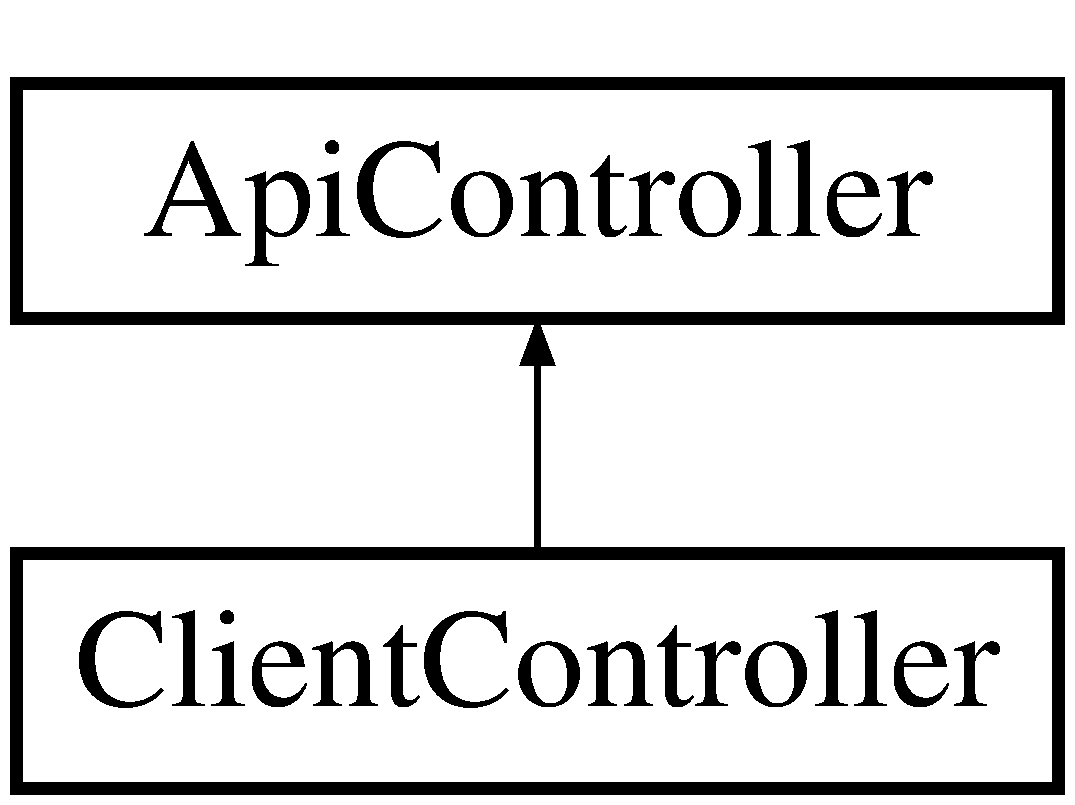
\includegraphics[height=2.000000cm]{d6/d89/classApi3Layers_1_1Controllers_1_1ClientController}
\end{center}
\end{figure}
\subsection*{Métodos Públicos}
\begin{DoxyCompactItemize}
\item 
Task$<$ Http\+Response\+Message $>$ \hyperlink{classApi3Layers_1_1Controllers_1_1ClientController_a9313f9369acc70d20109a5e2621486fd}{Delete\+Client} (Client client)
\item 
Task$<$ Http\+Response\+Message $>$ \hyperlink{classApi3Layers_1_1Controllers_1_1ClientController_a63543b21b5d71a250f5c2e251e1725eb}{getby\+ID} (int id)
\item 
Task$<$ Http\+Response\+Message $>$ \hyperlink{classApi3Layers_1_1Controllers_1_1ClientController_a6d76d1f7034cfdf7e36f0b2f47c61019}{getby\+Name} (string name)
\item 
Task$<$ Http\+Response\+Message $>$ \hyperlink{classApi3Layers_1_1Controllers_1_1ClientController_acd6322615b0779aafdbef5f44517f329}{get\+Clients} (Client client)
\item 
Task$<$ Http\+Response\+Message $>$ \hyperlink{classApi3Layers_1_1Controllers_1_1ClientController_a05f7ee98b8ff74ab142860e21b1f8350}{Post\+Client} (Client client)
\item 
Task$<$ Http\+Response\+Message $>$ \hyperlink{classApi3Layers_1_1Controllers_1_1ClientController_ad9896ffbab1cde391410a4685f44f0f6}{Put\+Client} (Client client)
\end{DoxyCompactItemize}
\subsection*{Atributos Privados}
\begin{DoxyCompactItemize}
\item 
Task\+Completion\+Source$<$ Http\+Response\+Message $>$ \hyperlink{classApi3Layers_1_1Controllers_1_1ClientController_a467fbe1f298526ce8f849c2cd8f8fa4e}{\+\_\+\+Complete\+Task\+Source} = new Task\+Completion\+Source$<$Http\+Response\+Message$>$()
\item 
Http\+Response\+Message \hyperlink{classApi3Layers_1_1Controllers_1_1ClientController_addf535da0da455d00a0bd7a519f618cb}{\+\_\+response} = new Http\+Response\+Message()
\end{DoxyCompactItemize}


\subsection{Métodos}
\mbox{\Hypertarget{classApi3Layers_1_1Controllers_1_1ClientController_a9313f9369acc70d20109a5e2621486fd}\label{classApi3Layers_1_1Controllers_1_1ClientController_a9313f9369acc70d20109a5e2621486fd}} 
\index{Api3\+Layers\+::\+Controllers\+::\+Client\+Controller@{Api3\+Layers\+::\+Controllers\+::\+Client\+Controller}!Delete\+Client@{Delete\+Client}}
\index{Delete\+Client@{Delete\+Client}!Api3\+Layers\+::\+Controllers\+::\+Client\+Controller@{Api3\+Layers\+::\+Controllers\+::\+Client\+Controller}}
\subsubsection{\texorpdfstring{Delete\+Client()}{DeleteClient()}}
{\footnotesize\ttfamily Task$<$Http\+Response\+Message$>$ Delete\+Client (\begin{DoxyParamCaption}\item[{Client}]{client }\end{DoxyParamCaption})}

\mbox{\Hypertarget{classApi3Layers_1_1Controllers_1_1ClientController_a63543b21b5d71a250f5c2e251e1725eb}\label{classApi3Layers_1_1Controllers_1_1ClientController_a63543b21b5d71a250f5c2e251e1725eb}} 
\index{Api3\+Layers\+::\+Controllers\+::\+Client\+Controller@{Api3\+Layers\+::\+Controllers\+::\+Client\+Controller}!getby\+ID@{getby\+ID}}
\index{getby\+ID@{getby\+ID}!Api3\+Layers\+::\+Controllers\+::\+Client\+Controller@{Api3\+Layers\+::\+Controllers\+::\+Client\+Controller}}
\subsubsection{\texorpdfstring{getby\+I\+D()}{getbyID()}}
{\footnotesize\ttfamily Task$<$Http\+Response\+Message$>$ getby\+ID (\begin{DoxyParamCaption}\item[{int}]{id }\end{DoxyParamCaption})}

\mbox{\Hypertarget{classApi3Layers_1_1Controllers_1_1ClientController_a6d76d1f7034cfdf7e36f0b2f47c61019}\label{classApi3Layers_1_1Controllers_1_1ClientController_a6d76d1f7034cfdf7e36f0b2f47c61019}} 
\index{Api3\+Layers\+::\+Controllers\+::\+Client\+Controller@{Api3\+Layers\+::\+Controllers\+::\+Client\+Controller}!getby\+Name@{getby\+Name}}
\index{getby\+Name@{getby\+Name}!Api3\+Layers\+::\+Controllers\+::\+Client\+Controller@{Api3\+Layers\+::\+Controllers\+::\+Client\+Controller}}
\subsubsection{\texorpdfstring{getby\+Name()}{getbyName()}}
{\footnotesize\ttfamily Task$<$Http\+Response\+Message$>$ getby\+Name (\begin{DoxyParamCaption}\item[{string}]{name }\end{DoxyParamCaption})}

\mbox{\Hypertarget{classApi3Layers_1_1Controllers_1_1ClientController_acd6322615b0779aafdbef5f44517f329}\label{classApi3Layers_1_1Controllers_1_1ClientController_acd6322615b0779aafdbef5f44517f329}} 
\index{Api3\+Layers\+::\+Controllers\+::\+Client\+Controller@{Api3\+Layers\+::\+Controllers\+::\+Client\+Controller}!get\+Clients@{get\+Clients}}
\index{get\+Clients@{get\+Clients}!Api3\+Layers\+::\+Controllers\+::\+Client\+Controller@{Api3\+Layers\+::\+Controllers\+::\+Client\+Controller}}
\subsubsection{\texorpdfstring{get\+Clients()}{getClients()}}
{\footnotesize\ttfamily Task$<$Http\+Response\+Message$>$ get\+Clients (\begin{DoxyParamCaption}\item[{Client}]{client }\end{DoxyParamCaption})}

\mbox{\Hypertarget{classApi3Layers_1_1Controllers_1_1ClientController_a05f7ee98b8ff74ab142860e21b1f8350}\label{classApi3Layers_1_1Controllers_1_1ClientController_a05f7ee98b8ff74ab142860e21b1f8350}} 
\index{Api3\+Layers\+::\+Controllers\+::\+Client\+Controller@{Api3\+Layers\+::\+Controllers\+::\+Client\+Controller}!Post\+Client@{Post\+Client}}
\index{Post\+Client@{Post\+Client}!Api3\+Layers\+::\+Controllers\+::\+Client\+Controller@{Api3\+Layers\+::\+Controllers\+::\+Client\+Controller}}
\subsubsection{\texorpdfstring{Post\+Client()}{PostClient()}}
{\footnotesize\ttfamily Task$<$Http\+Response\+Message$>$ Post\+Client (\begin{DoxyParamCaption}\item[{Client}]{client }\end{DoxyParamCaption})}

\mbox{\Hypertarget{classApi3Layers_1_1Controllers_1_1ClientController_ad9896ffbab1cde391410a4685f44f0f6}\label{classApi3Layers_1_1Controllers_1_1ClientController_ad9896ffbab1cde391410a4685f44f0f6}} 
\index{Api3\+Layers\+::\+Controllers\+::\+Client\+Controller@{Api3\+Layers\+::\+Controllers\+::\+Client\+Controller}!Put\+Client@{Put\+Client}}
\index{Put\+Client@{Put\+Client}!Api3\+Layers\+::\+Controllers\+::\+Client\+Controller@{Api3\+Layers\+::\+Controllers\+::\+Client\+Controller}}
\subsubsection{\texorpdfstring{Put\+Client()}{PutClient()}}
{\footnotesize\ttfamily Task$<$Http\+Response\+Message$>$ Put\+Client (\begin{DoxyParamCaption}\item[{Client}]{client }\end{DoxyParamCaption})}



\subsection{Atributos}
\mbox{\Hypertarget{classApi3Layers_1_1Controllers_1_1ClientController_a467fbe1f298526ce8f849c2cd8f8fa4e}\label{classApi3Layers_1_1Controllers_1_1ClientController_a467fbe1f298526ce8f849c2cd8f8fa4e}} 
\index{Api3\+Layers\+::\+Controllers\+::\+Client\+Controller@{Api3\+Layers\+::\+Controllers\+::\+Client\+Controller}!\+\_\+\+Complete\+Task\+Source@{\+\_\+\+Complete\+Task\+Source}}
\index{\+\_\+\+Complete\+Task\+Source@{\+\_\+\+Complete\+Task\+Source}!Api3\+Layers\+::\+Controllers\+::\+Client\+Controller@{Api3\+Layers\+::\+Controllers\+::\+Client\+Controller}}
\subsubsection{\texorpdfstring{\+\_\+\+Complete\+Task\+Source}{\_CompleteTaskSource}}
{\footnotesize\ttfamily Task\+Completion\+Source$<$Http\+Response\+Message$>$ \+\_\+\+Complete\+Task\+Source = new Task\+Completion\+Source$<$Http\+Response\+Message$>$()\hspace{0.3cm}{\ttfamily [private]}}

\mbox{\Hypertarget{classApi3Layers_1_1Controllers_1_1ClientController_addf535da0da455d00a0bd7a519f618cb}\label{classApi3Layers_1_1Controllers_1_1ClientController_addf535da0da455d00a0bd7a519f618cb}} 
\index{Api3\+Layers\+::\+Controllers\+::\+Client\+Controller@{Api3\+Layers\+::\+Controllers\+::\+Client\+Controller}!\+\_\+response@{\+\_\+response}}
\index{\+\_\+response@{\+\_\+response}!Api3\+Layers\+::\+Controllers\+::\+Client\+Controller@{Api3\+Layers\+::\+Controllers\+::\+Client\+Controller}}
\subsubsection{\texorpdfstring{\+\_\+response}{\_response}}
{\footnotesize\ttfamily Http\+Response\+Message \+\_\+response = new Http\+Response\+Message()\hspace{0.3cm}{\ttfamily [private]}}



A documentação para esta classe foi gerada a partir do seguinte arquivo\+:\begin{DoxyCompactItemize}
\item 
C\+:/\+Users/\+Bruno/\+Desktop/\+Api3\+Layers/\+Api3\+Layers/\+Controllers/\hyperlink{ClientController_8cs}{Client\+Controller.\+cs}\end{DoxyCompactItemize}

\hypertarget{classApi3Layers_1_1Controllers_1_1HomeController}{}\section{Home\+Controller}
\label{classApi3Layers_1_1Controllers_1_1HomeController}\index{Home\+Controller@{Home\+Controller}}
Diagrama de Hierarquia para Home\+Controller\+:\begin{figure}[H]
\begin{center}
\leavevmode
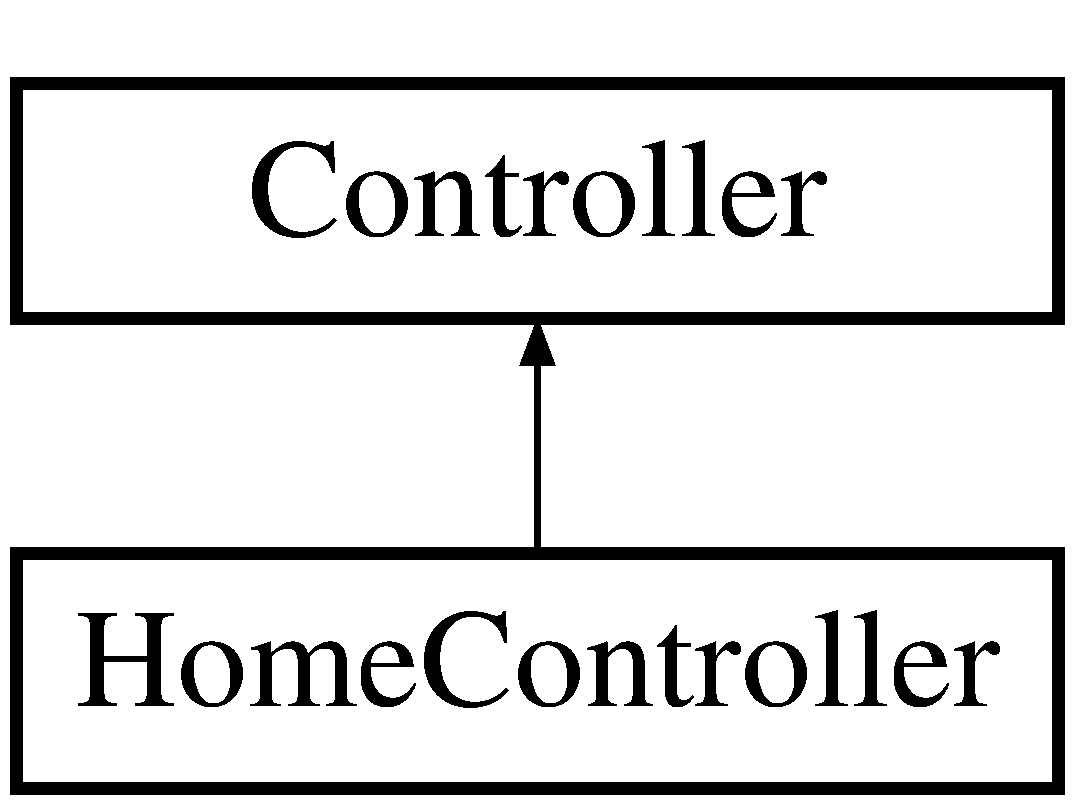
\includegraphics[height=2.000000cm]{d5/d1b/classApi3Layers_1_1Controllers_1_1HomeController}
\end{center}
\end{figure}
\subsection*{Métodos Públicos}
\begin{DoxyCompactItemize}
\item 
Action\+Result \hyperlink{classApi3Layers_1_1Controllers_1_1HomeController_a82bdd581a9c68d02c11ac8160aa5d60b}{Index} ()
\end{DoxyCompactItemize}


\subsection{Métodos}
\mbox{\Hypertarget{classApi3Layers_1_1Controllers_1_1HomeController_a82bdd581a9c68d02c11ac8160aa5d60b}\label{classApi3Layers_1_1Controllers_1_1HomeController_a82bdd581a9c68d02c11ac8160aa5d60b}} 
\index{Api3\+Layers\+::\+Controllers\+::\+Home\+Controller@{Api3\+Layers\+::\+Controllers\+::\+Home\+Controller}!Index@{Index}}
\index{Index@{Index}!Api3\+Layers\+::\+Controllers\+::\+Home\+Controller@{Api3\+Layers\+::\+Controllers\+::\+Home\+Controller}}
\subsubsection{\texorpdfstring{Index()}{Index()}}
{\footnotesize\ttfamily Action\+Result Index (\begin{DoxyParamCaption}{ }\end{DoxyParamCaption})}



A documentação para esta classe foi gerada a partir do seguinte arquivo\+:\begin{DoxyCompactItemize}
\item 
C\+:/\+Users/\+Bruno/\+Desktop/\+Api3\+Layers/\+Api3\+Layers/\+Controllers/\hyperlink{HomeController_8cs}{Home\+Controller.\+cs}\end{DoxyCompactItemize}

\hypertarget{classApi3Layers_1_1FilterConfig}{}\section{Filter\+Config}
\label{classApi3Layers_1_1FilterConfig}\index{Filter\+Config@{Filter\+Config}}
\subsection*{Métodos Públicos Estáticos}
\begin{DoxyCompactItemize}
\item 
static void \hyperlink{classApi3Layers_1_1FilterConfig_a25694cee76ca514824bd682cfc9b4ad0}{Register\+Global\+Filters} (Global\+Filter\+Collection filters)
\end{DoxyCompactItemize}


\subsection{Métodos}
\mbox{\Hypertarget{classApi3Layers_1_1FilterConfig_a25694cee76ca514824bd682cfc9b4ad0}\label{classApi3Layers_1_1FilterConfig_a25694cee76ca514824bd682cfc9b4ad0}} 
\index{Api3\+Layers\+::\+Filter\+Config@{Api3\+Layers\+::\+Filter\+Config}!Register\+Global\+Filters@{Register\+Global\+Filters}}
\index{Register\+Global\+Filters@{Register\+Global\+Filters}!Api3\+Layers\+::\+Filter\+Config@{Api3\+Layers\+::\+Filter\+Config}}
\subsubsection{\texorpdfstring{Register\+Global\+Filters()}{RegisterGlobalFilters()}}
{\footnotesize\ttfamily static void Register\+Global\+Filters (\begin{DoxyParamCaption}\item[{Global\+Filter\+Collection}]{filters }\end{DoxyParamCaption})\hspace{0.3cm}{\ttfamily [static]}}



A documentação para esta classe foi gerada a partir do seguinte arquivo\+:\begin{DoxyCompactItemize}
\item 
Api3\+Layers/\+App\+\_\+\+Start/\hyperlink{FilterConfig_8cs}{Filter\+Config.\+cs}\end{DoxyCompactItemize}

\hypertarget{classApi3Layers_1_1RouteConfig}{}\section{Route\+Config}
\label{classApi3Layers_1_1RouteConfig}\index{Route\+Config@{Route\+Config}}
\subsection*{Métodos Públicos Estáticos}
\begin{DoxyCompactItemize}
\item 
static void \hyperlink{classApi3Layers_1_1RouteConfig_a11e22f7991e945338ef5051492f404a9}{Register\+Routes} (Route\+Collection routes)
\end{DoxyCompactItemize}


\subsection{Métodos}
\mbox{\Hypertarget{classApi3Layers_1_1RouteConfig_a11e22f7991e945338ef5051492f404a9}\label{classApi3Layers_1_1RouteConfig_a11e22f7991e945338ef5051492f404a9}} 
\index{Api3\+Layers\+::\+Route\+Config@{Api3\+Layers\+::\+Route\+Config}!Register\+Routes@{Register\+Routes}}
\index{Register\+Routes@{Register\+Routes}!Api3\+Layers\+::\+Route\+Config@{Api3\+Layers\+::\+Route\+Config}}
\subsubsection{\texorpdfstring{Register\+Routes()}{RegisterRoutes()}}
{\footnotesize\ttfamily static void Register\+Routes (\begin{DoxyParamCaption}\item[{Route\+Collection}]{routes }\end{DoxyParamCaption})\hspace{0.3cm}{\ttfamily [static]}}



A documentação para esta classe foi gerada a partir do seguinte arquivo\+:\begin{DoxyCompactItemize}
\item 
C\+:/\+Users/\+Bruno/\+Desktop/\+Api3\+Layers/\+Api3\+Layers/\+App\+\_\+\+Start/\hyperlink{RouteConfig_8cs}{Route\+Config.\+cs}\end{DoxyCompactItemize}

\hypertarget{classApi3Layers_1_1WebApiApplication}{}\section{Web\+Api\+Application}
\label{classApi3Layers_1_1WebApiApplication}\index{Web\+Api\+Application@{Web\+Api\+Application}}
Diagrama de Hierarquia para Web\+Api\+Application\+:\begin{figure}[H]
\begin{center}
\leavevmode
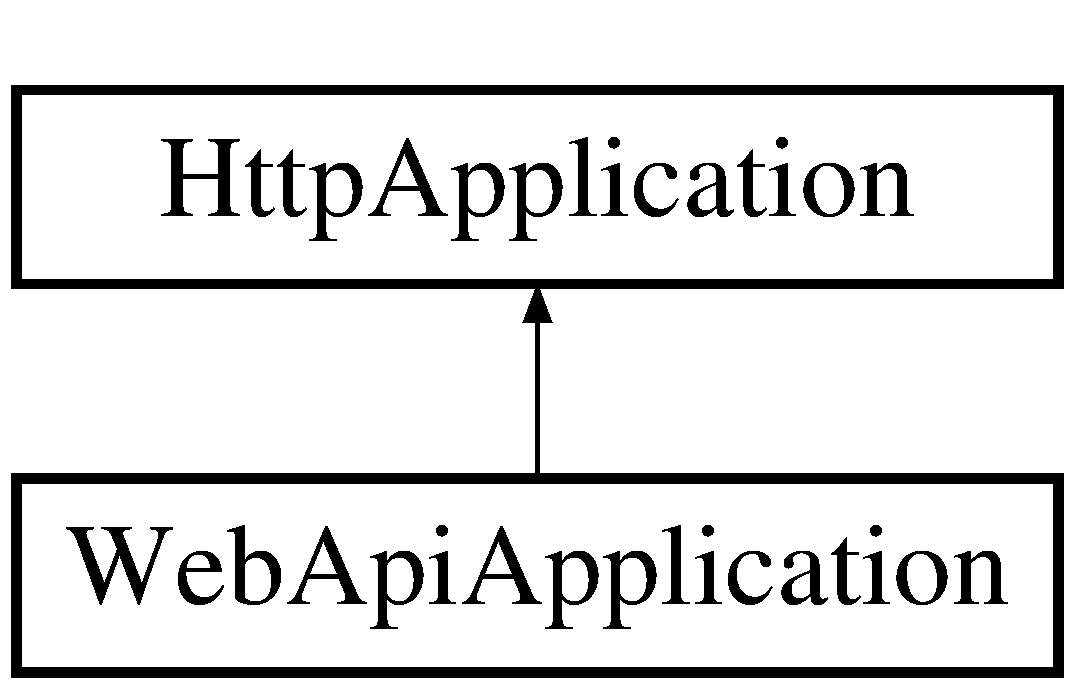
\includegraphics[height=2.000000cm]{classApi3Layers_1_1WebApiApplication}
\end{center}
\end{figure}
\subsection*{Métodos Protegidos}
\begin{DoxyCompactItemize}
\item 
void \hyperlink{classApi3Layers_1_1WebApiApplication_a71cc7d9b902e8fc085595da1960a157c}{Application\+\_\+\+Start} ()
\end{DoxyCompactItemize}


\subsection{Métodos}
\mbox{\Hypertarget{classApi3Layers_1_1WebApiApplication_a71cc7d9b902e8fc085595da1960a157c}\label{classApi3Layers_1_1WebApiApplication_a71cc7d9b902e8fc085595da1960a157c}} 
\index{Api3\+Layers\+::\+Web\+Api\+Application@{Api3\+Layers\+::\+Web\+Api\+Application}!Application\+\_\+\+Start@{Application\+\_\+\+Start}}
\index{Application\+\_\+\+Start@{Application\+\_\+\+Start}!Api3\+Layers\+::\+Web\+Api\+Application@{Api3\+Layers\+::\+Web\+Api\+Application}}
\subsubsection{\texorpdfstring{Application\+\_\+\+Start()}{Application\_Start()}}
{\footnotesize\ttfamily void Application\+\_\+\+Start (\begin{DoxyParamCaption}{ }\end{DoxyParamCaption})\hspace{0.3cm}{\ttfamily [protected]}}



A documentação para esta classe foi gerada a partir do seguinte arquivo\+:\begin{DoxyCompactItemize}
\item 
Api3\+Layers/\hyperlink{Global_8asax_8cs}{Global.\+asax.\+cs}\end{DoxyCompactItemize}

\hypertarget{classApi3Layers_1_1WebApiConfig}{}\section{Web\+Api\+Config}
\label{classApi3Layers_1_1WebApiConfig}\index{Web\+Api\+Config@{Web\+Api\+Config}}
\subsection*{Métodos Públicos Estáticos}
\begin{DoxyCompactItemize}
\item 
static void \hyperlink{classApi3Layers_1_1WebApiConfig_a8941f9a1c4d63842b463068258264cf4}{Register} (Http\+Configuration config)
\end{DoxyCompactItemize}


\subsection{Métodos}
\mbox{\Hypertarget{classApi3Layers_1_1WebApiConfig_a8941f9a1c4d63842b463068258264cf4}\label{classApi3Layers_1_1WebApiConfig_a8941f9a1c4d63842b463068258264cf4}} 
\index{Api3\+Layers\+::\+Web\+Api\+Config@{Api3\+Layers\+::\+Web\+Api\+Config}!Register@{Register}}
\index{Register@{Register}!Api3\+Layers\+::\+Web\+Api\+Config@{Api3\+Layers\+::\+Web\+Api\+Config}}
\subsubsection{\texorpdfstring{Register()}{Register()}}
{\footnotesize\ttfamily static void Register (\begin{DoxyParamCaption}\item[{Http\+Configuration}]{config }\end{DoxyParamCaption})\hspace{0.3cm}{\ttfamily [static]}}



A documentação para esta classe foi gerada a partir do seguinte arquivo\+:\begin{DoxyCompactItemize}
\item 
Api3\+Layers/\+App\+\_\+\+Start/\hyperlink{WebApiConfig_8cs}{Web\+Api\+Config.\+cs}\end{DoxyCompactItemize}

\hypertarget{classBusiness_1_1ClientBusiness}{}\section{Client\+Business}
\label{classBusiness_1_1ClientBusiness}\index{Client\+Business@{Client\+Business}}
\subsection*{Métodos Públicos}
\begin{DoxyCompactItemize}
\item 
Client \hyperlink{classBusiness_1_1ClientBusiness_afb681df27b3533da4cee4cce1eb4a548}{desactive\+Client} (Client client)
\begin{DoxyCompactList}\small\item\em Realiza as validações para desativar (excluir) um cliente \end{DoxyCompactList}\item 
Client \hyperlink{classBusiness_1_1ClientBusiness_a8342831feddce88564ead2ac46ea1550}{Validation\+Client} (Client client)
\begin{DoxyCompactList}\small\item\em Realiza as validações para inserção de ususarios \end{DoxyCompactList}\end{DoxyCompactItemize}


\subsection{Métodos}
\mbox{\Hypertarget{classBusiness_1_1ClientBusiness_afb681df27b3533da4cee4cce1eb4a548}\label{classBusiness_1_1ClientBusiness_afb681df27b3533da4cee4cce1eb4a548}} 
\index{Business\+::\+Client\+Business@{Business\+::\+Client\+Business}!desactive\+Client@{desactive\+Client}}
\index{desactive\+Client@{desactive\+Client}!Business\+::\+Client\+Business@{Business\+::\+Client\+Business}}
\subsubsection{\texorpdfstring{desactive\+Client()}{desactiveClient()}}
{\footnotesize\ttfamily Client desactive\+Client (\begin{DoxyParamCaption}\item[{Client}]{client }\end{DoxyParamCaption})}



Realiza as validações para desativar (excluir) um cliente 


\begin{DoxyParams}{Parâmetros}
{\em client} & \\
\hline
\end{DoxyParams}
\begin{DoxyReturn}{Retorna}
Client
\end{DoxyReturn}
\mbox{\Hypertarget{classBusiness_1_1ClientBusiness_a8342831feddce88564ead2ac46ea1550}\label{classBusiness_1_1ClientBusiness_a8342831feddce88564ead2ac46ea1550}} 
\index{Business\+::\+Client\+Business@{Business\+::\+Client\+Business}!Validation\+Client@{Validation\+Client}}
\index{Validation\+Client@{Validation\+Client}!Business\+::\+Client\+Business@{Business\+::\+Client\+Business}}
\subsubsection{\texorpdfstring{Validation\+Client()}{ValidationClient()}}
{\footnotesize\ttfamily Client Validation\+Client (\begin{DoxyParamCaption}\item[{Client}]{client }\end{DoxyParamCaption})}



Realiza as validações para inserção de ususarios 


\begin{DoxyParams}{Parâmetros}
{\em client} & \\
\hline
\end{DoxyParams}
\begin{DoxyReturn}{Retorna}
Client
\end{DoxyReturn}


A documentação para esta classe foi gerada a partir do seguinte arquivo\+:\begin{DoxyCompactItemize}
\item 
Business/\hyperlink{ClientBusiness_8cs}{Client\+Business.\+cs}\end{DoxyCompactItemize}

\hypertarget{interfaceDomain_1_1Interfaces_1_1IServiceBase}{}\section{I\+Service\+Base$<$ T\+Entity $>$}
\label{interfaceDomain_1_1Interfaces_1_1IServiceBase}\index{I\+Service\+Base$<$ T\+Entity $>$@{I\+Service\+Base$<$ T\+Entity $>$}}
\subsection*{Métodos Públicos}
\begin{DoxyCompactItemize}
\item 
void \hyperlink{interfaceDomain_1_1Interfaces_1_1IServiceBase_aed1520a909075057585cb4c08509840c}{Delete} (T\+Entity obj)
\item 
void \hyperlink{interfaceDomain_1_1Interfaces_1_1IServiceBase_a6e2d745cdb7a7b983f861ed6a9a541a7}{Dispose} ()
\item 
I\+Enumerable$<$ T\+Entity $>$ \hyperlink{interfaceDomain_1_1Interfaces_1_1IServiceBase_a9419e993dd7b14ea9711c035545ba3be}{Get\+All} ()
\item 
T\+Entity \hyperlink{interfaceDomain_1_1Interfaces_1_1IServiceBase_a46f8e0fa79eb922f5efbbebeb4f1788c}{Get\+By\+Id} (int id)
\item 
void \hyperlink{interfaceDomain_1_1Interfaces_1_1IServiceBase_aea7b25214718d0a8e96d77c8ee91da54}{insert} (T\+Entity obj)
\item 
void \hyperlink{interfaceDomain_1_1Interfaces_1_1IServiceBase_a6a657f225bc81497581a8919ae894bfc}{Update} (T\+Entity obj)
\end{DoxyCompactItemize}


\subsection{Métodos}
\mbox{\Hypertarget{interfaceDomain_1_1Interfaces_1_1IServiceBase_aed1520a909075057585cb4c08509840c}\label{interfaceDomain_1_1Interfaces_1_1IServiceBase_aed1520a909075057585cb4c08509840c}} 
\index{Domain\+::\+Interfaces\+::\+I\+Service\+Base@{Domain\+::\+Interfaces\+::\+I\+Service\+Base}!Delete@{Delete}}
\index{Delete@{Delete}!Domain\+::\+Interfaces\+::\+I\+Service\+Base@{Domain\+::\+Interfaces\+::\+I\+Service\+Base}}
\subsubsection{\texorpdfstring{Delete()}{Delete()}}
{\footnotesize\ttfamily void Delete (\begin{DoxyParamCaption}\item[{T\+Entity}]{obj }\end{DoxyParamCaption})}

\mbox{\Hypertarget{interfaceDomain_1_1Interfaces_1_1IServiceBase_a6e2d745cdb7a7b983f861ed6a9a541a7}\label{interfaceDomain_1_1Interfaces_1_1IServiceBase_a6e2d745cdb7a7b983f861ed6a9a541a7}} 
\index{Domain\+::\+Interfaces\+::\+I\+Service\+Base@{Domain\+::\+Interfaces\+::\+I\+Service\+Base}!Dispose@{Dispose}}
\index{Dispose@{Dispose}!Domain\+::\+Interfaces\+::\+I\+Service\+Base@{Domain\+::\+Interfaces\+::\+I\+Service\+Base}}
\subsubsection{\texorpdfstring{Dispose()}{Dispose()}}
{\footnotesize\ttfamily void Dispose (\begin{DoxyParamCaption}{ }\end{DoxyParamCaption})}

\mbox{\Hypertarget{interfaceDomain_1_1Interfaces_1_1IServiceBase_a9419e993dd7b14ea9711c035545ba3be}\label{interfaceDomain_1_1Interfaces_1_1IServiceBase_a9419e993dd7b14ea9711c035545ba3be}} 
\index{Domain\+::\+Interfaces\+::\+I\+Service\+Base@{Domain\+::\+Interfaces\+::\+I\+Service\+Base}!Get\+All@{Get\+All}}
\index{Get\+All@{Get\+All}!Domain\+::\+Interfaces\+::\+I\+Service\+Base@{Domain\+::\+Interfaces\+::\+I\+Service\+Base}}
\subsubsection{\texorpdfstring{Get\+All()}{GetAll()}}
{\footnotesize\ttfamily I\+Enumerable$<$T\+Entity$>$ Get\+All (\begin{DoxyParamCaption}{ }\end{DoxyParamCaption})}

\mbox{\Hypertarget{interfaceDomain_1_1Interfaces_1_1IServiceBase_a46f8e0fa79eb922f5efbbebeb4f1788c}\label{interfaceDomain_1_1Interfaces_1_1IServiceBase_a46f8e0fa79eb922f5efbbebeb4f1788c}} 
\index{Domain\+::\+Interfaces\+::\+I\+Service\+Base@{Domain\+::\+Interfaces\+::\+I\+Service\+Base}!Get\+By\+Id@{Get\+By\+Id}}
\index{Get\+By\+Id@{Get\+By\+Id}!Domain\+::\+Interfaces\+::\+I\+Service\+Base@{Domain\+::\+Interfaces\+::\+I\+Service\+Base}}
\subsubsection{\texorpdfstring{Get\+By\+Id()}{GetById()}}
{\footnotesize\ttfamily T\+Entity Get\+By\+Id (\begin{DoxyParamCaption}\item[{int}]{id }\end{DoxyParamCaption})}

\mbox{\Hypertarget{interfaceDomain_1_1Interfaces_1_1IServiceBase_aea7b25214718d0a8e96d77c8ee91da54}\label{interfaceDomain_1_1Interfaces_1_1IServiceBase_aea7b25214718d0a8e96d77c8ee91da54}} 
\index{Domain\+::\+Interfaces\+::\+I\+Service\+Base@{Domain\+::\+Interfaces\+::\+I\+Service\+Base}!insert@{insert}}
\index{insert@{insert}!Domain\+::\+Interfaces\+::\+I\+Service\+Base@{Domain\+::\+Interfaces\+::\+I\+Service\+Base}}
\subsubsection{\texorpdfstring{insert()}{insert()}}
{\footnotesize\ttfamily void insert (\begin{DoxyParamCaption}\item[{T\+Entity}]{obj }\end{DoxyParamCaption})}

\mbox{\Hypertarget{interfaceDomain_1_1Interfaces_1_1IServiceBase_a6a657f225bc81497581a8919ae894bfc}\label{interfaceDomain_1_1Interfaces_1_1IServiceBase_a6a657f225bc81497581a8919ae894bfc}} 
\index{Domain\+::\+Interfaces\+::\+I\+Service\+Base@{Domain\+::\+Interfaces\+::\+I\+Service\+Base}!Update@{Update}}
\index{Update@{Update}!Domain\+::\+Interfaces\+::\+I\+Service\+Base@{Domain\+::\+Interfaces\+::\+I\+Service\+Base}}
\subsubsection{\texorpdfstring{Update()}{Update()}}
{\footnotesize\ttfamily void Update (\begin{DoxyParamCaption}\item[{T\+Entity}]{obj }\end{DoxyParamCaption})}



A documentação para esta interface foi gerada a partir do seguinte arquivo\+:\begin{DoxyCompactItemize}
\item 
Domain/\+Interfaces/\hyperlink{IServiceBase_8cs}{I\+Service\+Base.\+cs}\end{DoxyCompactItemize}

\chapter{Arquivos}
\hypertarget{BundleConfig_8cs}{}\section{Referência do Arquivo C\+:/\+Users/\+Bruno/\+Desktop/\+Api3\+Layers/\+Api3\+Layers/\+App\+\_\+\+Start/\+Bundle\+Config.cs}
\label{BundleConfig_8cs}\index{C\+:/\+Users/\+Bruno/\+Desktop/\+Api3\+Layers/\+Api3\+Layers/\+App\+\_\+\+Start/\+Bundle\+Config.\+cs@{C\+:/\+Users/\+Bruno/\+Desktop/\+Api3\+Layers/\+Api3\+Layers/\+App\+\_\+\+Start/\+Bundle\+Config.\+cs}}
\subsection*{Componentes}
\begin{DoxyCompactItemize}
\item 
class \hyperlink{classApi3Layers_1_1BundleConfig}{Bundle\+Config}
\end{DoxyCompactItemize}
\subsection*{Namespaces}
\begin{DoxyCompactItemize}
\item 
namespace \hyperlink{namespaceApi3Layers}{Api3\+Layers}
\end{DoxyCompactItemize}

\hypertarget{FilterConfig_8cs}{}\section{Referência do Arquivo Api3\+Layers/\+App\+\_\+\+Start/\+Filter\+Config.cs}
\label{FilterConfig_8cs}\index{Api3\+Layers/\+App\+\_\+\+Start/\+Filter\+Config.\+cs@{Api3\+Layers/\+App\+\_\+\+Start/\+Filter\+Config.\+cs}}
\subsection*{Componentes}
\begin{DoxyCompactItemize}
\item 
class \hyperlink{classApi3Layers_1_1FilterConfig}{Filter\+Config}
\end{DoxyCompactItemize}
\subsection*{Namespaces}
\begin{DoxyCompactItemize}
\item 
namespace \hyperlink{namespaceApi3Layers}{Api3\+Layers}
\end{DoxyCompactItemize}

\hypertarget{RouteConfig_8cs}{}\section{Referência do Arquivo C\+:/\+Users/\+Bruno/\+Desktop/\+Api3\+Layers/\+Api3\+Layers/\+App\+\_\+\+Start/\+Route\+Config.cs}
\label{RouteConfig_8cs}\index{C\+:/\+Users/\+Bruno/\+Desktop/\+Api3\+Layers/\+Api3\+Layers/\+App\+\_\+\+Start/\+Route\+Config.\+cs@{C\+:/\+Users/\+Bruno/\+Desktop/\+Api3\+Layers/\+Api3\+Layers/\+App\+\_\+\+Start/\+Route\+Config.\+cs}}
\subsection*{Componentes}
\begin{DoxyCompactItemize}
\item 
class \hyperlink{classApi3Layers_1_1RouteConfig}{Route\+Config}
\end{DoxyCompactItemize}
\subsection*{Namespaces}
\begin{DoxyCompactItemize}
\item 
namespace \hyperlink{namespaceApi3Layers}{Api3\+Layers}
\end{DoxyCompactItemize}

\hypertarget{WebApiConfig_8cs}{}\section{Referência do Arquivo C\+:/\+Users/\+Bruno/\+Desktop/\+Api3\+Layers/\+Api3\+Layers/\+App\+\_\+\+Start/\+Web\+Api\+Config.cs}
\label{WebApiConfig_8cs}\index{C\+:/\+Users/\+Bruno/\+Desktop/\+Api3\+Layers/\+Api3\+Layers/\+App\+\_\+\+Start/\+Web\+Api\+Config.\+cs@{C\+:/\+Users/\+Bruno/\+Desktop/\+Api3\+Layers/\+Api3\+Layers/\+App\+\_\+\+Start/\+Web\+Api\+Config.\+cs}}
\subsection*{Componentes}
\begin{DoxyCompactItemize}
\item 
class \hyperlink{classApi3Layers_1_1WebApiConfig}{Web\+Api\+Config}
\end{DoxyCompactItemize}
\subsection*{Namespaces}
\begin{DoxyCompactItemize}
\item 
namespace \hyperlink{namespaceApi3Layers}{Api3\+Layers}
\end{DoxyCompactItemize}

\hypertarget{ApiDescriptionExtensions_8cs}{}\section{Referência do Arquivo C\+:/\+Users/\+Bruno/\+Desktop/\+Api3\+Layers/\+Api3\+Layers/\+Areas/\+Help\+Page/\+Api\+Description\+Extensions.cs}
\label{ApiDescriptionExtensions_8cs}\index{C\+:/\+Users/\+Bruno/\+Desktop/\+Api3\+Layers/\+Api3\+Layers/\+Areas/\+Help\+Page/\+Api\+Description\+Extensions.\+cs@{C\+:/\+Users/\+Bruno/\+Desktop/\+Api3\+Layers/\+Api3\+Layers/\+Areas/\+Help\+Page/\+Api\+Description\+Extensions.\+cs}}
\subsection*{Componentes}
\begin{DoxyCompactItemize}
\item 
class \hyperlink{classApi3Layers_1_1Areas_1_1HelpPage_1_1ApiDescriptionExtensions}{Api\+Description\+Extensions}
\end{DoxyCompactItemize}
\subsection*{Namespaces}
\begin{DoxyCompactItemize}
\item 
namespace \hyperlink{namespaceApi3Layers_1_1Areas_1_1HelpPage}{Api3\+Layers.\+Areas.\+Help\+Page}
\end{DoxyCompactItemize}

\hypertarget{HelpPageConfig_8cs}{}\section{Referência do Arquivo C\+:/\+Users/\+Bruno/\+Desktop/\+Api3\+Layers/\+Api3\+Layers/\+Areas/\+Help\+Page/\+App\+\_\+\+Start/\+Help\+Page\+Config.cs}
\label{HelpPageConfig_8cs}\index{C\+:/\+Users/\+Bruno/\+Desktop/\+Api3\+Layers/\+Api3\+Layers/\+Areas/\+Help\+Page/\+App\+\_\+\+Start/\+Help\+Page\+Config.\+cs@{C\+:/\+Users/\+Bruno/\+Desktop/\+Api3\+Layers/\+Api3\+Layers/\+Areas/\+Help\+Page/\+App\+\_\+\+Start/\+Help\+Page\+Config.\+cs}}
\subsection*{Componentes}
\begin{DoxyCompactItemize}
\item 
class \hyperlink{classApi3Layers_1_1Areas_1_1HelpPage_1_1HelpPageConfig}{Help\+Page\+Config}
\begin{DoxyCompactList}\small\item\em Use this class to customize the Help Page. For example you can set a custom System.\+Web.\+Http.\+Description.\+I\+Documentation\+Provider to supply the documentation or you can provide the samples for the requests/responses. \end{DoxyCompactList}\end{DoxyCompactItemize}
\subsection*{Namespaces}
\begin{DoxyCompactItemize}
\item 
namespace \hyperlink{namespaceApi3Layers_1_1Areas_1_1HelpPage}{Api3\+Layers.\+Areas.\+Help\+Page}
\end{DoxyCompactItemize}

\hypertarget{HelpController_8cs}{}\section{Referência do Arquivo C\+:/\+Users/\+Bruno/\+Desktop/\+Api3\+Layers/\+Api3\+Layers/\+Areas/\+Help\+Page/\+Controllers/\+Help\+Controller.cs}
\label{HelpController_8cs}\index{C\+:/\+Users/\+Bruno/\+Desktop/\+Api3\+Layers/\+Api3\+Layers/\+Areas/\+Help\+Page/\+Controllers/\+Help\+Controller.\+cs@{C\+:/\+Users/\+Bruno/\+Desktop/\+Api3\+Layers/\+Api3\+Layers/\+Areas/\+Help\+Page/\+Controllers/\+Help\+Controller.\+cs}}
\subsection*{Componentes}
\begin{DoxyCompactItemize}
\item 
class \hyperlink{classApi3Layers_1_1Areas_1_1HelpPage_1_1Controllers_1_1HelpController}{Help\+Controller}
\begin{DoxyCompactList}\small\item\em The controller that will handle requests for the help page. \end{DoxyCompactList}\end{DoxyCompactItemize}
\subsection*{Namespaces}
\begin{DoxyCompactItemize}
\item 
namespace \hyperlink{namespaceApi3Layers_1_1Areas_1_1HelpPage_1_1Controllers}{Api3\+Layers.\+Areas.\+Help\+Page.\+Controllers}
\end{DoxyCompactItemize}

\hypertarget{HelpPageAreaRegistration_8cs}{}\section{Referência do Arquivo C\+:/\+Users/\+Bruno/\+Desktop/\+Api3\+Layers/\+Api3\+Layers/\+Areas/\+Help\+Page/\+Help\+Page\+Area\+Registration.cs}
\label{HelpPageAreaRegistration_8cs}\index{C\+:/\+Users/\+Bruno/\+Desktop/\+Api3\+Layers/\+Api3\+Layers/\+Areas/\+Help\+Page/\+Help\+Page\+Area\+Registration.\+cs@{C\+:/\+Users/\+Bruno/\+Desktop/\+Api3\+Layers/\+Api3\+Layers/\+Areas/\+Help\+Page/\+Help\+Page\+Area\+Registration.\+cs}}
\subsection*{Componentes}
\begin{DoxyCompactItemize}
\item 
class \hyperlink{classApi3Layers_1_1Areas_1_1HelpPage_1_1HelpPageAreaRegistration}{Help\+Page\+Area\+Registration}
\end{DoxyCompactItemize}
\subsection*{Namespaces}
\begin{DoxyCompactItemize}
\item 
namespace \hyperlink{namespaceApi3Layers_1_1Areas_1_1HelpPage}{Api3\+Layers.\+Areas.\+Help\+Page}
\end{DoxyCompactItemize}

\hypertarget{HelpPageConfigurationExtensions_8cs}{}\section{Referência do Arquivo Api3\+Layers/\+Areas/\+Help\+Page/\+Help\+Page\+Configuration\+Extensions.cs}
\label{HelpPageConfigurationExtensions_8cs}\index{Api3\+Layers/\+Areas/\+Help\+Page/\+Help\+Page\+Configuration\+Extensions.\+cs@{Api3\+Layers/\+Areas/\+Help\+Page/\+Help\+Page\+Configuration\+Extensions.\+cs}}
\subsection*{Componentes}
\begin{DoxyCompactItemize}
\item 
class \hyperlink{classApi3Layers_1_1Areas_1_1HelpPage_1_1HelpPageConfigurationExtensions}{Help\+Page\+Configuration\+Extensions}
\end{DoxyCompactItemize}
\subsection*{Namespaces}
\begin{DoxyCompactItemize}
\item 
namespace \hyperlink{namespaceApi3Layers_1_1Areas_1_1HelpPage}{Api3\+Layers.\+Areas.\+Help\+Page}
\end{DoxyCompactItemize}

\hypertarget{CollectionModelDescription_8cs}{}\section{Referência do Arquivo C\+:/\+Users/\+Bruno/\+Desktop/\+Api3\+Layers/\+Api3\+Layers/\+Areas/\+Help\+Page/\+Model\+Descriptions/\+Collection\+Model\+Description.cs}
\label{CollectionModelDescription_8cs}\index{C\+:/\+Users/\+Bruno/\+Desktop/\+Api3\+Layers/\+Api3\+Layers/\+Areas/\+Help\+Page/\+Model\+Descriptions/\+Collection\+Model\+Description.\+cs@{C\+:/\+Users/\+Bruno/\+Desktop/\+Api3\+Layers/\+Api3\+Layers/\+Areas/\+Help\+Page/\+Model\+Descriptions/\+Collection\+Model\+Description.\+cs}}
\subsection*{Componentes}
\begin{DoxyCompactItemize}
\item 
class \hyperlink{classApi3Layers_1_1Areas_1_1HelpPage_1_1ModelDescriptions_1_1CollectionModelDescription}{Collection\+Model\+Description}
\end{DoxyCompactItemize}
\subsection*{Namespaces}
\begin{DoxyCompactItemize}
\item 
namespace \hyperlink{namespaceApi3Layers_1_1Areas_1_1HelpPage_1_1ModelDescriptions}{Api3\+Layers.\+Areas.\+Help\+Page.\+Model\+Descriptions}
\end{DoxyCompactItemize}

\hypertarget{ComplexTypeModelDescription_8cs}{}\section{Referência do Arquivo Api3\+Layers/\+Areas/\+Help\+Page/\+Model\+Descriptions/\+Complex\+Type\+Model\+Description.cs}
\label{ComplexTypeModelDescription_8cs}\index{Api3\+Layers/\+Areas/\+Help\+Page/\+Model\+Descriptions/\+Complex\+Type\+Model\+Description.\+cs@{Api3\+Layers/\+Areas/\+Help\+Page/\+Model\+Descriptions/\+Complex\+Type\+Model\+Description.\+cs}}
\subsection*{Componentes}
\begin{DoxyCompactItemize}
\item 
class \hyperlink{classApi3Layers_1_1Areas_1_1HelpPage_1_1ModelDescriptions_1_1ComplexTypeModelDescription}{Complex\+Type\+Model\+Description}
\end{DoxyCompactItemize}
\subsection*{Namespaces}
\begin{DoxyCompactItemize}
\item 
namespace \hyperlink{namespaceApi3Layers_1_1Areas_1_1HelpPage_1_1ModelDescriptions}{Api3\+Layers.\+Areas.\+Help\+Page.\+Model\+Descriptions}
\end{DoxyCompactItemize}

\hypertarget{DictionaryModelDescription_8cs}{}\section{Referência do Arquivo Api3\+Layers/\+Areas/\+Help\+Page/\+Model\+Descriptions/\+Dictionary\+Model\+Description.cs}
\label{DictionaryModelDescription_8cs}\index{Api3\+Layers/\+Areas/\+Help\+Page/\+Model\+Descriptions/\+Dictionary\+Model\+Description.\+cs@{Api3\+Layers/\+Areas/\+Help\+Page/\+Model\+Descriptions/\+Dictionary\+Model\+Description.\+cs}}
\subsection*{Componentes}
\begin{DoxyCompactItemize}
\item 
class \hyperlink{classApi3Layers_1_1Areas_1_1HelpPage_1_1ModelDescriptions_1_1DictionaryModelDescription}{Dictionary\+Model\+Description}
\end{DoxyCompactItemize}
\subsection*{Namespaces}
\begin{DoxyCompactItemize}
\item 
namespace \hyperlink{namespaceApi3Layers_1_1Areas_1_1HelpPage_1_1ModelDescriptions}{Api3\+Layers.\+Areas.\+Help\+Page.\+Model\+Descriptions}
\end{DoxyCompactItemize}

\hypertarget{EnumTypeModelDescription_8cs}{}\section{Referência do Arquivo C\+:/\+Users/\+Bruno/\+Desktop/\+Api3\+Layers/\+Api3\+Layers/\+Areas/\+Help\+Page/\+Model\+Descriptions/\+Enum\+Type\+Model\+Description.cs}
\label{EnumTypeModelDescription_8cs}\index{C\+:/\+Users/\+Bruno/\+Desktop/\+Api3\+Layers/\+Api3\+Layers/\+Areas/\+Help\+Page/\+Model\+Descriptions/\+Enum\+Type\+Model\+Description.\+cs@{C\+:/\+Users/\+Bruno/\+Desktop/\+Api3\+Layers/\+Api3\+Layers/\+Areas/\+Help\+Page/\+Model\+Descriptions/\+Enum\+Type\+Model\+Description.\+cs}}
\subsection*{Componentes}
\begin{DoxyCompactItemize}
\item 
class \hyperlink{classApi3Layers_1_1Areas_1_1HelpPage_1_1ModelDescriptions_1_1EnumTypeModelDescription}{Enum\+Type\+Model\+Description}
\end{DoxyCompactItemize}
\subsection*{Namespaces}
\begin{DoxyCompactItemize}
\item 
namespace \hyperlink{namespaceApi3Layers_1_1Areas_1_1HelpPage_1_1ModelDescriptions}{Api3\+Layers.\+Areas.\+Help\+Page.\+Model\+Descriptions}
\end{DoxyCompactItemize}

\hypertarget{EnumValueDescription_8cs}{}\section{Referência do Arquivo Api3\+Layers/\+Areas/\+Help\+Page/\+Model\+Descriptions/\+Enum\+Value\+Description.cs}
\label{EnumValueDescription_8cs}\index{Api3\+Layers/\+Areas/\+Help\+Page/\+Model\+Descriptions/\+Enum\+Value\+Description.\+cs@{Api3\+Layers/\+Areas/\+Help\+Page/\+Model\+Descriptions/\+Enum\+Value\+Description.\+cs}}
\subsection*{Componentes}
\begin{DoxyCompactItemize}
\item 
class \hyperlink{classApi3Layers_1_1Areas_1_1HelpPage_1_1ModelDescriptions_1_1EnumValueDescription}{Enum\+Value\+Description}
\end{DoxyCompactItemize}
\subsection*{Namespaces}
\begin{DoxyCompactItemize}
\item 
namespace \hyperlink{namespaceApi3Layers_1_1Areas_1_1HelpPage_1_1ModelDescriptions}{Api3\+Layers.\+Areas.\+Help\+Page.\+Model\+Descriptions}
\end{DoxyCompactItemize}

\hypertarget{IModelDocumentationProvider_8cs}{}\section{Referência do Arquivo C\+:/\+Users/\+Bruno/\+Desktop/\+Api3\+Layers/\+Api3\+Layers/\+Areas/\+Help\+Page/\+Model\+Descriptions/\+I\+Model\+Documentation\+Provider.cs}
\label{IModelDocumentationProvider_8cs}\index{C\+:/\+Users/\+Bruno/\+Desktop/\+Api3\+Layers/\+Api3\+Layers/\+Areas/\+Help\+Page/\+Model\+Descriptions/\+I\+Model\+Documentation\+Provider.\+cs@{C\+:/\+Users/\+Bruno/\+Desktop/\+Api3\+Layers/\+Api3\+Layers/\+Areas/\+Help\+Page/\+Model\+Descriptions/\+I\+Model\+Documentation\+Provider.\+cs}}
\subsection*{Componentes}
\begin{DoxyCompactItemize}
\item 
interface \hyperlink{interfaceApi3Layers_1_1Areas_1_1HelpPage_1_1ModelDescriptions_1_1IModelDocumentationProvider}{I\+Model\+Documentation\+Provider}
\end{DoxyCompactItemize}
\subsection*{Namespaces}
\begin{DoxyCompactItemize}
\item 
namespace \hyperlink{namespaceApi3Layers_1_1Areas_1_1HelpPage_1_1ModelDescriptions}{Api3\+Layers.\+Areas.\+Help\+Page.\+Model\+Descriptions}
\end{DoxyCompactItemize}

\hypertarget{KeyValuePairModelDescription_8cs}{}\section{Referência do Arquivo C\+:/\+Users/\+Bruno/\+Desktop/\+Api3\+Layers/\+Api3\+Layers/\+Areas/\+Help\+Page/\+Model\+Descriptions/\+Key\+Value\+Pair\+Model\+Description.cs}
\label{KeyValuePairModelDescription_8cs}\index{C\+:/\+Users/\+Bruno/\+Desktop/\+Api3\+Layers/\+Api3\+Layers/\+Areas/\+Help\+Page/\+Model\+Descriptions/\+Key\+Value\+Pair\+Model\+Description.\+cs@{C\+:/\+Users/\+Bruno/\+Desktop/\+Api3\+Layers/\+Api3\+Layers/\+Areas/\+Help\+Page/\+Model\+Descriptions/\+Key\+Value\+Pair\+Model\+Description.\+cs}}
\subsection*{Componentes}
\begin{DoxyCompactItemize}
\item 
class \hyperlink{classApi3Layers_1_1Areas_1_1HelpPage_1_1ModelDescriptions_1_1KeyValuePairModelDescription}{Key\+Value\+Pair\+Model\+Description}
\end{DoxyCompactItemize}
\subsection*{Namespaces}
\begin{DoxyCompactItemize}
\item 
namespace \hyperlink{namespaceApi3Layers_1_1Areas_1_1HelpPage_1_1ModelDescriptions}{Api3\+Layers.\+Areas.\+Help\+Page.\+Model\+Descriptions}
\end{DoxyCompactItemize}

\hypertarget{ModelDescription_8cs}{}\section{Referência do Arquivo C\+:/\+Users/\+Bruno/\+Desktop/\+Api3\+Layers/\+Api3\+Layers/\+Areas/\+Help\+Page/\+Model\+Descriptions/\+Model\+Description.cs}
\label{ModelDescription_8cs}\index{C\+:/\+Users/\+Bruno/\+Desktop/\+Api3\+Layers/\+Api3\+Layers/\+Areas/\+Help\+Page/\+Model\+Descriptions/\+Model\+Description.\+cs@{C\+:/\+Users/\+Bruno/\+Desktop/\+Api3\+Layers/\+Api3\+Layers/\+Areas/\+Help\+Page/\+Model\+Descriptions/\+Model\+Description.\+cs}}
\subsection*{Componentes}
\begin{DoxyCompactItemize}
\item 
class \hyperlink{classApi3Layers_1_1Areas_1_1HelpPage_1_1ModelDescriptions_1_1ModelDescription}{Model\+Description}
\begin{DoxyCompactList}\small\item\em Describes a type model. \end{DoxyCompactList}\end{DoxyCompactItemize}
\subsection*{Namespaces}
\begin{DoxyCompactItemize}
\item 
namespace \hyperlink{namespaceApi3Layers_1_1Areas_1_1HelpPage_1_1ModelDescriptions}{Api3\+Layers.\+Areas.\+Help\+Page.\+Model\+Descriptions}
\end{DoxyCompactItemize}

\hypertarget{ModelDescriptionGenerator_8cs}{}\section{Referência do Arquivo Api3\+Layers/\+Areas/\+Help\+Page/\+Model\+Descriptions/\+Model\+Description\+Generator.cs}
\label{ModelDescriptionGenerator_8cs}\index{Api3\+Layers/\+Areas/\+Help\+Page/\+Model\+Descriptions/\+Model\+Description\+Generator.\+cs@{Api3\+Layers/\+Areas/\+Help\+Page/\+Model\+Descriptions/\+Model\+Description\+Generator.\+cs}}
\subsection*{Componentes}
\begin{DoxyCompactItemize}
\item 
class \hyperlink{classApi3Layers_1_1Areas_1_1HelpPage_1_1ModelDescriptions_1_1ModelDescriptionGenerator}{Model\+Description\+Generator}
\begin{DoxyCompactList}\small\item\em Generates model descriptions for given types. \end{DoxyCompactList}\end{DoxyCompactItemize}
\subsection*{Namespaces}
\begin{DoxyCompactItemize}
\item 
namespace \hyperlink{namespaceApi3Layers_1_1Areas_1_1HelpPage_1_1ModelDescriptions}{Api3\+Layers.\+Areas.\+Help\+Page.\+Model\+Descriptions}
\end{DoxyCompactItemize}

\hypertarget{ModelNameAttribute_8cs}{}\section{Referência do Arquivo Api3\+Layers/\+Areas/\+Help\+Page/\+Model\+Descriptions/\+Model\+Name\+Attribute.cs}
\label{ModelNameAttribute_8cs}\index{Api3\+Layers/\+Areas/\+Help\+Page/\+Model\+Descriptions/\+Model\+Name\+Attribute.\+cs@{Api3\+Layers/\+Areas/\+Help\+Page/\+Model\+Descriptions/\+Model\+Name\+Attribute.\+cs}}
\subsection*{Componentes}
\begin{DoxyCompactItemize}
\item 
class \hyperlink{classApi3Layers_1_1Areas_1_1HelpPage_1_1ModelDescriptions_1_1ModelNameAttribute}{Model\+Name\+Attribute}
\begin{DoxyCompactList}\small\item\em Use this attribute to change the name of the \hyperlink{classApi3Layers_1_1Areas_1_1HelpPage_1_1ModelDescriptions_1_1ModelDescription}{Model\+Description} generated for a type. \end{DoxyCompactList}\end{DoxyCompactItemize}
\subsection*{Namespaces}
\begin{DoxyCompactItemize}
\item 
namespace \hyperlink{namespaceApi3Layers_1_1Areas_1_1HelpPage_1_1ModelDescriptions}{Api3\+Layers.\+Areas.\+Help\+Page.\+Model\+Descriptions}
\end{DoxyCompactItemize}

\hypertarget{ModelNameHelper_8cs}{}\section{Referência do Arquivo C\+:/\+Users/\+Bruno/\+Desktop/\+Api3\+Layers/\+Api3\+Layers/\+Areas/\+Help\+Page/\+Model\+Descriptions/\+Model\+Name\+Helper.cs}
\label{ModelNameHelper_8cs}\index{C\+:/\+Users/\+Bruno/\+Desktop/\+Api3\+Layers/\+Api3\+Layers/\+Areas/\+Help\+Page/\+Model\+Descriptions/\+Model\+Name\+Helper.\+cs@{C\+:/\+Users/\+Bruno/\+Desktop/\+Api3\+Layers/\+Api3\+Layers/\+Areas/\+Help\+Page/\+Model\+Descriptions/\+Model\+Name\+Helper.\+cs}}
\subsection*{Componentes}
\begin{DoxyCompactItemize}
\item 
class \hyperlink{classApi3Layers_1_1Areas_1_1HelpPage_1_1ModelDescriptions_1_1ModelNameHelper}{Model\+Name\+Helper}
\end{DoxyCompactItemize}
\subsection*{Namespaces}
\begin{DoxyCompactItemize}
\item 
namespace \hyperlink{namespaceApi3Layers_1_1Areas_1_1HelpPage_1_1ModelDescriptions}{Api3\+Layers.\+Areas.\+Help\+Page.\+Model\+Descriptions}
\end{DoxyCompactItemize}

\hypertarget{ParameterAnnotation_8cs}{}\section{Referência do Arquivo Api3\+Layers/\+Areas/\+Help\+Page/\+Model\+Descriptions/\+Parameter\+Annotation.cs}
\label{ParameterAnnotation_8cs}\index{Api3\+Layers/\+Areas/\+Help\+Page/\+Model\+Descriptions/\+Parameter\+Annotation.\+cs@{Api3\+Layers/\+Areas/\+Help\+Page/\+Model\+Descriptions/\+Parameter\+Annotation.\+cs}}
\subsection*{Componentes}
\begin{DoxyCompactItemize}
\item 
class \hyperlink{classApi3Layers_1_1Areas_1_1HelpPage_1_1ModelDescriptions_1_1ParameterAnnotation}{Parameter\+Annotation}
\end{DoxyCompactItemize}
\subsection*{Namespaces}
\begin{DoxyCompactItemize}
\item 
namespace \hyperlink{namespaceApi3Layers_1_1Areas_1_1HelpPage_1_1ModelDescriptions}{Api3\+Layers.\+Areas.\+Help\+Page.\+Model\+Descriptions}
\end{DoxyCompactItemize}

\hypertarget{ParameterDescription_8cs}{}\section{Referência do Arquivo Api3\+Layers/\+Areas/\+Help\+Page/\+Model\+Descriptions/\+Parameter\+Description.cs}
\label{ParameterDescription_8cs}\index{Api3\+Layers/\+Areas/\+Help\+Page/\+Model\+Descriptions/\+Parameter\+Description.\+cs@{Api3\+Layers/\+Areas/\+Help\+Page/\+Model\+Descriptions/\+Parameter\+Description.\+cs}}
\subsection*{Componentes}
\begin{DoxyCompactItemize}
\item 
class \hyperlink{classApi3Layers_1_1Areas_1_1HelpPage_1_1ModelDescriptions_1_1ParameterDescription}{Parameter\+Description}
\end{DoxyCompactItemize}
\subsection*{Namespaces}
\begin{DoxyCompactItemize}
\item 
namespace \hyperlink{namespaceApi3Layers_1_1Areas_1_1HelpPage_1_1ModelDescriptions}{Api3\+Layers.\+Areas.\+Help\+Page.\+Model\+Descriptions}
\end{DoxyCompactItemize}

\hypertarget{SimpleTypeModelDescription_8cs}{}\section{Referência do Arquivo C\+:/\+Users/\+Bruno/\+Desktop/\+Api3\+Layers/\+Api3\+Layers/\+Areas/\+Help\+Page/\+Model\+Descriptions/\+Simple\+Type\+Model\+Description.cs}
\label{SimpleTypeModelDescription_8cs}\index{C\+:/\+Users/\+Bruno/\+Desktop/\+Api3\+Layers/\+Api3\+Layers/\+Areas/\+Help\+Page/\+Model\+Descriptions/\+Simple\+Type\+Model\+Description.\+cs@{C\+:/\+Users/\+Bruno/\+Desktop/\+Api3\+Layers/\+Api3\+Layers/\+Areas/\+Help\+Page/\+Model\+Descriptions/\+Simple\+Type\+Model\+Description.\+cs}}
\subsection*{Componentes}
\begin{DoxyCompactItemize}
\item 
class \hyperlink{classApi3Layers_1_1Areas_1_1HelpPage_1_1ModelDescriptions_1_1SimpleTypeModelDescription}{Simple\+Type\+Model\+Description}
\end{DoxyCompactItemize}
\subsection*{Namespaces}
\begin{DoxyCompactItemize}
\item 
namespace \hyperlink{namespaceApi3Layers_1_1Areas_1_1HelpPage_1_1ModelDescriptions}{Api3\+Layers.\+Areas.\+Help\+Page.\+Model\+Descriptions}
\end{DoxyCompactItemize}

\hypertarget{HelpPageApiModel_8cs}{}\section{Referência do Arquivo Api3\+Layers/\+Areas/\+Help\+Page/\+Models/\+Help\+Page\+Api\+Model.cs}
\label{HelpPageApiModel_8cs}\index{Api3\+Layers/\+Areas/\+Help\+Page/\+Models/\+Help\+Page\+Api\+Model.\+cs@{Api3\+Layers/\+Areas/\+Help\+Page/\+Models/\+Help\+Page\+Api\+Model.\+cs}}
\subsection*{Componentes}
\begin{DoxyCompactItemize}
\item 
class \hyperlink{classApi3Layers_1_1Areas_1_1HelpPage_1_1Models_1_1HelpPageApiModel}{Help\+Page\+Api\+Model}
\begin{DoxyCompactList}\small\item\em The model that represents an A\+PI displayed on the help page. \end{DoxyCompactList}\end{DoxyCompactItemize}
\subsection*{Namespaces}
\begin{DoxyCompactItemize}
\item 
namespace \hyperlink{namespaceApi3Layers_1_1Areas_1_1HelpPage_1_1Models}{Api3\+Layers.\+Areas.\+Help\+Page.\+Models}
\end{DoxyCompactItemize}

\hypertarget{HelpPageSampleGenerator_8cs}{}\section{Referência do Arquivo C\+:/\+Users/\+Bruno/\+Desktop/\+Api3\+Layers/\+Api3\+Layers/\+Areas/\+Help\+Page/\+Sample\+Generation/\+Help\+Page\+Sample\+Generator.cs}
\label{HelpPageSampleGenerator_8cs}\index{C\+:/\+Users/\+Bruno/\+Desktop/\+Api3\+Layers/\+Api3\+Layers/\+Areas/\+Help\+Page/\+Sample\+Generation/\+Help\+Page\+Sample\+Generator.\+cs@{C\+:/\+Users/\+Bruno/\+Desktop/\+Api3\+Layers/\+Api3\+Layers/\+Areas/\+Help\+Page/\+Sample\+Generation/\+Help\+Page\+Sample\+Generator.\+cs}}
\subsection*{Componentes}
\begin{DoxyCompactItemize}
\item 
class \hyperlink{classApi3Layers_1_1Areas_1_1HelpPage_1_1HelpPageSampleGenerator}{Help\+Page\+Sample\+Generator}
\begin{DoxyCompactList}\small\item\em This class will generate the samples for the help page. \end{DoxyCompactList}\end{DoxyCompactItemize}
\subsection*{Namespaces}
\begin{DoxyCompactItemize}
\item 
namespace \hyperlink{namespaceApi3Layers_1_1Areas_1_1HelpPage}{Api3\+Layers.\+Areas.\+Help\+Page}
\end{DoxyCompactItemize}

\hypertarget{HelpPageSampleKey_8cs}{}\section{Referência do Arquivo Api3\+Layers/\+Areas/\+Help\+Page/\+Sample\+Generation/\+Help\+Page\+Sample\+Key.cs}
\label{HelpPageSampleKey_8cs}\index{Api3\+Layers/\+Areas/\+Help\+Page/\+Sample\+Generation/\+Help\+Page\+Sample\+Key.\+cs@{Api3\+Layers/\+Areas/\+Help\+Page/\+Sample\+Generation/\+Help\+Page\+Sample\+Key.\+cs}}
\subsection*{Componentes}
\begin{DoxyCompactItemize}
\item 
class \hyperlink{classApi3Layers_1_1Areas_1_1HelpPage_1_1HelpPageSampleKey}{Help\+Page\+Sample\+Key}
\begin{DoxyCompactList}\small\item\em This is used to identify the place where the sample should be applied. \end{DoxyCompactList}\end{DoxyCompactItemize}
\subsection*{Namespaces}
\begin{DoxyCompactItemize}
\item 
namespace \hyperlink{namespaceApi3Layers_1_1Areas_1_1HelpPage}{Api3\+Layers.\+Areas.\+Help\+Page}
\end{DoxyCompactItemize}

\hypertarget{ImageSample_8cs}{}\section{Referência do Arquivo Api3\+Layers/\+Areas/\+Help\+Page/\+Sample\+Generation/\+Image\+Sample.cs}
\label{ImageSample_8cs}\index{Api3\+Layers/\+Areas/\+Help\+Page/\+Sample\+Generation/\+Image\+Sample.\+cs@{Api3\+Layers/\+Areas/\+Help\+Page/\+Sample\+Generation/\+Image\+Sample.\+cs}}
\subsection*{Componentes}
\begin{DoxyCompactItemize}
\item 
class \hyperlink{classApi3Layers_1_1Areas_1_1HelpPage_1_1ImageSample}{Image\+Sample}
\begin{DoxyCompactList}\small\item\em This represents an image sample on the help page. There\textquotesingle{}s a display template named \hyperlink{classApi3Layers_1_1Areas_1_1HelpPage_1_1ImageSample}{Image\+Sample} associated with this class. \end{DoxyCompactList}\end{DoxyCompactItemize}
\subsection*{Namespaces}
\begin{DoxyCompactItemize}
\item 
namespace \hyperlink{namespaceApi3Layers_1_1Areas_1_1HelpPage}{Api3\+Layers.\+Areas.\+Help\+Page}
\end{DoxyCompactItemize}

\hypertarget{InvalidSample_8cs}{}\section{Referência do Arquivo C\+:/\+Users/\+Bruno/\+Desktop/\+Api3\+Layers/\+Api3\+Layers/\+Areas/\+Help\+Page/\+Sample\+Generation/\+Invalid\+Sample.cs}
\label{InvalidSample_8cs}\index{C\+:/\+Users/\+Bruno/\+Desktop/\+Api3\+Layers/\+Api3\+Layers/\+Areas/\+Help\+Page/\+Sample\+Generation/\+Invalid\+Sample.\+cs@{C\+:/\+Users/\+Bruno/\+Desktop/\+Api3\+Layers/\+Api3\+Layers/\+Areas/\+Help\+Page/\+Sample\+Generation/\+Invalid\+Sample.\+cs}}
\subsection*{Componentes}
\begin{DoxyCompactItemize}
\item 
class \hyperlink{classApi3Layers_1_1Areas_1_1HelpPage_1_1InvalidSample}{Invalid\+Sample}
\begin{DoxyCompactList}\small\item\em This represents an invalid sample on the help page. There\textquotesingle{}s a display template named \hyperlink{classApi3Layers_1_1Areas_1_1HelpPage_1_1InvalidSample}{Invalid\+Sample} associated with this class. \end{DoxyCompactList}\end{DoxyCompactItemize}
\subsection*{Namespaces}
\begin{DoxyCompactItemize}
\item 
namespace \hyperlink{namespaceApi3Layers_1_1Areas_1_1HelpPage}{Api3\+Layers.\+Areas.\+Help\+Page}
\end{DoxyCompactItemize}

\hypertarget{ObjectGenerator_8cs}{}\section{Referência do Arquivo C\+:/\+Users/\+Bruno/\+Desktop/\+Api3\+Layers/\+Api3\+Layers/\+Areas/\+Help\+Page/\+Sample\+Generation/\+Object\+Generator.cs}
\label{ObjectGenerator_8cs}\index{C\+:/\+Users/\+Bruno/\+Desktop/\+Api3\+Layers/\+Api3\+Layers/\+Areas/\+Help\+Page/\+Sample\+Generation/\+Object\+Generator.\+cs@{C\+:/\+Users/\+Bruno/\+Desktop/\+Api3\+Layers/\+Api3\+Layers/\+Areas/\+Help\+Page/\+Sample\+Generation/\+Object\+Generator.\+cs}}
\subsection*{Componentes}
\begin{DoxyCompactItemize}
\item 
class \hyperlink{classApi3Layers_1_1Areas_1_1HelpPage_1_1ObjectGenerator}{Object\+Generator}
\begin{DoxyCompactList}\small\item\em This class will create an object of a given type and populate it with sample data. \end{DoxyCompactList}\item 
class \hyperlink{classApi3Layers_1_1Areas_1_1HelpPage_1_1ObjectGenerator_1_1SimpleTypeObjectGenerator}{Object\+Generator.\+Simple\+Type\+Object\+Generator}
\end{DoxyCompactItemize}
\subsection*{Namespaces}
\begin{DoxyCompactItemize}
\item 
namespace \hyperlink{namespaceApi3Layers_1_1Areas_1_1HelpPage}{Api3\+Layers.\+Areas.\+Help\+Page}
\end{DoxyCompactItemize}

\hypertarget{SampleDirection_8cs}{}\section{Referência do Arquivo C\+:/\+Users/\+Bruno/\+Desktop/\+Api3\+Layers/\+Api3\+Layers/\+Areas/\+Help\+Page/\+Sample\+Generation/\+Sample\+Direction.cs}
\label{SampleDirection_8cs}\index{C\+:/\+Users/\+Bruno/\+Desktop/\+Api3\+Layers/\+Api3\+Layers/\+Areas/\+Help\+Page/\+Sample\+Generation/\+Sample\+Direction.\+cs@{C\+:/\+Users/\+Bruno/\+Desktop/\+Api3\+Layers/\+Api3\+Layers/\+Areas/\+Help\+Page/\+Sample\+Generation/\+Sample\+Direction.\+cs}}
\subsection*{Namespaces}
\begin{DoxyCompactItemize}
\item 
namespace \hyperlink{namespaceApi3Layers_1_1Areas_1_1HelpPage}{Api3\+Layers.\+Areas.\+Help\+Page}
\end{DoxyCompactItemize}
\subsection*{Enumerações}
\begin{DoxyCompactItemize}
\item 
enum \hyperlink{namespaceApi3Layers_1_1Areas_1_1HelpPage_abad9f6d2b059d72558bf70415efc32b5}{Sample\+Direction} \{ \hyperlink{namespaceApi3Layers_1_1Areas_1_1HelpPage_abad9f6d2b059d72558bf70415efc32b5a15c2d85f1fae22a3c3a0594510a1f611}{Request} = 0, 
\hyperlink{namespaceApi3Layers_1_1Areas_1_1HelpPage_abad9f6d2b059d72558bf70415efc32b5ad64ed3e9c10229648e069f56e32f4c8e}{Response}
 \}\begin{DoxyCompactList}\small\item\em Indicates whether the sample is used for request or response \end{DoxyCompactList}
\end{DoxyCompactItemize}

\hypertarget{TextSample_8cs}{}\section{Referência do Arquivo Api3\+Layers/\+Areas/\+Help\+Page/\+Sample\+Generation/\+Text\+Sample.cs}
\label{TextSample_8cs}\index{Api3\+Layers/\+Areas/\+Help\+Page/\+Sample\+Generation/\+Text\+Sample.\+cs@{Api3\+Layers/\+Areas/\+Help\+Page/\+Sample\+Generation/\+Text\+Sample.\+cs}}
\subsection*{Componentes}
\begin{DoxyCompactItemize}
\item 
class \hyperlink{classApi3Layers_1_1Areas_1_1HelpPage_1_1TextSample}{Text\+Sample}
\begin{DoxyCompactList}\small\item\em This represents a preformatted text sample on the help page. There\textquotesingle{}s a display template named \hyperlink{classApi3Layers_1_1Areas_1_1HelpPage_1_1TextSample}{Text\+Sample} associated with this class. \end{DoxyCompactList}\end{DoxyCompactItemize}
\subsection*{Namespaces}
\begin{DoxyCompactItemize}
\item 
namespace \hyperlink{namespaceApi3Layers_1_1Areas_1_1HelpPage}{Api3\+Layers.\+Areas.\+Help\+Page}
\end{DoxyCompactItemize}

\hypertarget{XmlDocumentationProvider_8cs}{}\section{Referência do Arquivo Api3\+Layers/\+Areas/\+Help\+Page/\+Xml\+Documentation\+Provider.cs}
\label{XmlDocumentationProvider_8cs}\index{Api3\+Layers/\+Areas/\+Help\+Page/\+Xml\+Documentation\+Provider.\+cs@{Api3\+Layers/\+Areas/\+Help\+Page/\+Xml\+Documentation\+Provider.\+cs}}
\subsection*{Componentes}
\begin{DoxyCompactItemize}
\item 
class \hyperlink{classApi3Layers_1_1Areas_1_1HelpPage_1_1XmlDocumentationProvider}{Xml\+Documentation\+Provider}
\begin{DoxyCompactList}\small\item\em A custom I\+Documentation\+Provider that reads the A\+PI documentation from an X\+ML documentation file. \end{DoxyCompactList}\end{DoxyCompactItemize}
\subsection*{Namespaces}
\begin{DoxyCompactItemize}
\item 
namespace \hyperlink{namespaceApi3Layers_1_1Areas_1_1HelpPage}{Api3\+Layers.\+Areas.\+Help\+Page}
\end{DoxyCompactItemize}

\hypertarget{ClientController_8cs}{}\section{Referência do Arquivo Api3\+Layers/\+Controllers/\+Client\+Controller.cs}
\label{ClientController_8cs}\index{Api3\+Layers/\+Controllers/\+Client\+Controller.\+cs@{Api3\+Layers/\+Controllers/\+Client\+Controller.\+cs}}
\subsection*{Componentes}
\begin{DoxyCompactItemize}
\item 
class \hyperlink{classApi3Layers_1_1Controllers_1_1ClientController}{Client\+Controller}
\begin{DoxyCompactList}\small\item\em Classe de acesso da A\+PI, utiliza o prefixo api/\+Client, seu acesso se da pela url/api/\+Client + o endpoint selecionado \end{DoxyCompactList}\end{DoxyCompactItemize}
\subsection*{Namespaces}
\begin{DoxyCompactItemize}
\item 
namespace \hyperlink{namespaceApi3Layers_1_1Controllers}{Api3\+Layers.\+Controllers}
\end{DoxyCompactItemize}

\hypertarget{HomeController_8cs}{}\section{Referência do Arquivo C\+:/\+Users/\+Bruno/\+Desktop/\+Api3\+Layers/\+Api3\+Layers/\+Controllers/\+Home\+Controller.cs}
\label{HomeController_8cs}\index{C\+:/\+Users/\+Bruno/\+Desktop/\+Api3\+Layers/\+Api3\+Layers/\+Controllers/\+Home\+Controller.\+cs@{C\+:/\+Users/\+Bruno/\+Desktop/\+Api3\+Layers/\+Api3\+Layers/\+Controllers/\+Home\+Controller.\+cs}}
\subsection*{Componentes}
\begin{DoxyCompactItemize}
\item 
class \hyperlink{classApi3Layers_1_1Controllers_1_1HomeController}{Home\+Controller}
\end{DoxyCompactItemize}
\subsection*{Namespaces}
\begin{DoxyCompactItemize}
\item 
namespace \hyperlink{namespaceApi3Layers_1_1Controllers}{Api3\+Layers.\+Controllers}
\end{DoxyCompactItemize}

\hypertarget{Global_8asax_8cs}{}\section{Referência do Arquivo C\+:/\+Users/\+Bruno/\+Desktop/\+Api3\+Layers/\+Api3\+Layers/\+Global.asax.\+cs}
\label{Global_8asax_8cs}\index{C\+:/\+Users/\+Bruno/\+Desktop/\+Api3\+Layers/\+Api3\+Layers/\+Global.\+asax.\+cs@{C\+:/\+Users/\+Bruno/\+Desktop/\+Api3\+Layers/\+Api3\+Layers/\+Global.\+asax.\+cs}}
\subsection*{Componentes}
\begin{DoxyCompactItemize}
\item 
class \hyperlink{classApi3Layers_1_1WebApiApplication}{Web\+Api\+Application}
\end{DoxyCompactItemize}
\subsection*{Namespaces}
\begin{DoxyCompactItemize}
\item 
namespace \hyperlink{namespaceApi3Layers}{Api3\+Layers}
\end{DoxyCompactItemize}

\hypertarget{Api3Layers_2obj_2Debug_2TemporaryGeneratedFile__036C0B5B-1481-4323-8D20-8F5ADCB23D92_8cs}{}\section{Referência do Arquivo Api3\+Layers/obj/\+Debug/\+Temporary\+Generated\+File\+\_\+036\+C0\+B5\+B-\/1481-\/4323-\/8\+D20-\/8\+F5\+A\+D\+C\+B23\+D92.cs}
\label{Api3Layers_2obj_2Debug_2TemporaryGeneratedFile__036C0B5B-1481-4323-8D20-8F5ADCB23D92_8cs}\index{Api3\+Layers/obj/\+Debug/\+Temporary\+Generated\+File\+\_\+036\+C0\+B5\+B-\/1481-\/4323-\/8\+D20-\/8\+F5\+A\+D\+C\+B23\+D92.\+cs@{Api3\+Layers/obj/\+Debug/\+Temporary\+Generated\+File\+\_\+036\+C0\+B5\+B-\/1481-\/4323-\/8\+D20-\/8\+F5\+A\+D\+C\+B23\+D92.\+cs}}

\hypertarget{Business_2obj_2Debug_2TemporaryGeneratedFile__036C0B5B-1481-4323-8D20-8F5ADCB23D92_8cs}{}\section{Referência do Arquivo C\+:/\+Users/\+Bruno/\+Desktop/\+Api3\+Layers/\+Business/obj/\+Debug/\+Temporary\+Generated\+File\+\_\+036\+C0\+B5\+B-\/1481-\/4323-\/8\+D20-\/8\+F5\+A\+D\+C\+B23\+D92.cs}
\label{Business_2obj_2Debug_2TemporaryGeneratedFile__036C0B5B-1481-4323-8D20-8F5ADCB23D92_8cs}\index{C\+:/\+Users/\+Bruno/\+Desktop/\+Api3\+Layers/\+Business/obj/\+Debug/\+Temporary\+Generated\+File\+\_\+036\+C0\+B5\+B-\/1481-\/4323-\/8\+D20-\/8\+F5\+A\+D\+C\+B23\+D92.\+cs@{C\+:/\+Users/\+Bruno/\+Desktop/\+Api3\+Layers/\+Business/obj/\+Debug/\+Temporary\+Generated\+File\+\_\+036\+C0\+B5\+B-\/1481-\/4323-\/8\+D20-\/8\+F5\+A\+D\+C\+B23\+D92.\+cs}}

\hypertarget{Domain_2obj_2Debug_2TemporaryGeneratedFile__036C0B5B-1481-4323-8D20-8F5ADCB23D92_8cs}{}\section{Referência do Arquivo Domain/obj/\+Debug/\+Temporary\+Generated\+File\+\_\+036\+C0\+B5\+B-\/1481-\/4323-\/8\+D20-\/8\+F5\+A\+D\+C\+B23\+D92.cs}
\label{Domain_2obj_2Debug_2TemporaryGeneratedFile__036C0B5B-1481-4323-8D20-8F5ADCB23D92_8cs}\index{Domain/obj/\+Debug/\+Temporary\+Generated\+File\+\_\+036\+C0\+B5\+B-\/1481-\/4323-\/8\+D20-\/8\+F5\+A\+D\+C\+B23\+D92.\+cs@{Domain/obj/\+Debug/\+Temporary\+Generated\+File\+\_\+036\+C0\+B5\+B-\/1481-\/4323-\/8\+D20-\/8\+F5\+A\+D\+C\+B23\+D92.\+cs}}

\hypertarget{Api3Layers_2obj_2Debug_2TemporaryGeneratedFile__5937a670-0e60-4077-877b-f7221da3dda1_8cs}{}\section{Referência do Arquivo Api3\+Layers/obj/\+Debug/\+Temporary\+Generated\+File\+\_\+5937a670-\/0e60-\/4077-\/877b-\/f7221da3dda1.cs}
\label{Api3Layers_2obj_2Debug_2TemporaryGeneratedFile__5937a670-0e60-4077-877b-f7221da3dda1_8cs}\index{Api3\+Layers/obj/\+Debug/\+Temporary\+Generated\+File\+\_\+5937a670-\/0e60-\/4077-\/877b-\/f7221da3dda1.\+cs@{Api3\+Layers/obj/\+Debug/\+Temporary\+Generated\+File\+\_\+5937a670-\/0e60-\/4077-\/877b-\/f7221da3dda1.\+cs}}

\hypertarget{Business_2obj_2Debug_2TemporaryGeneratedFile__5937a670-0e60-4077-877b-f7221da3dda1_8cs}{}\section{Referência do Arquivo Business/obj/\+Debug/\+Temporary\+Generated\+File\+\_\+5937a670-\/0e60-\/4077-\/877b-\/f7221da3dda1.cs}
\label{Business_2obj_2Debug_2TemporaryGeneratedFile__5937a670-0e60-4077-877b-f7221da3dda1_8cs}\index{Business/obj/\+Debug/\+Temporary\+Generated\+File\+\_\+5937a670-\/0e60-\/4077-\/877b-\/f7221da3dda1.\+cs@{Business/obj/\+Debug/\+Temporary\+Generated\+File\+\_\+5937a670-\/0e60-\/4077-\/877b-\/f7221da3dda1.\+cs}}

\hypertarget{Domain_2obj_2Debug_2TemporaryGeneratedFile__5937a670-0e60-4077-877b-f7221da3dda1_8cs}{}\section{Referência do Arquivo C\+:/\+Users/\+Bruno/\+Desktop/\+Api3\+Layers/\+Domain/obj/\+Debug/\+Temporary\+Generated\+File\+\_\+5937a670-\/0e60-\/4077-\/877b-\/f7221da3dda1.cs}
\label{Domain_2obj_2Debug_2TemporaryGeneratedFile__5937a670-0e60-4077-877b-f7221da3dda1_8cs}\index{C\+:/\+Users/\+Bruno/\+Desktop/\+Api3\+Layers/\+Domain/obj/\+Debug/\+Temporary\+Generated\+File\+\_\+5937a670-\/0e60-\/4077-\/877b-\/f7221da3dda1.\+cs@{C\+:/\+Users/\+Bruno/\+Desktop/\+Api3\+Layers/\+Domain/obj/\+Debug/\+Temporary\+Generated\+File\+\_\+5937a670-\/0e60-\/4077-\/877b-\/f7221da3dda1.\+cs}}

\hypertarget{Api3Layers_2obj_2Debug_2TemporaryGeneratedFile__E7A71F73-0F8D-4B9B-B56E-8E70B10BC5D3_8cs}{}\section{Referência do Arquivo C\+:/\+Users/\+Bruno/\+Desktop/\+Api3\+Layers/\+Api3\+Layers/obj/\+Debug/\+Temporary\+Generated\+File\+\_\+\+E7\+A71\+F73-\/0\+F8\+D-\/4\+B9\+B-\/\+B56\+E-\/8\+E70\+B10\+B\+C5\+D3.cs}
\label{Api3Layers_2obj_2Debug_2TemporaryGeneratedFile__E7A71F73-0F8D-4B9B-B56E-8E70B10BC5D3_8cs}\index{C\+:/\+Users/\+Bruno/\+Desktop/\+Api3\+Layers/\+Api3\+Layers/obj/\+Debug/\+Temporary\+Generated\+File\+\_\+\+E7\+A71\+F73-\/0\+F8\+D-\/4\+B9\+B-\/\+B56\+E-\/8\+E70\+B10\+B\+C5\+D3.\+cs@{C\+:/\+Users/\+Bruno/\+Desktop/\+Api3\+Layers/\+Api3\+Layers/obj/\+Debug/\+Temporary\+Generated\+File\+\_\+\+E7\+A71\+F73-\/0\+F8\+D-\/4\+B9\+B-\/\+B56\+E-\/8\+E70\+B10\+B\+C5\+D3.\+cs}}

\hypertarget{Business_2obj_2Debug_2TemporaryGeneratedFile__E7A71F73-0F8D-4B9B-B56E-8E70B10BC5D3_8cs}{}\section{Referência do Arquivo C\+:/\+Users/\+Bruno/\+Desktop/\+Api3\+Layers/\+Business/obj/\+Debug/\+Temporary\+Generated\+File\+\_\+\+E7\+A71\+F73-\/0\+F8\+D-\/4\+B9\+B-\/\+B56\+E-\/8\+E70\+B10\+B\+C5\+D3.cs}
\label{Business_2obj_2Debug_2TemporaryGeneratedFile__E7A71F73-0F8D-4B9B-B56E-8E70B10BC5D3_8cs}\index{C\+:/\+Users/\+Bruno/\+Desktop/\+Api3\+Layers/\+Business/obj/\+Debug/\+Temporary\+Generated\+File\+\_\+\+E7\+A71\+F73-\/0\+F8\+D-\/4\+B9\+B-\/\+B56\+E-\/8\+E70\+B10\+B\+C5\+D3.\+cs@{C\+:/\+Users/\+Bruno/\+Desktop/\+Api3\+Layers/\+Business/obj/\+Debug/\+Temporary\+Generated\+File\+\_\+\+E7\+A71\+F73-\/0\+F8\+D-\/4\+B9\+B-\/\+B56\+E-\/8\+E70\+B10\+B\+C5\+D3.\+cs}}

\hypertarget{Domain_2obj_2Debug_2TemporaryGeneratedFile__E7A71F73-0F8D-4B9B-B56E-8E70B10BC5D3_8cs}{}\section{Referência do Arquivo Domain/obj/\+Debug/\+Temporary\+Generated\+File\+\_\+\+E7\+A71\+F73-\/0\+F8\+D-\/4\+B9\+B-\/\+B56\+E-\/8\+E70\+B10\+B\+C5\+D3.cs}
\label{Domain_2obj_2Debug_2TemporaryGeneratedFile__E7A71F73-0F8D-4B9B-B56E-8E70B10BC5D3_8cs}\index{Domain/obj/\+Debug/\+Temporary\+Generated\+File\+\_\+\+E7\+A71\+F73-\/0\+F8\+D-\/4\+B9\+B-\/\+B56\+E-\/8\+E70\+B10\+B\+C5\+D3.\+cs@{Domain/obj/\+Debug/\+Temporary\+Generated\+File\+\_\+\+E7\+A71\+F73-\/0\+F8\+D-\/4\+B9\+B-\/\+B56\+E-\/8\+E70\+B10\+B\+C5\+D3.\+cs}}

\hypertarget{Api3Layers_2Properties_2AssemblyInfo_8cs}{}\section{Referência do Arquivo Api3\+Layers/\+Properties/\+Assembly\+Info.cs}
\label{Api3Layers_2Properties_2AssemblyInfo_8cs}\index{Api3\+Layers/\+Properties/\+Assembly\+Info.\+cs@{Api3\+Layers/\+Properties/\+Assembly\+Info.\+cs}}

\hypertarget{Business_2Properties_2AssemblyInfo_8cs}{}\section{Referência do Arquivo Business/\+Properties/\+Assembly\+Info.cs}
\label{Business_2Properties_2AssemblyInfo_8cs}\index{Business/\+Properties/\+Assembly\+Info.\+cs@{Business/\+Properties/\+Assembly\+Info.\+cs}}

\hypertarget{Domain_2Properties_2AssemblyInfo_8cs}{}\section{Referência do Arquivo Domain/\+Properties/\+Assembly\+Info.cs}
\label{Domain_2Properties_2AssemblyInfo_8cs}\index{Domain/\+Properties/\+Assembly\+Info.\+cs@{Domain/\+Properties/\+Assembly\+Info.\+cs}}

\hypertarget{ClientBusiness_8cs}{}\section{Referência do Arquivo C\+:/\+Users/\+Bruno/\+Desktop/\+Api3\+Layers/\+Business/\+Client\+Business.cs}
\label{ClientBusiness_8cs}\index{C\+:/\+Users/\+Bruno/\+Desktop/\+Api3\+Layers/\+Business/\+Client\+Business.\+cs@{C\+:/\+Users/\+Bruno/\+Desktop/\+Api3\+Layers/\+Business/\+Client\+Business.\+cs}}
\subsection*{Componentes}
\begin{DoxyCompactItemize}
\item 
class \hyperlink{classBusiness_1_1ClientBusiness}{Client\+Business}
\end{DoxyCompactItemize}
\subsection*{Namespaces}
\begin{DoxyCompactItemize}
\item 
namespace \hyperlink{namespaceBusiness}{Business}
\end{DoxyCompactItemize}

\hypertarget{IServiceBase_8cs}{}\section{Referência do Arquivo C\+:/\+Users/\+Bruno/\+Desktop/\+Api3\+Layers/\+Domain/\+Interfaces/\+I\+Service\+Base.cs}
\label{IServiceBase_8cs}\index{C\+:/\+Users/\+Bruno/\+Desktop/\+Api3\+Layers/\+Domain/\+Interfaces/\+I\+Service\+Base.\+cs@{C\+:/\+Users/\+Bruno/\+Desktop/\+Api3\+Layers/\+Domain/\+Interfaces/\+I\+Service\+Base.\+cs}}
\subsection*{Componentes}
\begin{DoxyCompactItemize}
\item 
interface \hyperlink{interfaceDomain_1_1Interfaces_1_1IServiceBase}{I\+Service\+Base$<$ T\+Entity $>$}
\end{DoxyCompactItemize}
\subsection*{Namespaces}
\begin{DoxyCompactItemize}
\item 
namespace \hyperlink{namespaceDomain_1_1Interfaces}{Domain.\+Interfaces}
\end{DoxyCompactItemize}

%--- End generated contents ---

% Index
\backmatter
\newpage
\phantomsection
\clearemptydoublepage
\addcontentsline{toc}{chapter}{Índice}
\printindex

\end{document}
